% -*- Mode:TeX -*-

%% The documentclass options along with the pagestyle can be used to generate
%% a technical report, a draft copy, or a regular thesis.  You may need to
%% re-specify the pagestyle after you \include  cover.tex.  For more
%% information, see the first few lines of mitthesis.cls. 

%\documentclass[12pt,vi,twoside]{mitthesis}
%%
%%  If you want your thesis copyright to you instead of MIT, use the
%%  ``vi'' option, as above.
%%
%\documentclass[12pt,twoside,leftblank]{mitthesis}
%%
%% If you want blank pages before new chapters to be labelled ``This
%% Page Intentionally Left Blank'', use the ``leftblank'' option, as
%% above. 

%\documentclass[12pt]{mitthesis}
%\documentclass[12pt,singlespace,twoside]{mitthesis}
\documentclass[12pt,twoside,a4paper]{mitthesis}
%\documentclass[12pt,oneside]{mitthesis}
%\usepackage{lgrind}
\usepackage[spanish]{babel}

\usepackage{url}
\usepackage{textcomp}
\usepackage{verbatim}
\usepackage{amsmath}
\usepackage{amsfonts}
\usepackage{amssymb}    % if you want extra symbols
\usepackage{mathrsfs}
\usepackage{program}
\usepackage{newlfont}
\usepackage{rotating}
\usepackage{varioref}
\usepackage{graphicx}
%\usepackage{txfont}
\usepackage{makeidx}
\usepackage{tocbibind}
\usepackage{program}
\usepackage{import}
\usepackage{verbatim}
\usepackage{colortbl}
\usepackage[utf8]{inputenc}
\usepackage{mathtools}

\usepackage{subfigure}
%\usepackage{caption}
%\usepackage{subcaption}
\usepackage{tabularx}
%\usepackage[LY1]{fontenc}
%\usepackage{patchcmd}
%\usepackage{myfss}
%\usepackage{caslon}
%\renewcommand{\encodingdefault}{LY1}
%\rmshape \rgshape

\usepackage{algorithm}

%\usepackage[oldstyle]{garamond}
%\usepackage[lining]{agaramond}
\usepackage[small]{eulervm}
\usepackage{courier} % for texttt



\usepackage{ulem} %underlines
\normalem % normal emph w/ ulem

\usepackage[numbers,square,sort&compress]{natbib}
\usepackage{chapterbib}

\usepackage[pdftex,plainpages=false,breaklinks=true,colorlinks=true,urlcolor=blue,citecolor=blue, linkcolor=blue,bookmarks=true,bookmarksopen=true,bookmarksopenlevel=0,pdfstartview=Fit,pdfview=Fit,pagebackref,linktocpage=true,bookmarksnumbered=true]{hyperref}
\usepackage{hypernat}
\usepackage{array}
\usepackage{supertabular}

%%% stuff for doxygen
%\usepackage{times}
%\usepackage{multicol}
%\usepackage{multirow}
%\usepackage{float}
%\usepackage{alltt}
%\usepackage{Body/appb/doxygen}
%%%%%%%%%%%



\newcommand{\invivo}{\emph{in-vivo} }
\newcommand{\speckle}{\textit{speckle} }
\newcommand{\insitu}{\emph{in-situ} }
\newcommand{\exvivo}{\emph{ex-vivo} }
\newcommand{\enface}{\emph{en-face} }
\newcommand{\scat}{\textit{scattering} }
\newcommand{\multilooking}{\textit{multilooking} }
\newcommand{\nlmeans}{\textit{NL-Means} }
\newcommand{\nlmeansOCT}{\textit{NL-Means-OCT} }
\newcommand{\CLARITY}{{CLARITY} }
\newcommand{\jitter}{\textit{jitter} }
\newcommand{\offset}{\textit{offset} }





% Symbols used by the authors
    \DeclareMathOperator{\suffix}{suffix}
    \DeclareMathOperator{\prefix}{prefix}
    \DeclareMathOperator{\prob}{Pr}
\newcommand{\conv}{\curvearrowright}
\newcommand{\ttt}[1]{\texttt{#1}}
\newcommand{\vect}[1]{\begin{pmatrix}#1\end{pmatrix}}
\newcommand{\paren}[1]{\left(#1\right)}
\newcommand{\brac}[1]{\left[#1\right]}
\newcommand{\braces}[1]{\left\{#1\right\}}
\newcommand{\avector}[2]{(#1_1,#1_2,\ldots,#1_{#2})} 
\newcommand{\aset}[2]{{#1_1,#1_2,\ldots,#1_{#2}}} 
\newcommand{\ith}[1]{\ensuremath{{#1^{\textrm{th}}}}} 
\newcommand{\nd}[1]{\ensuremath{{#1^{\textrm{nd}}}}} 
\DeclareSymbolFont{AMSb}{U}{msb}{m}{n}
\DeclareMathSymbol{\N}{\mathbin}{AMSb}{"4E}
\DeclareMathSymbol{\realNums}{\mathbin}{AMSb}{"52}


\newcommand{\curls}[1]{\left\{#1\right\}}
%\newcommand{\teirRegEx}{\ensuremath{\paren{\Sigma\cup\curls{\brac{\Sigma\Sigma^{\ast}\Sigma}}}\paren{\Sigma\cup\curls{.}\cup\curls{\brac{\Sigma\Sigma^{\ast}\Sigma}}}^{\ast}\paren{\Sigma\cup\curls{\brac{\Sigma\Sigma^{\ast}\Sigma}}}\cup\Sigma}}
\newcommand{\teirRegEx}{\ensuremath{\Sigma\paren{\Sigma\cup\curls{.}}\Sigma}}
\newcommand{\teiresias}{\texttt{TEIRESIAS}}
\newcommand{\Teiresias}{\texttt{TEIRESIAS}}
\newcommand{\Fasta}{FastA}
\newcommand{\fasta}{FastA}
\newcommand{\psiblast}{psi--Blast}
\newcommand{\prosite}{PROSITE}
\newcommand{\biodictionary}{Bio--Dictionary}
\newcommand{\genbank}{GENBANK}
\newcommand{\embl}{EMBL}
\newcommand{\etal}{\emph{et.\ al.\ }}
\newcommand{\sptr}{SwissProt/TrEMBL}
\newcommand{\swissp}{SWISS--PROT}
\newcommand{\swissprot}{\swissp}
\newcommand{\swissptr}{SWISS--PROT/TrEMBL}
\newcommand{\swissprottrembl}{\swissptr}
\newcommand{\amsdb}{AMSDb}
\newcommand{\ncbi}{NCBI}
\newcommand{\blosum}{BLOSUM}
\newcommand{\pam}{PAM}
\newcommand{\oligo}{oligonucleotide}
\newcommand{\Oligo}{Oligonucleotide}
\newcommand{\blast}{BLAST}
\newcommand{\pr}[1]{\prob\left(#1\right)}
\newcommand{\prt}[1]{\prob\left(\textrm{#1}\right)}
\newcommand{\cp}[2]{\prob\left(#1\mid #2\right)}
\newcommand{\cpt}[2]{\prob\left(\textrm{#1}\mid \textrm{#2}\right)}
\newcommand{\ex}[1]{\mathbf{E}\left[#1\right]}
%\newcommand{\var}[1]{\textrm{var}\left(#1\right)}
\newcommand{\phip}[3]{\Phi\paren{\frac{#1-\paren{#2}}{#3}}}
%\newcommand{\vect}[1]{\mathbf{#1}}
\newcommand{\ten}[1]{\mathbf{#1}}
\newcommand{\pdf}[2]{p_{#1}\left(#2\right)}
\newcommand{\pmf}[2]{p_{#1}\left(#2\right)}
\newcommand{\transf}[2]{M_{#1}\left(#2\right)}
\newcommand{\expo}[1]{\exp\left[#1\right]}
\newcommand{\pd}[2]{\frac{\partial}{\partial #2}\brac{#1}}
\setlength{\extrarowheight}{3pt}
\newcommand{\marnote}[1]{\marginpar{\raggedleft\footnotesize\bfseries\hspace{0pt} #1}}

\usepackage{fancyhdr}
%\renewcommand{\chaptermark}[1]{\markboth{\textit{\chaptername}\ \thechapter.\ #1}{}}

%this defines the basic headers and footer
% styles when we use the 'fancyhdr' styles
%\lhead[\fancyplain{}{\itshape\footnotesize\thepage}]{\fancyplain{}{\itshape\footnotesize\rightmark}}
%\rhead[\fancyplain{}{\itshape\footnotesize\leftmark}]{\fancyplain{}{\itshape\footnotesize\thepage}}
%\lhead[\fancyplain{}\bfseries\thepage]{\fancyplain{}\bfseries\rightmark}
%\rhead[\fancyplain{}\bfseries\leftmark]{\fancyplain{}\bfseries\thepage}
%\pagestyle{fancyplain}
\addtolength{\headwidth}{0.5\marginparsep}
\addtolength{\headwidth}{0.5\marginparwidth}
%\renewcommand{\chaptermark}[1]{\markboth{#1}{}}
%\renewcommand{\sectionmark}[1]{\markright{\thesection\ #1}}
\lhead[\fancyplain{}{\footnotesize\thepage}]{\fancyplain{}{\footnotesize\rightmark}}
\rhead[\fancyplain{}{\footnotesize\leftmark}]{\fancyplain{}{\footnotesize\thepage}}
\cfoot{}
\cfoot{}

% Special Float captions
% Different font in captions
\newcommand{\captionfonts}{\mdseries}
\newcommand{\floatnamefonts}{\bfseries}
\makeatletter  % Allow the use of @ in command names
\long\def\@makecaption#1#2{%
  \vskip\abovecaptionskip
  \sbox\@tempboxa{{\floatnamefonts #1:~~\captionfonts #2}}%
  \ifdim \wd\@tempboxa >\hsize
    {\floatnamefonts #1: \captionfonts #2\par}
  \else
    \hbox to\hsize{\hfil\box\@tempboxa\hfil}%
  \fi
  \vskip\belowcaptionskip}
\makeatother   % Cancel the effect of \makeatletter

\makeindex

\pagestyle{plain}

%% This bit allows you to either specify only the files which you wish to
%% process, or `all' to process all files which you \include.
%% Krishna Sethuraman (1990).

%\typein [\files]{Enter file names to process, (chap1,chap2 ...), or `all' to process all files:}
%\def\all{all}
%\ifx\files\all \typeout{Including all files.} \else \typeout{Including only \files.} \includeonly{\files} \fi

\begin{document}

\renewcommand{\contentsname}{Contenido}
\renewcommand{\bibname}{Referencias}
\renewcommand{\listfigurename}{Lista de figuras}
\renewcommand{\listtablename}{Lista de tablas}
\renewcommand{\tablename}{Tabla}
%\renewcommand{\abstractname}{Resumen}
\floatname{algorithm}{Algoritmo}

\author{Carlos Alfredo Cuartas Vélez}
\title{Formación y restauración de imagen en tomografía óptica de coherencia mediante posprocesamiento}

\newcommand\portada{
	\begin{titlepage}
		\begin{center}
			\vfill
			{\large  TESIS DE MAESTRÍA\par}
			{\large Formación y restauración de imagen en tomografía óptica de coherencia mediante posprocesamiento}
			\vfill
			\vfill
			{\large  Carlos Alfredo Cuartas Vélez\\
			ccuarta1@eafit.edu.co \par}
			\vfill
			
			{\normalsize  Escuela de Ciencias \par}
			{\normalsize  Departamento de Ciencias Físicas \par}
			{\normalsize  Maestría en Física Aplicada \par}
			{\normalsize  Universidad EAFIT \par}
			{\normalsize  2017\par}
		\end{center}
	\end{titlepage}
}

\newcommand\contraportada{
	\begin{titlepage}
		\begin{center}
			{\large  FORMACIÓN Y RESTAURACIÓN DE IMAGEN EN TOMOGRAFÍA ÓPTICA DE COHERENCIA MEDIANTE POSPROCESAMIENTO}
			\vfill
			{\large  CARLOS ALFREDO CUARTAS VÉLEZ \par} %Cód 201320001163}
			%{\normalsize ccuarta1@eafit.edu.co}
			\vfill
			{\large  Tesis de Maestría presentada como requerimiento parcial para optar al título de Magíster en Física Aplicada}
			\vfill
			{\large Director \par} 
            {\large Ph.D. RENÉ RESTREPO GÓMEZ \par}
            {\normalsize Universidad EAFIT \par}
            \vfil
            \vspace{18pt}
            {\large  Co-director \par}
            {\large  Ph.D. NÉSTOR URIBE PATARROYO \par}                        
            {\normalsize Wellman Center for Photomedicine, Harvard Medical School and Massachusetts General Hospital \par}
			\vfill
			
			{\normalsize  ESCUELA DE CIENCIAS \par}
			{\normalsize  DEPARTAMENTO DE CIENCIAS FÍSICAS \par}
			{\normalsize  MAESTRÍA EN FÍSICA APLICADA \par}
			{\normalsize  UNIVERSIDAD EAFIT \par}
			{\normalsize  2017\par}
		\end{center}
\end{titlepage}
}

\newcommand \dedicatoria{
	\begin{flushright}
		\vspace*{8cm}
		\emph{``There are not such things as applied sciences,\\ only applications of science''.}\\
		\textbf{Louis Pasteur}\\
		%\emph{``Bajo el ataque de los hombres gamba''}
	\end{flushright}
}

\newcommand \licencia{
\begin{center}
\section*{Licencia}
\end{center}

Este documento se encuentra sujeto a la licencia Reconocimiento-NoComercial-CompartirIgual 2.5 para Colombia de Creative Commons. Para mayor información, visite:
\begin{center}
	\url{https://creativecommons.org/licenses/by-nc-sa/2.5/co/}
\end{center}
\vfill
\begin{center}
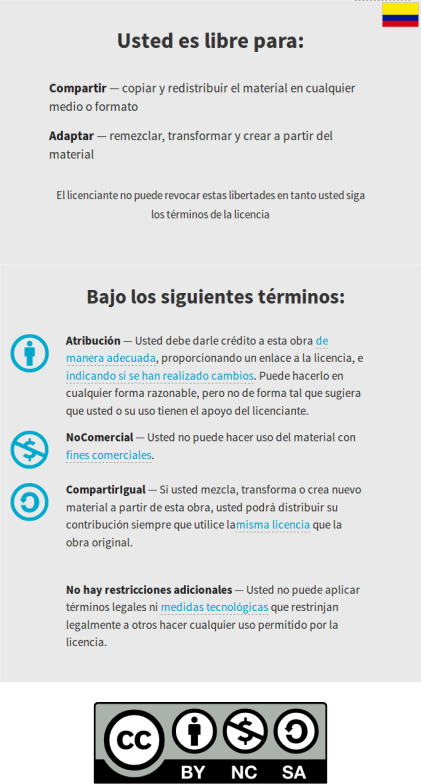
\includegraphics[width=0.65\linewidth]{img/License/licencia}
\end{center}

}

\portada 
\thispagestyle{empty}

\newpage\null\thispagestyle{empty}\newpage

\contraportada
\thispagestyle{empty}
\newpage\null\thispagestyle{empty}\newpage

\thispagestyle{empty}
\newpage

%\begin{abstractpage}\addcontentsline{toc}{chapter}{Abstract}
%	% $Log: abstract.tex,v $
% Revision 1.1  93/05/14  14:56:25  starflt
% Initial revision
%
% Revision 1.1  90/05/04  10:41:01  lwvanels
% Initial revision
%
%
%% The text of your abstract and nothing else (other than comments) goes here.
%% It will be single-spaced and the rest of the text that is supposed to go on
%% the abstract page will be generated by the abstractpage environment.  This
%% file should be \input (not \include 'd) from cover.tex.
La tomografía óptica de coherencia (OCT) es una técnica de imagen médica \textit{no-invasiva} que se basa en interferometría de baja coherencia para producir imágenes con alta resolución axial y lateral de medio inhomogéneos como tejidos. OCT ha visto un alto desarrollo científico y clínico debido a que llena un vacío de resolución existente entre el ultrasonido y la microscopía confocal. La investigación en OCT ha crecido exponencialmente en los últimos años, registrándose alrededor de treinta mil artículos desde su descubrimiento en 1991 hasta el 2015, relacionando las diversas áreas que abarca. Este trabajo está centrado en el entendimiento de los principio básicos y el desarrollo de nuevas técnicas de posprocesamiento para datos provenientes de OCT.

La primera parte del trabajo de grado está orientado a la implementación de los conceptos básicos de OCT para recrear un sistema óptico que permite analizar muestras \textit{ex-vivo}. En el montaje experimental se obtuvo una resolución axial de $\approx2\mu m$ y una resolución lateral de $\approx3 \mu m$, con un escaneo máximo de $\approx1.5mm$ en profundidad y $\approx2.5mm$ de manera lateral, lo que permitió analizar muestras pequeñas. Sin embargo, pese a las regulaciones existentes para el análisis \textit{in-vivo}, el montaje se probó en aplicaciones no médicas de OCT. Las primeras pruebas se realizaron en el escaneo de la topografía de una moneda, en donde se obtuvo una reconstrucción detallada del relieve que esta posee, las mediciones indicaron alturas máximas de $\approx50\mu m$. La segunda muestra que se estudió fue el ala frontal de un insecto \textit{ex-vivo}, donde se pudieron observar estructuras internas tales como la membrana. En este caso, se midió el espesor de la membrana, obteniéndose $\approx5\mu m$.

En la segunda parte del trabajo de grado, se planteó un nuevo método de filtrado de ruido por \speckle a partir del conocimiento de las causas y las características que éste posee, tomando elementos de técnicas de filtrado proveniente de las imágenes de radares de apertura sintética SAR. El algoritmo, conocido como \textit{non-loca means} (\textit{nlmeans}) fue planteado para el caso de ruido blanco, y gracias a sus resultados, ha sido extendido a diversas técnicas de imagen, entre ellas, imágenes SAR, en donde la obtención de los datos hace que también se de la presencia de ruido por \textit{speckle}. Modificando el funcionamiento de \nlmeans en el caso de ruido por \speckle y considerando las características de los datos disponibles en OCT, se propuso una modificación a \nlmeans denotada como \textit{NL-Means-OCT}. En \nlmeansOCT hay una combinación de los conceptos tradicionales de \nlmeans junto con otras implementaciones tridimensionales, lo que convierte a \nlmeansOCT en una herramienta útil para filtrar datos de OCT en donde es necesario la preservación de estructuras finas, o que se encuentran alteradas por la presencia de desplazamientos producidos por el paciente. Los resultados del filtrado con \nlmeansOCT mostraron conservar la fidelidad en la imagen mientras se elimina el ruido por \textit{speckle}. Dadas las características de \nlmeansOCT se pudo implementar de manera satisfactoria en otras áreas en desarrollo de OCT, entre ellas tractografía y gastroenterología.

La última parte del trabajo consistió en el planteamiento de un nuevo método para la corrección de problemas en la fase de un sistema de OCT a partir de fuente de barrido. El problema de la fase surge porque la fuente de barrido tiene fluctuaciones de sincronía con el fotodetector, por lo que la fase del tomograma puede sufrir alteraciones. En vista de que son pocos los algoritmos existentes para abordar este problema, se planteó un método de solución a partir de una optimización, tomando como función objetivo los espectros de potencia asociados con el tomograma, de manera que el espectro de potencia del tomograma afectado se aproxima al de un tomograma ideal mediante una minimización. Aplicando conceptos del enfoque en medios turbios, la implementación muestra encontrar de manera satisfactoria los mapas de corrupción en la fase. Las simulaciones indican que el algoritmo puede encontrar una buena representación del mapa de corrupción real a partir de la aproximación de valores mediante una función de mérito. Los resultados experimentales preliminares verifican la hipótesis de que este modelo mejora los planteamientos actuales de otros autores.


%\end{abstractpage}

\dedicatoria
\newpage\null\thispagestyle{empty}\newpage

\licencia
\addcontentsline{toc}{chapter}{Licencia}
\newpage\null\thispagestyle{empty}\newpage


%\begin{resumen}
%	\addcontentsline{toc}{chapter}{Abstract}
%	% $Log: abstract.tex,v $
% Revision 1.1  93/05/14  14:56:25  starflt
% Initial revision
%
% Revision 1.1  90/05/04  10:41:01  lwvanels
% Initial revision
%
%
%% The text of your abstract and nothing else (other than comments) goes here.
%% It will be single-spaced and the rest of the text that is supposed to go on
%% the abstract page will be generated by the abstractpage environment.  This
%% file should be \input (not \include 'd) from cover.tex.
La tomografía óptica de coherencia (OCT) es una técnica de imagen médica \textit{no-invasiva} que se basa en interferometría de baja coherencia para producir imágenes con alta resolución axial y lateral de medio inhomogéneos como tejidos. OCT ha visto un alto desarrollo científico y clínico debido a que llena un vacío de resolución existente entre el ultrasonido y la microscopía confocal. La investigación en OCT ha crecido exponencialmente en los últimos años, registrándose alrededor de treinta mil artículos desde su descubrimiento en 1991 hasta el 2015, relacionando las diversas áreas que abarca. Este trabajo está centrado en el entendimiento de los principio básicos y el desarrollo de nuevas técnicas de posprocesamiento para datos provenientes de OCT.

La primera parte del trabajo de grado está orientado a la implementación de los conceptos básicos de OCT para recrear un sistema óptico que permite analizar muestras \textit{ex-vivo}. En el montaje experimental se obtuvo una resolución axial de $\approx2\mu m$ y una resolución lateral de $\approx3 \mu m$, con un escaneo máximo de $\approx1.5mm$ en profundidad y $\approx2.5mm$ de manera lateral, lo que permitió analizar muestras pequeñas. Sin embargo, pese a las regulaciones existentes para el análisis \textit{in-vivo}, el montaje se probó en aplicaciones no médicas de OCT. Las primeras pruebas se realizaron en el escaneo de la topografía de una moneda, en donde se obtuvo una reconstrucción detallada del relieve que esta posee, las mediciones indicaron alturas máximas de $\approx50\mu m$. La segunda muestra que se estudió fue el ala frontal de un insecto \textit{ex-vivo}, donde se pudieron observar estructuras internas tales como la membrana. En este caso, se midió el espesor de la membrana, obteniéndose $\approx5\mu m$.

En la segunda parte del trabajo de grado, se planteó un nuevo método de filtrado de ruido por \speckle a partir del conocimiento de las causas y las características que éste posee, tomando elementos de técnicas de filtrado proveniente de las imágenes de radares de apertura sintética SAR. El algoritmo, conocido como \textit{non-loca means} (\textit{nlmeans}) fue planteado para el caso de ruido blanco, y gracias a sus resultados, ha sido extendido a diversas técnicas de imagen, entre ellas, imágenes SAR, en donde la obtención de los datos hace que también se de la presencia de ruido por \textit{speckle}. Modificando el funcionamiento de \nlmeans en el caso de ruido por \speckle y considerando las características de los datos disponibles en OCT, se propuso una modificación a \nlmeans denotada como \textit{NL-Means-OCT}. En \nlmeansOCT hay una combinación de los conceptos tradicionales de \nlmeans junto con otras implementaciones tridimensionales, lo que convierte a \nlmeansOCT en una herramienta útil para filtrar datos de OCT en donde es necesario la preservación de estructuras finas, o que se encuentran alteradas por la presencia de desplazamientos producidos por el paciente. Los resultados del filtrado con \nlmeansOCT mostraron conservar la fidelidad en la imagen mientras se elimina el ruido por \textit{speckle}. Dadas las características de \nlmeansOCT se pudo implementar de manera satisfactoria en otras áreas en desarrollo de OCT, entre ellas tractografía y gastroenterología.

La última parte del trabajo consistió en el planteamiento de un nuevo método para la corrección de problemas en la fase de un sistema de OCT a partir de fuente de barrido. El problema de la fase surge porque la fuente de barrido tiene fluctuaciones de sincronía con el fotodetector, por lo que la fase del tomograma puede sufrir alteraciones. En vista de que son pocos los algoritmos existentes para abordar este problema, se planteó un método de solución a partir de una optimización, tomando como función objetivo los espectros de potencia asociados con el tomograma, de manera que el espectro de potencia del tomograma afectado se aproxima al de un tomograma ideal mediante una minimización. Aplicando conceptos del enfoque en medios turbios, la implementación muestra encontrar de manera satisfactoria los mapas de corrupción en la fase. Las simulaciones indican que el algoritmo puede encontrar una buena representación del mapa de corrupción real a partir de la aproximación de valores mediante una función de mérito. Los resultados experimentales preliminares verifican la hipótesis de que este modelo mejora los planteamientos actuales de otros autores.


%\end{resumen}


\cleardoublepage
\begin{center}
\section*{Agradecimientos}
\end{center}
Quisiera agradecer en primera instancia a mi familia por el apoyo que han dado durante este nuevo capítulo de mi vida. A René y a Néstor por estos años de discusiones, alegatos, frustraciones, asesorías y buenos resultados que hemos obtenido, y que han propiciado un ambiente de trabajo ameno como \textit{compañeros}. A Sebastián por la ayuda con los experimentos. A los compañeros del laboratorio, Camilo con su sentido del humor, Manuela con sus pataletas de niña burgués, y Mateito perrito. A Luciano, por haberme invitado a hacer parte del laboratorio desde hace unos años. Finalmente, a la universidad EAFIT por el apoyo económico mediante los proyectos internos que me permitieron estudiar la Maestría.
\addcontentsline{toc}{chapter}{Agradecimientos}
\newpage\null\thispagestyle{empty}\newpage

\begin{abstract}
	\addcontentsline{toc}{chapter}{Resumen}
	% $Log: abstract.tex,v $
% Revision 1.1  93/05/14  14:56:25  starflt
% Initial revision
%
% Revision 1.1  90/05/04  10:41:01  lwvanels
% Initial revision
%
%
%% The text of your abstract and nothing else (other than comments) goes here.
%% It will be single-spaced and the rest of the text that is supposed to go on
%% the abstract page will be generated by the abstractpage environment.  This
%% file should be \input (not \include 'd) from cover.tex.
La tomografía óptica de coherencia (OCT) es una técnica de imagen médica \textit{no-invasiva} que se basa en interferometría de baja coherencia para producir imágenes con alta resolución axial y lateral de medio inhomogéneos como tejidos. OCT ha visto un alto desarrollo científico y clínico debido a que llena un vacío de resolución existente entre el ultrasonido y la microscopía confocal. La investigación en OCT ha crecido exponencialmente en los últimos años, registrándose alrededor de treinta mil artículos desde su descubrimiento en 1991 hasta el 2015, relacionando las diversas áreas que abarca. Este trabajo está centrado en el entendimiento de los principio básicos y el desarrollo de nuevas técnicas de posprocesamiento para datos provenientes de OCT.

La primera parte del trabajo de grado está orientado a la implementación de los conceptos básicos de OCT para recrear un sistema óptico que permite analizar muestras \textit{ex-vivo}. En el montaje experimental se obtuvo una resolución axial de $\approx2\mu m$ y una resolución lateral de $\approx3 \mu m$, con un escaneo máximo de $\approx1.5mm$ en profundidad y $\approx2.5mm$ de manera lateral, lo que permitió analizar muestras pequeñas. Sin embargo, pese a las regulaciones existentes para el análisis \textit{in-vivo}, el montaje se probó en aplicaciones no médicas de OCT. Las primeras pruebas se realizaron en el escaneo de la topografía de una moneda, en donde se obtuvo una reconstrucción detallada del relieve que esta posee, las mediciones indicaron alturas máximas de $\approx50\mu m$. La segunda muestra que se estudió fue el ala frontal de un insecto \textit{ex-vivo}, donde se pudieron observar estructuras internas tales como la membrana. En este caso, se midió el espesor de la membrana, obteniéndose $\approx5\mu m$.

En la segunda parte del trabajo de grado, se planteó un nuevo método de filtrado de ruido por \speckle a partir del conocimiento de las causas y las características que éste posee, tomando elementos de técnicas de filtrado proveniente de las imágenes de radares de apertura sintética SAR. El algoritmo, conocido como \textit{non-loca means} (\textit{nlmeans}) fue planteado para el caso de ruido blanco, y gracias a sus resultados, ha sido extendido a diversas técnicas de imagen, entre ellas, imágenes SAR, en donde la obtención de los datos hace que también se de la presencia de ruido por \textit{speckle}. Modificando el funcionamiento de \nlmeans en el caso de ruido por \speckle y considerando las características de los datos disponibles en OCT, se propuso una modificación a \nlmeans denotada como \textit{NL-Means-OCT}. En \nlmeansOCT hay una combinación de los conceptos tradicionales de \nlmeans junto con otras implementaciones tridimensionales, lo que convierte a \nlmeansOCT en una herramienta útil para filtrar datos de OCT en donde es necesario la preservación de estructuras finas, o que se encuentran alteradas por la presencia de desplazamientos producidos por el paciente. Los resultados del filtrado con \nlmeansOCT mostraron conservar la fidelidad en la imagen mientras se elimina el ruido por \textit{speckle}. Dadas las características de \nlmeansOCT se pudo implementar de manera satisfactoria en otras áreas en desarrollo de OCT, entre ellas tractografía y gastroenterología.

La última parte del trabajo consistió en el planteamiento de un nuevo método para la corrección de problemas en la fase de un sistema de OCT a partir de fuente de barrido. El problema de la fase surge porque la fuente de barrido tiene fluctuaciones de sincronía con el fotodetector, por lo que la fase del tomograma puede sufrir alteraciones. En vista de que son pocos los algoritmos existentes para abordar este problema, se planteó un método de solución a partir de una optimización, tomando como función objetivo los espectros de potencia asociados con el tomograma, de manera que el espectro de potencia del tomograma afectado se aproxima al de un tomograma ideal mediante una minimización. Aplicando conceptos del enfoque en medios turbios, la implementación muestra encontrar de manera satisfactoria los mapas de corrupción en la fase. Las simulaciones indican que el algoritmo puede encontrar una buena representación del mapa de corrupción real a partir de la aproximación de valores mediante una función de mérito. Los resultados experimentales preliminares verifican la hipótesis de que este modelo mejora los planteamientos actuales de otros autores.


	%\newpage\null\thispagestyle{empty}\newpage
\end{abstract}

\pagestyle{plain}
  % -*- Mode:TeX -*-
%% This file simply contains the commands that actually generate the table of
%% contents and lists of figures and tables.  You can omit any or all of
%% these files by simply taking out the appropriate command.  For more
%% information on these files, see appendix C.3.3 of the LaTeX manual. 
\tableofcontents
\newpage
\listoffigures
%\newpage
%\listoftables

\newpage
\chapter*{Lista de acrónimos}
\addcontentsline{toc}{chapter}{Lista de acrónimos}
\thispagestyle{plain}
\noindent\textbf{CT} - Computed tomography - Tomografía computacional.\\ 
\textbf{CT X-Ray} - Computed X ray tomography - Tomografía computarizada de rayos X.\\
\textbf{DAQ} - Data adquisition - Adquisión de datos.\\ 
\textbf{ENL} - Equivalent number of looks - Número equivalente de vistas.\\
\textbf{FDOCT} - Frequency-domain optical coherence tomography - Tomografía óptica de coherencia en el dominio frecuencial.\\ 
\textbf{FFOCT} - Full-field optical coherence tomography - Tomografía óptica de coherencia de campo completo.\\ 
\textbf{FOM} - Function of merit - Función de mérito.\\
\textbf{FWHM} - Full-width at half maxima - Anchura a la mitad del máximo.\\ 
\textbf{IPS} - Iterative phase shifting - Salto de fase iterativo.\\
\textbf{MEMS} - Microelectromecanic system - Sistema microelectromecánico.\\
\textbf{MRI} - Magnetic resonance imaging - Imagen de resonancia magnética.\\ 
\textbf{MSBTD} - Multiscale sparsity-based tomographic denoising .\\ 
\textbf{NA} - Numerical aperture - Apertura numérica.\\ 
\textbf{NL-Means} - Non-local means.\\ 
\textbf{NL-Means-OCT} - Non-local means in optical coherence tomography - Non-local means en tomografía óptica de coherencia.\\ 
\textbf{NL-Means con PPB} - Non-local means with probabilistic patch-based weights .\\
\textbf{NURD} - Non-uniform rotational distortion - Distorsión rotacional no uniforme.\\
\textbf{OCM} - Optical coherence microscopy - Microscopía óptica de coherencia.\\ 
\textbf{OCT} - Optical coherence tomography - Tomografía óptica de coherencia.\\ 
\newpage
\thispagestyle{plain}
\noindent\textbf{OFDI} - Optical frequency domain imaging - Imagen óptica en el dominio frecuencial.\\ 
\textbf{PPB} - Probabilistic patch-based weigths.\\
\textbf{PS} - Power spectrum - Espectro de potencia.\\ \textbf{PSF} - Point-spread function - Función de dispersión de punto.\\ 
\textbf{SAR} - Synthetic aperture radar - Radar de apertura sintética.\\ 
\textbf{SBOCT} - Spectrometer-based optical coherence tomography - Tomografía óptica de coherencia basada en espectrómetro.\\ 
\textbf{SNR} - Signal-to-noise ratio - Relación señal-ruido.\\ 
\textbf{SPECT} - Single-photon emision computed tomography - Tomografía computarizada de emisión monofotónica.\\ 
\textbf{SSOCT} - Swept-source optical coherence tomography - Tomografía óptica de coherencia con fuente de barrido.\\ 
\textbf{TDOCT} - Time-domain optical coherence tomography - Tomografía óptica de coherencia en el dominio temporal.\\
\textbf{US} - Ultrasound imaging - Imagen de ultrasonido.\\  



%now start the fancy headings
\pagestyle{fancyplain}
\addtolength{\headheight}{\baselineskip}
%add a nice little line underneath the heading
\renewcommand{\headrulewidth}{0.6pt}

%% This is an example first chapter.  You should put chapter/appendix that you
%% write into a separate file, and add a line \include{yourfilename} to
%% main.tex, where `yourfilename.tex' is the name of the chapter/appendix file.
%% You can process specific files by typing their names in at the 
%% \files=
%% prompt when you run the file main.tex through LaTeX.
\chapter{Introducción}
\label{chapter:intro}

Hasta finales del siglo XIX, las herramientas disponibles para el diagnóstico médico y el estudio de patologías en el cuerpo humano se limitaban esencialmente al microscopio, inventado a finales del siglo XVI, el termómetro a mediados del siglo XVII y el estetoscopio a inicios del siglo XIX. A partir de estas herramientas y la observación del crecimiento, desarrollo y evolución de patologías en el cuerpo humano, se determinaron las características de los trastornos producidos por enfermedades en órganos de fácil acceso, tales como la lengua, los ojos y los oídos. Sin embargo, hasta finales del siglo XIX no existía un examen que permitiera obtener información de la condición y funcionamiento de los órganos al interior del cuerpo, aunque sería en 1896 cuando Wilhelm Röntgen descubriera las propiedades de los rayos X para penetrar el interior de tejidos vivos y obtener información del cuerpo desconocida hasta la fecha \cite{Guy2005}. El descubrimiento de los rayos X marcó, además de una revolución en los exámenes médicos, uno de los mayores puntos de unión entre la física, química, ingeniería y en general, las ciencias exactas con la medicina.

%Desde sus inicios, la relación entre ciencia y medicina no ha sido directa. La ciencia, por un lado, está basada en principios teóricos con fundamentos matemáticos o físicos que permiten \emph{predecir} el resultado de un evento bajo ciertas condiciones, como la resistencia de un puente según las leyes de Newton o el campo magnético generado por cargas en movimiento con las leyes de Maxwell. La medicina, por su parte, se basa en la \emph{observación empírica} de los efectos que conlleva la presencia de algún trastorno en el cuerpo humano, por ejemplo, la fiebre o la aparición de sarpullido. Más que una relación directa, se podría encontrar una unión en el desarrollo de la medicina paralelo al de la ciencia. En este sentido, el desarrollo de nuevas teorías como la física nuclear o el ultrasonido, han traído la creación de nuevos procedimientos y dispositivos que facilitan la comprensión del cuerpo humano. Como ilustración de esta relación, la segunda guerra mundial vista desde una perspectiva de avance científico, trajo consigo cuatro grandes desarrollos: la física nuclear, la electrónica digital, la computación y la radio de alta frecuencia; a partir de estos avances, surge la tomografía computacional de rayos X, que en la actualidad es ampliamente utilizado en el diagnóstico.

Desde sus inicios, la relación entre ciencia y medicina no ha sido directa. La ciencia, por un lado, está basada en principios teóricos con fundamentos matemáticos o físicos que permiten \emph{predecir} el resultado de un evento bajo ciertas condiciones, como la resistencia de un puente según las leyes de Newton o el campo magnético generado por cargas en movimiento con las leyes de Maxwell. La medicina, por su parte, se basa en la \emph{observación empírica} de los efectos que conlleva la presencia de algún trastorno en el cuerpo humano, por ejemplo, la fiebre o la aparición de sarpullido. Más que una relación directa, se podría encontrar la unión entre medicina y ciencia en el desarrollo paralelo de ambas áreas. En este sentido, la aparición de nuevas teorías como la física nuclear, han traído consigo la creación de nuevos procedimientos y dispositivos que facilitan la comprensión del cuerpo humano. Como ilustración de esta relación, se encuentra la segunda guerra mundial, que vista desde una perspectiva de avance científico, trajo consigo cuatro grandes desarrollos: la física nuclear, la electrónica digital, la computación y la radio de alta frecuencia \cite{Dhawan2008}; a partir de estos avances, surge la tomografía computacional de rayos X y el ultrasonido, que en la actualidad son ampliamente utilizados en el diagnóstico médico.

En este punto de unión entre ciencia y medicina, una de las áreas que más fuertemente las relaciona son las técnicas de \emph{imagen médica}, cuyo objetivo es brindar imágenes de información relevante de estructuras y/o funciones internas del cuerpo mediante instrumentación y teorías especializadas \cite{Guy2005}. En el entorno clínico, las imágenes de órganos, partes o funciones específicas del cuerpo permiten realizar exámenes diagnósticos de una enfermedad o patología, esto es de alta importancia si se considera que es posible estudiar la progresión, avance o crecimiento de una enfermedad asociándolo con el cambio físico que produce \cite{Beutel2009}. En el entorno científico, producir imágenes médicas es una tarea altamente multidisciplinar, ya que requiere no solo el desarrollo teórico y de investigación, sino que acarrea consigo la creación de dispositivos y plataformas que sean de alta compatibilidad, fácil acceso, bajo costo y de implementación sencilla. Algunas de las técnicas de imagen médica más relevantes actualmente son: la tomografía computarizada de rayos X (CT X-ray) \cite{Cierniak2011}, la imagen de resonancia magnética (MRI) \cite{Haacke1999}, la imagen de ultrasonido (\textit{ultrasound imaging}) \cite{Szabo}, la tomografía computarizada de emisión monofotónica (SPECT) \cite{Sharp2005} y la tomografía óptica de coherencia (OCT) \cite{Drexler2015}.

%En alineación con el desarrollo ciencia/medicina, la tomografía óptica de coherencia, ampliamente conocida por sus siglas en inglés como OCT (\textit{optical coherence tomography}), es una técnica de imagen médica surgida en 1991, cuyo propósito es obtener imágenes con alta resolución de la sección transversal o imágenes volumétricas de microestructuras internas en tejidos biológicos. 

La tomografía óptica de coherencia, ampliamente conocida por sus siglas en inglés como OCT (\textit{optical coherence tomography}), es una técnica de imagen médica cuyo propósito es obtener imágenes con alta resolución de la sección transversal o imágenes volumétricas de microestructuras internas en tejidos biológicos. A continuación, se mostrará el desarrollo e importancia que reviste OCT para el diagnóstico médico actual.

\iffalse

Historia:
 -> Guerras mundiales -> Desarrollo ciencia -> Conocimiento apenas en uso -> Medicina -> Tipos de análisis con ciencia (microscopía, radiografía con rayos X, tomografía computacional de rayos X, imagen de resonancia magnética, ultrasonido, OCT)
\fi

\section{Tomografía óptica de coherencia y su papel en medicina}

\subsection{Tomografía óptica de coherencia (OCT)}

En los últimos años han aparecido nuevas técnicas para la toma de imágenes en múltiples disciplinas científicas, entre ellas destacan por su alta actividad de investigación, la formación de imágenes biomédicas, impulsada principalmente por el constante desarrollo de dispositivos para telecomunicaciones que han permitido la producción de instrumentos electromagnéticos de alto desempeño a costos relativamente bajos. Como consecuencia de esto, múltiples técnicas para el escaneo de materiales con un índice de esparcimiento alto, como los tejidos biológicos han sido creadas. De estas técnicas surge la tomografía, que es particularmente interesantes por su potencial para realizar imágenes que ayudan al diagnóstico médico a través de exámenes \emph{no-invasivos}. La tomografía en general, se basa en la creación de ``cortes''  de objetos tridimensionales, que en conjunto generan una imagen en dos o tres dimensiones de la muestra en cuestión. \emph{OCT es una técnica no-invasiva de imagen tridimensional capaz de producir imágenes con alta resolución lateral y axial a través de muestras esparsivas e inhomogéneas, tales como los tejidos biológicos} \cite{Tomlins}. En sus inicios, las técnicas de OCT se basaron en medidas de profundidad de baja coherencia en el dominio temporal con un interferómetro de luz blanca. La posibilidad de emplear interferómetros de luz blanca para la formación de imágenes tridimensionales en tejidos biológicos fue liderada por Huang \etal \cite{Huang1991}, quienes propusieron emplear reflectometría de baja coherencia en sistemas biológicos. Su sistema de OCT se basó en múltiples escaneos de una serie de ubicaciones laterales y axiales para proveer un mapa de sitios o lugares en donde la muestra refleja luz. Una de las características más importantes de esta nueva técnica, es que a diferencia de la microscopía confocal, en donde la resolución longitudinal depende de la apertura numérica, en OCT la resolución solo está limitada por la longitud de coherencia de la fuente de luz, por consiguiente, OCT puede tener alta resolución en profundidad aun cuando la apertura del sistema es pequeña.

OCT es una técnica que permite producir imágenes con alta resolución de la sección transversal o volumétricas mediante la medición del ``eco'' producido por la retroreflexión de luz en el tejido \cite{Huang1991}. El ``eco'' se produce cuando un haz de luz llega hasta el tejido y luego es esparcido, de forma que la información recolectada por OCT es únicamente aquella porción de luz retrodispersada o retroreflejada hacia el sistema óptico. Esta característica permite que OCT pueda presentar imágenes \emph{in-situ} y en tiempo real de patologías presentes en los tejidos, lo que la ha convertido en una herramienta útil en el diagnóstico médico, debido a que realiza ``biopsias ópticas'' sin la necesidad de remover o procesar parte del tejido \cite{Brezinski1996}. OCT puede producir imágenes tridimensionales \emph{no-invasivas} de estructuras internas, tales como la mácula \cite{Hee1995_4}, el tracto gastrointestinal \cite{Tearney1997}, las arterias coronarias \cite{Tearney1996_2}, entre otros.

\subsection{OCT en imagen médica}

OCT tiene diversos aspectos que son comunes al ultrasonido y a la microscopía. Por un lado, la resolución axial en imágenes de ultrasonido de alta resolución, se encuentra en el rango típico de $0.1$ hasta $1mm$ y dependerá de la frecuencia de la onda de sonido que se emplee, los valores típicos para la frecuencia varían entre los $3$ y $40MHz$ \cite{Szabo}. No obstante, en este rango de frecuencias es difícil emplear las ondas de sonido en tejidos, ya que éstos además de esparcirlas fuertemente, atenúan completamente las ondas en unos pocos milímetros. Por otro lado, algunas ramas de la microscopía poseen una alta resolución en imagen de tejidos, por ejemplo, la microscopía confocal, cuya resolución es de alrededor de $1\mu m$ o inclusive menor. En la microscopía confocal, la resolución está limitada por la difracción, relacionada a su vez con la apertura numérica del sistema; y su capacidad de producir imagen se encuentra influenciada principalmente por la degradación de la luz en dispersiones no deseadas, lo que produce un bajo contraste en la señal a medir \cite{Pawley}. 

OCT por su lado, llena un vacío de resolución entre el ultrasonido y la microscopía, ya que el rango en el cual se mueve OCT varía entre $1$ y $15 \mu m$, aproximadamente $100$ veces más fino que el ultrasonido, en la Fig.~\ref{fig:OCT_Ultrasound_microscopy} se presenta una comparación de la resolución y profundidad de penetración de diferentes técnicas de imagen médica. La principal limitación en OCT se encuentra en que la luz es altamente esparcida por muchos tejidos, lo que limita la profundidad de penetración a $\sim 2mm$ en muchos casos.
%Mientras que una de sus principales ventajas está en su fácil integración en instrumentos médicos, tales como catéteres, endoscopios, laparoscopios o incluso, agujas quirúrgicas que permite hacer imagen de órganos, o incluso, tejidos sólidos en el cuerpo.
OCT es análogo al ultrasonido con la diferencia de emplear luz en lugar de sonido, su principio básico se centra en medir la magnitud y el tiempo de retraso (``eco'') que producen las ondas al llegar a la muestra, de forma que las retroreflecciones en diferentes distancias permite determinar el tamaño y reconstruir microestructuras \cite{Szabo}. Como la velocidad del sonido es de alrededor de $1300m/s$, el ultrasonido ha impulsado la creación de sensores y métodos de sensado que permitan una alta tasa de recepción de información, lo que a su vez ha incentivado el desarrollo de equipos para OCT, en especial si se considera que la luz viaja a aproximadamente $3\times 10^8 m/s$ y que las tasas de recepción de datos deben ser mucho mayores. Una de las principales ventajas de la analogía OCT/ultrasonido se encuentra en su fácil integración en instrumentos médicos, tales como catéteres, endoscopios, laparoscopios o incluso, agujas quirúrgicas que permite hacer imagen de órganos o tejidos sólidos \invivo en el cuerpo humano~\cite{Tearney1996, Tearney1997_2}.

\begin{figure}[ht!]
	\centering
	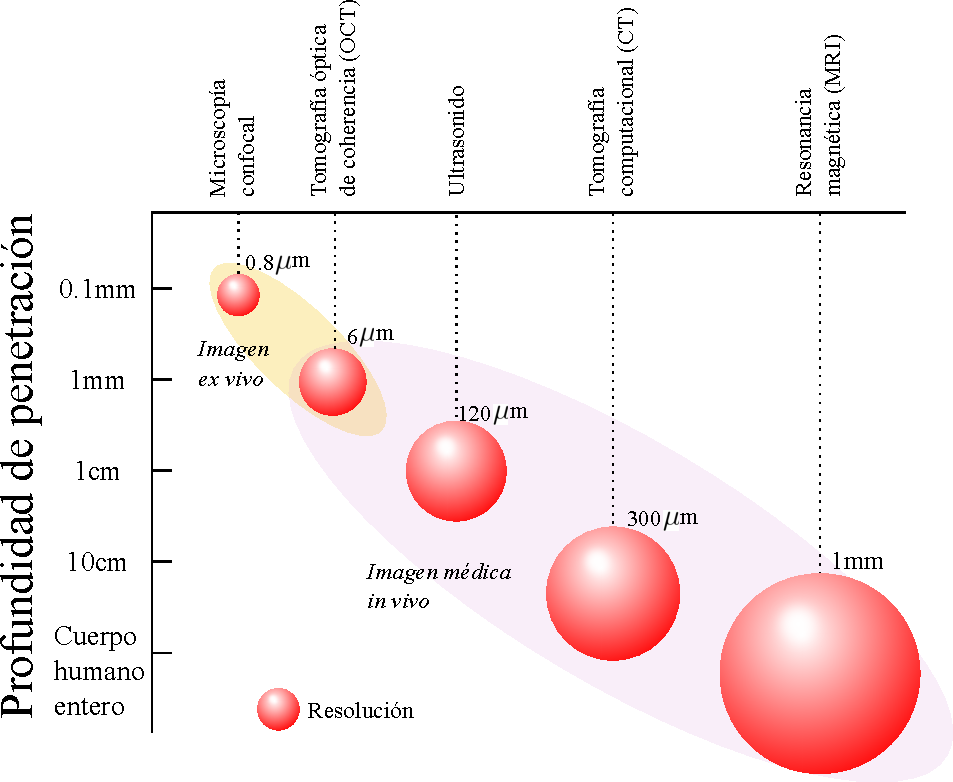
\includegraphics[width = 0.6\textwidth, keepaspectratio]{img/chap1/Carlos_oct_resolucion}
	\caption[Comparación de la resolución de distintas técnicas de imagen médica.]{Comparación de la resolución contra la profundidad de penetración de diferentes modalidades de imagen médica.}
	\label{fig:OCT_Ultrasound_microscopy}
\end{figure}

%La OCT es análoga al ultrasonido, con la diferencia de emplear luz en lugar de sonido. El principio básico de la OCT, es medir la magnitud y el retraso de las retrodipersiones o retroreflecciones de la luz en microestructuras en tejidos, de forma que el tamaño de las microsestructuras puede determinarse a través de la medida del tiempo que tarda el ``eco'' del sonido o la luz en viajar diferentes distancias. El desarrollo de equipos para tratamientos con ultrasonido a su vez ha posibilitado la creación de equipos de bajo costo para OCT, en especial si se considera que la velocidad del sonido es de alrededor de $1300m/s$, mientras que la luz viaja a $3\times 10^8 m/s$. Una de las principales ventajas de la analogía OCT/ultrasonido se encuentra en su fácil integración en instrumentos médicos, tales como catéteres, endoscopios, laparoscopios o incluso, agujas quirúrgicas que permite hacer imagen de órganos o tejidos sólidos \invivo en el cuerpo.



\section{Aplicaciones de OCT}

%\subsection{Los inicios de OCT}

%La propuesta de la técnica de OCT surgió hacia el año 1991 por Huang \etal \cite{Huang1991}, sus primeras pruebas fueron realizadas \emph{ex vivo} en la retina y la arteria coronaria. Huang \etal proponen una técnica análoga al ultrasonido, pero que en lugar de emplear ondas de sonido, emplea luz para realizar reconstrucciones tridimensionales a partir de escaneos bidimensionales, a esta técnica la denominarían tomografía óptica de coherencia, y se basa esencialmente en el empleo de un interferómetro de luz blanca. Con los resultados obtenidos por Huang \etal la OCT se ha posicionado como una de las más grandes aplicaciones emergentes para el diagnóstico oftalmológico e intravascular.

La propuesta de OCT surgió hacia el año 1991 por Huang \etal \cite{Huang1991}, sus primeras pruebas fueron realizadas \exvivo en la retina y la arteria coronaria, y desde estos resultados pudo verse la utilidad de OCT para el diagnóstico oftalmológico e intravascular, áreas en las que ha tenido grandes avances. El ojo humano puede ser analizado ópticamente, es decir, es posible implementar técnicas para observar de manera directa la zona interior del ojo, lo que ha impulsado el uso de métodos de imagen en oftalmología; muchos de los primeros estudios realizados con OCT fueron basados en el ojo humano. Las primeras imágenes \invivo de la retina fueron obtenidas de manera independiente por Fercher \etal \cite{Fercher1993} y Swanson \etal \cite{Swanson1993} en 1993. Estos resultados conllevaron a que en la década de los 90 se diera un alto uso de OCT para el monitoreo, seguimiento, detección y diagnosis de diferentes enfermedades, entre las cuales destaca: enfermedades maculares \cite{Puliafito1995}, incluyendo agujeros maculares \cite{Hee1995_2} y edemas maculares \cite{Hee1995},  coriorretinopatía serosa central \cite{Hee1995_3}, y degeneraciones maculares asociadas a la edad y a la neovascularización coroidal \cite{Hee1995_4}. Un ejemplo de monitoreo con OCT, está en el espesor de las capas de fibra del nervio retinal, el cual es un indicador de glaucoma, y que puede cuantificarse en ojos normales y con glaucoma. Mediante una correlación con medidas convencionales de la estructura y función del nervio óptico es posible encontrar focos de glaucoma, trabajo realizado también a partir de OCT en 1995 por Schuman \etal \cite{Schuman1995}.

La sensibilidad de OCT, en el orden de $-125dB$ o $10^{-12.5}$ veces la luz incidente, permite producir imagen de estructuras tales como la retina que poseen un bajo índice de esparcimiento, sin embargo, la mayor parte de las aplicaciones que emplean OCT requieren la captura de imágenes en tejidos que no son transparentes, y además, producen un alto esparcimiento y dispersión de la luz. En estos casos, es cuando la sensibilidad del método se vuelve relevante, ya que al ser la señal fuertemente atenuada por el esparcimiento, la sensibilidad es quien determina la profundidad hasta la cual se puede conseguir imágenes \cite{Drexler2015}. Las primeras imágenes de tejidos diferentes al ojo fueron posibles mediante el estudio de la influencia de la longitud de onda en el esparcimiento de la luz, en donde se obtuvo que longitudes de onda más largas que el visible reducen el esparcimiento producido por las muestras biológicas e incrementa la profundidad de penetración y la capacidad de producir imagen \cite{Brezinski1996, Schuman1995}. Uno de los primeros estudios del efecto de la longitud de onda sobre las reconstrucciones con OCT fue realizado por Brezinski \etal \cite{Brezinski1996}, quienes hicieron una comparación de imágenes capturadas a $850$ y $1300nm$ \exvivo en una epiglotis humana. La imagen tomada a $1300nm$ mostró una mayor penetración puesto que los principales absorbentes en la mayor parte de los tejidos son la melanina y la hemoglobina, los cuales poseen una alta absorción en el visible y el infrarrojo cercano \cite{Parsa1989}, mientras que la absorción del agua se convierte en dominante para mayores longitudes de onda, alrededor de los $1800-2000nm$. Por otro lado, en la mayoría de los tejidos, el esparcimiento en las longitudes de onda del infrarrojo cercano es uno o dos órdenes de magnitud mayores que la absorción, y éste disminuye para longitudes de onda más grandes.

%\begin{figure}[ht!]
%\centering
%\includegraphics[width = \textwidth, keepaspectratio]{img/oct_longitudes_multiples.png}
%\caption[OCT empleando diferentes longitudes de onda.]{Profundidad de penetración de la OCT en diferentes longitudes de onda. Comparación de la atenuación producida por diferentes longitudes de onda en OCT, visualmente se aprecian más detalles cuando se emplea una longitud de onda de $1300nm$ que con $850nm$. Tomado de \cite{Brezinski1996}.}
%\label{fig:oct_longitudes_multiples}
%\end{figure}

Muchos estudios iniciales de OCT se realizaron \exvivo en especímenes quirúrgicos, estos estudios fueron útiles para definir las estructuras que serían posibles de observar usando OCT \cite{Brezinski1996} y compararlo con la histología. El estudio de la correlación entre las imágenes \exvivo de OCT y la histología se extendió a hasta enfermedades gastrointestinales \cite{Izatt1996, Tearney1997, Kobayashi1998, Pitris2000}, biliares \cite{Tearney1998}, en el aparato reproductor femenino \cite{Pitris1999}, pulmonares \cite{Pitris1998} y urinarias \cite{Tearney1997}.



Los inicios de OCT fueron en oftalmología y hoy en día es una de las áreas con mayor impacto de esta técnica. OCT ha mostrado ser una herramienta bastante útil porque puede identificar característica de enfermedades desde etapas tempranas, permitiendo que se puedan realizar los tratamientos respectivos para prevenir el desarrollo de dichas enfermedades. Además, si se realizan tratamientos periódicos, puede mantenerse un monitoreo de la evolución de la terapia o de la enfermedad. OCT se ha convertido en una técnica importante para el diagnóstico y monitoreo de enfermedades tales como el glaucoma, la degeneración macular relacionada con la edad y la retinopatía diabética, ya que provee información cuantitativa de la patología lo que permite medir el progreso de la enfermedad o la respuesta ante terapias \cite{Hee1998, Schuman1995,Schuman1996}. Las imágenes de OCT proveen medidas cuantitativas de características tales como el espesor o el flujo sanguíneo, estas mediciones han derivado en otras aplicaciones relacionadas con OCT, tales como la obtención de mapas de espesor \cite{Hee1998}, lo que ha permitido generar estándares para la evaluación de algunas patologías presentes mediante la comparación con un estándar.

Otro ejemplo de implementación de OCT es la imagen intravascular. OCT ha permitido obtener imágenes que muestran de forma clara la diferencia entre la túnica íntima, la túnica media y la túnica adventicia al interior de las arterias \cite{Tearney1996_2}. En sus inicios, OCT intravascular \invivo representó un gran desafío, pues debían diseñarse catéteres apropiados para el uso en humanos, además de esto, dado que la sangre esparce altamente la luz, fue necesario la creación de un sistema de flujo para remover la sangre o para diluir los glóbulos rojos en el plano imagen. Los primeros estudios con OCT mediante endoscopios se realizaron en conejos por Fujimoto \etal en 1999 \cite{Fujimoto1999}, por otro lado, hacia el año 2001, Jang \emph{et al.} reportaron la primer imagen mediante OCT en pacientes humanos \cite{Jang2001}. El área intravascular representa una de las áreas actuales más activas en OCT, tanto desde un punto de vista comercial, como desde un punto de vista de investigación.

OCT también ha sido empleada en el caso de la endoscopia. El primer estudio de endoscopia \invivo con imágenes de OCT fue realizado en 1997 \cite{Tearney1997, Sergeev1997}, en donde se obtuvieron los primeros resultados para el análisis del esófago de un conejo. Las imágenes de OCT permitieron diferenciar de manera clara estructuras tales como la mucosa y la serosa. Los primeros estudios de endoscopia con imagen OCT en humanos fueron reportados por Sergeev \etal en 1997 \cite{Sergeev1997} y Feldchtein \etal en 1998 \cite{Feldchtein1998}, quienes mediante una sonda obtuvieron imágenes de membranas mucosas del esófago, la laringe, el estómago, la vejiga urinaria y el cuello uterino; mostrando así la utilidad de OCT en este tipo de imagen clínica.

Dado el crecimiento de casos de cáncer en el esófago, estomago y colon, la endoscopia gastrointestinal tuvo una mayor atención, en contraste con esto, los estudios iniciales de OCT mostraron las ventajas de esta técnica para visualizar estructuras superficiales, ya que permite ver no solo las capas exteriores, sino que adicionalmente puede observar morfologías de tejidos bajo la superficie, permitiendo diferenciar patologías gastrointestinales tales como el esófago de Barret, los pólipos adenomatosos y el adenocarcinoma \cite{Bouma1999, Sergeev1997, Rollins1999, Jackle2000, Jackle2000_2, Sivak2000}. Los estudios de OCT para detección de cáncer son complejos, ya que los resultados de OCT deben ser comparados con técnicas estandarizadas tales como la biopsia, el estándar en la detección de cáncer. El problema que tiene OCT es que el contraste producido por las variaciones en las propiedades esparsivas de diferentes tejidos puede producir errores en las muestras tomadas dada la sensibilidad de OCT.

Gracias a su alta sensibilidad y capacidad para producir imágenes volumétricas \emph{no-invasivas}, OCT ha sido de alto interés en diferentes áreas de la medicina, tales como la oftalmología \cite{Schuman1995, Swanson1993, Puliafito1995, Hee1995, Hee1995_2}, la imagen intravascular mediante catéteres \cite{Grube2002, Jang2002, Bouma2003}, la endoscopia \cite{Tearney1997,Feldchtein1998,Rollins1999}, la detección de cáncer \cite{Sergeev1997,Jackle2000}, la neurociencia \cite{Chen2009,Srinivasan2009,Lee2011}, la cardiología \cite{Li2012,Gu2012,Yazdanfar1997}, la dermatología \cite{Welzel1998,Gambichler2007,Blatter2012}, la odontología \cite{Otis2004,Melo2005,Bakhsh2011}, entre otras áreas.

\section{La investigación en OCT y la participación de América Latina}

Desde sus inicios, OCT ha visto un crecimiento exponencial en la cantidad de publicaciones por año sobre las diversas áreas de la medicina que abarca, así como los dispositivos y procedimientos con los que se realizan las imágenes. Como muestra de este crecimiento, solo en el año 2015 se estima que hubo 3500 publicaciones relacionadas con OCT \cite{Fujimoto2016}, como se muestra en la Fig.~\ref{fig:octpubbyyear}\footnote{Datos tomados de PUBMED.}. El área donde se realiza la mayor cantidad de publicaciones corresponde a oftalmología, seguida por el área cardiovascular y en tercer lugar, el desarrollo tecnológico, sin embargo, también desatacan otras áreas como la dermatología, odontología, neurología, entre otras. El gran desarrollo que ha tenido OCT está fuertemente relacionado con la aceptación a nivel clínico que ha tenido esta técnica, convirtiéndose en estándar para algunos procedimientos diagnósticos. En oftalmología, se estima que 30 millones de exámenes relacionados con OCT son realizados por año alrededor del mundo, y que aproximadamente 100 mil evaluaciones cardiovasculares por año son realizadas con OCT. 

\begin{figure}[ht!]
	\centering
	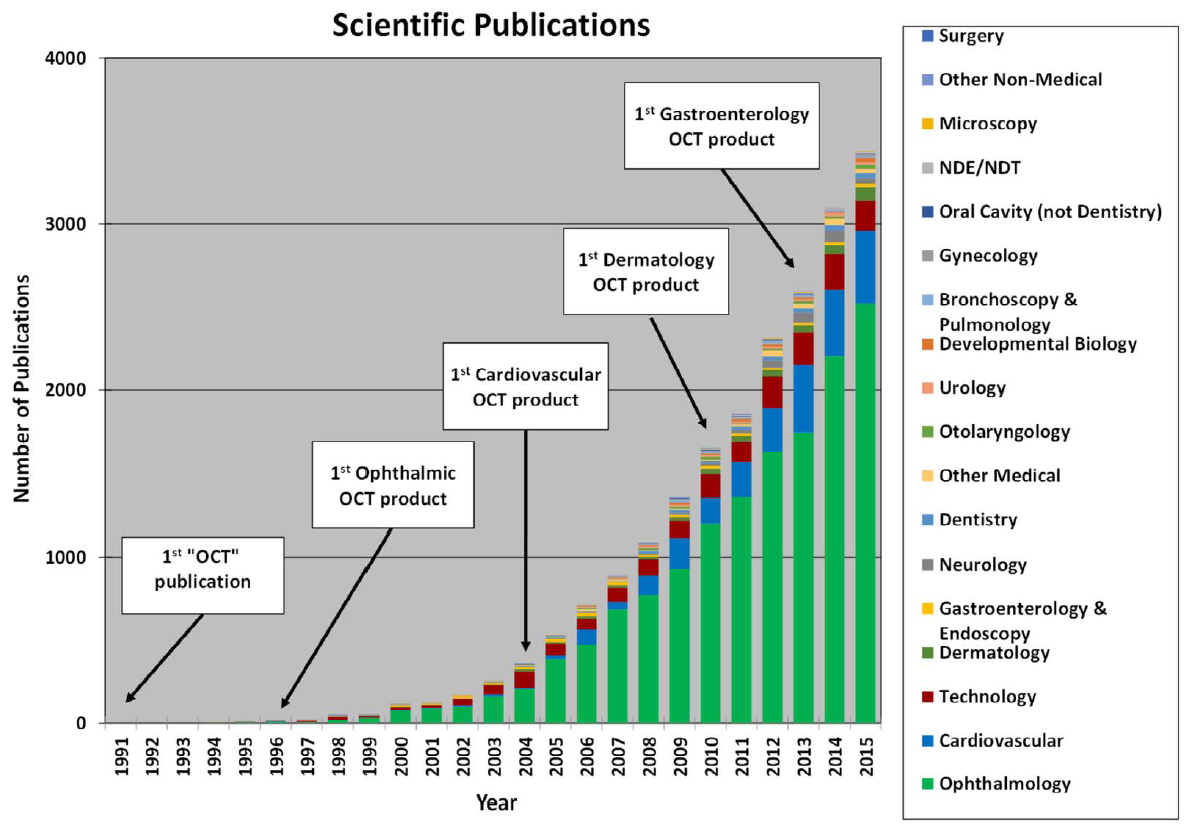
\includegraphics[width=0.7\linewidth]{img/chap1/oct_pub_by_year.png}
	\caption[Publicaciones de OCT por año.]{Publicaciones relacionadas con el desarrollo y aplicaciones de OCT por año. Oftalmología es la categoría más investigada, seguida por el área cardiovascular, y los dispositivos y técnicas en tercer lugar.}
	\label{fig:octpubbyyear}
\end{figure}

El crecimiento exponencial de la cantidad de publicaciones relacionadas con OCT, también se debe a la creación de empresas que comercializan equipos especializados tanto para el diagnóstico como para investigación. OCT ha crecido como un mercado atractivo para diversas compañías de equipos ópticos a nivel mundial, como lo son Zeiss o Thorlabs. En este sentido, el mercado que mueve OCT se estima en unos 700 millones de dólares anuales, como se muestra en la Fig.~\ref{subfig:octmarket}. Por otro lado, el 75\% de las compañías que producen equipos para OCT han surgido como \textit{start-ups} de las universidades que lideran el desarrollo científico de OCT, entre ellas, MIT y Harvard. En la Fig.~\ref{subfig:octcompaniesa} se muestra el crecimiento de las compañías que comercializan productos para diagnóstico e investigación con OCT.

\begin{figure}[ht!]
	\centering
	\subfigure[Mercado estimado de la comercialización de equipos de OCT.]{\label{subfig:octmarket}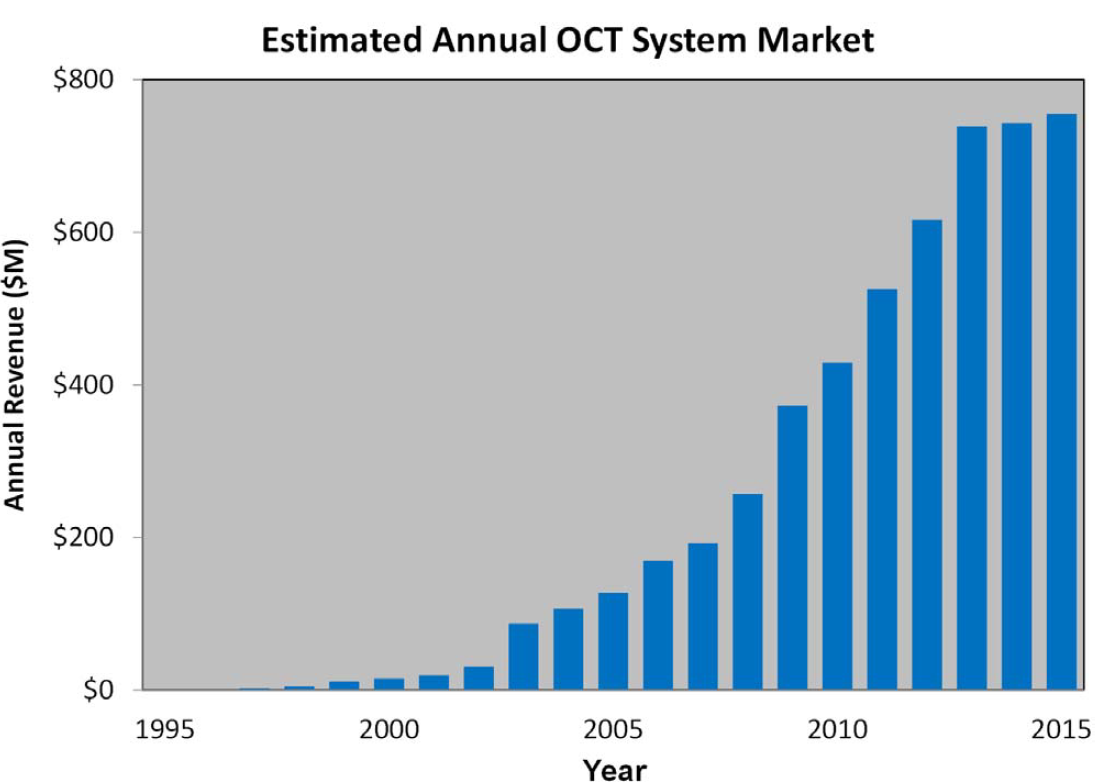
\includegraphics[width=0.45\linewidth]{img/chap1/oct_market}}
	\subfigure[Compañías relacionadas con equipos de OCT.]{\label{subfig:octcompaniesa}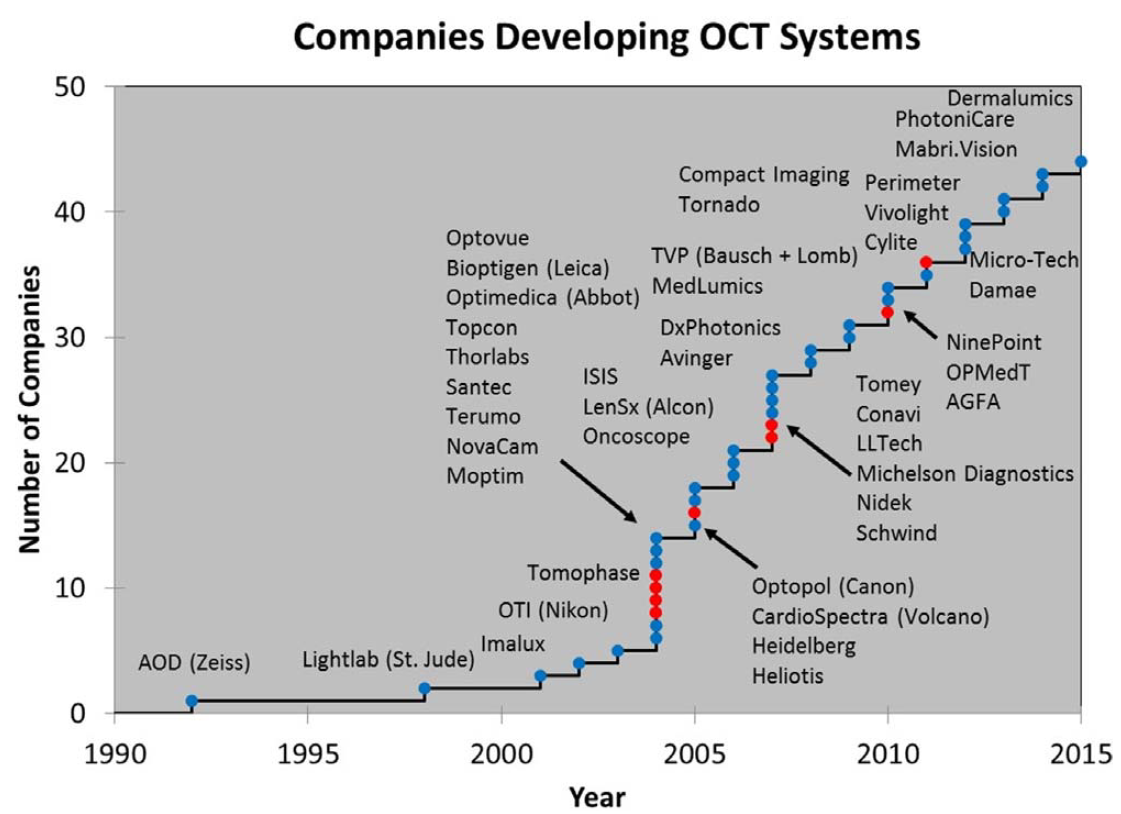
\includegraphics[width=0.45\linewidth]{img/chap1/oct_companiesa}}
	\caption[Mercado relacionado con OCT en los últimos años]{Mercado relacionado con OCT en los últimos años, hacia 2015 se estiman ingresos por $\approx700$ millones de dólares. La cantidad de compañías envueltas en OCT ha crecido a más de 45 en los últimos años, la mayor parte de estas han surgido como \textit{start-ups} provenientes de universidades (circulos azules).}
	\label{fig:octmarket}
\end{figure}

Aunque OCT ha tenido un crecimiento significativo en el ámbito médico e investigativo, cuando se analiza la participación de América Latina en este crecimiento, el panorama no es alentador. En la Fig.~\ref{fig:octgroups2015} se muestra un mapa de la colaboración entre grupos de investigación relacionados por el desarrollo científico en OCT en el año 2015. Los círculos negros representan la cantidad de grupos de investigación relacionados con el tema, mientras que las líneas grises que los une corresponde a la colaboración que hay entre grupos de investigación. En este mapa, se evidencia que a nivel de Latinoamérica, solamente Brasil cuenta con grupos de investigación trabajando en OCT, siendo la universidad de Coimbra (University of Coimbra), la más representativa. Aun con la gran comunidad internacional aportando a la investigación en OCT, no existe en la mayor parte de Latinoamérica, grupos de investigación que posean líneas de investigación relacionadas con OCT, esto a su vez está relacionado con la carencia de equipos especializados para el diagnóstico de enfermedades en donde OCT es el estándar. 

\begin{figure}[ht!]
	\centering
	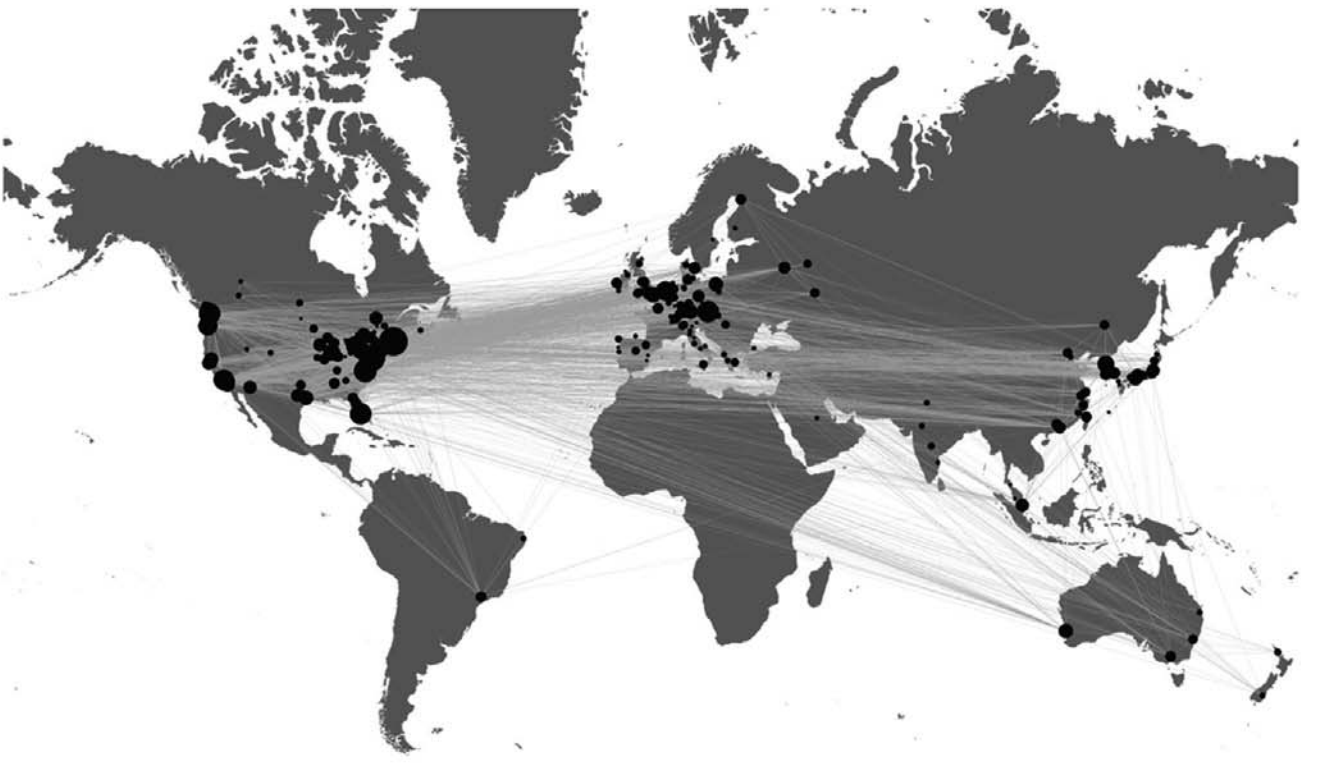
\includegraphics[width=0.7\linewidth]{img/chap1/oct_groups_2015}
	\caption[Mapa de grupos de investigación involucrados en OCT.]{Mapa de grupos de investigación con áreas afines a OCT con sus respectivas colaboraciones. En latinoamérica solo se cuenta con participación de Brasil.}
	\label{fig:octgroups2015}
\end{figure}




%\begin{figure*}
%	\centering
%	
%	\begin{subfigure}[b]{0.3\textwidth}
%		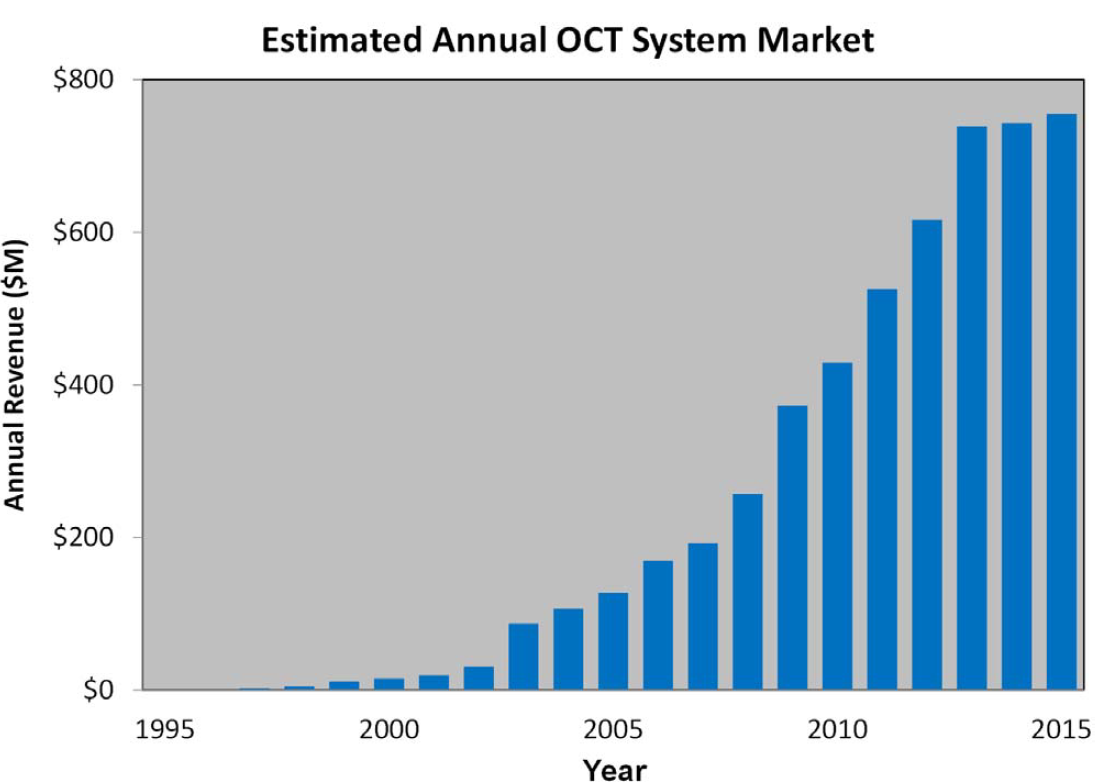
\includegraphics[width=0.4\linewidth]{img/chap1/oct_market}
%	\end{subfigure}%
%	~
%	\begin{subfigure}[b]{0.3\textwidth}
%		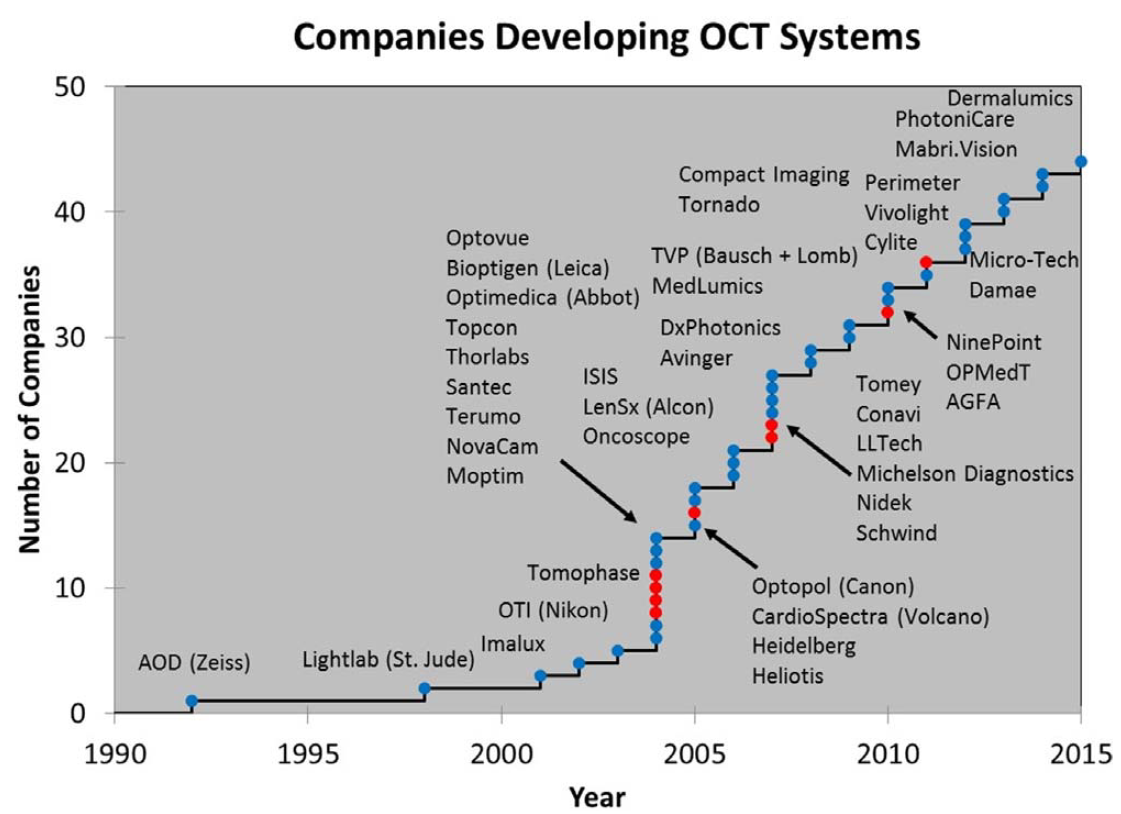
\includegraphics[width=0.4\linewidth]{img/chap1/oct_companiesa}
%	\end{subfigure}
%\end{figure*}


\section{Planteamiento del problema}
\label{sec:plant_problemo}
En la implementación inicial de OCT, la información en profundidad es obtenida mediante desplazamientos axiales del haz de referencia que son producidos por actuadores tales como piezoeléctricos, así como lo indica la Fig.~\ref{fig:scaningsystemoct}. En ese sistema de OCT, la luz producida por la fuente viaja mediante una fibra óptica hasta llegar a un acoplador, en donde se divide por dos caminos diferentes; uno de ellos viaja directamente hasta el espejo de referencia que tiene la posibilidad de desplazarse en sentido axial. Posteriormente, el haz reflejado por el espejo regresa hacia la fibra óptica. El segundo haz es dirigido hacia un espejo de escaneo cuya función es desviar la luz que es proyectada en la muestra de manera controlada. Mediante este sistema, la porción de luz que sea reflejada por la muestra hacia la fibra óptica volverá a incorporarse al sistema óptico regresando hasta el acoplador. La información de los dos haces juntos llega entonces hasta un sensor que se encarga de obtener la señal interferométrica. El sensor transfiere los datos a un sistema de adquisición de datos (DAQ) y finalmente las señales son enviadas hasta el computador. 

La información volumétrica requiere que el haz proyectado hacia la muestra sea desplazado de manera lateral en dos direcciones, procedimiento que se ha realizado a través del uso de sistemas microelectromecánicos (MEMS) que permiten la inclinación controlada del haz, y por tanto el desplazamiento de éste sobre la muestra \cite{Zara2003,Jung2006,Aguirre2007}. El espejo de escaneo se encarga de mover el haz sobre el plano imagen produciendo imágenes bidimensionales de planos $xy$ a profundidades $z$ específicas, a este tipo de imagen se le conoce como \emph{en-face}. Una de las limitaciones de los sistemas para OCT surge justamente en la implementación del sistema de escaneo, ya que hay errores producidos no solo por la instrumentación sino por la misma muestra. 

\begin{figure}[th!]
	\centering
	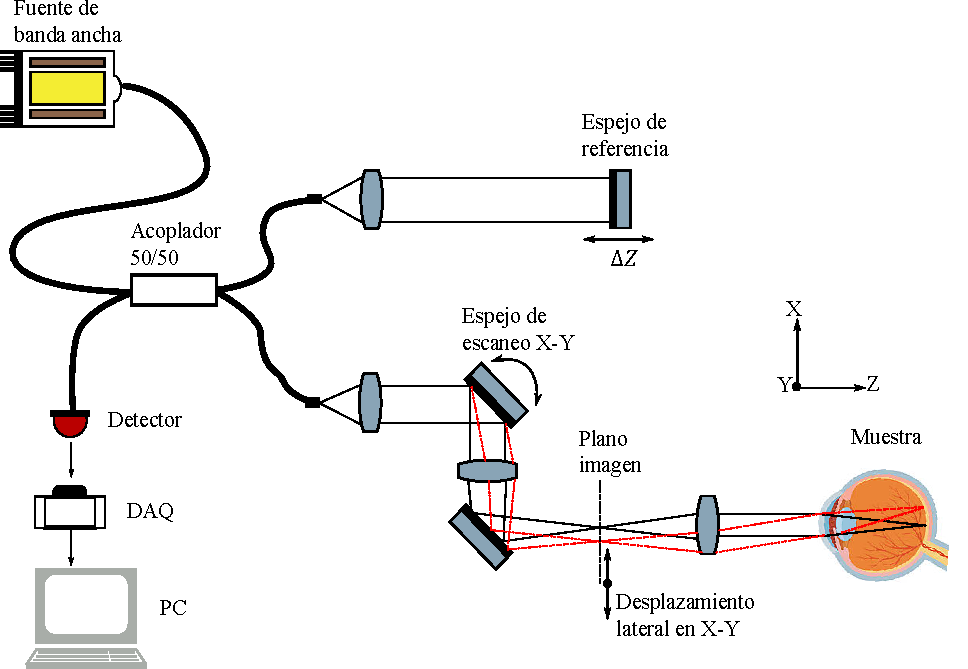
\includegraphics[width=0.7\linewidth]{img/chap1/scaning_system_oc.pdf}
	\caption[Esquema de un sistema de OCT]{Esquema de un sistema de escaneo de OCT para la retina.}
	\label{fig:scaningsystemoct}
\end{figure}


Desde el punto de vista instrumental, algunos espejos de escaneo emplean sistemas de control retroalimentados tales como PID que se encargan del desplazamiento y control del sistema \cite{xie2004}, sin embargo, este tipo de control en lazo cerrado puede tener la falencia de enviar voltajes fluctuantes  que producen desviaciones, y pueden ser causados o bien por las constantes del controlador o por desplazamientos repentinos producidos por el paciente. Otros sistemas basados en MEMS \cite{Strathman2014} requieren voltajes AC para producir respuestas lineales, sin embargo, fluctuaciones en la frecuencia o en la amplitud del voltaje suministrado al actuador producen respuestas diferentes a la esperada. Adicionalmente, mientras se realizan los escaneos axiales, el espejo de escaneo se mueve a velocidad constante en las dos direcciones, por lo tanto hay una dirección con una velocidad menor (\emph{slow-axis}) y otro con una mayor velocidad (\emph{fast-axis}), esto hace necesario una corrección del movimiento en las imágenes de OCT obtenidas \cite{Yun2004, Pierce2005, Drexler2015}. En cuanto a la muestra que es tomada en pacientes, existen diferentes movimientos involuntarios que no pueden ser controlados, tales como la contracción muscular causada por la respiración o el parpadeo, así como cualquier movimiento que el paciente pudiera realizar mientras el sistema se encuentra en proceso de escaneo.

%Las limitaciones mencionadas anteriormente, si bien pueden no tener una incidencia directa sobre la reconstrucción de la reflectividad producida por la muestra, si tiene un impacto directo en la reconstrucción de la fase, a estos errores en la fase las denominaremos corrupciones de fase. Ahora bien, como se ha mencionado, la OCT se basa en la medición de la interferencia causada entre la luz dispersada por una muestra y un haz de referencia \cite{Huang1991}. Bajo este principio, la OCT es capaz de medir no solo la amplitud del campo reflejado por la muestra, sino que también puede medir su fase; tomando esto en cuenta, numerosas extensiones de OCT que emplean principalmente la fase han surgido bajo el nombre de \emph{phase resolved OCT}, entre estas sobresalen: OCT Doppler \cite{Chen1999}, microangiografía óptica \cite{Wang2010}, elastografía óptica de coherencia \cite{Ruikang2007} y OCT magnetomotriz \cite{Oldenburg2005}. En OCT Doppler por ejemplo, es común encontrar aplicaciones de flujometría, en el cual el sistema interferométrico de la OCT permite la detección de saltos en la fase causados por el movimiento de los centros dispersores en la muestra que no es posible observar con la amplitud. Mediante este proceso, es posible seguir el movimiento de los centros dispersores y cuantificar su velocidad de flujo \cite{Chen1999}. 

Ahora bien, como se ha mencionado, OCT se basa en la medición de la interferencia causada entre la luz dispersada por una muestra y un haz de referencia \cite{Huang1991}. Bajo este principio, OCT es capaz de medir no solo la amplitud del campo reflejado por la muestra, sino que también puede medir su fase. Los errores en la toma de datos que pueden ser producidos por el sistema de escaneo así como el paciente, si bien pueden no tener una incidencia directa sobre la reconstrucción de la reflectividad de la muestra, si tiene un impacto directo en la reconstrucción de la fase. Numerosas extensiones de OCT que emplean principalmente la fase han surgido bajo el nombre de \emph{phase resolved OCT}, entre estas sobresalen: OCT Doppler \cite{Chen1999}, microangiografía óptica \cite{Wang2010}, elastografía óptica de coherencia \cite{Ruikang2007} y OCT magnetomotriz \cite{Oldenburg2005}. En OCT Doppler por ejemplo, es común encontrar aplicaciones de flujometría, en el cual el sistema interferométrico de OCT permite la detección de saltos en la fase causados por el movimiento de los centros dispersores en la muestra que no es posible observar con la amplitud. Mediante este proceso, es posible seguir el movimiento de los centros dispersores y cuantificar su velocidad de flujo \cite{Chen1999}. 

Otro problema que es común en los datos adquiridos mediante OCT es el moteado (\textit{speckle}), el cual cumple una doble función ya que puede aportar información de la muestra o puede surgir como ruido \cite{Schmitt1999,Mariampillai2008}. En OCT el \speckle como ruido surge cuando la señal que se registra en el detector posee información de la interferencia que se produce entre la luz dispersada por centros dispersores cercanos al área de escaneo, y en lugar de portar información sobre la muestra, degradan la calidad de la señal que se registra y dificultan su interpretación. En OCT existen diferentes técnicas de reducción de ruido multiplicativo causado por el \speckle \cite{Hughes2009,Szkulmowski2012,Aum2015}, aunque tienen la desventaja de poseer altos tiempos de procesamiento, y en algunos casos, requieren una imagen con bajo coeficiente señal-ruido para su correcto funcionamiento \cite{Fang2012}.

La propuesta para esta tesis de maestría consiste en facilitar la interpretación y procesamiento de datos provenientes de OCT, mediante la implementación de técnicas de posprocesamiento que permitan mejorar la calidad de los datos adquiridos, planteando posibles soluciones a algunos de los problemas mencionados anteriormente. 

La primera parte del trabajo de grado está orientado a la implementación de los conceptos básicos de OCT para recrear un sistema óptico que permite analizar muestras \textit{ex-vivo}. En el montaje experimental se obtuvo una resolución axial de $\approx2\mu m$ y una resolución lateral de $\approx3 \mu m$, con un escaneo máximo de $\approx1.5mm$ en profundidad y $\approx2.5mm$ de manera lateral, lo que permitió analizar muestras como monedas. Sin embargo, pese a las regulaciones existentes para el análisis \textit{in-vivo}, el montaje se probó en aplicaciones no médicas de OCT. Las primeras pruebas se realizaron en el escaneo de la topografía de una moneda, en donde se obtuvo una reconstrucción detallada del relieve que esta posee, las mediciones indicaron alturas máximas de $\approx50\mu m$. La segunda muestra que se estudió fue el ala frontal de un insecto \textit{ex-vivo}, donde se pudieron observar estructuras internas tales como la membrana. En este caso, se midió el espesor de la membrana, obteniéndose $\approx5\mu m$.

En la segunda parte del trabajo de grado, se planteó un nuevo método de filtrado de ruido por \speckle a partir del conocimiento de las causas y las características que éste posee, tomando elementos de técnicas de filtrado proveniente de las imágenes de radares de apertura sintética SAR. El algoritmo, conocido como \textit{non-loca means} (\textit{nlmeans}) fue planteado para el caso de ruido blanco, y gracias a sus resultados, ha sido extendido a diversas técnicas de imagen, entre ellas, imágenes SAR, en donde la obtención de los datos hace que también se de la presencia de ruido por \textit{speckle}. Modificando el funcionamiento de \nlmeans en el caso de ruido por \speckle y considerando las características de los datos disponibles en OCT, se propuso una modificación a \nlmeans denotada como \textit{NL-Means-OCT}. En \nlmeansOCT hay una combinación de los conceptos tradicionales de \nlmeans junto con otras implementaciones tridimensionales, lo que convierte a \nlmeansOCT en una herramienta útil para filtrar datos de OCT en donde es necesario la preservación de estructuras finas, o que se encuentran alteradas por la presencia de desplazamientos producidos por el paciente. Los resultados del filtrado con \nlmeansOCT mostraron conservar la fidelidad en la imagen mientras se elimina el ruido por \textit{speckle}. Dadas las características de \nlmeansOCT se pudo implementar de manera satisfactoria en otras áreas en desarrollo de OCT, entre ellas tractografía y gastroenterología.

La última parte del trabajo consistió en el planteamiento de un nuevo método para la corrección de problemas en la fase de un sistema de OCT a partir de fuente de barrido. El problema de la fase surge porque la fuente de barrido tiene fluctuaciones de sincronía con el fotodetector, por lo que la fase del tomograma puede sufrir alteraciones. En vista de que son pocos los algoritmos existentes para abordar este problema, se planteó un método de solución a partir de una optimización, tomando como función objetivo los espectros de potencia asociados con el tomograma, de manera que el espectro de potencia del tomograma afectado se aproxima al de un tomograma ideal mediante una minimización. Aplicando conceptos del enfoque en medios turbios, la implementación muestra encontrar de manera satisfactoria los mapas de corrupción en la fase. Las simulaciones indican que el algoritmo puede encontrar una buena representación del mapa de corrupción real a partir de la aproximación de valores mediante una función de mérito. Los resultados experimentales preliminares verifican la hipótesis de que este modelo mejora los planteamientos actuales de otros autores.

\section{Objetivos}

\subsection{Objetivo General}
%Desarrollar métodos de optimización en paralelo para la identificación de objetos de fase para la tomografía óptica coherente para diagnosis médico.
%Mejorar la identificación de objetos de fase en tomografía óptica coherente mediante optimización en paralelo, que ayuden en el diagnosis médico.
Estabilizar la fase en tomografía óptica de coherencia mediante posprocesamiento.

\subsection{Objetivos Específicos}

\begin{itemize}
	\item Identificar el estado de arte de la tomografía óptica de coherencia en aplicaciones biomédicas.
	%	\item Implementar un sistema óptico equivalente a los montajes utilizados durante la primera generación de la tomografía óptica coherente.
	\item Implementar un sistema óptico de prueba de concepto de campo completo en la tomografía óptica de coherencia.
	%	\item Simular un volumen de datos que represente un objeto característico encontrados en la tomografía óptica coherente.
	%	\item Simular un volumen de datos que posea las características de los objetos que se pueden encontrar en la tomografía óptica coherente, incluyendo las corrupciones de fase provenientes del muestreo.
	\item Realizar una simulación del muestreo y la formación de imagen en la tomografía óptica de coherencia, incluyendo elementos de corrupción de fase.
	%	\item Desarrollar y aplicar un método de optimización de fase que permita encontrar las características del objeto simulado anteriormente.
	\item Desarrollar un método de posprocesamiento que permita recuperar el mapa de corrupción de la imagen simulada anteriormente.
	%	\item Definir una métrica del error para evaluar la convergencia del algoritmo de optimización propuesto.
	\item Comprobar experimentalmente la funcionalidad del algoritmo propuesto con datos experimentales suministrados por el \emph{Wellman Center for Photomedicine, Harvard Medical School and Massachusetts General Hospital}.
	
\end{itemize}

\section{Estructura del documento, descripción de los objetivos y resultados esperados}

El documento se encuentra dividido en cinco capítulos en los cuales se abordarán los objetivos específicos del trabajo de grado. El primer objetivo, relacionado con la generación de un estado del arte de los avances en los que OCT se ha visto involucrado, se encuentra distribuido entre el Capítulo~\ref{chapter:intro} y las primeras secciones del Capítulo~\ref{chapter:aspectos_teo_y_pract_oct}. En el Capítulo~\ref{chapter:intro} se ha mostrado la relación que tiene OCT con la medicina, la investigación en torno a OCT y la importancia que reviste actualmente, en adición a esto, se optó por abordar fundamentos y conceptos básicos de la física que se aplican en OCT como parte del estado del arte, esto será discutido en el Capítulo~\ref{chapter:aspectos_teo_y_pract_oct}. El resultado que se espera de entender los conceptos de OCT, es la implementación de un sistema a nivel de laboratorio que permita aplicar sus fundamentos y enfrentar los retos que tiene cualquier equipo de OCT durante su desarrollo. Como consecuencia de esto, el segundo objetivo, asociado con un sistema óptico de prueba de concepto se describirá en el Capítulo~\ref{chapter:aspectos_teo_y_pract_oct}, en donde se mostrarán los detalles del montaje, las pruebas realizadas y los resultados obtenidos.

La segunda parte del trabajo de grado fue orientado a la aplicación de métodos de posprocesamiento que permitan abordar problemas presentes en OCT como los mencionados en el planteamiento del problema (Sección~\ref{sec:plant_problemo}), en ese orden de ideas, en el trabajo de grado se trataron dos problemas relacionados con la fase en OCT, siendo estos, el ruido por \speckle y la distorsión en la fase por falta de sincronía en OCT. Los tres últimos objetivos del trabajo de grado, se encuentran entonces distribuidos en los Capítulos \ref{chapter:supresion_ruido_en_oct} y \ref{chapter:estabilizacion_fase}, en donde se abordarán los dos temas mencionados anteriormente en su respectivo orden.

En el Capítulo \ref{chapter:supresion_ruido_en_oct} se analizarán las causas y características que tiene el \speckle  que se produce en OCT, y se planteará una técnica de filtrado que permite emplear de manera más efectiva la información disponible en OCT para suprimir el ruido por \textit{speckle}. En este capítulo se abordará parte de los objetivos cuatro y cinco, pues se propondrá una técnica de posprocesamiento que permite corregir uno de los problemas de OCT relacionado con la fase, entendiendo que la corrupción en este caso es ocasionada por el ruido de \text{speckle}. De este método de filtrado se obtuvo una aplicación multidisciplinar en OCT, ya que dadas sus características es de implementación directa en otras áreas derivadas de OCT.

En el Capítulo \ref{chapter:estabilizacion_fase} se tratará un problema que surge en OCT por las limitaciones que tienen los equipos que se emplean en los sistemas de alta velocidad, en donde la fase medida puede verse alterada por falta de sincronía en los equipos. Este capítulo aborda el objetivo tres, y la parte final de los objetivos cuatro y cinco del trabajo de grado. En este caso, se planteará un método de posprocesamiento que permite corregir la fase de un tomograma a partir de una optimización, conociendo las características que originan el problema. El producto final que se espera, es obtener fases en donde se compensen los inconvenientes de la instrumentación mediante la técnica propuesta.

En el capítulo \ref{chapter:conclusiones} se refrendarán los objetivos del trabajo de grado con respecto a las implementaciones y resultados obtenidos. Asimismo, se resumirán brevemente las ventajas de los procedimiento propuesto, y se planteará el trabajo futuro para la línea de OCT que se ha desarrollado. 


\bibliographystyle{unsrt}
\bibliography{ref/Ref_chap_1}
\chapter{Aspectos teóricos y prácticos de OCT} \label{chapter:aspectos_teo_y_pract_oct}
%\section{Introducción}

En este capítulo se abarcarán los conceptos básicos relacionados con OCT, mostrando su desarrollo desde el fundamento de la interferometría con luz blanca hasta finalizar con el sistema de medición que se emplea en OCT. La última parte del capítulo está destinada a los resultados obtenidos con el montaje de prueba que se realizó en el laboratorio y en donde se efectuaron pruebas para dos muestra. Este capítulo se encuentra dividido en cuatro secciones: la Sección~\ref{sec:estado_del_arte} muestra el estado del arte de OCT, pero desde un punto de vista del desarrollo científico que ha tenido; la Sección~\ref{sec:marco_teorico} presenta la teoría que hay detrás del desarrollo mencionado anteriormente; la Sección~\ref{sec:param_important} relaciona algunos parámetros importes que se deben considerar en OCT, y la Sección~\ref{sec:impementacion} expone el sistema óptico implementado en el laboratorio del Grupo de Óptica Aplicada.

\section{Estado del arte de OCT}
\label{sec:estado_del_arte}

%En OCT, la luz retrodispersada se mide empleando interferometría de baja coherencia, también conocida como interferometría con luz blanca, en donde se captura el patrón de interferencia que es producido por un haz de referencia y un haz objeto empleando una fuente con un ancho espectral grande \cite{Tomlins, Fercher}. El haz de referencia es aquel que proviene de la fuente y viaja de manera directa hasta el detector, mientras que el haz objeto es aquella porción de la luz que luego de ser retroreflejada por la muestra, viaja en dirección del detector. Como la fuente tiene un ancho espectral que abarca varias longitudes de onda, la interferencia entre el haz objeto y referencia solo se produce en una región donde la diferencia de camino entre ambos haces se encuentre dentro de la longitud de coherencia \cite{Drexler2015}. Aprovechando este concepto, OCT realiza las medidas interferométricas en profundidad mediante el desplazamiento del haz referencia, produciendo que la interferencia se dé unicamente en la región contenida dentro de la longitud de coherencia. A esa medida de interferencia contra profundidad, se le conoce como escaneo axial, escaneo tipo A (A-scan) o línea tipo A (A-line) \cite{Drexler2015}. Si se desplaza de manera transversal en una única dirección tanto el haz objeto como referencia y luego se realizan múltiples escaneos tipo A, la imagen bidimensional obtenida corresponde a la sección transversal del objeto, a este tipo de escaneo bidimensional se le conoce como escaneo tipo B (B-scan). Finalmente, si se toman múltiples escaneos tipo B de forma perpendicular a los desplazamientos, se obtendrá una imagen tridimensional de la muestra, conociendo la magnitud de los desplazamientos realizados en cada una de las direcciones, puede entonces reconstruirse el volumen \cite{Bouma2002}.

%OCT es una técnica de imagen médica, que se basa en la medición del ``eco'' que se produce cuando la luz llega hasta un tejido. El eco corresponde a aquella porción de luz que luego de llegar al tejido y ser esparcido, se propaga de regreso hasta el sistema óptico. La luz esparcida se mide empleando interferometría de baja coherencia, también conocida como interferometría con luz blanca, en donde se captura el patrón de interferencia que es producido por un haz de referencia y un haz objeto empleando una fuente con un ancho espectral grande \cite{Tomlins, Fercher}. El haz de referencia es aquel que proviene de la fuente y viaja de manera directa hasta el detector, mientras que el haz objeto es aquella porción de la luz que luego de ser esparcida por la muestra, viaja en dirección del detector. Como la fuente tiene un ancho espectral que abarca varias longitudes de onda, la interferencia entre el haz objeto y referencia solo se produce en una región donde la diferencia de camino entre ambos haces se encuentre dentro de la longitud de coherencia \cite{Drexler2015}. Aprovechando este concepto, OCT realiza las medidas interferométricas en profundidad mediante el desplazamiento del haz referencia, produciendo que la interferencia se dé unicamente en la región contenida dentro de la longitud de coherencia. A esa medida de interferencia contra profundidad, se le conoce como escaneo axial, escaneo tipo A (A-scan) o línea tipo A (A-line) \cite{Drexler2015}. Si se desplaza de manera transversal en una única dirección tanto el haz objeto como referencia y luego se realizan múltiples escaneos tipo A, la imagen bidimensional obtenida corresponde a la sección transversal del objeto, a este tipo de escaneo bidimensional se le conoce como escaneo tipo B (B-scan). Finalmente, si se toman múltiples escaneos tipo B de forma perpendicular a los desplazamientos, se obtendrá una imagen tridimensional de la muestra, conociendo la magnitud de los desplazamientos realizados en cada una de las direcciones, puede entonces reconstruirse el volumen \cite{Bouma2002}.

%El surgimiento de OCT se encuentra relacionado con el concepto de medir la magnitud y el tiempo que tarda el ``eco'' en producirse cuando la onda llega hasta el tejido. Es por ello, que el concepto de OCT tuvo su surgimiento en la óptica de femtosegundos, en este sentido, hacia 1971 Michael Duguay propuso emplear obturador de efecto Kerr para obtener fotografías instantáneas de la propagación de la luz. Aunque la velocidad con la que desplaza la luz en el vacío es de $~3\times10^8 m/s$, el obturador de efector Kerr puede alcanzar resoluciones de picosegundos, mediante la inducción de birrefringencia con un láser. Esta tecnología llegó a tener resoluciones axiales (en profundidad) de hasta $15\mu m$, alcanzado una sensibilidad de hasta $-70dB$, o una capacidad de medir un reflector que refleje $10^{-7}$ veces la energía de la onda incidente. Esta tecnología estaría en la medición de tejidos hasta finales de la década de los 80, cuando se realizaran las primeras aplicaciones biológicas de la interferometría de baja coherencia o interferometría de luz blanca. Esos primeros estudios fueron realizados para medir la profundidad del ojo, y servirían como base para el empleo de interferometría de baja coherencia en especímenes biológicos. 

El surgimiento de OCT se encuentra relacionado con el concepto de medir el ``eco'' que se produce cuando la luz interactúa con tejidos, de manera similar a como se hace en ultrasonido. Es por ello, que el concepto de OCT tuvo su origen en la óptica de femtosegundos, liderada por Michael Duguay en la década de los 70 \cite{Duguay1971}. Las primeras mediciones biomédicas con óptica de femtosegundos, fueron realizadas a través del efecto Kerr inducido en un láser, cuya función era controlar un obturador a altas velocidades (del orden de los picosegundos), de forma que el eco de un pulso corto de luz podía ser capturado. Esta tecnología llegó a tener resoluciones axiales de hasta $15\mu m$, alcanzado una sensibilidad de hasta $-70dB$, o una capacidad de medir $10^{-7}$ veces la intensidad de la onda incidente. Este sistema sería empleado en la medición de tejidos hasta finales de la década de los 80, cuando se realizaran las primeras aplicaciones biológicas de la interferometría de baja coherencia o interferometría de luz blanca \cite{Fercher1988}. 

Mediante interferometría con luz blanca, el eco se mide con la captura el patrón de interferencia que es producido por un haz de referencia y un haz objeto empleando una fuente con un ancho espectral grande o banda ancha, definida en el orden de los $10nm$ \cite{Tomlins, Fercher}. El haz de referencia es aquel que proviene de la fuente y viaja de manera directa hasta el detector, mientras que el haz objeto es aquella porción de la luz que luego de ser dispersada por la muestra, viaja en la dirección del detector. Como la fuente tiene un ancho espectral que abarca varias longitudes de onda, la interferencia entre el haz objeto y referencia solo se produce en una región donde la diferencia de camino óptico entre ambos haces se encuentre dentro de la longitud de coherencia \cite{Drexler2015}. A partir de las mediciones con interferometría de baja coherencia, el sistema de medida de femtosegundos sería reemplazado, y se realizarían las primeras mediciones en sistemas biológicos a inicios de la década de los 90. La primera aplicación biomédica que tuvo OCT fue en el escaneo de la cámara anterior de un ojo \exvivo de bobino, en el cual fue posible  observar estructuras tales como la lente o el iris \cite{Huang1991_2}. El estudio tenía una resolución axial de $10\mu m$ empleando un láser de diodo de $800nm$. La sensibilidad obtenida en este caso, fue de $-100dB$ ó $10^{-10}$ veces la intensidad del haz incidente, con una velocidad de escaneo de hasta $100$ mediciones por segundo. El incremento en la sensibilidad que ofrece esta técnica es, en parte, descrito por el hecho de que en el sistema interferométrico el producto de la intensidad del haz de referencia y el haz objeto es medido, de forma que el haz de referencia ``magnifica'' la señal proveniente desde la muestra \cite{Drexler2015, Fercher1996, Schmitt1999_2}. A este sistema de medición de profundidad a partir de desplazamientos en el haz de referencia, pues se modifica la diferencia de camino óptico para lograr la profundidad deseada, se le ha asignado el nombre de OCT en el dominio temporal (TDOCT: \textit{time-domain optical coherence tomography}), y corresponde a la primera generación de OCT.

Posteriormente, el desplazamiento del haz de referencia para el escaneo axial fue reemplazado por dos nuevas técnicas que se basan en la medición del patrón de interferencia en el dominio de las frecuencias \cite{Drexler2015, Wojtkowski2002, Leitgeb2003}, y se conocen como OCT en el dominio frecuencial (FDOCT: \textit{frequency-domain optical coherence tomography}). En este caso, el patrón de interferencia se captura mediante el empleo de las múltiples longitudes de onda de la fuente, mientras que el espejo de escaneo permanece en una posición fija. Esto es posible debido a que capturar el patrón de interferencia en diferentes profundidades es equivalente a emplear distintas longitudes de onda, ya que éstas producen una mayor frecuencia en el patrón de franjas a mayores profundidades y su relación con OCT en el dominio temporal está dado esencialmente por una transformada de Fourier. 

En el dominio frecuencial, hay dos técnicas de captura: la primera de ellas, conocida como OCT basado en espectrómetro (SBOCT: \textit{spectrometer-based optical coherence tomography}) registra la modulación en el patrón de interferencia a partir de mediciones con un espectrómetro, capturando todas las longitudes de onda luego de la interferencia de manera directa \cite{Wojtkowski2004, Nassif2004}; la segunda técnica, conocida como OCT con fuente de barrido (SSOCT: \textit{swept-source optical coherence tomography}) o imagen óptica en el dominio frecuencial (OFDI: \textit{optical frequency-domain imaging}), emplea secciones angostas del espectro de la fuente mientras se realiza un barrido a lo largo del espectro de la fuente \cite{Yun2003, Choma2003}, de manera que un fotodetector registra la intensidad medida por cada sección del espectro, en lugar de emplear el espectrómetro. A estas dos técnicas se les conoce como la segunda generación de OCT.

%\begin{equation}
%I \propto \lvert E_R \rvert^2 + \lvert E_S \rvert^2 + 2 E_R E_S cos(2 k \Delta z),
%\end{equation}
%donde $I$ es el patrón de interencia, $E_R$ y $E_S$ son los campos complejos del haz de referencia y objeto respectivamente, $k$ es el número de onda y $\Delta L$ es la diferencia de camino entre los haces.  .
%
%El mecanismo de funcionamiento de OCT hasta este punto, consistía en un interferómetro de Michelson, en donde en uno de sus brazos se ubicaba un espejo de referencia y en el otro brazo, la muestra a medir. El escaneo en profundidad era realizado mediante el desplazamiento mecánico del haz de referencia, de forma que la interferencia se daría unicamente en la región en donde la diferencia de camino óptico entre ambos brazos se encontrara dentro de la longitud de coherencia del haz. 

%El surgimiento de OCT se encuentra relacionado con la óptica de femtosegundos, hacia 1971 Michael Duguay propuso emplear un obturador de efector Kerr para 

%A partir de las mediciones con interferometría de baja coherencia, el sistema de medida de fentosegundos sería reemplazado, y se realizarían las primeras mediciones en sistemas biológicos a inicios de la década de los 90. La primera aplicación que tuvo OCT fue en el escaneo de la cámara anterior de un ojo \exvivo de bobino, en el cual fue posible  observar estructuras tales como la lente o el iris. El estudio tenía una resolución axial de $10\mu m$ empleando un láser de diodo de $800nm$. La sensibilidad obtenida en este caso, fue de $-100dB$ ó $10^{-10}$ veces la intensidad del haz incidente, con una velocidad de escaneo de hasta $100$ mediciones por segundo. El incremento en la sensiblidad de esta técnica, es en parte descrito por el hecho de que en la medida interferométrica, el producto de la intensidad del haz de referencia y el haz objeto es medido, de forma que el haz de referencia ``magnifica'' la señal del haz objeto. El hecho de que la señal que puede ser medida se encuentre en el orden de $10^{-10}$, hace que para OCT la información sea más fácil de visualizar en la escala logarítmica. A este segundo sistema de medida basado en interferometría de baja coherencia se le conoce como OCT en el dominio temporal (TDOCT: \textit{time-domain optical coherence tomography})

%\subsection{OCT en el dominio temporal}

%El mecanismo de funcionamiento de OCT hasta este punto, consistía en un interferómetro de Michelson, en donde en uno de sus brazos se ubicaba un espejo de referencia y en el otro brazo, la muestra a medir. El escaneo en profundidad era realizado mediante el desplazamiento mecánico del haz de referencia, de forma que la interferencia se daría unicamente en la región en donde la diferencia de camino óptico entre ambos brazos se encontrara dentro de la longitud de coherencia del haz. 

%\subsection{OCT en el dominio frecuencial}

\section{Marco teórico}
\label{sec:marco_teorico}
\subsection{Esquema de OCT}
\label{sec:OCT_Esquema}

\emph{ OCT es una técnica interferométrica que se basa en la interferencia de un campo óptico de banda ancha, es decir, que recoge múltiples longitudes de onda, el cual se divide y posteriormente se combina, produciendo interferencia únicamente en la región del espacio en el cual la diferencia de camino óptico se encuentra dentro de la longitud de coherencia} \cite{Fercher}. Al ser un sistema interferométrico, emplea un  divisor de haz que permite producir el patrón de interferencia, como se ilustra en el sistema de la Fig.~\ref{fig:OCT_Scheme}. 

\begin{figure}[ht!]
	\centering
	\includegraphics[width = 0.5\textwidth, keepaspectratio]{img/chap2/Carlos_oct_Scheme}
	\caption[Esquema básico de interferómetro para OCT]{Esquema de un interferómetro de Michelson empleado para producir interferencia de baja coherencia, principio de OCT. La señal medida interferométrica aparece únicamente si la diferencia de camino óptico entre haces es menor a la longitud de coherencia.}
	\label{fig:OCT_Scheme}
\end{figure}

%El esquema de la OCT se basa esencialmente en un interferómetro de Michelson que funciona de la siguiente forma: primero, un haz que proviene de una fuente viaja a través de un divisor de haz. Los haces divididos a su vez van por dos caminos diferentes, la porción del haz de referencia se refleja en un espejo, mientras que la otra porción del haz es enviada hacia la muestra, en donde se refleja desde diferentes profundidades al interior de la muestra. \emph{Como el haz posee una banda ancha, la interferencia entre el campo óptico de referencia y el que es reflejado por la muestra solo puede ser observado cuando ambos brazos tengan diferencias de camino óptico que se encuentren dentro de la longitud de coherencia del haz. Por consiguiente, la resolución axial de un sistema de OCT está determinado por la coherencia temporal de la fuente de luz}. En OCT, la longitud de coherencia $l_c$ se define como:

El esquema de la OCT se basa esencialmente en un interferómetro de Michelson que funciona de la siguiente forma: la luz emitida por la fuente se propaga hasta llegar a un divisor que fracciona el haz en dos. Los haces divididos a su vez van por dos caminos diferentes, uno de ellos viaja hasta un espejo de referencia en donde es reflejado de regreso al divisor de haz, y por ello se le denota \textit{haz de referencia}. El segundo haz se envía hacia la muestra, en donde es reflejado desde diferentes profundidades al interior de ésta, y por ende se le denomina \textit{haz objeto}. \emph{Como la fuente posee una banda ancha, la interferencia entre el haz de referencia y el que es reflejado por la muestra solo puede ser observada cuando ambos brazos tengan diferencias de camino óptico que se encuentren dentro de la longitud de coherencia de la fuente}. La longitud de coherencia $l_c$ está relacionada con el tiempo de coherencia $t_c$, éste que describe el periodo de tiempo en el cual la emisión fotónica de la fuente puede considerarse como coherente, y se relacionan a través de la velocidad de la luz $l_c=ct_c$, con $c$ la velocidad de la luz \cite{Hecht2000}. La interferencia se da entonces unicamente si el retraso en el tiempo de viaje de los dos haces es menor al tiempo de coherencia, o si la diferencia de camino óptico es inferior a la longitud de coherencia. Por consiguiente, la resolución axial de un sistema de OCT está determinado por la coherencia temporal de la fuente de luz, la cual se define como \cite{Drexler2015}:

%Si la diferencia de camino óptico entre ambos brazos se encuentra dentro de la longitud de coherencia, se define el tamaño de ida y vuelta de longitud de coherencia $l_c$  como:

\begin{equation}
\label{eq:l_c}
l_c = \frac{2\ln 2}{\pi} \frac{\lambda_0^2}{\Delta \lambda},
\end{equation}

\noindent donde $\lambda_0$ es la longitud de onda central y $\Delta \lambda$ es el ancho del espectro (banda), $l_c$ indica la condición para la cual es posible obtener interferencia, y por tanto, la distancia axial mínima que puede medirse en OCT. 

\emph{Los objetos aparecen cuando se dan cambios precipitados en el índice de refracción entre profundidades o capas cercanas en la muestra, y se manifiestan como picos de intensidad en el patrón de interferencia}, nótese que la intensidad medida es aquella que proviene de la retrodispersión causada por la muestra. Debido a que el espectro es ancho, otra posibilidad de medir la información de profundidad en la muestra, es a través de las transformadas de Fourier, realizando mediciones sobre el dominio de las frecuencias y transformando el espectro de salida. En este caso, el haz de referencia permanece en una posición fija y las componentes frecuenciales de OCT se detectan mediante un espectrómetro \cite{Drexler2015,Brezinski2005}.

En OCT pueden realizarse escaneos bidimensionales si no se modifica la diferencia de camino, o escaneos tridimensional a través de la medición de diversas profundidades en la muestra, que pueden ser realizadas mediante escaneos laterales del haz en una o dos direcciones ortogonales. Valores típicos de escaneos para profundidad pueden ir en $500$ profundidades distribuidas en una distancia de $3mm$ \cite{Tomlins}. Si el medio es turbio, las profundidades obtenidas en la literatura han sido entre $1$ y $3mm$, empleado longitudes de onda entre $800$ y $1300nm$ \cite{Drexler2015}.

%Por último, algunas propiedades que cabe resaltar sobre OCT son las siguientes:
%\begin{itemize}
%	\item Alta resolución en imagen de profundidad.
%	\item Resolución en profundidad, con distancias que van desde $1\mu m$ hasta $5mm$.
%	\item Alta sensibilidad, permitiendo la captura de muestras poco dispersivas incluso en medios turbios.
%	\item OCT no es una técnica invasiva, que posibilita su uso \invivo e \emph{in-situ}.
%\end{itemize}

\subsection{Interferometría de baja coherencia}

Para describir la interferometría de baja coherencia o interferometría de luz blanca,El esquema de la OCT se basa esencialmente en un interferómetro de Michelson que funciona de la siguiente forma: primero, un haz que proviene de una fuente viaja a través de un divisor de haz. Los haces divididos a su vez van por dos caminos diferentes, la porción del haz de referencia se refleja en un espejo, mientras que la otra porción del haz es enviada hacia la muestra, en donde se refleja desde diferentes profundidades al interior de la muestra. \emph{Como el haz posee una banda ancha, la interferencia entre el campo óptico de referencia y el que es reflejado por la muestra solo puede ser observado cuando ambos brazos tengan diferencias de camino óptico que se encuentren dentro de la longitud de coherencia del haz. Por consiguiente, la resolución axial de un sistema de OCT está determinado por la coherencia temporal de la fuente de luz}. El campo eléctrico emitido por la fuente $E_i$ puede expresarse en forma compleja como

%Considere un intereferómetro de Michelson, como se muestra en la Fig.~\ref{fig:OCT_Scheme}, ese interferómetro es iluminado con una fuente de banda ancha, cuyo campo eléctrico $E_i$ puede expresarse en forma compleja como
\begin{equation}
E_i(k,\omega) = s(k,\omega) e^{i(kz - \omega t)},
\end{equation}
donde $s(k,\omega)$ es la amplitud del campo eléctrico expresado como una función del número de onda $k = 2\pi /\lambda$ y de la frecuencia angular $\omega = 2\pi \nu$, que representan respectivamente, la dependencia espacial y temporal de cada una de las componentes del espectro del campo con la longitud de onda $\lambda$. La frecuencia y la longitud de onda se encuentran vinculadas por el índice de refracción del medio $n$ y la velocidad de luz en el vacío $c$, $\lambda \nu = c / n(\lambda)$, en medios dispersivos el índice de refracción dependerá de la longitud de onda. Asumiendo que el divisor de haz produce una división del campo incidente en dos componentes, cada una con la mitad de la amplitud total, y que no depende de la longitud de onda, se tiene el haz objeto y el haz referencia a la salida del divisor. El haz de referencia por un lado, se propaga una distancia $z_R$ y nuevamente es reflejado por un espejo situado en $z = z_R$ cuya reflectividad es $r_R$ y la intensidad que refleja es $R_R = \lvert r_R \rvert^2$. Luego de reflejarse en el espejo, el haz regresa hasta el divisor.
%De los dos haces producidos por el divisor de haz, al que es reflejado cuando llega al divisor se le denota haz referencia, mientras que el refractado por el divisor se le denomina haz objeto. El haz de referencia se propaga una distancia $z_R$ y nuevamente es reflejado por un espejo situado en $z = z_R$, el espejo de referencia tiene una reflectividad $r_R$ y la intensidad que refleja es $R_R = \lvert r_R \rvert^2$, finalmente, el haz reflejado regresar hasta el divisor de haz. 

El haz objeto por su parte, se propaga hasta llegar a la muestra. La muestra está caracterizada por tener una reflectividad de campo eléctrico dependiente de la profundidad $r_S(z_S)$, donde $z_S$ es la profundidad en la muestra medida desde el divisor de haz. En general, $r_S(z_S)$ es una función compleja que informa no solo la amplitud de la onda reflejada por la muestra, sino que además indica los cambios de fase que la onda puede experimentar. Adicionalmente, en el caso de especímenes biológicos, se trata de una función que refleja el cambio continuo del índice de refracción de los tejidos biológicos. Sin embargo, para entender el fenómeno de reflexión en la muestra, se asume que hay una serie de $N$ reflectores ubicados a lo largo de la muestra \footnote{Hay diferentes tratamientos que se basan en sistemas discretos y continuos, el último caso puede consultarse de manera detallada en \cite{Brezinski2005,Fercher}.}, de la siguiente forma, 

\begin{equation}
r_S(z_S) = \sum_{n=1}^{N} r_{S_n} \delta[(z_S - z_{S_n})],
\end{equation}

\noindent donde $r_{S_1}, r_{S_2}, ..., r_{S_n}$ es el coeficiente de reflexión de amplitud del $n$-ésimo reflector y $ z_{S_1}, z_{S_2}, ..., z_{S_n}$ es la distancia del $n$-ésimo reflector con respecto al divisor de haz. La intensidad reflejada por cada uno de los $n$ reflectores es $R_{S_n} = \lvert r_{S_n} \rvert^2$ y se conoce como reflectancia. \emph{El objetivo de OCT es poder identificar la función $\sqrt{R_{S}(z_S)}$ a través de medidas de interferométricas de baja coherencia}, lo que es la reflectividad de cada una de las profundidades en la muestra en estudio.

Luego de que el haz referencia y el haz objeto regresan al divisor de haz, el campo eléctrico reflejado corresponde a $E_R = \frac{E_i}{2}r_Re^{i2kz_R}$ y $E_S = \frac{E_i}{2} \sum_{n=1}^{N}r_{S_n} e^{i2kz_{S_n}}$ respectivamente. El factor exponencial surge por el cambio de fase que se produce durante la propagación, y la función $\delta$ del haz objeto ha sido incluida en el cambio de fase que se produce en la distancia $z_{S_n}$. Estos dos campo regresan hasta el divisor de haz y luego de atravesarlo tienen la mitad de su intensidad inicial, siguiendo su recorrido hasta llegar al detector, en donde se tiene la interferencia entre ellos $I(k,\omega)$, dada por

\begin{equation}
\label{eq:I_1}
I(k,\omega) =\lvert E_R+E_S \rvert^2 = (E_R + E_S)(E_R + E_S)^{\ast},
\end{equation}

\noindent donde $^{\ast}$ representa la operación complejo conjugado. Si el patrón de interferencia $I(k,\omega)$ es registrado por un fotodetector, la fotocorriente que en este se produce es proporcional a la intensidad del patrón de interferencia multiplicado por un factor de respuesta propio del detector $I_D(k, \omega) = \rho \langle I(k, \omega) \rangle$, donde $\rho$ es el factor de respuesta del sensor y $\langle \cdot \rangle$ es la integración sobre el tiempo de respuesta. Reemplazando los valores anteriores, se puede expresar la corriente sensada por el detector como
%
\begin{equation}
\label{eq:Id}
I_D(k, \omega) = \rho \bigg\langle \bigg\lvert \frac{s(k, \omega)}{2} r_R e^{i(2kz_R-\omega t)} + \frac{s(k, \omega)}{2} \sum_{n=1}^{N} r_{S_n} e^{i(2kz_{S_n} - \omega t)} \bigg\rvert^2 \bigg\rangle.
\end{equation}

Nótese que si se expande la Eq.~\ref{eq:Id} y se realiza el promedio temporal, los términos que son dependientes de $\omega$ se anulan y la expresión final es independiente del tiempo, esto tiene sentido si se considera que la frecuencia de la onda $\nu$ es mucho mayor que el tiempo de respuesta del detector. La Eq.~\ref{eq:Id} puede expresarse como

%La expresión simplificada de la Eq.~\ref{eq:Id} es
%
%\begin{align}
%\label{eq:ID_2}
%%	I_D(k) &= \frac{\rho}{4}\left[ S(k) (R_R + R_{S1} + R_{S2} + ...) \right] \notag \\
%	& + \frac{\rho}{4} \left[ S(k) \sum_{n=1}^{N} \sqrt{R_R R_{S_n}} \left( e^{i2k(z_R-z_{S_n})} + e^{-i2k(z_R-z_{S_n})} \right) \right] \\
%	& + \frac{\rho}{4} \left[ S(k) \sum_{m\neq n=1}^{N} \sqrt{R_{S_n}R_{S_n}} \left( e^{i2k(z_{S_n}-z_{S_m})} + e^{-i2k(z_{S_n}-z_{S_m})} \right) \right], \notag
%\end{align}
%
%\noindent donde $S(k) = \langle |s(k,\omega)|^2 \rangle$, que es la dependencia de $\lambda$ de la fuente. La Eq.~\ref{eq:ID_2} puede expresarse como

\begin{align}
\label{eq:ID_fin}
I_D(k) &= \frac{\rho}{4}\left[ S(k) (R_R + R_{S1} + R_{S2} + ...+R_{Sn}) \right] \notag \\
& + \frac{\rho}{2} \left[ S(k) \sum_{n=1}^{N} \sqrt{R_R R_{S_n}} \left( \cos[2k(z_R - z_{S_n})] \right) \right] \\
& + \frac{\rho}{4} \left[ S(k) \sum_{m\neq n=1}^{N} \sqrt{R_{S_n}R_{S_m}} \left( \cos[2k(z_{S_n} - z_{S_m})] \right) \right], \notag
\end{align}

%\noindent donde $S(k) = \langle |s(k,\omega)|^2 \rangle$ es la dependencia respecto a $\lambda$ de la fuente, es decir, su espectro. La Eq.~\ref{eq:ID_fin} posee tres miembros que corresponden a:

\begin{itemize}
	\item El primer término es independiente de la diferencia de camino óptico y actúa como un escalamiento de la señal en el detector. Es proporcional a la longitud de onda y a la reflectividad de la muestra y del espejo de referencia. Este término corresponde a la componente ``DC'' de la señal que se mide.
	\item El segundo término es la interferencia  que se produce entre la luz retroreflejada por la muestra y el haz de referencia. La señal que se desea medir con OCT proviene justamente de este término, aunque al ser proporcional a la raíz cuadrada de la reflectividad la magnitud de esta señal es bastante menor que la componente DC.
	\item El tercer término corresponde a la interferencia que ocurre entre los diferentes reflectores en la muestra y se conoce como ``artefactos'' en la señal ya que en general corresponden a ruido.
\end{itemize}

%$$ \sqrt{R_R R_{S1}}  \sqrt{R_R R_{S3}} \sqrt{R_R R_{S4}} \lambda_0 /2 l_c$$

%Nótese que en la Eq.~\ref{eq:ID_fin} si solo se tuviera un reflector ($z_{S1}$), aparecería la señal DC, uno de los términos de interferencia y el espectro de la fuente $S(k)$ estaría solamente modulada por una función coseno, cuyo periodo es proporcional a la distancia entre la muestra y el espejo de referencia. Adicionalmente, la interferencia también es proporcional a la reflectividad del reflector $\sqrt{R_{S1}}$. En el caso en el cual hay múltiples reflectores, cada la interferencia se modula de acuerdo con la diferencia de camino entre los brazos, de forma que varias modulaciones aparecen sobre el espectro de la fuente.


En la Eq.~\ref{eq:ID_fin} si solo se tuviera un reflector ($z_{S1}$), la ecuación estaría regida por la componente DC de la señal y una modulación del espectro de la fuente $S(k)$ dependiente de una función coseno cuyo periodo es proporcional a la diferencia de camino óptico entre el haz objeto y referencia. Además de esto, nótese que la visibilidad del patrón de interferencia también es proporcional a la reflectividad $\sqrt{R_{S1}}$. Como lo muestra la Eq.~\ref{eq:ID_fin}, hay una relación directa entre la reflectividad de la muestra y el espectro de la fuente que se emplee. Para el caso de OCT, lo más común es emplear fuentes cuyo espectro posea una distribución gaussiana dadas las propiedades que esta posee, particularmente por el hecho de que la autocorrelación de una función gaussiana es otra función gaussiana. Si la fuente posee una distribución espacial $\gamma(z)$, tanto su transformada de Fourier (espectro $S(k)$) y su distribución espacial poseen la misma forma, con la diferencia de tener un ancho distinto, matemáticamente esto es
\begin{equation}
\gamma (z) = e^{-z^2\Delta k^2} \leftrightarrow \mathscr{F}\{\gamma (z)\} = S(k) = \frac{1}{\Delta k \sqrt{\pi}} e^{-\left[\frac{(k-k_0)}{\Delta k}\right]^2},
\end{equation}
\noindent donde $k_0$ es el número de onda central de la fuente $k_0 = 2\pi / \lambda_0$ y $\Delta k$ es el ancho de banda espectral.
%\begin{figure}[h!]
%	\centering
%	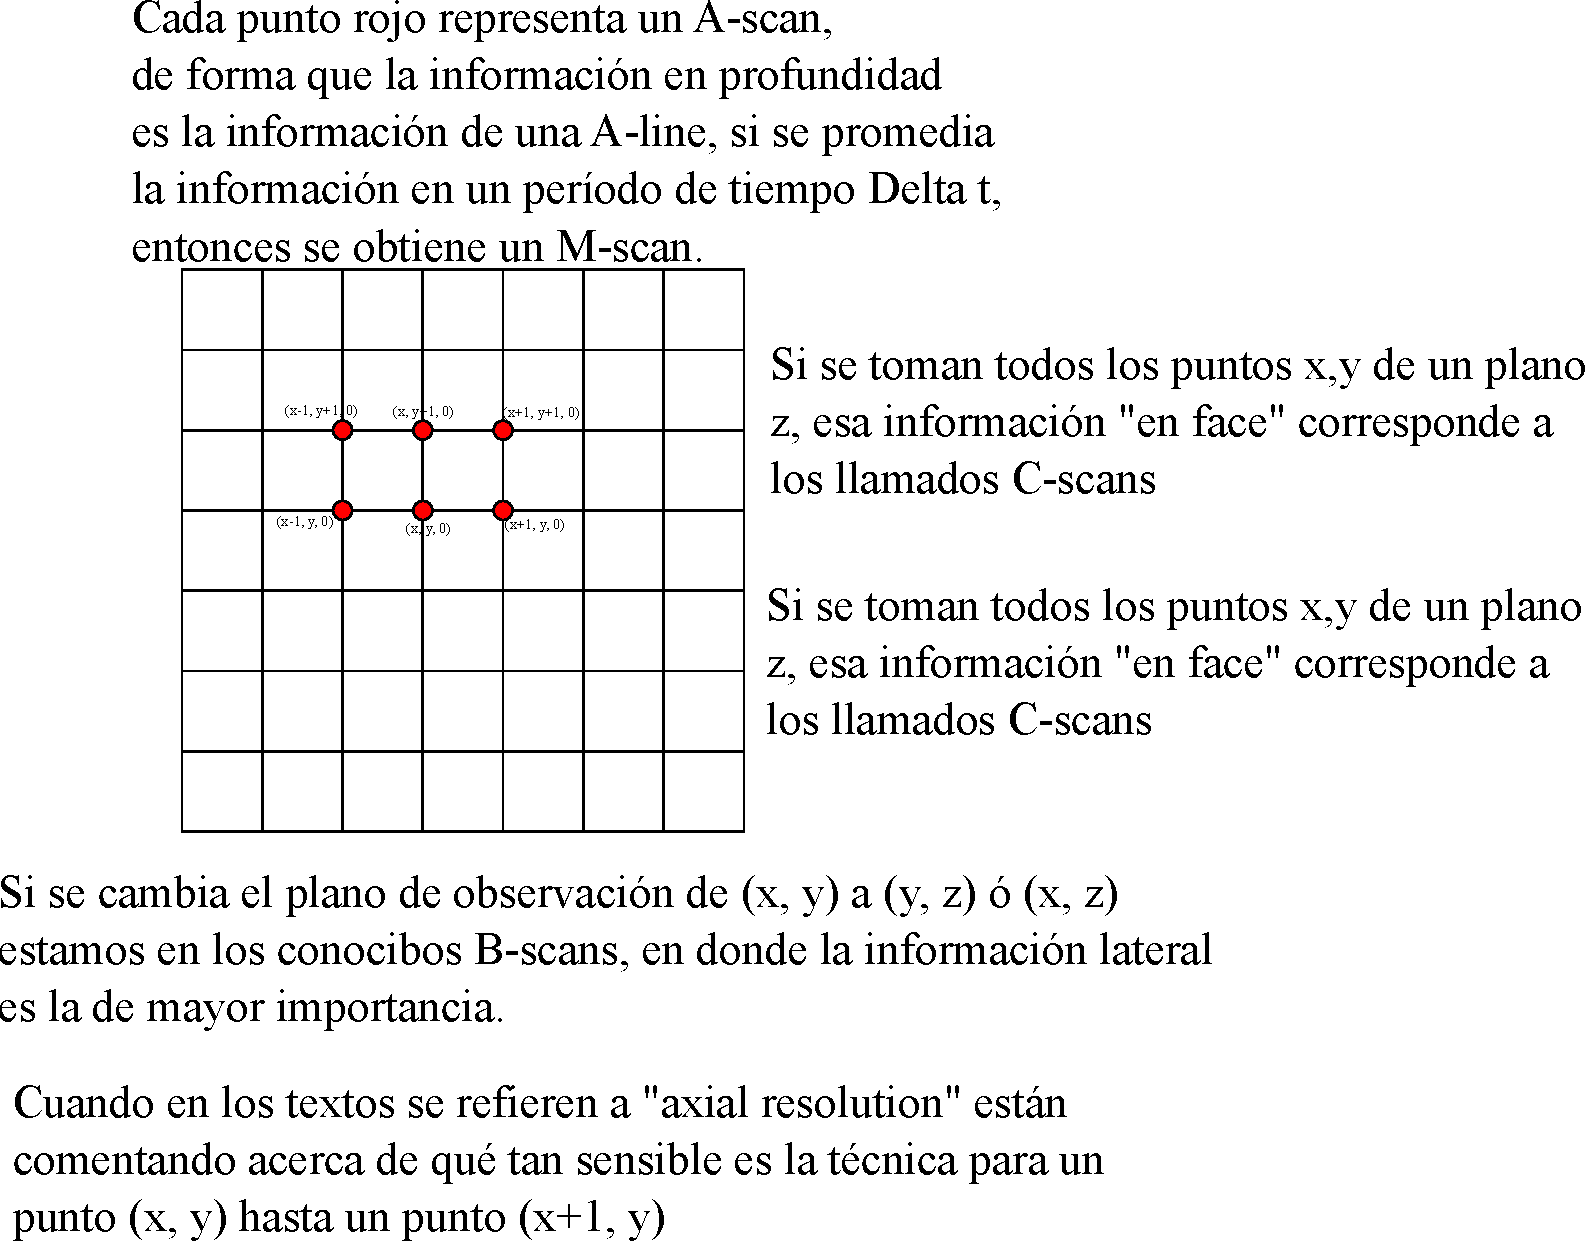
\includegraphics[width=0.7\linewidth]{img/a_scan.pdf}
%	\caption{Interpretación de la resolución axial, y los tipos de escaneos}
%	\label{fig:ascan}
%\end{figure}

%\begin{figure}
%\centering
%\includegraphics[scale=0.7]{img/gauss_reflect_oct.png}
%\caption{1}
%\label{fig:gaussreflectoct}
%\end{figure}

\subsection{Interferometría de baja coherencia en el dominio del tiempo}

%En la OCT en el dominio del tiempo TDOCT (\textit{time-domain optical coherence tomography}), el barrido no se realiza mediante el cambio del número de onda $k$, sino que a través de diferentes desplazamientos en el espejo de referencia $z_R$ se escanea la reflectividad de la muestra. En este proceso, a diferencia del caso anterior, hay una integración sobre todos los números de onda, de forma que la Eq.~\ref{eq:ID_fin} es convierte en


En OCT en el dominio del tiempo TDOCT (\textit{time-domain optical coherence tomography}) los escaneos en profundidad se realizan a través del desplazamiento del espejo de referencia, es decir, variaciones en $z_R$. La función encargada de la modulación $\cos[2k(z_R - z_{S_n})]$ aporta información en diferentes frecuencias si se varía la distancia entre el haz referencia y el haz objeto $(z_R - z_{S_n})$, o si bien se modifica el número de onda $k$, siendo ambos procesos equivalentes. Como todo el espectro llega hasta el detector, en la Eq.~\ref{eq:ID_fin} debe realizarse una integración sobre los números de onda, y el patrón de interferencia dependerá entonces de la reflectividad de la muestra y la diferencia de camino óptico. Integrando con respecto a $k$ la Eq.~\ref{eq:ID_fin} se obtiene que

\begin{align}
I_D(z_R) = &\frac{\rho}{4}S_0 [R_R+ R_{S1}+ R_{S2}+...]\\ \notag
&+\frac{\rho}{2}\left[ S_0 \sum_{n=1}^{N} \sqrt{R_R R_{S_n}} e^{-[z_R-z_{S_n}]^2 \Delta k^2}  \cos[2k_0 (z_R-z_{S_n})]\right],
\end{align}

\noindent donde $S_0$ es la potencia de la fuente ($\int_{k=0}^{\infty}S(k)dk$). En este caso, los términos que aparecen corresponden a una componente DC y una función coseno, cuya frecuencia depende de la longitud de onda central de la fuente $k_0$ y la diferencia de camino óptico entre los brazos, que se encuentra modulada por funciones gaussianas. 

Si se tienen varios reflectores se produce una señal de interferencia en sus posiciones, lo que se ha denominado línea A (A-line), esto se ejemplifica en la Fig.~\ref{fig:tdoct}, donde cuatro reflectores muestran interferencia, la señal que se desea medir corresponde justamente a la envolvente de estas funciones. La reflectividad de la muestra se puede encontrar entonces a través de la medida de la modulación que produce la señal portadora (la función coseno) sobre la función gaussiana de cada reflector, asimismo, la anchura a la mitad del máximo (FWHM:\textit{full-width at half maximum}) de cada función gaussiana está dado por la longitud de coherencia de la fuente, que es justamente la resolución axial de OCT.

\begin{figure}[h!]
	\centering
	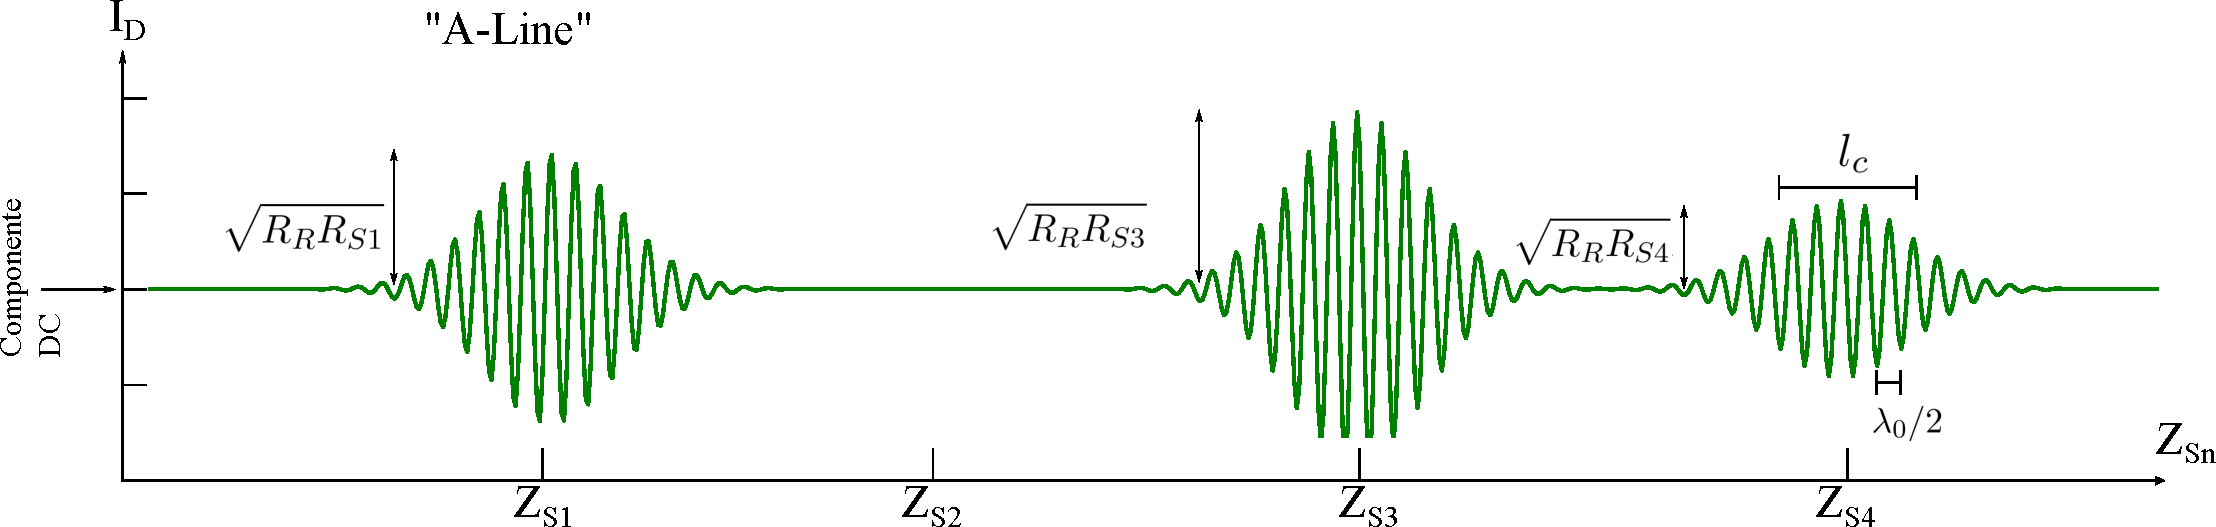
\includegraphics[width=\linewidth,keepaspectratio]{img/chap2/A_Line_1Gen}
	\caption[Línea A medida con OCT en el dominio temporal]{Línea A obtenida cuando se realiza el escaneo a una muestra con cuatro reflectores. La magnitud de la interferencia es lo que se busca medir mediante OCT.}
	\label{fig:tdoct}
\end{figure}


\subsection{Interferometría de baja coherencia en el dominio de Fourier}
\label{sec:int_baja_coh_fourier}

En OCT en el dominio de Fourier FDOCT (\textit{Fourier-domain optical coherence tomography}), la fotocorriente dependiente del número de onda $I_D(k)$ de la Eq.~\ref{eq:ID_fin} se captura y procesa mediante un análisis de Fourier que permite determinar el perfil de reflectividad $\sqrt{R_S(z_S)}$ de la muestra. En este proceso, el espejo de referencia se mantiene en una posición fija, mientras que las diferentes longitudes de onda son las encargadas de aportar la información de las diferentes profundidades en la muestra. En esta categoría hay dos divisiones para OCT, por un lado se encuentra la tomografía óptica de coherencia en el dominio espectral SDOCT (\textit{spectral-domain optical coherence tomography}) o tomografía óptica de coherencia basada en espectrómetro. OCT en el dominio espectral se basa en el empleo de una fuente de luz con banda ancha, con la diferencia de ubicar un espectrómetro en la salida del interferómetro, y todas las componentes frecuenciales de $I_D(k)$ se capturan de manera simultánea. Por otro lado, está la tomografía óptica de coherencia de fuente de barrido SSOCT (\textit{swept-source optical coherence tomography}), llamada también imagen óptica en el dominio frecuencial OFDI (\textit{optical frequency-domain imaging}). En este caso, las componentes espectrales de $I_D(k)$ se obtienen de forma secuencial, capturando la señal de una banda angosta, mientras que la fuente realiza un barrido por las diferentes longitudes de onda.

El perfil de reflectividad de la muestra $r_S(z_S)$ se calcula mediante la transformada inversa de Fourier de la corriente en el fotodetector, tomando en cuenta que la transformada de Fourier de un coseno es $\mathscr{F}\{\cos(kz_0)\} \rightleftarrows 1/2[\delta(z\pm z_0)]$ y la transformada de Fourier de la convolución es el producto de las las transformadas de Fourier de las funciones convolucionadas $x(z) \otimes y(z) \rightleftarrows X(k)Y(k)$; la transformada inversa de la Eq.~\ref{eq:ID_fin} corresponde a

\begin{align}
\label{eq:i_D_1}
i_D(z) &= \frac{\rho}{8}\left[\gamma (z) [R_R + R_{S1} + R_{S2} + ...] \right]\\ \notag
&+ \frac{\rho}{4} \left[\gamma (z) \otimes \sum_{n=1}^{N} \sqrt{R_R R_{S_n}}\{\delta[z\pm (2(z_R-z_{S_n}))]\}\right]\\
&+ \frac{\rho}{8} \left[\gamma (z) \otimes \sum_{m\neq n = 1}^{N} \sqrt{R_{s_n}R_{s_m}} \{\delta [z\pm 2(z_{S_n} - z_{S_m})]\} \right],\notag
\end{align}

\noindent donde $\gamma$ es la distribución espectral de la fuente en el plano espacial. La convolución de la función $\delta$ con la función coseno se puede calcular mediante sus propiedades, de manera que la Eq.~\ref{eq:i_D_1} corresponde a

\begin{align}
\label{eq:i_D_2}
i_D(z) &= \frac{\rho}{8}\left[\gamma (z) [R_R + R_{S1} + R_{S2} + ...] \right]\\ \notag
&+ \frac{\rho}{4} \left[\sum_{n=1}^{N} \sqrt{R_R R_{S_n}}\{\gamma [2(z_R - z_{S_n}) ] + \gamma[-2(z_R - z_{S_n}) ]\}  \right]\\
&+ \frac{\rho}{8} \left[ \sum_{m\neq n = 1}^{N} \sqrt{R_{S_n}R_{S_m}} \{\gamma [2(z_{S_n} - z_{S_m}) ] + \gamma[-2(z_{S_n} - z_{S_m}) ]\}  \right].\notag
\end{align}

\noindent La Eq.~\ref{eq:i_D_2} es una discretización de la función gaussiana correspondiente a las posiciones de los reflectores de la muestra, lo que se ha denominado línea A y se muestra en la Fig.~\ref{fig:fdoct}.
\begin{figure}[ht!]
	\centering
	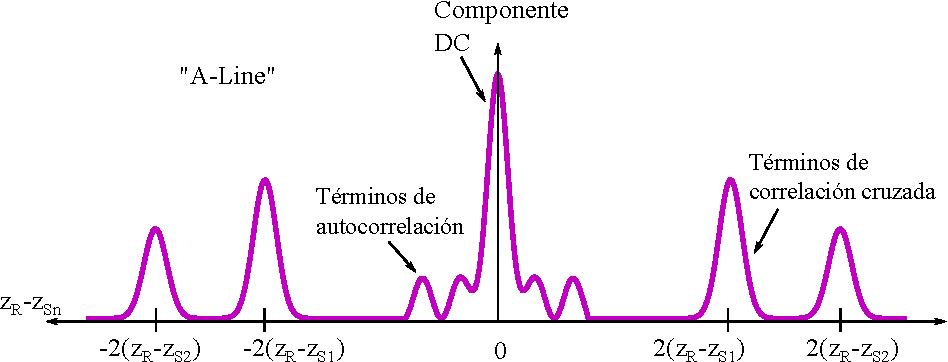
\includegraphics[width=\linewidth]{img/chap2/A_Line_FFT}
	\caption[Línea A obtenida en una medición de OCT en el dominio espectral]{Línea A obtenida en una medición de OCT en el dominio espectral. Una de las imágenes es producto de artefactos en la transformada de Fourier.}
	\label{fig:fdoct}
\end{figure}

La función que se quiere recuperar $\sqrt{R_S(z_S)}$ en este caso se reproduce con las siguientes modificaciones, primero la distancia que se mide desde la posición de referencia está duplicada. El ancho de cada función $\delta$ está dado por la longitud de coherencia de la fuente. En la Eq.~\ref{eq:i_D_1} puede apreciarse claramente la convolución entre la muestra (el objeto) y la distribución de la fuente, esta definición indica la correspondencia entre la función extendida de punto ($PSF$) en un sistema óptico convencional y la distribución espectral de la fuente. Finalmente, la aparición de la segunda función $\delta$ se debe al complejo conjugado que resulta de la transformada de Fourier de la función coseno, en general, este término representa ruido o ``artefactos'' en la información que se recupera, sin embargo, existe diferentes técnicas para solucionar este problema \cite{Ho2006,Vergnole2008}.


\section{Algunos parámetros importantes en OCT}
\label{sec:param_important}

%Aunque hay muchos parámetros de alta importancia en un montaje experimental de OCT, a continuación se mencionarán 

\subsection{Fuentes de iluminación}

Uno de los parámetros más importantes que afectan el desempeño de un equipo de OCT corresponde a la fuente de iluminación. En OCT, se busca que la fuente posea un espectro de emisión en el infrarrojo, tenga una longitud de coherencia de máximo $50nm$ y que posea una potencia mayor a $10mW$. La emisión en infrarrojo está relacionada con las características de las muestras, en donde las estructuras biológicas estudiadas por lo general tienen propiedades inhomogéneas, compuestas principalmente de colágeno y fibras elásticas, células, venas y nervios, entre otras estructuras \cite{Fercher2003}. Éstas poseen diferentes índices de absorción y esparcimiento de luz, acorde con la longitud de onda, en OCT se busca que la absorción respecto a la longitud de onda sea lo menor posible, de forma que la luz llegue hasta capas profundas en el tejido. Para alcanzar estas características se utilizan longitudes de onda mayores al visible, dado que los tejidos poseen una menor absorción en el rango de longitudes de onda de $600$ a $1300nm$ \cite{Parsa1989,Brezinski1996}. Además, como la absorción afecta la profundidad máxima en la cual se puede tener imagen, en el caso de aplicaciones en tejidos biológicos, las longitudes de onda empleadas en OCT están en el rango típico de $800$ a $1300nm$ \cite{Drexler2015}.

%Las fuentes de iluminación en OCT deben tener una baja coherencia. En este sentido, se denomina fuente coherente a aquella que produce una relación fija de fase entre los valores del campo en diferentes ubicaciones o en distintos instantes, es decir, que la fase que posee un punto en el espacio y en el tiempo mantenga una relación fija con la fase. Se definen entonces dos tipos de coherencia: espacial y temporal. La coherencia espacial ocurre cuando hay una correlación entre la fase en diferentes puntos del espacio a lo largo del perfil del haz. En OCT no hay mucha coherencia espacial, pues la presencia de esta incrementa la relación señal ruido, ya que entre mayor coherencia espacial, más profundidades a lo largo de la muestra generan intereferencia, y esto se refleja como moteado (ruido multiplicativo \textit{speckle}). La coherencia espacial se da cuando hay correlación en un punto determinado del perfil del haz a lo largo del tiempo. Esta coherencia es dictada por la fuente, y es la encargada de determinar la resolución axial del sistema de OCT. Fuentes con un menor tiempo de coherencia, y por tanto, anchos espectrales más grande, producen una mayor resolución axial; mientras que fuentes con un menor tiempo de coherencia produce resoluciones axiales más bajas. Respecto a la distribución del espectro, en general en OCT, las fuentes poseen un espectro gaussiano a sus propiedades. Sin embargo, se puede emplear fuentes con distribuciones no gaussianas, pero la calidad de las líneas A obtenidas es, en la mayor parte de los casos, de una peor calidad. Eso es causado por la aparición de sombras en el interferograma capturado \cite{Jansz2012}. 

Las fuentes de iluminación en OCT deben tener una baja coherencia. En este sentido, se denomina fuente coherente a aquella que produce una relación fija de fase en el campo complejo en diferentes ubicaciones o en distintos instantes, es decir, la fase de un haz coherente debe mantenerse constante en el espacio y el tiempo en cualquier punto en el perfil del haz \cite{Born1983}. Se definen entonces dos tipos de coherencia: espacial y temporal. La coherencia espacial ocurre cuando hay una correlación de la fase en diferentes puntos del espacio a lo largo del perfil del haz \cite{Hecht2000}. En OCT no hay mucha coherencia espacial pues la presencia de ésta decrementa la relación señal ruido, puesto que a mayor coherencia espacial más profundidades a lo largo de la muestra generan interferencia, y esto se refleja como patrones de interferencia aleatorios indeseados o \textit{speckle} \cite{Drexler2015}. La coherencia temporal por otro lado, se da cuando hay correlación en un punto determinado del perfil del haz a lo largo del tiempo \cite{Hecht2000}. Esta coherencia es dictada esencialmente por la distribución espectral de la fuente, y es la encargada de determinar la resolución axial del sistema de OCT \cite{Brezinski2005}. Fuentes con un menor tiempo de coherencia, y por tanto, anchos espectrales más grande, producen una mayor resolución axial; mientras que fuentes con un menor tiempo de coherencia produce resoluciones axiales más bajas, ya que hay una dependencia entre el ancho espectral y la resolución axial del sistema \cite{Brezinski2005}. Por último, respecto a la distribución del espectro, en general, las fuentes poseen un espectro gaussiano gracias a sus propiedades \cite{Brezinski2005}. Sin embargo, se pueden emplear fuentes con distribuciones no gaussianas, pero la calidad de las imágenes obtenidas, es peor en la mayor parte de los casos, a causa de la aparición de sombras y artefactos en el patrón de interferencia capturado \cite{Jansz2012}. 

%Entre las fuentes de luz más comunes para OCT, se encuentran los diodos superluminiscentes (SLDs)\cite{Ko2004}, los láseres de estado sólido \cite{Drexler1999} y las fuentes de barrido \cite{Choma2003}. Los diodos superluminiscentes funcionan a partir de una unión p-n directamente polarizada, inyectando eléctrones y huecos en las zonas p y n respectivamente. La carga correspondiente a los portadores minoritarios inyectados en cada una de estas zonas se recombina con la correspondiente a la de los portadores mayoritarios en la zona de agotamiento o en las zonas neutras. En semiconductores de gap directo, esta recombinación da lugar a una emisión de fotones. La principal ventaja que tiene, es su relativo bajo costo y espectro gaussiano; la resolución axial para estos elementos, se encuentra en el orden de los $16\mu m$ en tejido, y las longitudes de onda centrales están entre los $700$ y $1550nm$. Los láseres de estado sólido, se basan en un medio cristalino, dopados con iones en puntos específicos de la red cristalina, esta modificación permite diferentes posibilidades para la longitud de onda de excitación y por tanto de emisión. Con láseres de Titanio-Safiro, comúnes en OCT, la resolución axial puede llegar hasta $1\mu m$ en tejido. Las fuentes de barrido, emiten luz en un espectro angosto, cambiando rápidamente a lo largo del rango espectral de la fuente, obteniéndose una longitud de onda cambiante, este tipo de fuente alcanza resoluciones de hasta $1\mu m$, a tasas de adquisión de $1kHz$.

Entre las fuentes de luz más comunes para OCT, se encuentran los diodos superluminiscentes (SLDs)\cite{Ko2004}, los láseres de estado sólido \cite{Drexler1999} y las fuentes de barrido \cite{Choma2003}. Los diodos superluminiscentes funcionan a partir de una unión p-n directamente polarizada, inyectando electrones y huecos en las zonas p y n respectivamente, la recombinación luego de las inyecciones da lugar a una emisión de fotones. La principal ventaja que tiene, es su relativo bajo costo y espectro gaussiano; la resolución axial para estos elementos, se encuentra en el orden de los $16\mu m$ en tejido, y las longitudes de onda centrales están entre los $700$ y $1550nm$ \cite{Ko2004}. Los láseres de estado sólido, se basan en un medio cristalino, dopados con iones en puntos específicos de la red cristalina, esta modificación permite diferentes posibilidades para la longitud de onda de excitación y por tanto de emisión. Con láseres de Titanio-Safiro, comunes en OCT, la resolución axial puede llegar hasta $1\mu m$ en tejido \cite{Drexler1999}. Las fuentes de barrido emiten luz en un espectro angosto, cambiando rápidamente a lo largo del rango espectral de la fuente, obteniéndose una longitud de onda cambiante, este tipo de fuente alcanza resoluciones de hasta $1\mu m$, a tasas de adquisición de $1kHz$ \cite{Choma2003}.

\subsection{Resolución axial y lateral}

La resolución en OCT se define mediante dos parámetros, la resolución axial o de profundidad y la resolución lateral o transversal. Una de las características de OCT con respecto a la microscopía, es que la resolución lateral y axial corresponden a parámetros diferentes. La resolución axial $\Delta z$, es dependiente de la distribución espectral de la fuente, para un espectro gaussiano cuya longitud de onda central sea $\lambda_0$ y su anchura a la mitad del máximo ($FWHM$) $\Delta \lambda$, corresponde a \cite{Brezinski2005}

\begin{equation}
\Delta z = \frac{2 \ln 2}{\pi} \frac{\lambda_0^2}{\Delta \lambda}.
\end{equation}

La resolución lateral funciona de manera similar a la microscopía, ya que la determina las propiedades del haz enfocado, correspondiente al mínimo tamaño del haz; y es inversamente proporcional a la apertura numérica ($NA$) de la lente de enfoque. De manera similar a la microscopía confocal, la resolución lateral $\Delta x$ en OCT se define como \cite{Drexler2015}
\begin{equation}
\Delta x  = \frac{4\lambda_0}{\pi} \left( \frac{f}{D}\right) = \frac{4\lambda_0}{\pi NA},
\end{equation}
\noindent donde $f$ es la distancia focal efectiva de la lente y $D$ es el tamaño del haz proyectado en la lente de enfoque. La región de enfoque del haz, conocida como profundidad de foco $b$ (el doble del rango de Rayleigh $z_R$), se define como

\begin{equation}
\label{eq:depth_of_focus}
	b = 2z_R = \frac{\pi \Delta x^2}{2\lambda_0}.
\end{equation}

Aunque la resolución axial y transversal son independientes, la capacidad de penetración de OCT también varía con la apertura numérica, una mayor $NA$ incrementa la resolución lateral, pero disminuye la profundidad de foco, mientras que una menor $NA$ produce una menor resolución lateral, pero incrementa el rango de escaneo. En general, OCT emplea aperturas numéricas bajas para incrementar la profundidad de penetración, en el caso de altas resoluciones transversales, existen otras técnicas derivadas de OCT como la microscopía óptica de coherencia (OCM: \textit{optical coherence microscopy}) \cite{Beaurepaire1998}.

\subsection{Sensibilidad}

La sensibilidad es una medida de la mínima reflectividad de la muestra  $R_{S, min}$ detectable por el sistema, se obtiene en el nivel al cual la relación señal ruido se convierte en uno. Expresado en unidades de decibelios, la sensibilidad $S_{dB}$ corresponde a \cite{Drexler2015}

\begin{equation}
S_{dB} = 10\log_{10} \left(\frac{1}{R_{S,min}}\right)
\end{equation}
En un sistema de OCT, $S_{dB}$ puede medirse experimentalmente ubicando filtros de densidad neutra conocida en el brazo objeto y posteriormente un espejo. Considerando que la luz atraviesa dos veces el filtro, la sensibilidad puede obtenerse cuando la señal proveniente de la muestra sea indistinguible del ruido. Los valores típicos de sensibilidad para sistemas de OCT se encuentra en el rango de los $-95dB$ ($R_{S, min}=3.16\times 10^{-10}$ veces la luz incidente) \cite{Drexler2015}. 

La capacidad para generar imágenes en profundidad de un sistema de OCT depende de la sensibilidad que éste posea, y es quien dicta la capacidad para producir imágenes de estructuras debajo de las capas superficiales. La señal de OCT sufre un decaimiento (\textit{roll-off}) exponencial con la profundidad \cite{Fercher2003, Drexler2015}, esta perdida en la señal se debe a varios motivos: el espectro finito de la fuente que limita la distancia máxima sobre la cual puede obtenerse interferencia, asimismo, la frecuencia que posee el patrón de franjas detectado incrementa con la diferencia de camino óptico, a su vez relacionado con la profundidad de penetración. En escala logarítmica, el decaimiento de la señal con respecto a la profundidad de un sistema de OCT no debe tener un valor de más de $10dB/mm$, aunque esto dependerá del medio y de las propiedades de la fuente \cite{Drexler2015}.

\subsection{Relación señal ruido}
\label{subsec:SNR}

La relación señal ruido ($SNR$: \textit{signal-to-noise ratio}) refiere al nivel de la señal que transporta información relevante, con respecto a las variaciones aleatorias y el ruido de fondo que posee el instrumento o sistema de medida. La relación señal ruido, se define como el cociente entre la intensidad media en el detector $\bar{I}_d$, con respecto a la varianza de ruido $\sigma_n$ \cite{Rollins1999_2},

\begin{equation}
\label{eq:SNR}
	SNR = \frac{\bar{I}_d}{\sigma_n},
\end{equation}

\noindent o expresado de manera logarítmica,

\begin{equation}
	SNR = 10\log_{10}\left( \frac{\bar{I}_d}{\sigma_n}\right).
\end{equation}

%La intensidad detectada en el sensor $I_d$ corresponde a
%
%\begin{equation}
%I_d = \rho \left(P_s+P_x+2\sqrt{P_xP_s}\cos(k_0\Delta z)\right),
%\end{equation}


%La relación señal ruido ($SNR$: \textit{signal-to-noise ratio}) refiere al nivel de la señal que transporta información relevante, con respecto a las variaciones aleatorias y el ruido de fondo que posee el instrumento o sistema de medida. La relación señal ruido, se define como el cociente entre la intensidad de la señal a medir $P_s$, con respecto a la señal de ruido $P_n$,
%
%\begin{equation}
%\label{eq:SNR}
%SNR = \frac{P_s}{P_n},
%\end{equation}
%
%\noindent o expresado de manera logarítmica,
%
%\begin{equation}
%SNR = 10\log_{10}\left( \frac{P_s}{P_n}\right).
%\end{equation}
%
%La intensidad detectada en el sensor $I_d$ corresponde a
%
%\begin{equation}
%I_d = \rho \left(P_s+P_x+2\sqrt{P_xP_s}\cos(k_0\Delta z)\right),
%\end{equation}

%La intensidad de la señal, puede describirse como el promedio del cuadrado de la señal en el detector $\langle i_d^2 \rangle$,

%\begin{equation}
%\langle i_d^2 \rangle = 2\rho P_r P_s ,
%\end{equation}

%\noindent donde $\rho$ corresponde al factor de respuesta del detector, $P_r$ es la potencia reflejada por el haz de referencia y $P_s$ es la potencia del haz reflejado por la muestra. Si el ruido tiene una varianza $\sigma^2_{nse}$, el $SNR$ puede definirse como

%\begin{equation}
%SNR_{dB} = 10\log_{10}\left(\frac{\langle i_d^2 %\rangle}{\sigma_{nse}^2}\right).
%\end{equation}

Aunque existen diferentes fuentes de ruido, en esta sección, se describirán tres de las más importantes, ruido de disparo (\textit{shot noise}), ruido térmico y ruido causado por exceso de fotones; otras causas de ruido tales como el \textit{speckle} serán discutidas en el Capítulo \ref{chapter:supresion_ruido_en_oct}.

\subsubsection{Ruido de disparo}

%El ruido de disparo corresponde a las fluctuaciones producidas por la cantidad de fotones con las que se produce la fotocorriente en el detector. El movimiento de cargas para generar la corriente depende de la intensidad media en el detector, pero el instante en el que la fotocorriente se emite es aleatorio, esto permite que el tiempo de llegada de un fotón hasta el detector, y el tiempo de emisión de la fotocorriente puedan describirse mediante una distribución de Poisson. La varianza en la fotocorriente $i_s$ a partir de dicha distribución corresponde a

El ruido de disparo corresponde a las fluctuaciones causadas por la cantidad de fotones con los que se produce la fotocorriente en el detector. La corriente de respuesta del detector, está determinada por el promedio del conteo de fotones incidentes sobre el sensor, en periodos de tiempo fijos. No obstante, la cantidad de fotones incidentes en el detector no siempre es la misma, y por tanto, la fotocorriente inducida no es constante, a estas variaciones en la señal originadas por el promedio de fotones incidentes en el detector, se le conoce como ruido de disparo \cite{Tomlins}. La varianza en la fotocorriente $i_s^2$ a partir de dicho ruido corresponde a \cite{Rollins1999_2}
\begin{equation}
	i_s^2=2 e \bar{I}_d \Delta f,
\end{equation}
donde $e$ es la carga del electrón, $\bar{I}_d$ es la fotocorriente media en el detector y $\Delta f$ es el ancho de banda del detector.

\subsubsection{Ruido térmico}

El ruido térmico se debe principalmente al movimiento de cargas causado por la energía térmica en cualquier elemento resistivo. Está relacionado con el equilibrio térmico y la transferencia de energía entre un material y su entorno \cite{Bouma2002}. La varianza del ruido térmico $i_t^2$, se describe como

\begin{equation}
	i_t^2 = \frac{4k_B T \Delta f}{R},
\end{equation}

\noindent donde $k_B$ es la constante de Boltzmann, $T$ es la temperatura, $\Delta f$ el ancho de banda del detector y $R$ la resistencia del material.

\subsubsection{Ruido por exceso de fotones}

El ruido por exceso de fotones surge por las fluctuaciones en la intensidad de salida de la fuente de luz, causadas por la emisión de fotones de regiones del espectro distinto a la esperada, y que poseen una fase aleatoria \cite{Rollins1999_2}. La varianza del ruido por exceso de fotones $i^2_{e}$ se indica como

\begin{equation}
i^2_{e} = \frac{(1+\alpha^2)\bar{I}_d\Delta f}{\Delta \nu},
\end{equation}

\noindent donde $\alpha$ corresponde al grado de polarización de la fuente, $\bar{I}_d$ es la corriente promedio en el detector, $\Delta f$ es el ancho espectral de la fuente y $\Delta \nu$ es el ancho efectivo de la línea. Este tipo de ruido es particularmente importante cuando se emplean fuentes de barrido.

\section{Implementación de un sistema de OCT a nivel del laboratorio}
\label{sec:impementacion}

Como se mencionó anteriormente, en su primera etapa, OCT se basó en el empleo de un interferómetro de Michelson con una fuente de luz blanca. En el laboratorio del Grupo de Óptica Aplicada, se implementó un montaje experimental de OCT que se basa en interferometría de luz blanca, empleando un desplazador piezoeléctrico para realizar escaneos axiales en la muestra. El objetivo final de este montaje, más allá de obtener imágenes \invivo que se encuentran reguladas por normas nacionales e internacionales, es obtener más claridad sobre los procedimientos, conceptos y desafíos que acarrea consigo la producción de equipos empleados en OCT. Existen diferentes aplicaciones no clínicas de OCT, tales como reconstrucción de topografía en materiales metálicos \cite{Chang2008}, en donde la componente de reflexión especular es los suficientemente intensa como para producir interferencia; o algunos especímenes biológicos \exvivo como insectos que son relativamente fáciles de analizar \cite{Molly2012}. Se espera entonces obtener resultados comparables con los obtenidos por Chang \etal \cite{Chang2008}, en la reconstrucción de la topografía de una moneda a partir de OCT; y los resultados obtenidos por Molly \etal \cite{Molly2012}, en el análisis de un insecto \textit{ex-vivo}, aunque en nuestro caso, nos centraremos en el ala de un insecto de la familia \emph{blattodea}.



%para especímenes \exvivo y como ejercicio académico para comprender los principios y funcionamiento de OCT. Con el montaje obtenido, se analizaron de manera exitosa dos muestras, una moneda, con la cual se realizó la reconstrucción de su topografía, y un ala de  (familia de las cucarachas).

%Cuando se emplea una cámara que captura los patrones de interferencia de manera directa, sobre los ejes $xy$, corresponde a OCT de campo completo (FFOCT: \textit{full-field optical coherence tomography}), y es la base sobre la cual se trabaja la microscopía óptica de coherencia, y se empleará esta técnica con los elementos disponibles en el laboratorio. 

\subsection{Componentes y descripción del montaje}

A partir de la configuración típica de un interferómetro de Michelson, se implementó el sistema óptico que se presenta en el esquema de la Fig.~\ref{fig:montajescheme}; y lo conforman las siguientes componentes con su respectiva referencia. La fuente es una lámpara halógena de tungsteno (THORLABS OSL2), cuyo espectro se muestra en la Fig.~\ref{subfig:srcspectrum}. La luz emitida por la fuente se propaga a través de una fibra óptica hasta llegar a un colimador que se encargan de reducir la alta divergencia del haz. Justo a la salida del colimador, a $1cm$, se ubica un diafragma que determina el diámetro del haz que se propagará a lo largo del sistema óptico. Este diafragma cumple también la función de aportar coherencia espacial al haz cuando la apertura se encuentra poco abierta. Luego del diafragma a $12.5cm$, se posiciona una lente (THORLABS LA1050) de $\phi=2"$ con distancia focal efectiva de $100mm$ que colecta la luz divergente después del diafragma. A continuación, se redirige el haz incidente hacia un filtro de color mediante un espejo. El filtro de color (PHYWE 8406), se encarga de tomar una porción reducida del espectro de la fuente [Fig.~\ref{subfig:srcspectrum}], absorbiendo las longitudes de onda que se encuentren por debajo de $\approx600nm$, aportando coherencia temporal al haz incidente. Después de pasar por el filtro, el espectro de la fuente se modifica al que se muestra en la Fig.~\ref{subfig:filtspectrum}, en donde la resolución axial disminuye a $2.14 \mu m$, esta corresponde a la resolución axial empleada para las mediciones. 
\begin{figure}[ht!]
	\centering
	\includegraphics[width=0.8\linewidth]{img/chap2/Montaje_scheme}
	\caption[Esquema del montaje.]{Esquema del montaje implementado.}
	\label{fig:montajescheme}
\end{figure}

\begin{figure}[ht!]
	\centering
	\subfigure[Espectro de la fuente.]{\label{subfig:srcspectrum}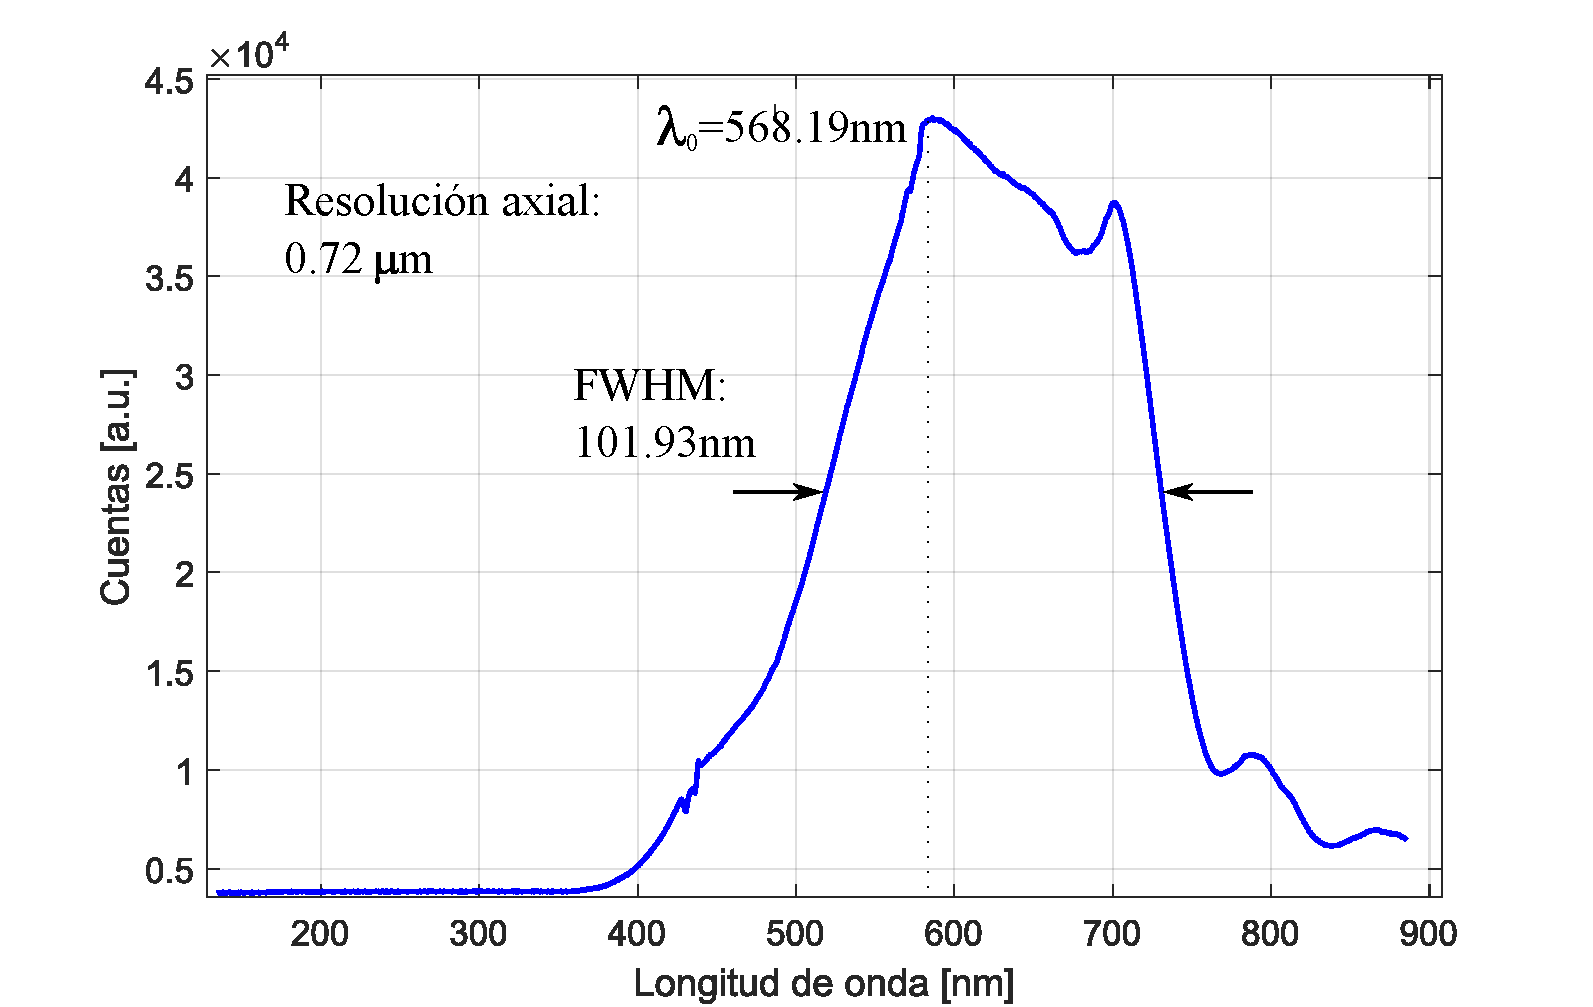
\includegraphics[width=0.49\linewidth]{img/chap2/src_spectrum}}
	\subfigure[Espectro de la fuente con filtro.]{\label{subfig:filtspectrum}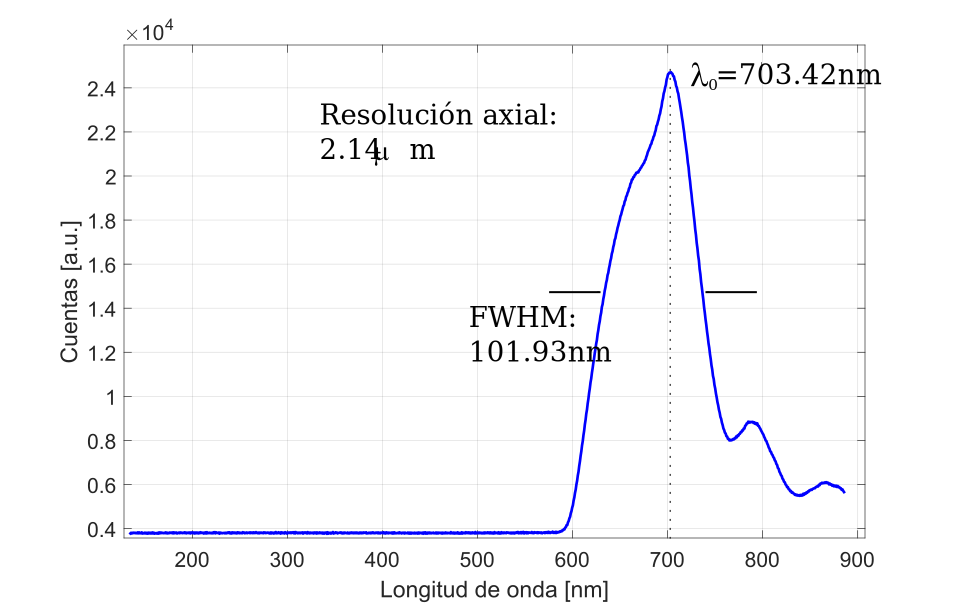
\includegraphics[width=0.49\linewidth]{img/chap2/filt_spectrum}}
	\caption[Espectro de la fuente empleada]{Espectros de la fuente halógena de tungsteno, en (a) la resolución axial es de $0.72\mu m$, mientras que en (b) corresponde a $2.14\mu m$.}
	\label{fig:spectrums}
\end{figure}

Una vez el haz ha pasado el filtro, se ubica una segunda lente (THORLABS AC254-200-A-ML) de $\phi=1"$ y distancia focal efectiva de $300mm$, con un espaciado de $5cm$ respecto a la lente, que permite enfocar el haz en la muestra, en caso de ser necesaria una mayor cantidad de luz en un área menor de la muestra. Posterior a la segunda lente, hay un cubo divisor de haz (Edmund Optics 32-702) que refleja $50\% $ de la luz incidente y transmite $50\%$. El haz transmitido, por su parte, se propaga hasta llegar a la muestra, mientras que el haz reflejado llega hasta el espejo de referencia acoplado a un desplazador piezoeléctrico (THORLABS MDT693A). El piezoeléctrico posee una resolución de $26.66nm$ por voltio y un desplazamiento máximo de $20\mu m$, éste se encuentra unido a una mesa de desplazamiento micrométrico con una resolución de $10\mu m$ y un desplazamiento máximo de $1.5cm$ para poder encontrar la región de interferencia entre los haces. Los haces reflejados vuelven al cubo divisor y pasan por una tercera lente (THORLABS LA1050) de $\phi=2"$ con distancia focal efectiva de $100mm$, que se encarga de formar imagen. El sistema formador de imagen es un $2f$, de manera que la distancia entre la lente, el espejo de referencia y la muestra es de $200mm$. Por último, en el plano imagen a $200mm$ de la última lente, se ubica una cámara CCD (Point Grey Grasshopper3 GS3-U3-91S6M-C) de $14$ bits de profundidad, resolución $3376x2704$ píxeles, tamaño de pixel $3.69\mu m$ y tasa de adquisición de datos de $9$ imágenes por segundo. Una fotografía del montaje final se presenta en la Fig.~\ref{fig:montaje}.

\begin{figure}[h!]
	\centering
	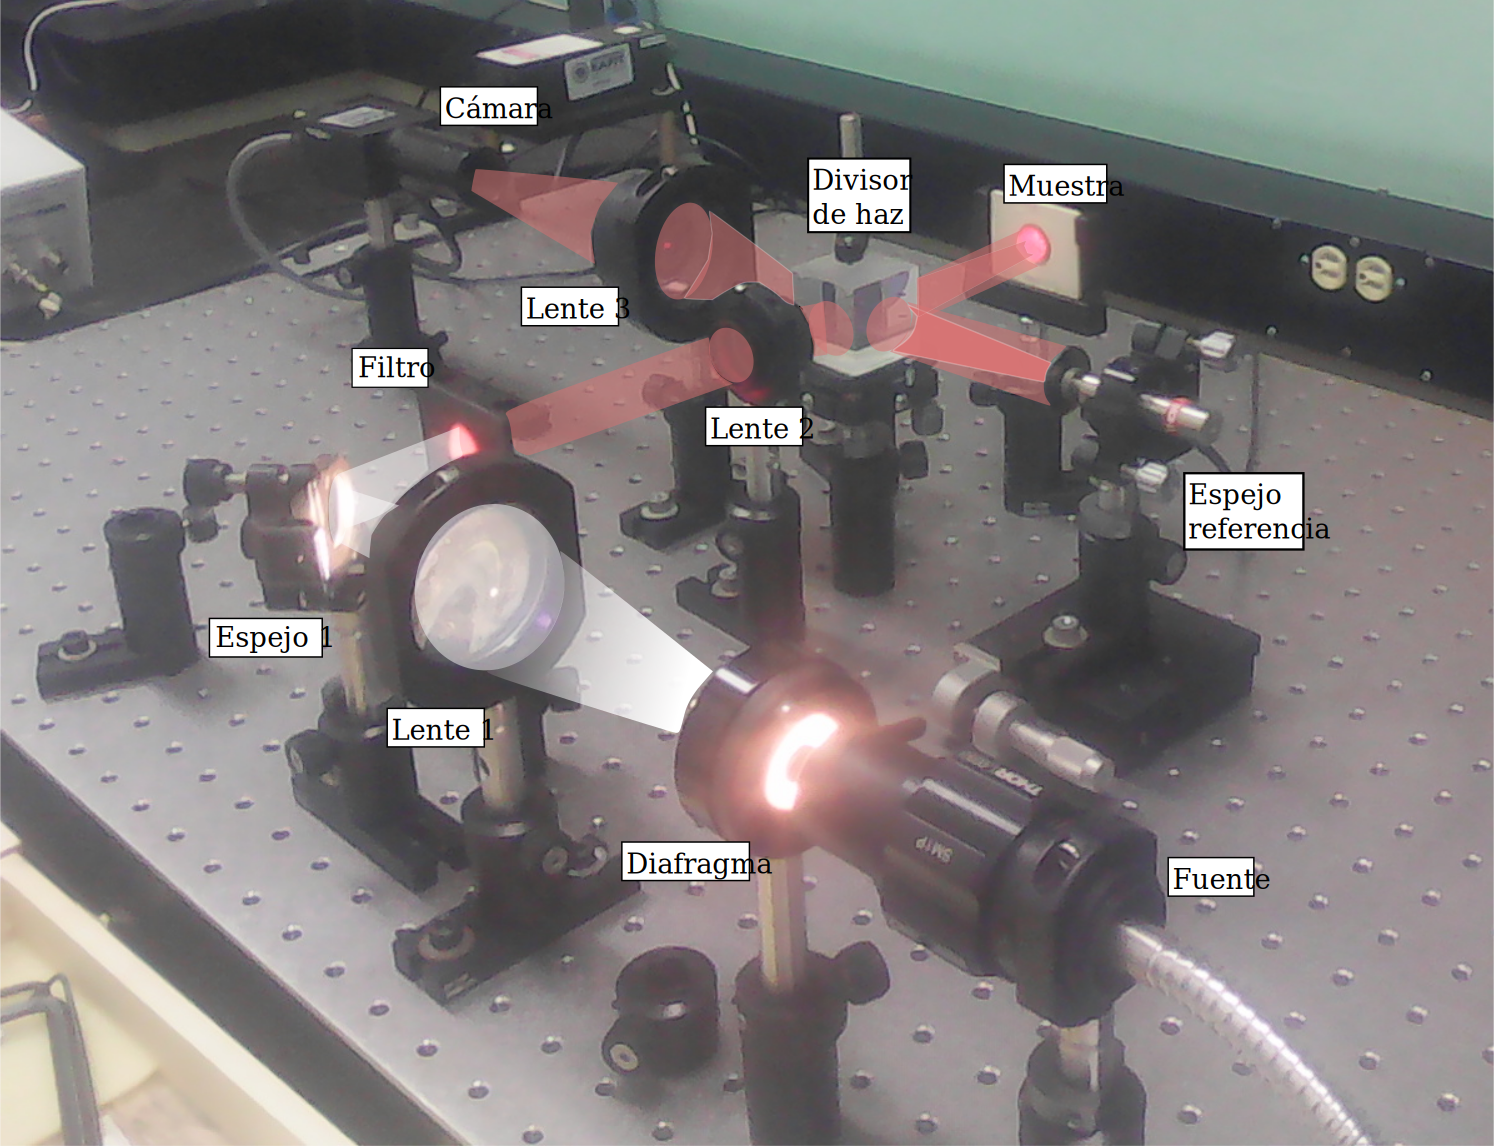
\includegraphics[width=0.8\linewidth]{img/chap2/Montaje}
	\caption[Fotografía del montaje.]{Fotografía del montaje.}
	\label{fig:montaje}
\end{figure}

\subsection{Captura de los patrones de interferencia}

La interferencia en el sistema de OCT se da unicamente cuando la diferencia de camino óptico entre el haz objeto y el haz referencia se encuentra dentro la longitud de coherencia. En el montaje implementado, ésta corresponde a $2.14\mu m$, es decir, que si la distancia recorrida por los haces que interfieren es menor que dicho rango, aparecerá un patrón de interferencia. Cuando esta distancia se obtiene, se registra el patrón que se muestra en la Fig.~\ref{subfig:patroninterferencia}. En este caso, ambos brazos poseen espejos y como el divisor de haz tiene una relación $50/50$, se espera que la interferencia sea máxima. La imagen mostrada en la Fig.~\ref{subfig:patroninterferencia} corresponde a una captura frontal del patrón, conocida en OCT como \textit{en-face}, debido a que muestra el plano $XY$ de los datos. Esta características es la base de los sistemas que emplean cámaras para capturar los patrones de interferencia, y es conocida como OCT de campo completo (FFOCT: \textit{full-field optical coherence tomography}). Como la reflectividad de la muestra se encuentra implicita en la modulación del patrón de interferencia, es necesario obtenerla mediante algoritmos similares a los de recuperación de fase, por ejemplo a partir del algoritmo de cuatro pasos \cite{Malacara1992}. En nuestro caso, se optó por emplear el algoritmo conocido como salto de fase iterativo (IPS: \textit{iterative phase shifting}) \cite{Wang2004}, este algoritmo funciona de manera similar al de cuatro pasos, pero encuentra la fase y los saltos de fase entre los interferogramas de manera iterativa, mediante un procedimiento de mínimos cuadrados. El IPS requiere al menos tres imágenes con diferentes saltos de fase, pero no requiere ninguna relación fija en los saltos de fase entre los interferogramas. Al ser un algoritmo iterativo, la precisión de la fase depende del número de iteraciones, la tolerancia del error en la función obtenida, la cantidad de imágenes que se empleen y la semilla. Empleando el IPS, con cuatro imágenes y un cambio entre iteraciones mínimo de $10^{-6}$ se obtuvo la modulación del patrón de franjas con luz blanca que se muestra en la Fig.~\ref{subfig:modulacion} en $24$ iteraciones.

\begin{figure}[ht!]
	\centering
	\subfigure[Patrón de interferencia con luz blanca.]{\label{subfig:patroninterferencia}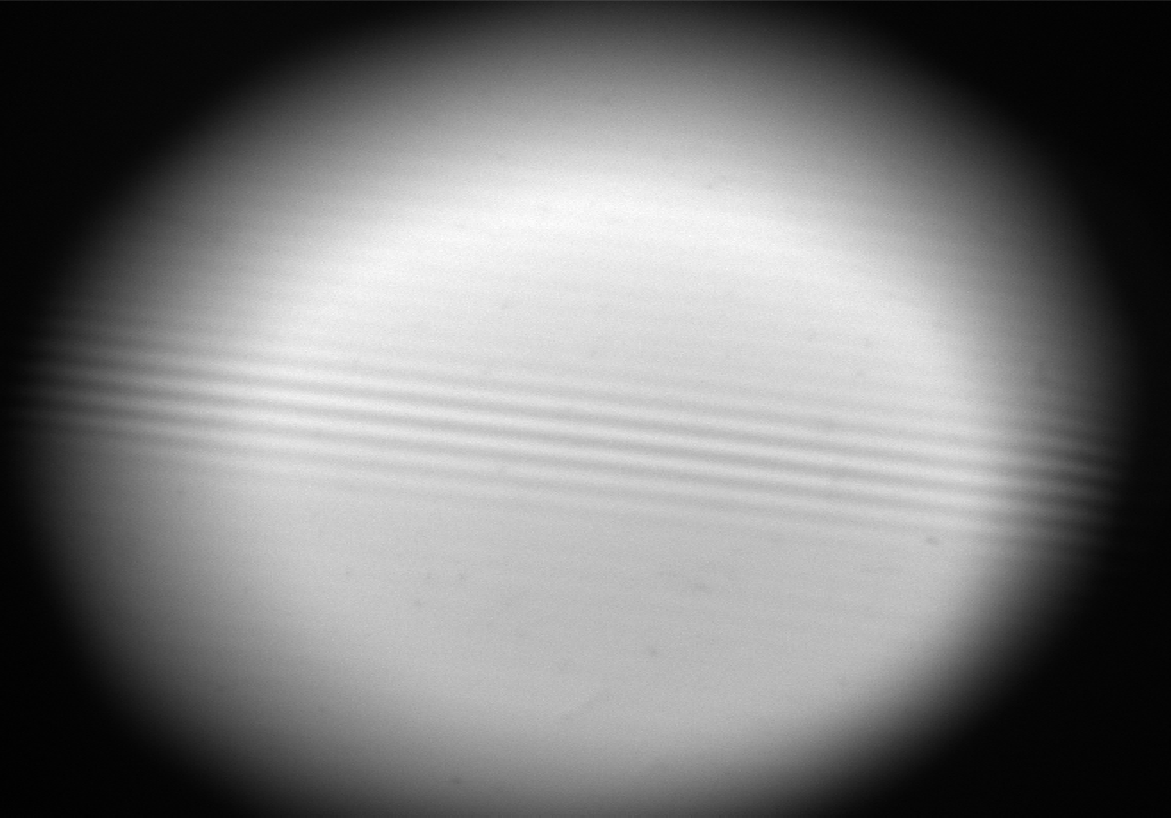
\includegraphics[width=0.49\linewidth]{img/chap2/PatronInterferencia}}
	\subfigure[Modulación en el patrón de interferencia con luz blanca.]{\label{subfig:modulacion}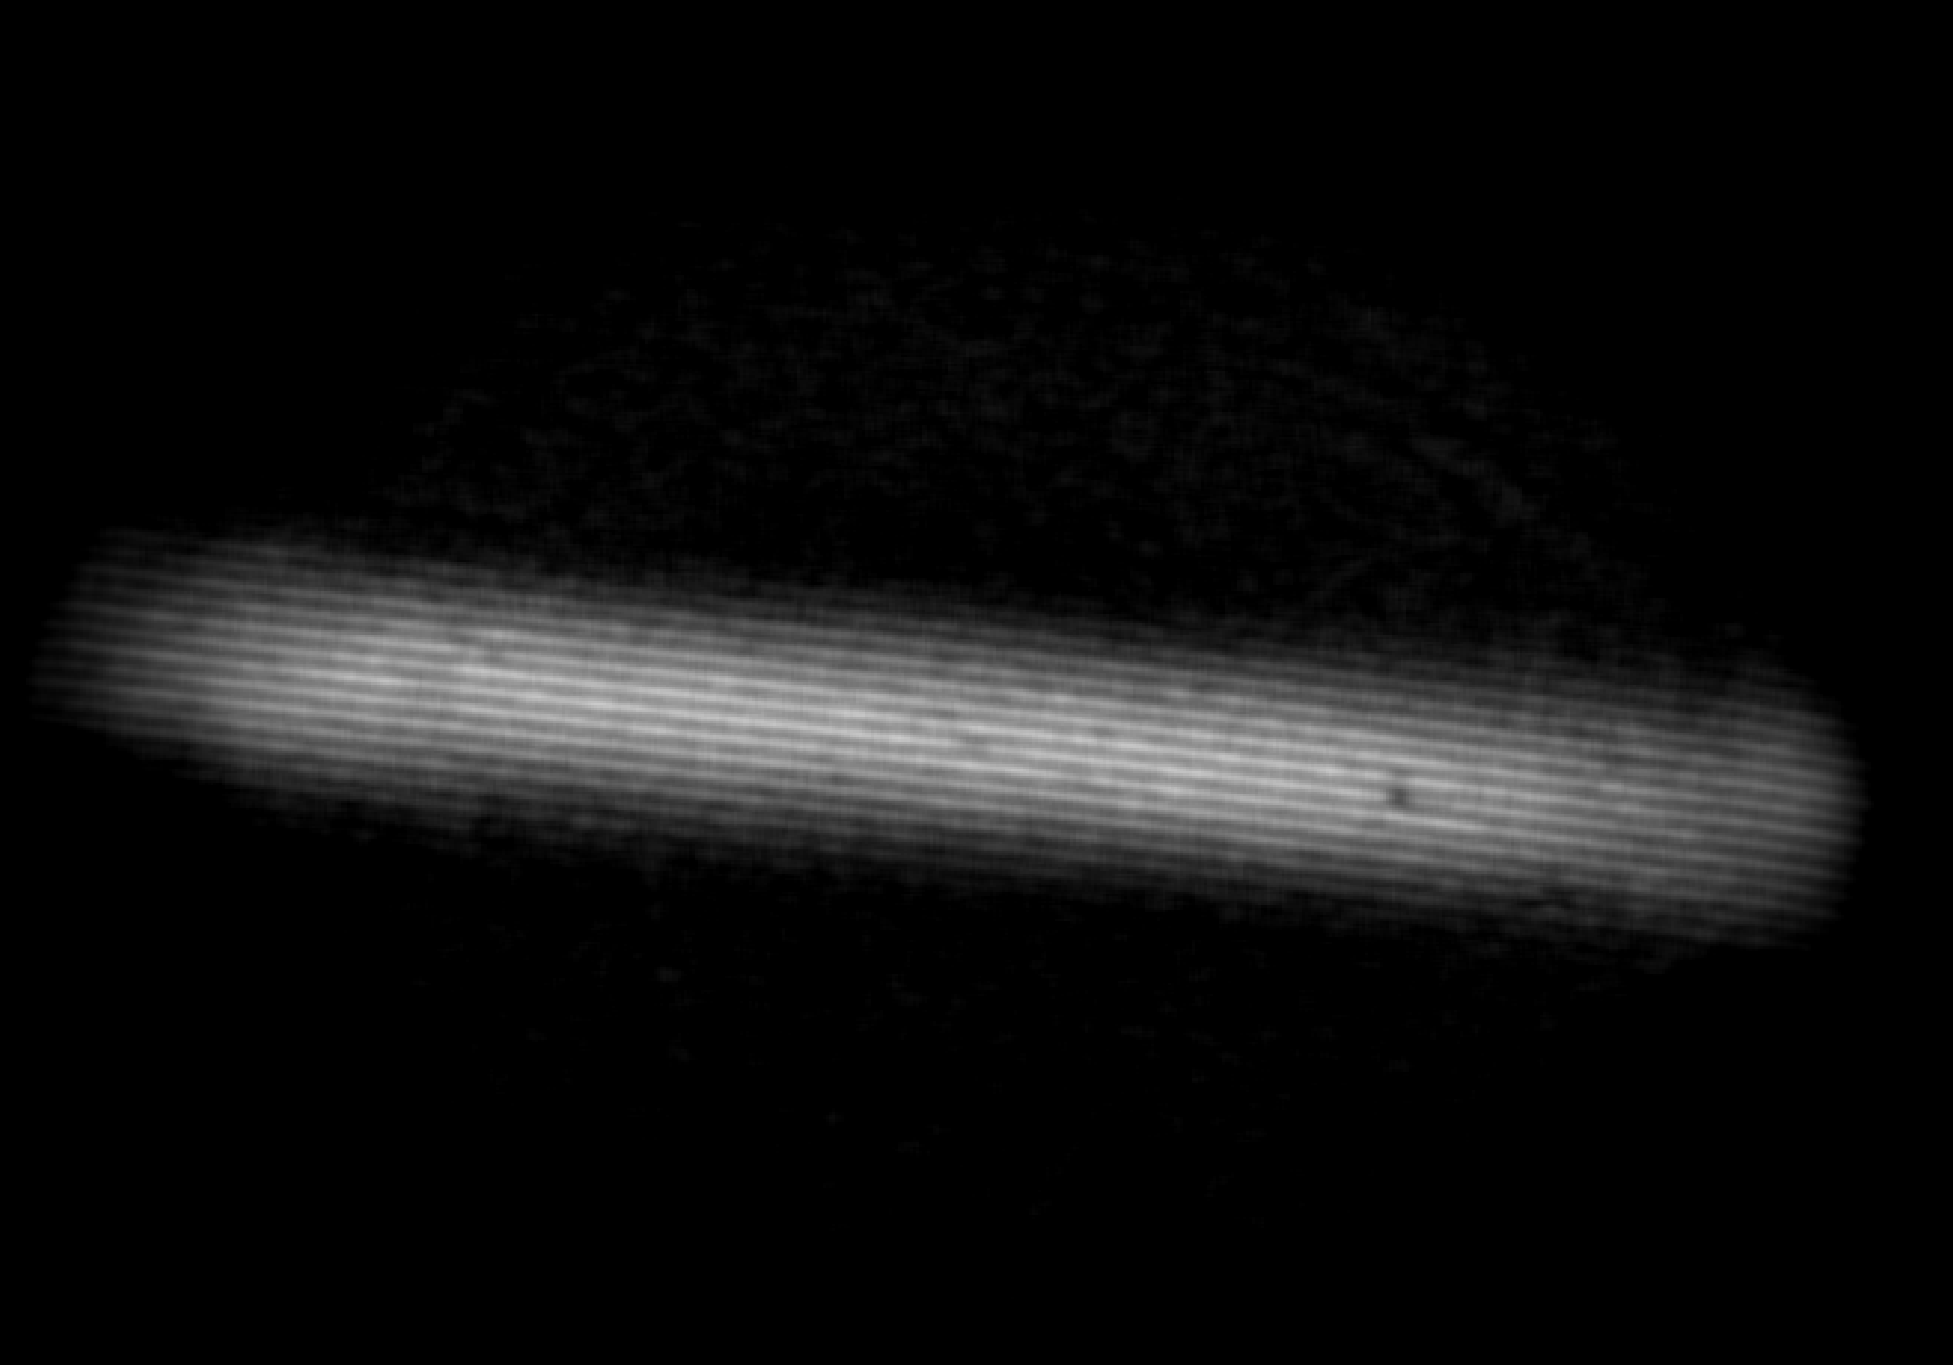
\includegraphics[width=0.49\linewidth]{img/chap2/Modulacion}}
	\caption[Patrón de interferencia con luz blanca]{Patrón de interferencia obtenido a partir de luz blanca, (a) corresponde a la interferencia directa, y (b) la modulación del patrón obtenido a partir del IPS.}
	\label{fig:modulacionfranjasluzblanca}
\end{figure}

Ahora bien, si se realiza un escaneo axial tomando imágenes de las franjas de interferencia a distintas profundidades, se obtienen desplazamientos del patrón proporcionales a la profundidad en la que se encuentren. Con estos datos se reconstruye el volumen, que en este caso contiene un único reflector. Luego de capturar el volumen, si se toma el escaneo de un punto de la imagen \enface se tiene el perfil de reflectividad contra profundidad en un punto de la muestra, esto corresponde a la definición de línea A. Para el pixel central de la Fig.~\ref{subfig:patroninterferencia}, la línea A correspondiente se muestra en la Fig.~\ref{subfig:lineaa}, para esta línea la reflectividad de la muestra corresponde a su modulación, la envolvente del reflector suavizada tomando los datos obtenidos por medio del IPS se presenta en la Fig.~\ref{subfig:lineaaenvelop}. 



%La línea A muestra cómo el patrón de interferencia de la fuente depende del espectro de la fuente y de la longitud de onda central que este posee. Como se conocen los desplazamientos realizados en profundidad, en este caso, de $FALTA$, se corrobora que el ancho a la mitad del máximo corresponde a $ $, con respecto al valor teórico calculado de $2.14\mu m$, con un error del $\%$.

%Para obtener la reflectividad de la muestra, es necesario tomar el patrón de interferencia que se muestra en la Fig.~ y obtener la modulación de las franjas. 
%El objetivo de los sistemas de OCT es poder obtener la modulación en el patrón de interferencia que se produce 

\begin{figure}[ht!]
	\centering
	\subfigure[Línea A correspondiente al pixel central.]{\label{subfig:lineaa}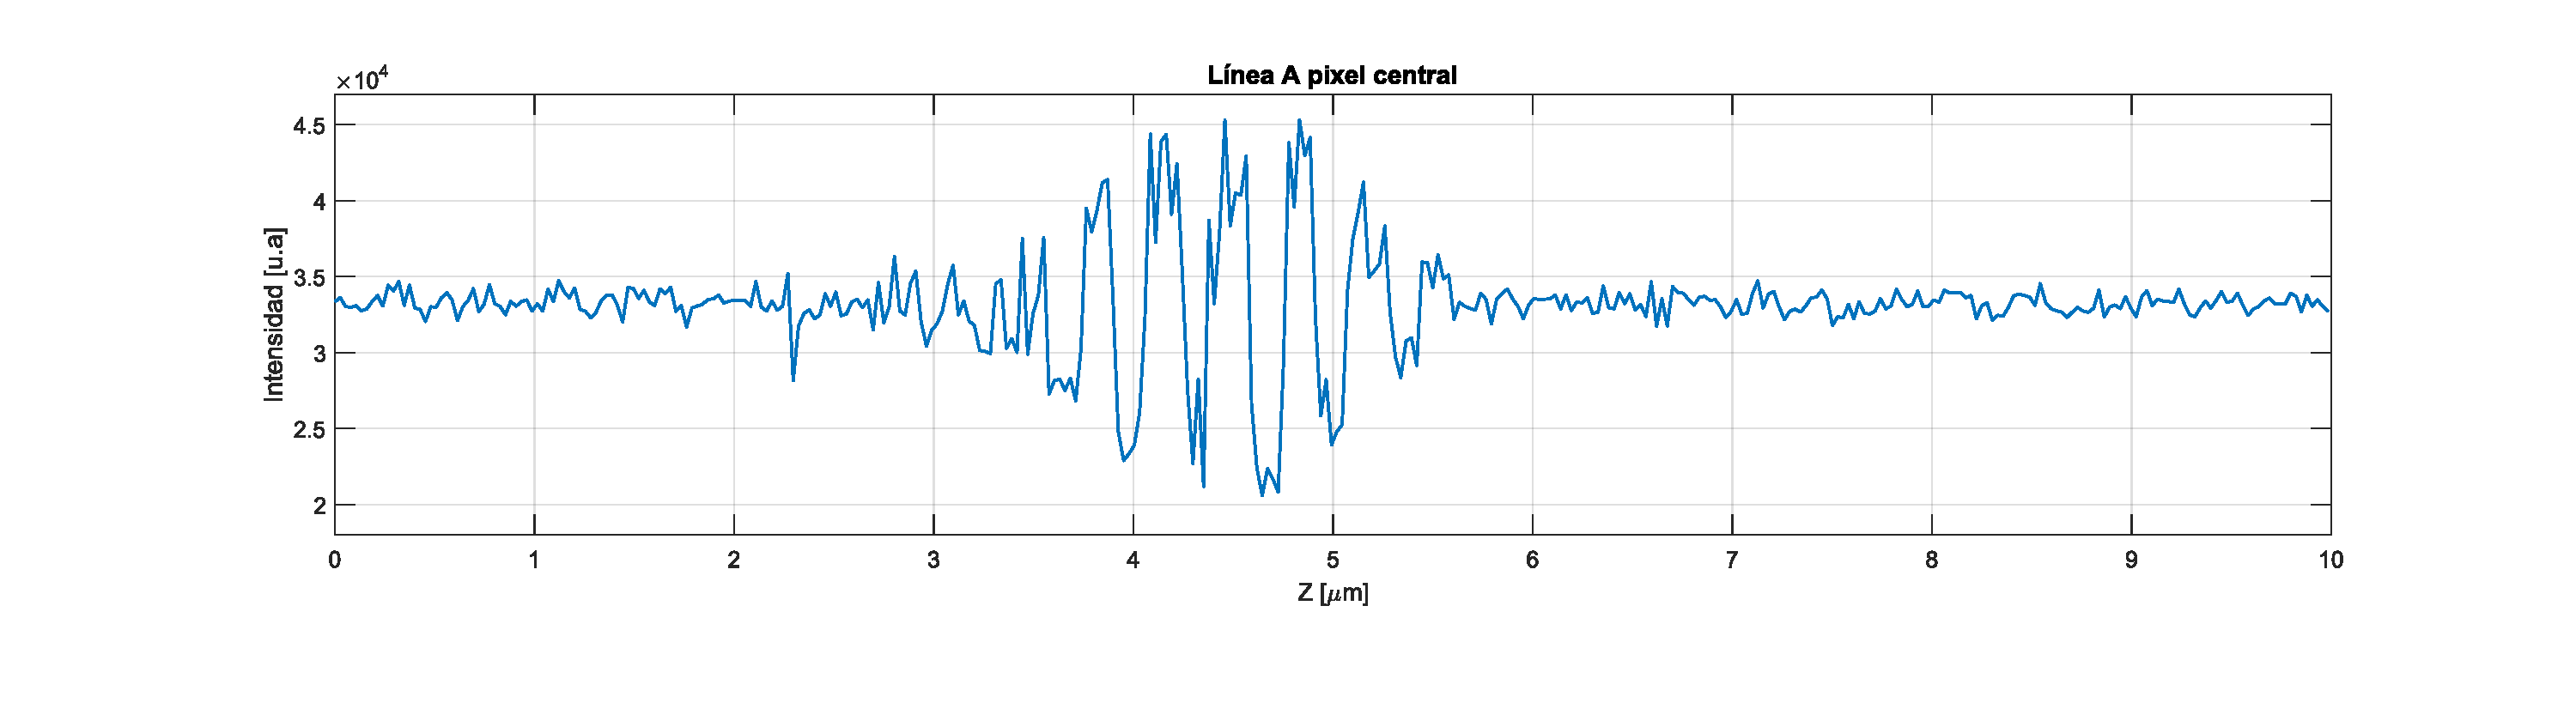
\includegraphics[width=1\linewidth]{img/chap2/LineaAPXCenter}}
	\subfigure[Envolvente de la línea A.]{\label{subfig:lineaaenvelop}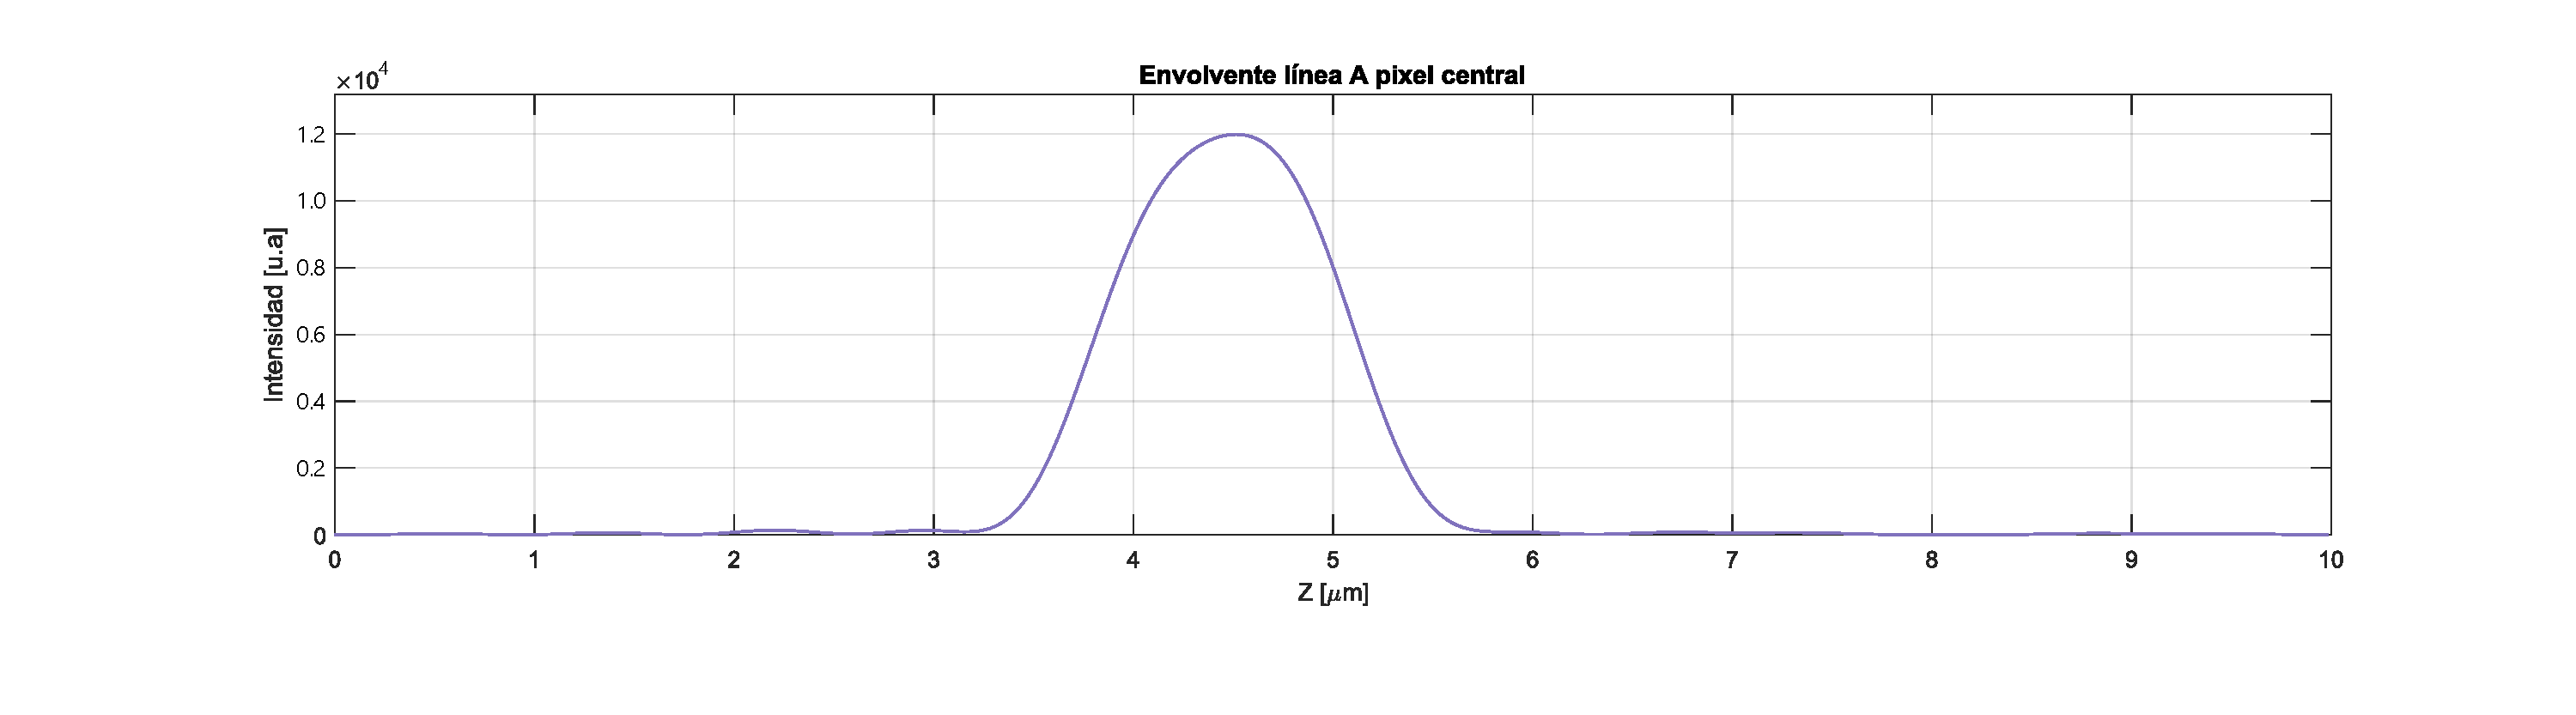
\includegraphics[width=1\linewidth]{img/chap2/LineaAPXCenterEnvelop}}
	\caption[Línea A medida experimentalmente]{Línea A correspondiente a un pixel, (a) patrón de interferencia registrado en profundidad, correspondiente a la definición de línea A, y (b) envolvente de la línea A, la altura de esta es la reflectividad de la muestra.}
	\label{fig:lineaa}
\end{figure}

%\subsubsection{Obtención de la modulación a partir del patrón de interferencia}
%
%
%
%Para obtener la modulación del patrón de franjas en un sistema de OCT, el proceso a seguir es similar al que se realiza en los algoritmos de reconstrucción de fase a partir de patrones de interferencia, por ejemplo, el algoritmo de cuatro pasos. En el algoritmo de cuatro pasos, cuatro patrones de interferencia con saltos de fase conocidos se registran $I_{1...4}$ y la fase se recupera a partir de la relación matemática
%
%\begin{equation}
%\phi = 
%\end{equation}
%
%Sin embargo, los sistemas interferométricos son altamente sensible a las vibraciones, ya que registran desplazamientos del orden de la longitud de onda. Es por ello, que para obtener la modulación, se empleó el algoritmo conocido como algoritmo de salto de fase iterativo (IPS: \textit{iterative phase shifting}). De manera similar al algoritmo de cuatro pasos, el IPS busca encontrar la fase $\phi$, con la diferencia de buscar también los saltos de fase $\delta \phi$ entre los interferogramas que se ingresan al algoritmo de manera iterativa, por lo tanto es menos sensible ante las oscilaciones del sistema. El proceso de encontrar la fase y los saltos de fase, requiere también la obtención de la modulación del patrón de interferencia, esta es la que se desea obtener en el caso de OCT.
%
%A partir de la captura de cuatro interferogramas con diferentes (y desconocidos) saltos de fase por profundidad, la modulación del patrón de interferencia mostrado en la Fig.~ puede obtenerse, esto se muestra en la Fig.~, así mismos, la modulación o envolvente de la línea A central, corresponde a la mostrada en la Fig.~.
%
Como conclusión, la obtención de la reflectividad de la muestra en cada profundidad medidas con el IPS requiere que se capturen al menos cuatro imágenes con diferentes saltos de fase \cite{Wang2004}, la ventaja fundamental de este algoritmo es que no requiere saltos de fase conocidos y por tanto es menos susceptible a vibraciones en el sistema óptico. Al ser un algoritmo iterativo, el resultado que éste brinda puede mejorarse si se incluye una cantidad mayor de interferogramas en el algoritmo, por lo tanto, cuando haya una alta absorción por parte de la muestra y un bajo contraste del patrón de interferencia, se puede incrementar la cantidad de imágenes capturadas, ya que esto ayuda a diferencia la región de la imagen con interferencia de aquellas regiones en donde se encuentra el ruido.

\subsubsection{Parámetros del montaje}

Los parámetros más importantes que determinan el desempeño del montaje y la forma en la que se midieron se relacionan a continuación:

\begin{itemize}
\item \textbf{Resolución lateral:} La resolución lateral está determinada por la capacidad para desplazarse en los ejes $x$ y $y$, en el caso de OCT de campo completo, esta resolución la indica el tamaño del pixel del detector que es $3.69\mu m$. 

\item \textbf{Resolución axial:} Determinada por la longitud de coherencia de la fuente, la resolución axial obtenida fue de $2.14\mu m$.

%\item \textbf{Profundidad de foco:} La profundidad de foco determina la región en la cual el haz enfocado no se desvía más de $\sqrt{2}w_0$, donde $w_0$ es el ancho del haz enfocado. Calculado con la Eq.~\ref{eq:depth_of_focus}, es de

%\begin{equation}
%b = \frac{4(3.16\times 10^{-6}m)}{\pi}\left( \frac{10^{-3}m}{5.08\times 10^{-3}m}\right) = 7.92\mu m
%\end{equation}

\item \textbf{Desplazamiento axial mínimo y máximo:} El paso mínimo que es posible dar en el sistema corresponde al menor desplazamiento que puede realizar el piezoeléctrico, en este caso $26.66nm$. Sin embargo, por la resolución axial, el desplazamiento se mantuvo en $1\mu m$. La distancia máxima que se puede recorrer es una combinación del desplazamiento máximo del piezoeléctrico $20\mu m$ y el desplazamiento manual que puede hacerse con el tornillo micrométrico, cuya resolución es de $10\mu m$ y un recorrido total de $1.5cm$. Para profundidades mayores a $20\mu m$, es necesario una combinación entre recorrido manual con el tornillo micrométrico y el piezoeléctrico.

\item \textbf{Sensibilidad:} La sensibilidad del sistema se midió ubicando filtros de densidad neutra de diferentes densidades en el haz objeto, instalando detrás de éste un espejo, de forma que la luz viaja dos veces por el filtro. La máxima densidad para la cual fue posible obtener interferencia fue de $1.8$, es decir, $10^{-3.6}\approx 0.25\times 10^{-3}$ veces la intensidad de entrada ó $-36dB$, considerando que la doble atenuación que sufre la luz en el filtro.


\end{itemize}

%En la Tabla~ se muestran los parámetros finales del montaje implementado

\subsection{Resultados obtenidos}
\label{sec:resultados}
\subsubsection{Topografía de la moneda}

La moneda con la cual se realizó la reconstrucción de topografía se presenta en la Fig.~\ref{fig:Moneda_Directa_img}, la zona de la imagen que se encuentra aumentada y señalada por la línea roja punteada, fue la región en la que se tomaron las imágenes. Mediante el procedimiento de recuperación de la modulación empleando ocho imágenes con el IPS a partir del patrón de franjas, se realizó un escaneo axial de la moneda con desplazamientos en la dirección $Z$ de $1\mu m$. La modulación obtenida a partir de los patrones de interferencia capturados a diferentes profundidades se muestra en la Fig.~\ref{fig:Enface_Sequence}, las regiones en donde se encuentra interferencia corresponden a las profundidades de la moneda que diferencia en altura es menor a la longitud de coherencia. 

\begin{figure}[!h]
	\centering
	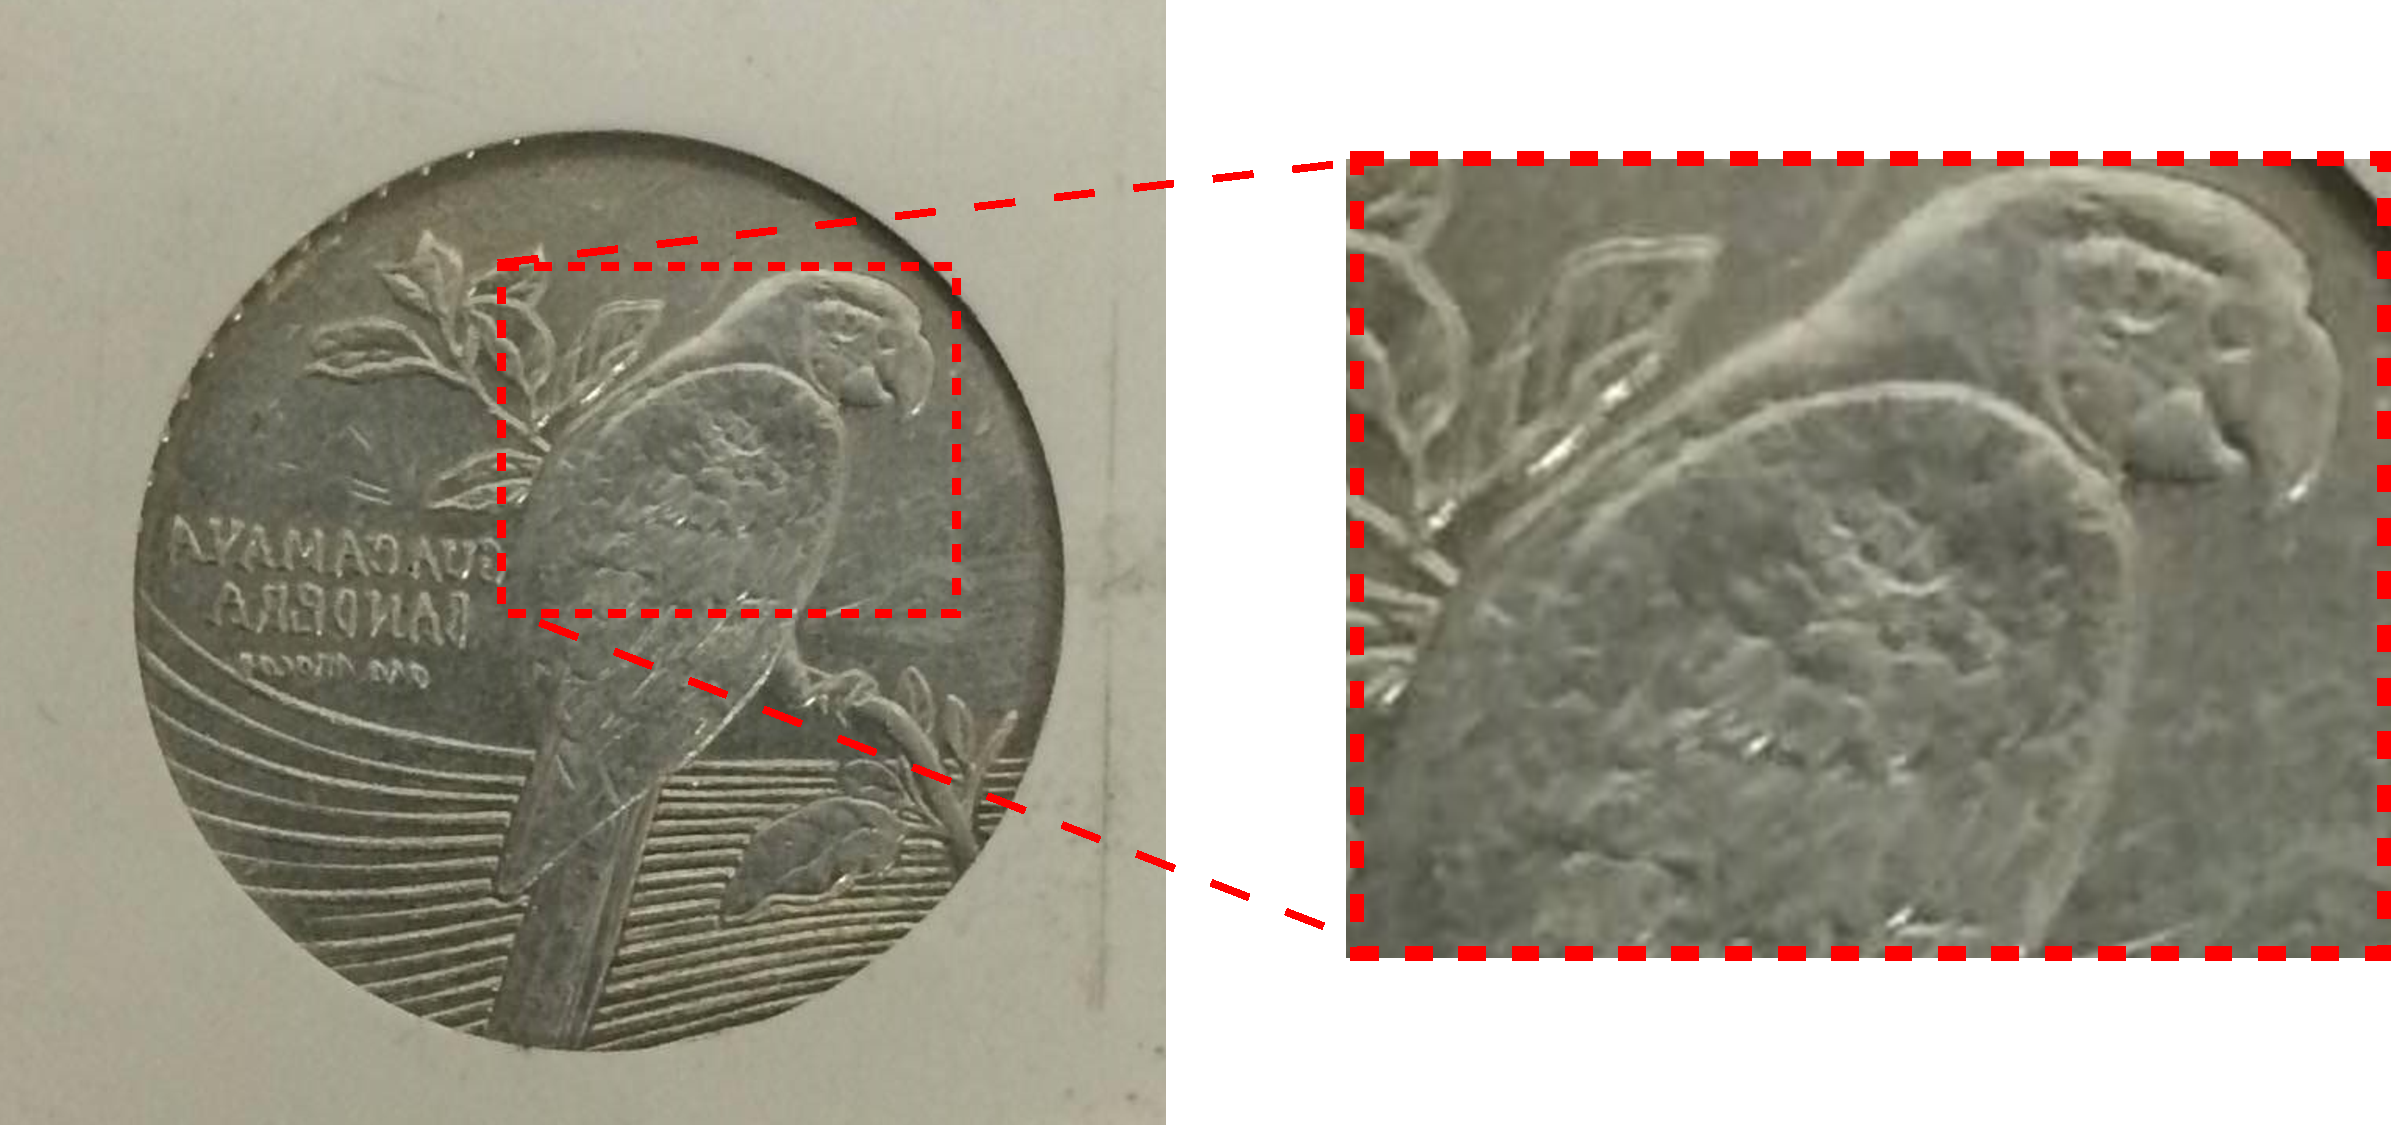
\includegraphics[width=0.6\linewidth]{img/chap2/Moneda_Directa_img}
	\caption[Moneda empleada en las mediciones.]{Moneda empleada para las mediciones con OCT, el área aumentada corresponde a la sección de la imagen capturada para la reconstrucción.}
	\label{fig:Moneda_Directa_img}
\end{figure}

Las imágenes que se presentan en la Fig.~\ref{fig:Enface_Sequence}, fueron capturadas de izquierda a derecha y de arriba hacia abajo, con una separación de $20\mu m$; en ellas se evidencia cómo la interferencia realiza un escaneo secuencial en la moneda por las diferentes profundidades del relieve que posee, comenzando por la zona inferior, en donde las características del grabado hacen que esta región del relieve se sitúe a una altura mayor, apareciendo primero en la secuencia de interferogramas. A continuación, se escanea la zona central de la moneda, hasta la parte superior, en donde se tiene la región plana y homogénea que posee la moneda. La progresión que sigue la modulación en las imágenes también indica que el haz referencia y el haz objeto no están completamente alineados, ya que la interferencia en las regiones planas de la imagen no ocurren de manera simultánea en una profundidad específica, sino que se encuentra distribuida a lo largo de diferentes profundidades.
\begin{figure}[!h]
	\centering
	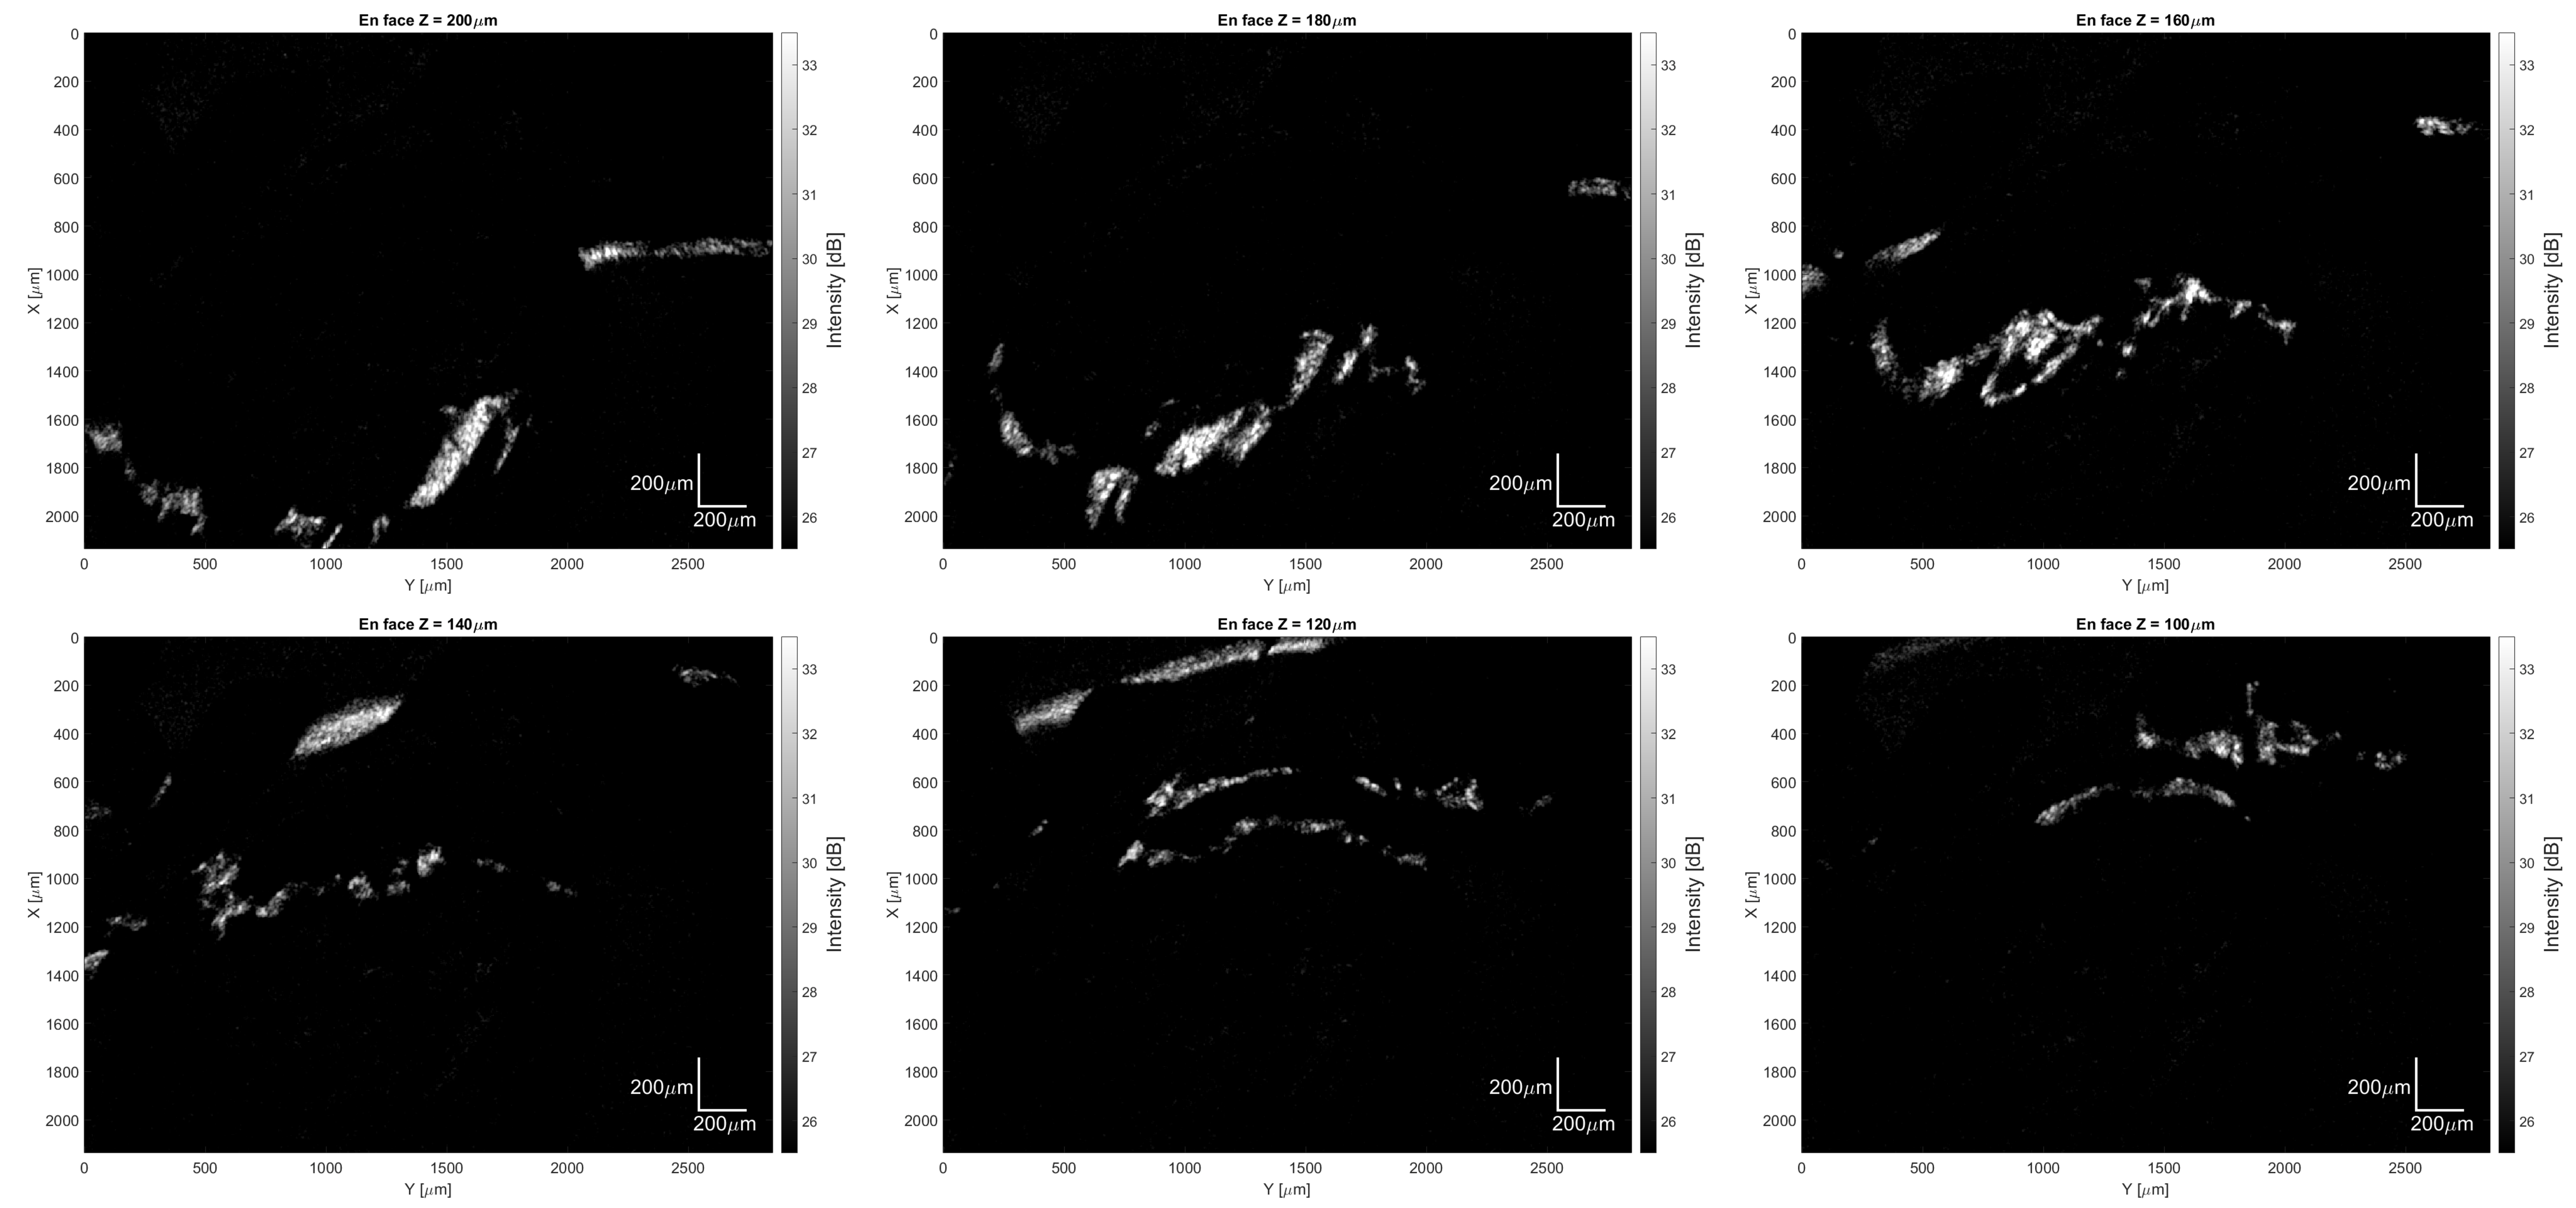
\includegraphics[width=1.0\linewidth]{img/chap2/Enface_Sequence}
	\caption[Secuencia de imágenes capturadas por la cámara.]{Secuencia de imágenes capturadas para la reconstrucción de la topografía de la moneda, la profundidad de cada imagen tiene una diferencia de $20\mu m$.}
	\label{fig:Enface_Sequence}
\end{figure}
\noindent Luego de escanear un total de $300\mu m$ en profundidad, se realizó la suma de las modulaciones obtenidas a lo largo de las diferentes posiciones axiales, ésta imagen es equivalente a la proyección bidimensional que una cámara tomaría de la moneda. El resultado de la proyección obtenida con OCT se presenta en la Fig.~\ref{subfig:monedareconstrucoct}, mientras que en la Fig.~\ref{subfig:monedaimagendirecta} se encuentra la imagen de la moneda capturada directamente por la cámara.

\begin{figure}[h!]
	\centering
	\subfigure[Imagen reconstruida a través de OCT.]{\label{subfig:monedareconstrucoct}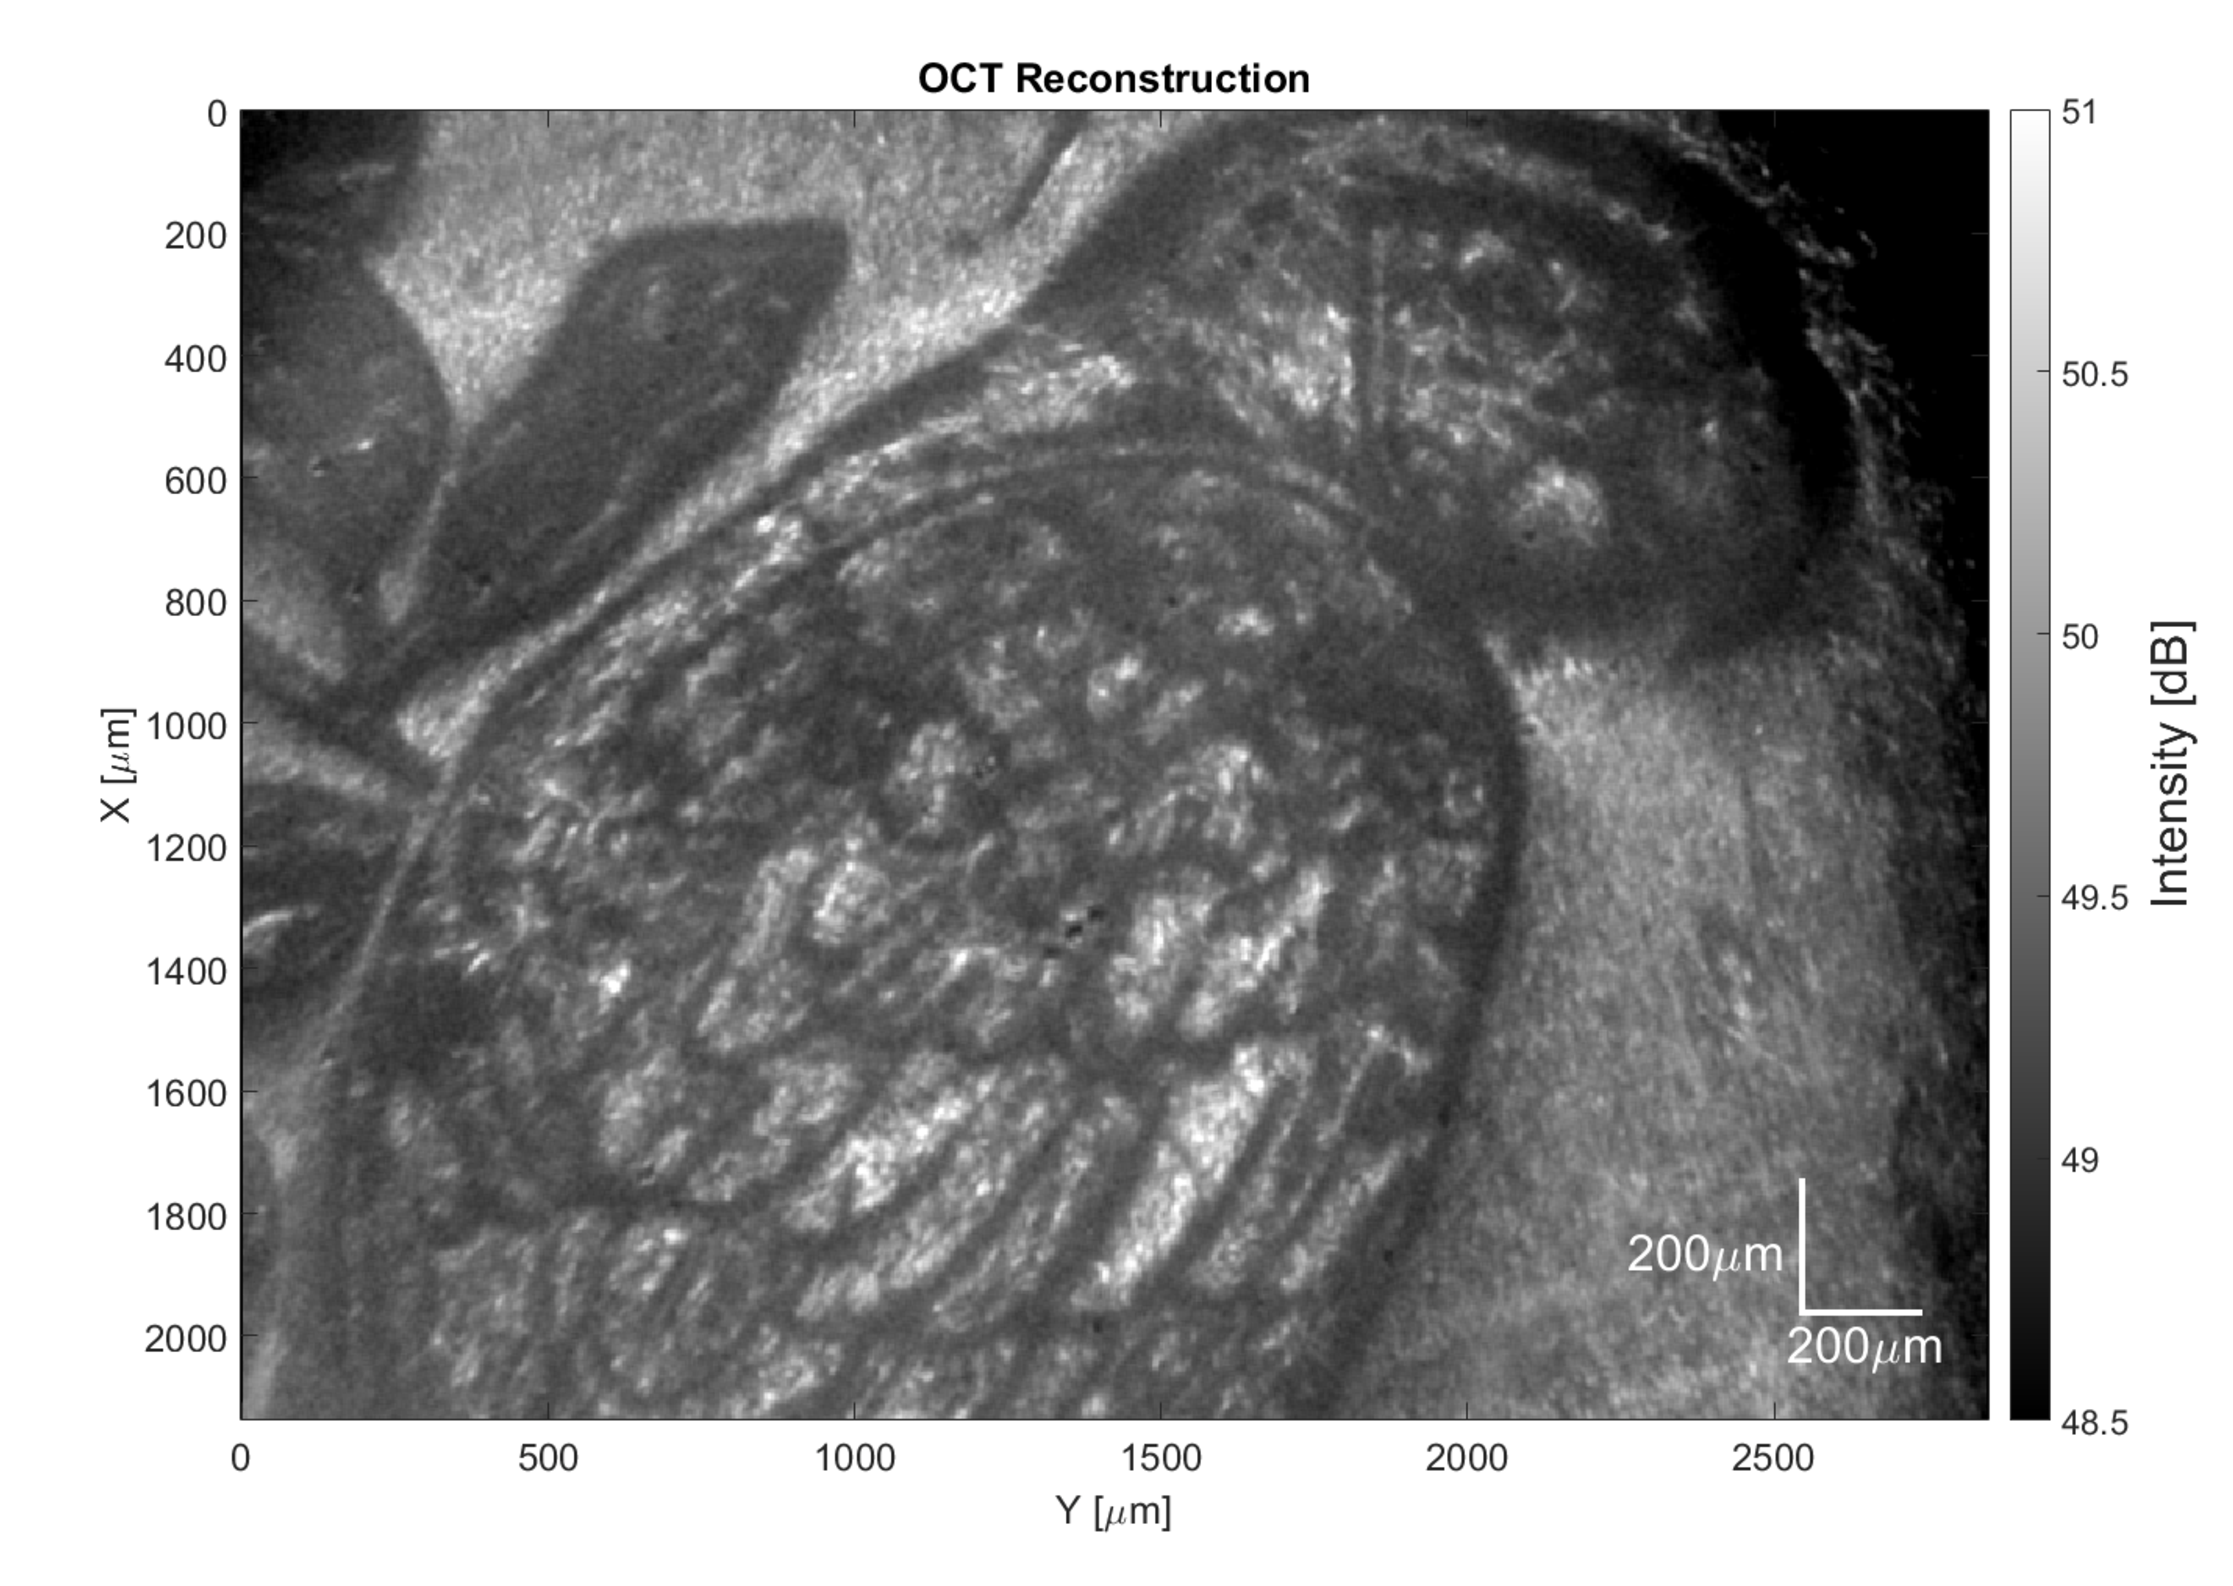
\includegraphics[width=0.49\linewidth]{img/chap2/OCT_En_face_Projection}}
	\subfigure[Imagen directa capturada por la cámara.]{\label{subfig:monedaimagendirecta}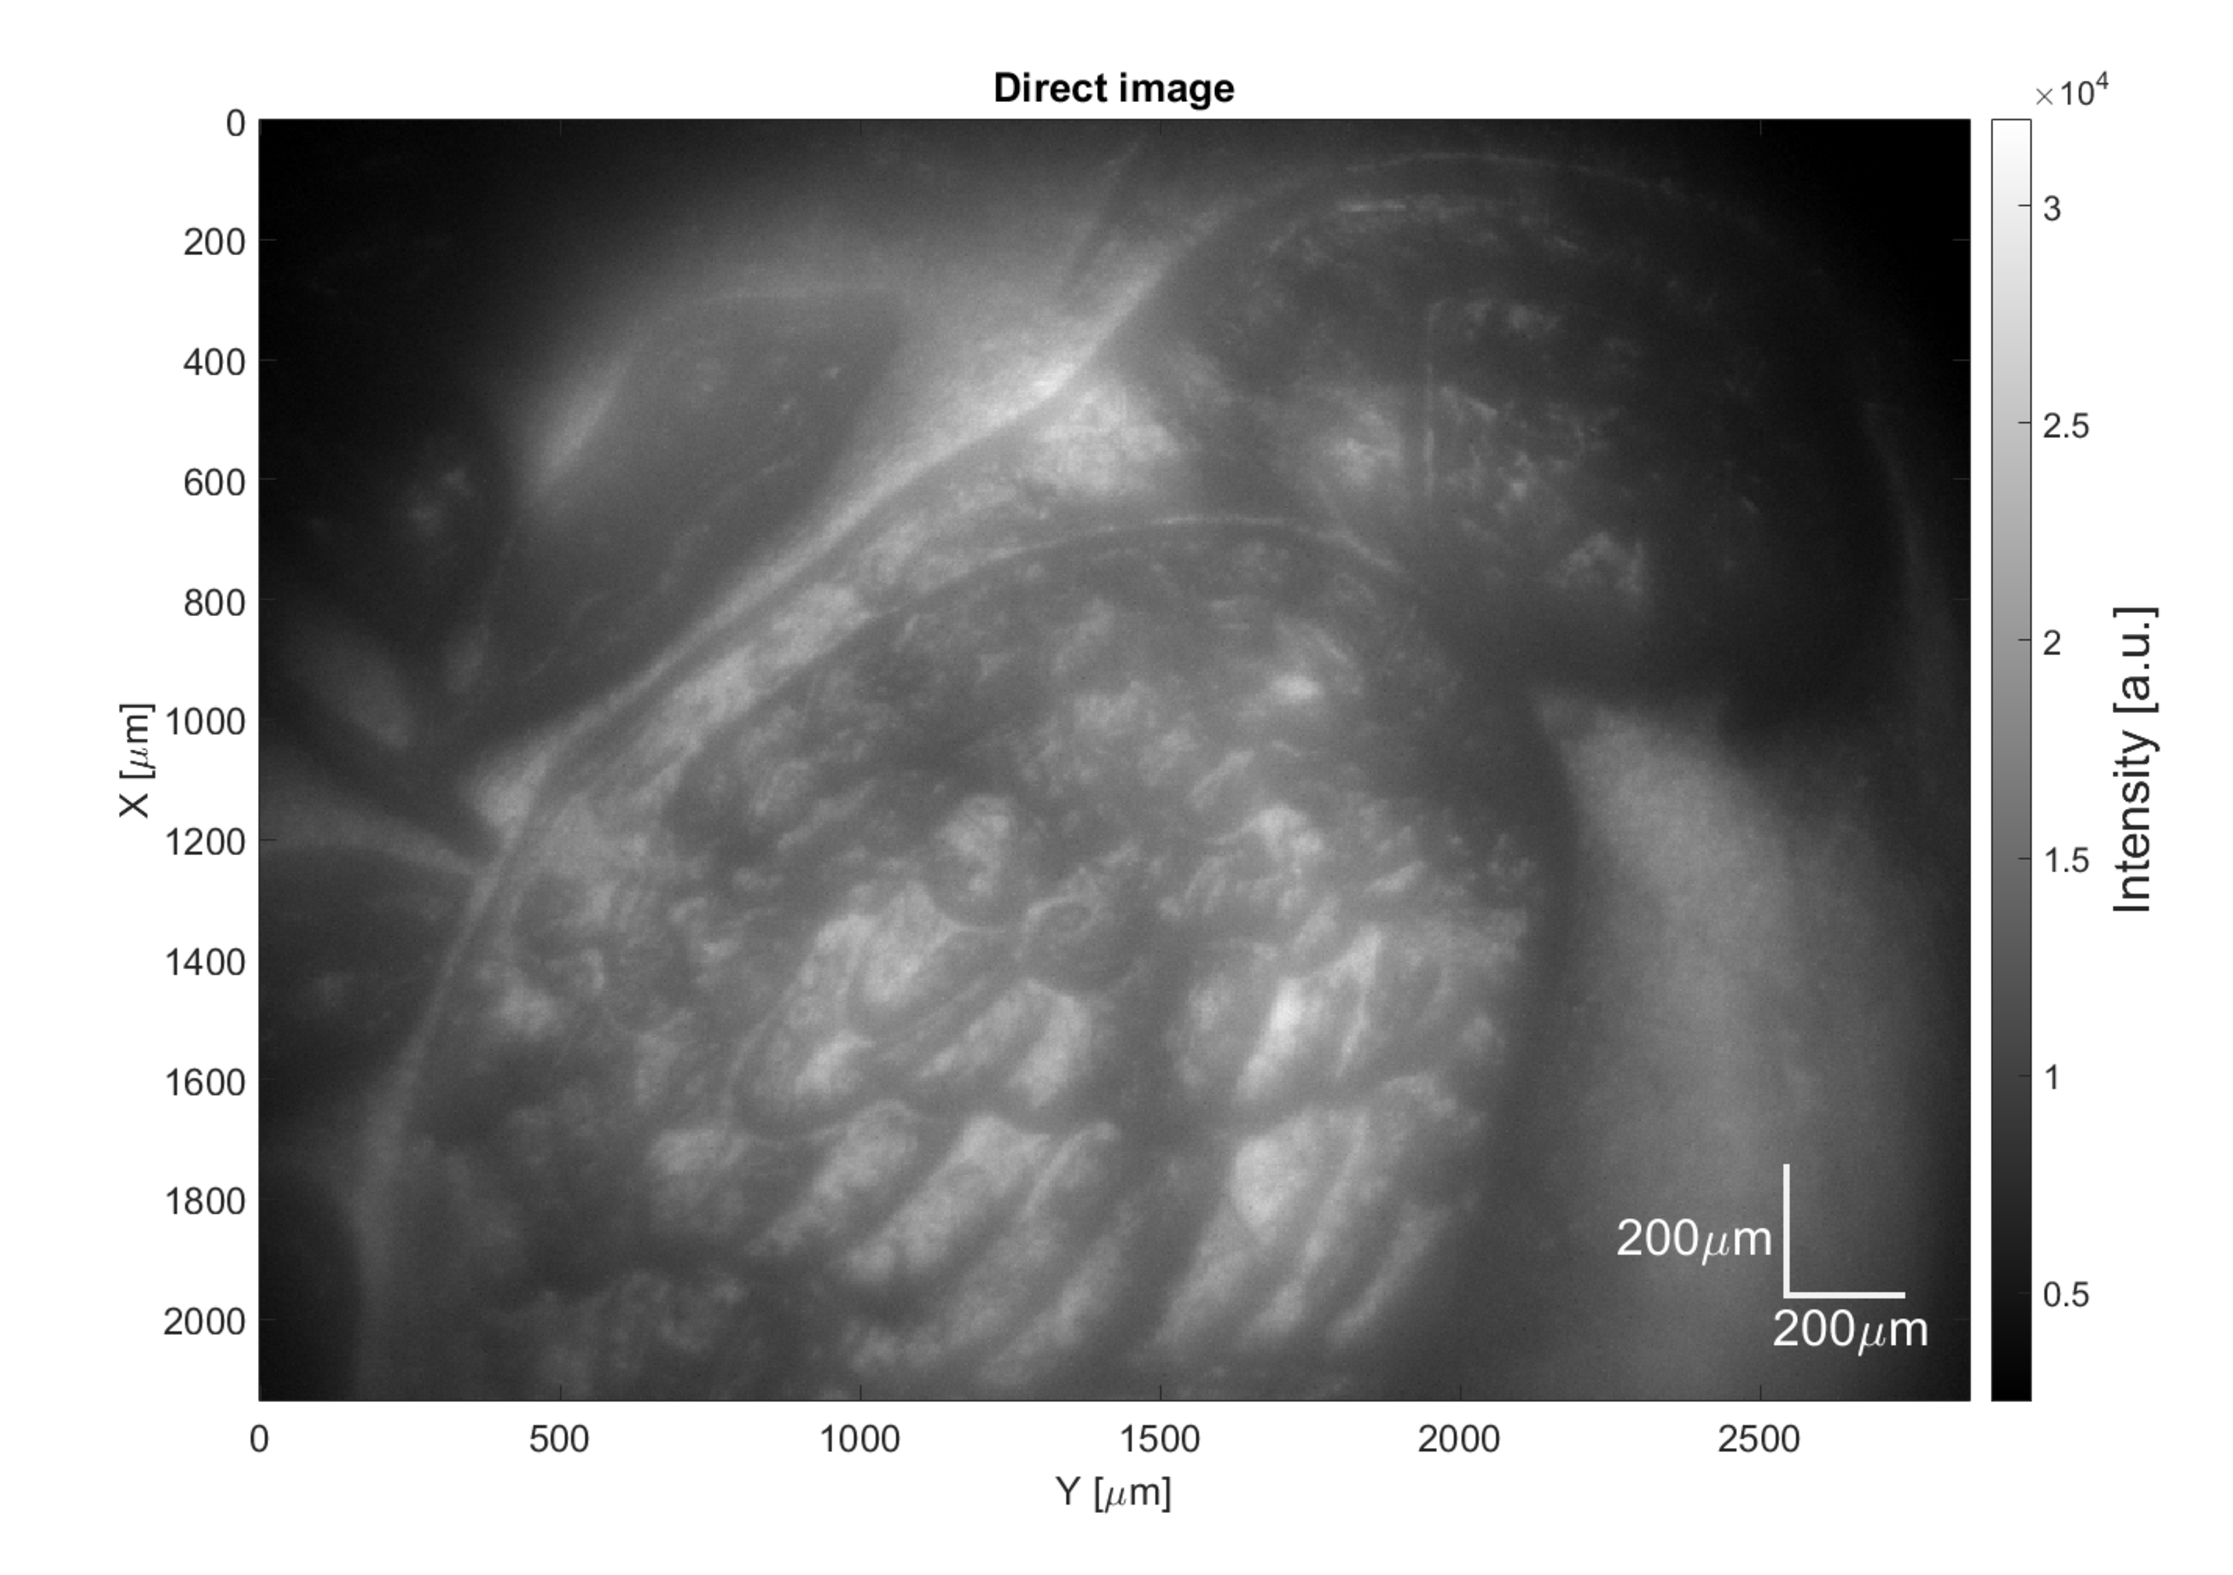
\includegraphics[width=0.49\linewidth]{img/chap2/Direct_image_Moneda_Final}}
	\caption[Comparación de imágenes capturadas con la moneda]{Comparación de la imagen capturada directamente por la cámara con la reconstruida mediante la proyección en dirección $Z$ con OCT.}
	\label{fig:comparacionimgdirecta}
\end{figure}

Como el desplazamiento axial y el tamaño del pixel son conocidos, se pueden tomar cortes de las secciones transversales de moneda, los cuales muestran el relieve que posee a lo largo de uno de los ejes. Tomando dos secciones transversales en los ejes $ZX$ y $ZY$, ubicados en $Y = 1.06mm$ y $X = 1.71mm$ respectivamente, como se indica en líneas blancas punteadas en la Fig.~\ref{fig:OCT_Reconstruction_Moneda}, se pueden analizar algunos puntos de interés ($A-H$) en la moneda. Los puntos $A$, $B$, $C$ y $D$ se encuentran localizados a lo largo del eje $X$ y señalan en su respectivo orden: ($A$) sección plana de la moneda, ($B$) transición entre el inicio del relieve y la sección plana, ($C$) zona con alta dispersión, y ($D$) región con relieve. Los puntos $E$, $F$, $G$ y $H$ están sobre el eje $Y$, y en orden corresponden a: ($E$) primera zona plana de la moneda, ($F$) zona con alta intensidad en el relieve, ($D$) transición entre el relieve y la segunda zona plana, y ($E$) región plana. Las secciones transversales señaladas anteriormente se muestran en la Fig.~\ref{fig:monedabscan}.


\begin{figure}[!ht]
	\centering
	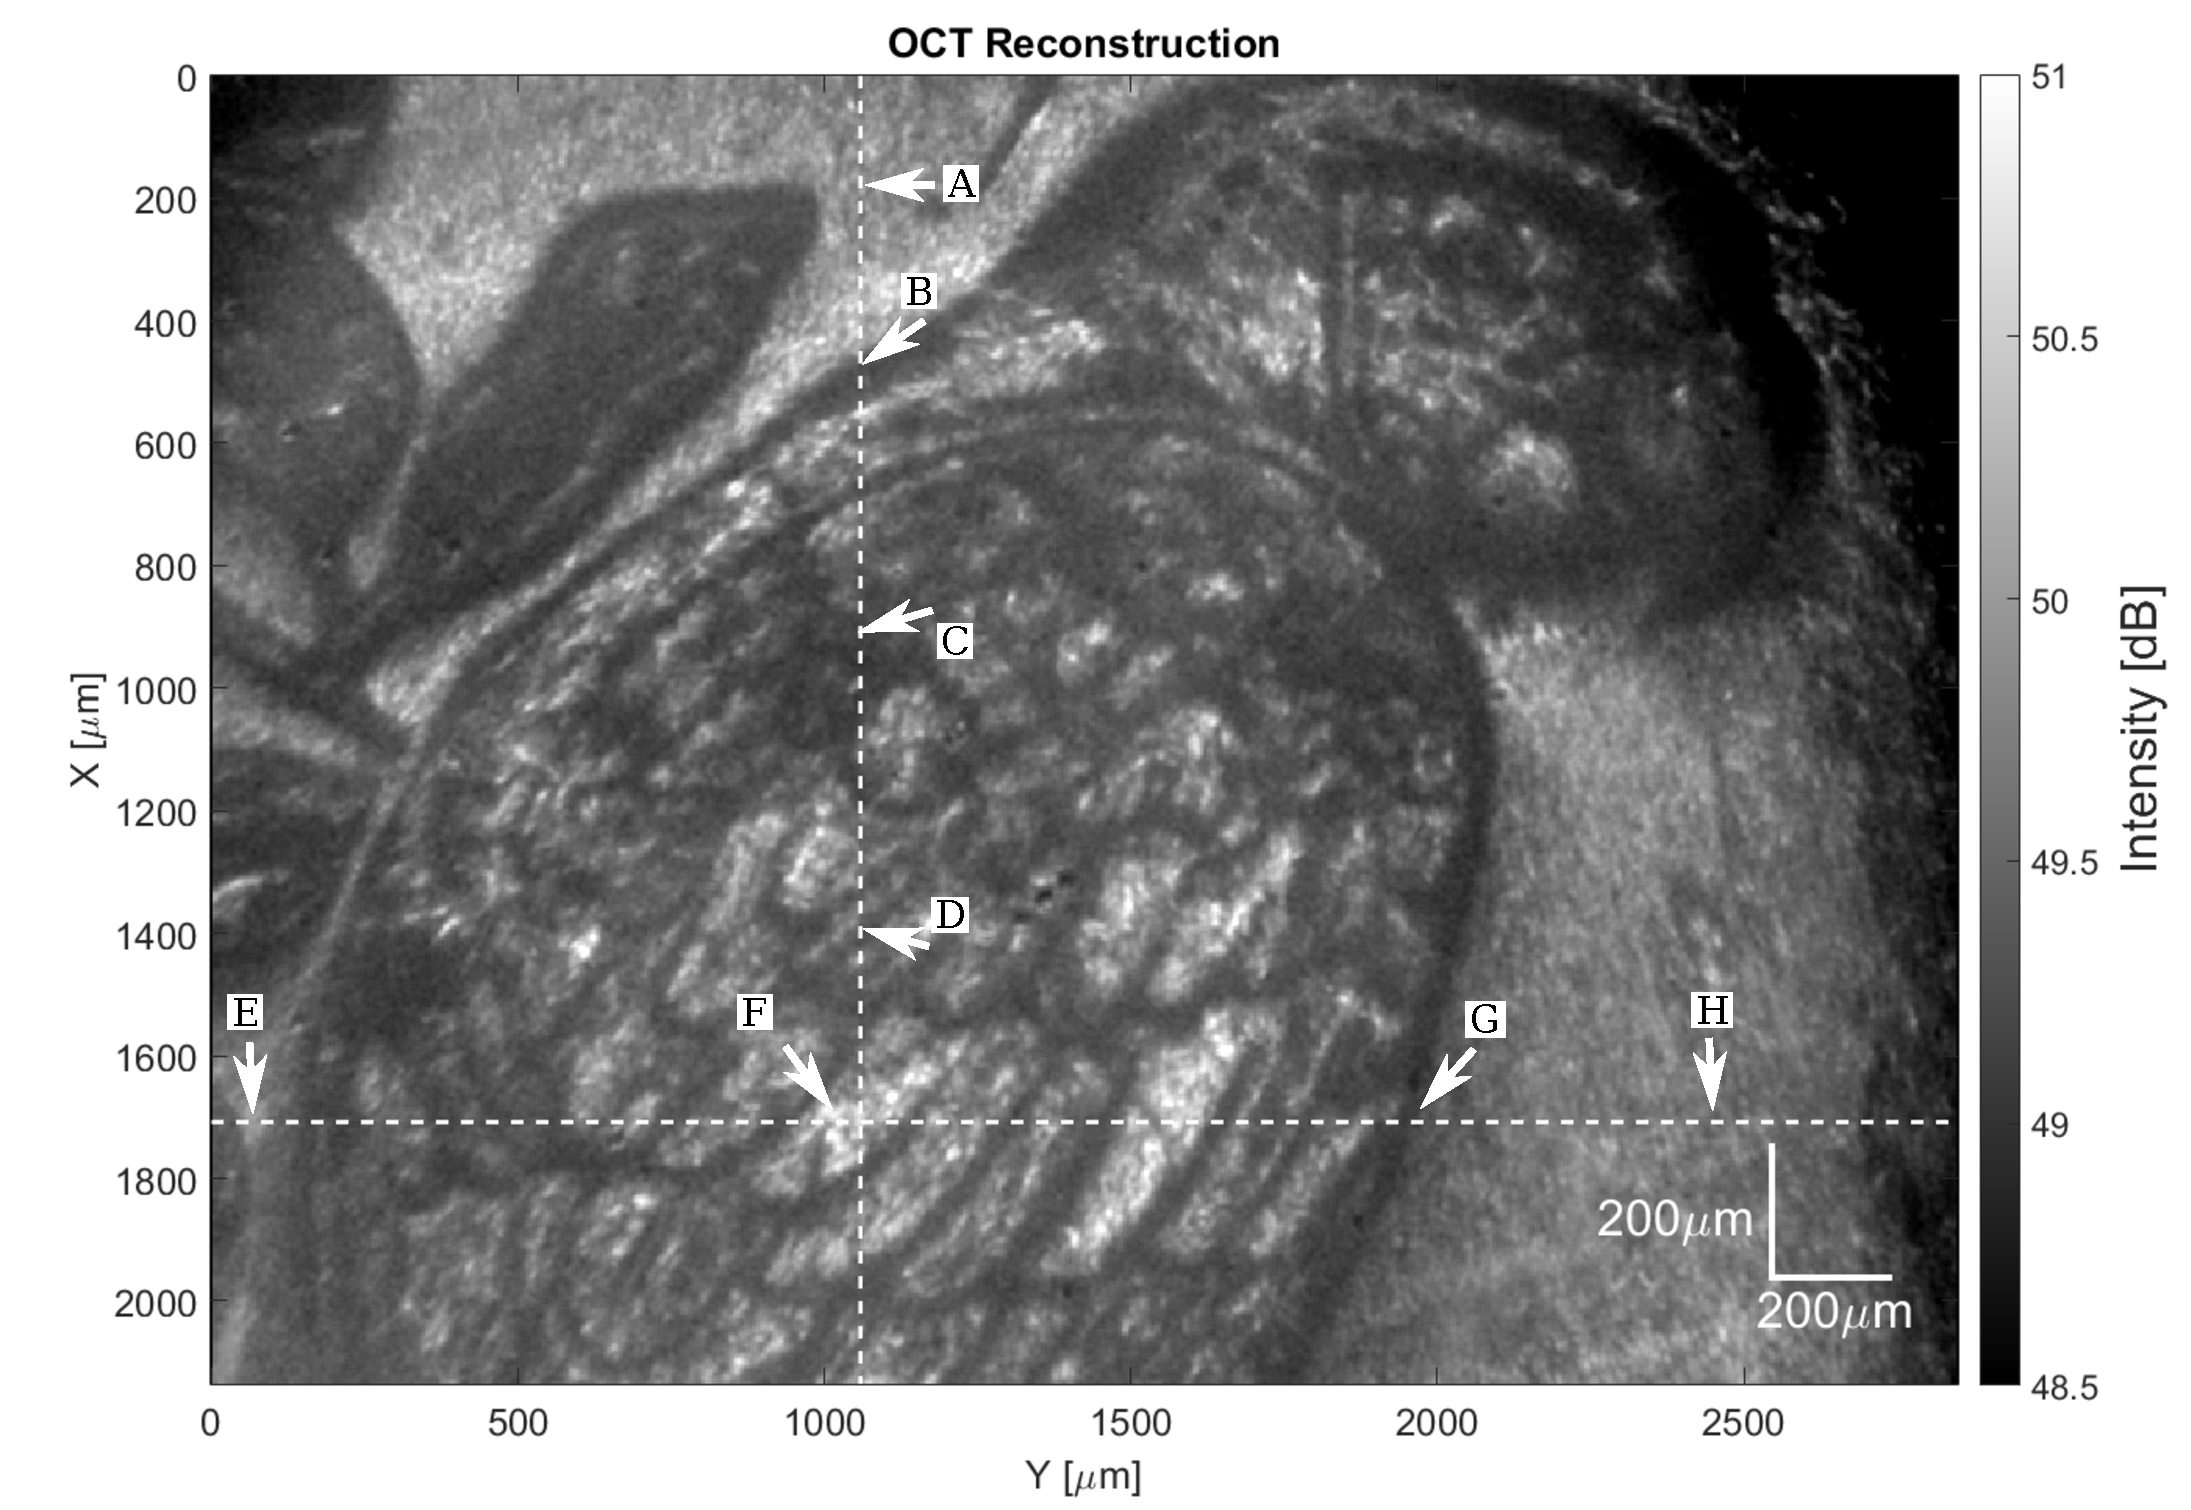
\includegraphics[width=0.7\linewidth]{img/chap2/OCT_Reconstruction_Moneda}
	\caption[Imagen de la moneda obtenida mediante la suma de todas las profundidades.]{Imagen obtenida con OCT a través de la suma de las diferentes imágenes en profundidad capturadas, esta corresponde a una captura similar a las realizadas por las cámaras. Los puntos indicados representan lugares de interés que se discuten en el texto.}
	\label{fig:OCT_Reconstruction_Moneda}
\end{figure}
La Fig.~\ref{subfig:Bscan_Moneda}, correspondiente a la sección transversal en el plano $ZX$, se le conoce como escaneo tipo B y está ubicado a una distancia $Y = 1.06mm$. En este caso, a lo largo del eje $X$ se observa unicamente la presencia de un reflector en todas las profundidades $Z$, lo que es de esperar debido a que la moneda solamente refleja luz sobre la superficie antes de absorber o reflejar la luz que llega hasta ella. Como se conoce la distancia axial escaneada y el tamaño de cada paso, se concluye que el relieve de la moneda presenta tiene una altura máxima de $\approx 50\mu m$. En la sección transversal se distinguen los puntos $A-D$ sobre el eje $X$, indicados anteriormente. El punto $A$ muestra una región plana a lo largo de $X\approx 0-500\mu m$, seguida por el punto $B$ como una zona oscura de transición a una altura mayor. $C$ aparece como una pequeña región oscura, que indica una alta dispersión de la luz en la moneda. Por último, el punto $D$ muestra una zona con fluctuaciones para $X\approx 1350-1450\mu m$. La Fig.~\ref{subfig:ZYPlane_moneda}, que es un corte en el plano $ZY$ presenta una variación en profundidad menor, pero como se mencionó, esto está relacionado con la inclinación del haz objeto con respecto al de referencia. Los puntos $E$ y $H$ muestran dos zonas donde la profundidad es constante a lo largo de $Y\approx 50-150\mu m$ y $Y\approx 2000-2800\mu m$, representando regiones planas. Alrededor del punto $F$ se encuentra una pequeña zona homogénea pero discontinua por la transición entre las diferentes alturas del relieve. El punto $G$ es la transición de la zona con relieve hasta el área plana, y es por ello que aparece como un punto opaco. Una mayor intensidad en la imagen, representa que la luz ha sido reflejada por la moneda en la dirección del detector, mientras que una baja intensidad, muestra que la moneda refleja la luz en direcciones aleatorias o la absorbe. 
\begin{figure}[h!]
	\centering
	\subfigure[Plano $ZX$ o escaneo B obtenido con la topografía de la moneda.]{\label{subfig:Bscan_Moneda}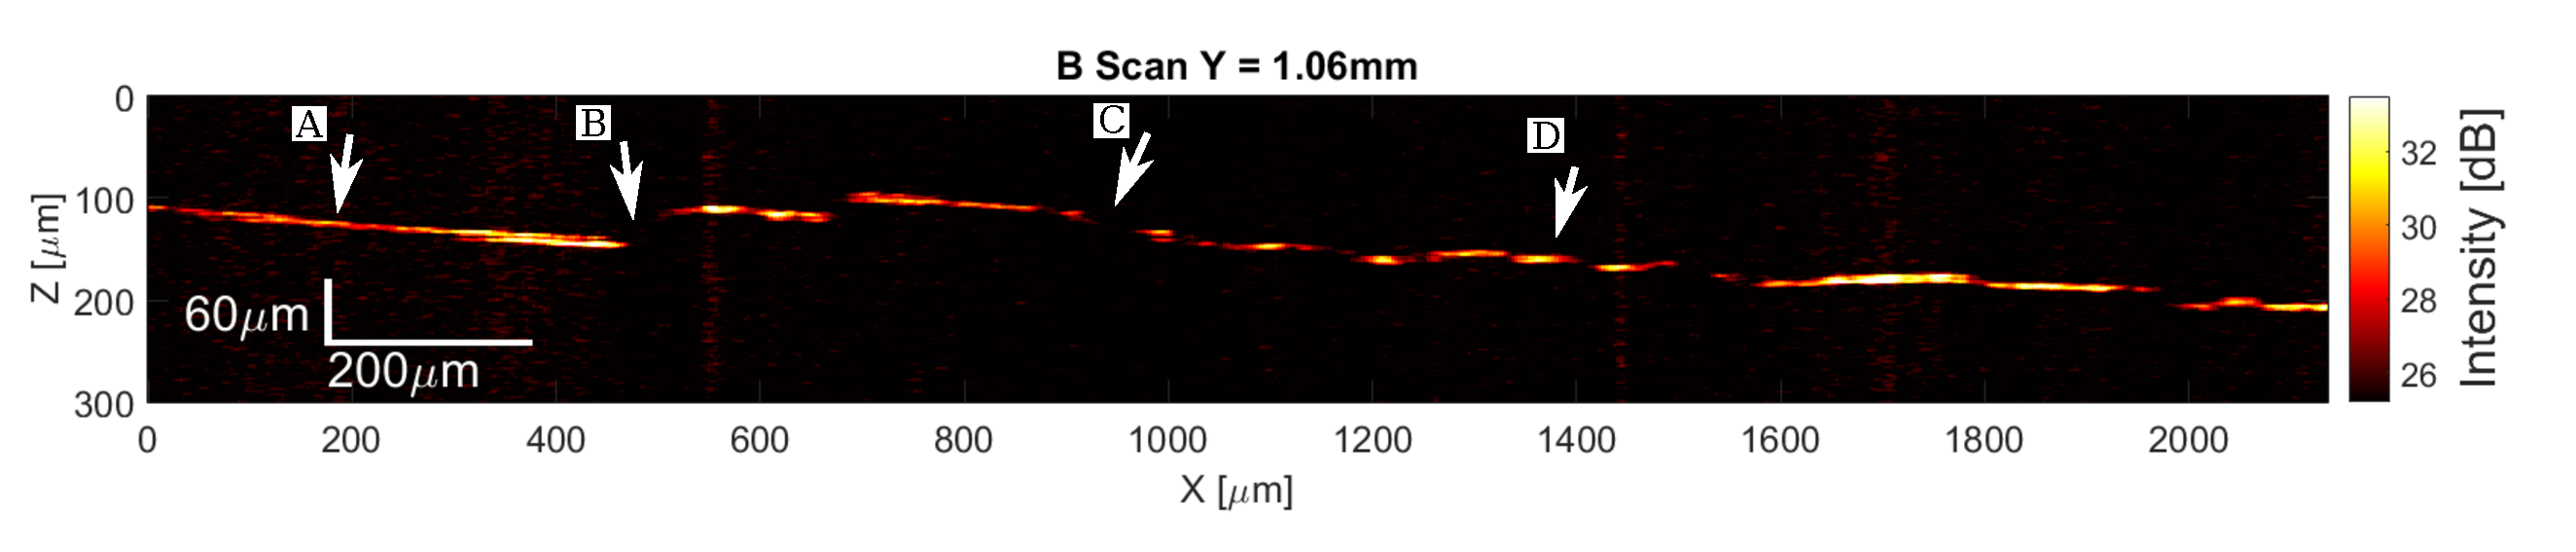
\includegraphics[width=0.97\linewidth]{img/chap2/Bscan_Moneda}}
	\subfigure[Plano $ZY$ obtenido con la topografía de la moneda.]{\label{subfig:ZYPlane_moneda}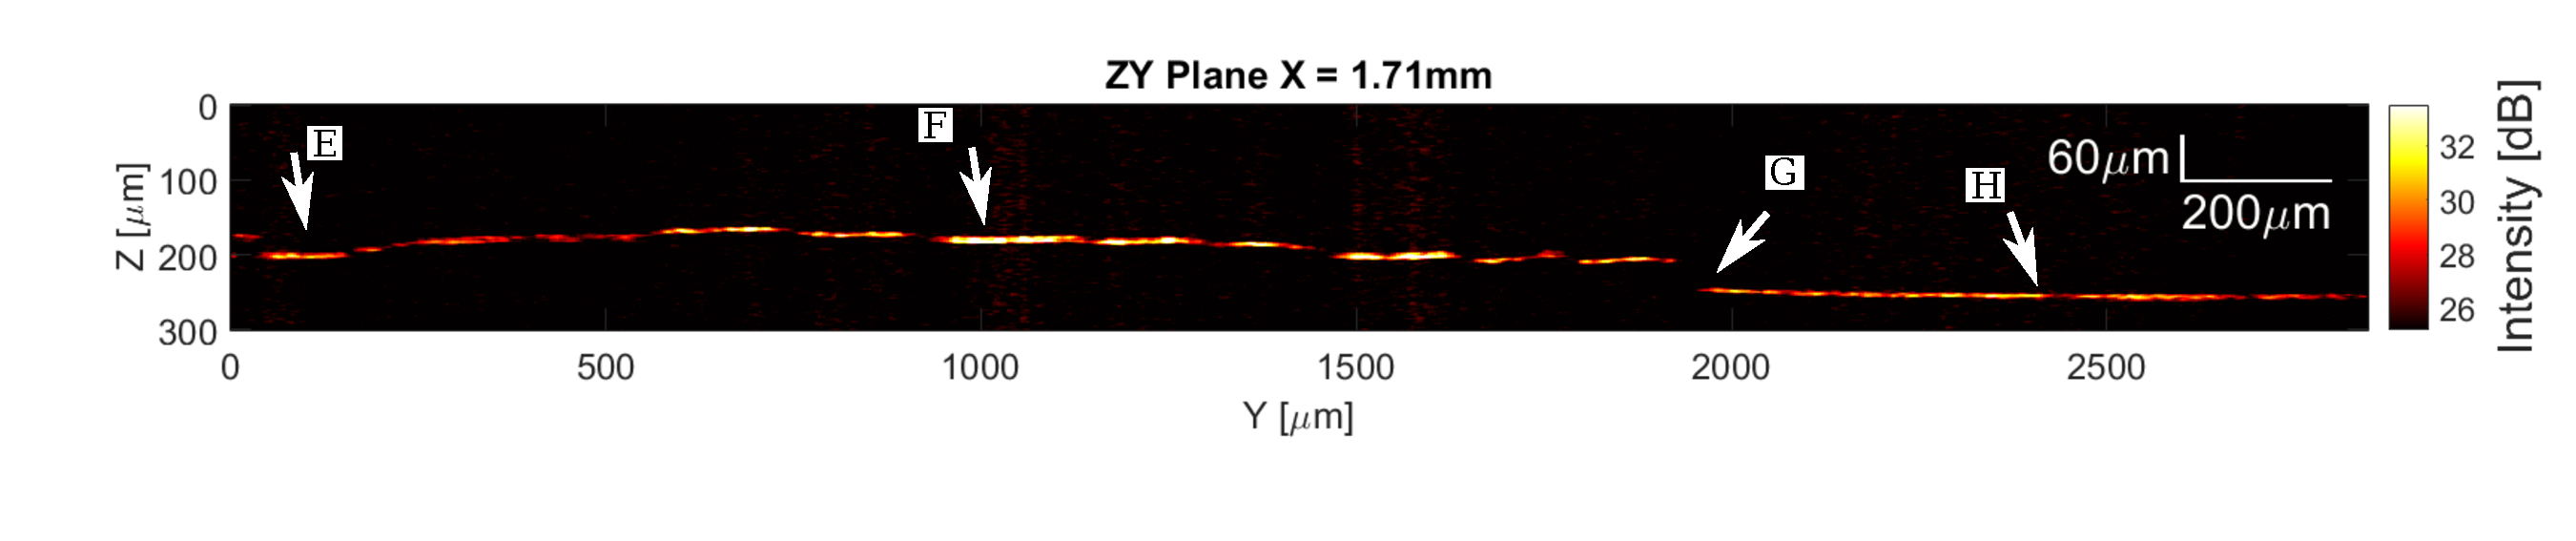
\includegraphics[width=1\linewidth]{img/chap2/ZYPlane_moneda}}
	\caption[Secciones transversales de la moneda]{Planos $ZX$ y $ZY$ reconstruidos a partir de OCT para la moneda, estos corresponden a la sección transversal. La presencia de una sola línea está asociada a que solo hay un reflector en la moneda.}
	\label{fig:monedabscan}
\end{figure}

A partir de los datos obtenidos, se realizó una reconstrucción tridimensional del volumen de datos, una secuencia de perspectivas de la topografía obtenida para la moneda a partir de este procedimiento, se encuentra en la Fig.~\ref{fig:PerspectivasTopologia}.

%En la sección transversal se distinguen estructuras regiones, tales como la zona plana de la moneda en la parte superior ($X\approx 0-200\mu m$) y las alas a lo largo del eje $X$ ($X\approx 800-2000\mu m$). Las secciones del escaneo B que aparecen oscuras, corresponden a aquellos puntos en la moneda que esparcieron más de lo reflejado, como las transiciones entre regiones a diferentes alturas (las alas, la cabe y las hojas). En la Fig.\ref{subfig:ZYPlane_moneda}, se muestra un corte de la moneda en la dirección $ZY$ en $X = 1.71mm$, de manera similar a la imagen anteriore, se observan zonas rectas ($Y \approx  2000\mu m-2500\mu m$) y con relieve en la moneda ($Y \approx  500\mu m-1700\mu m$). 



\begin{figure}
\centering
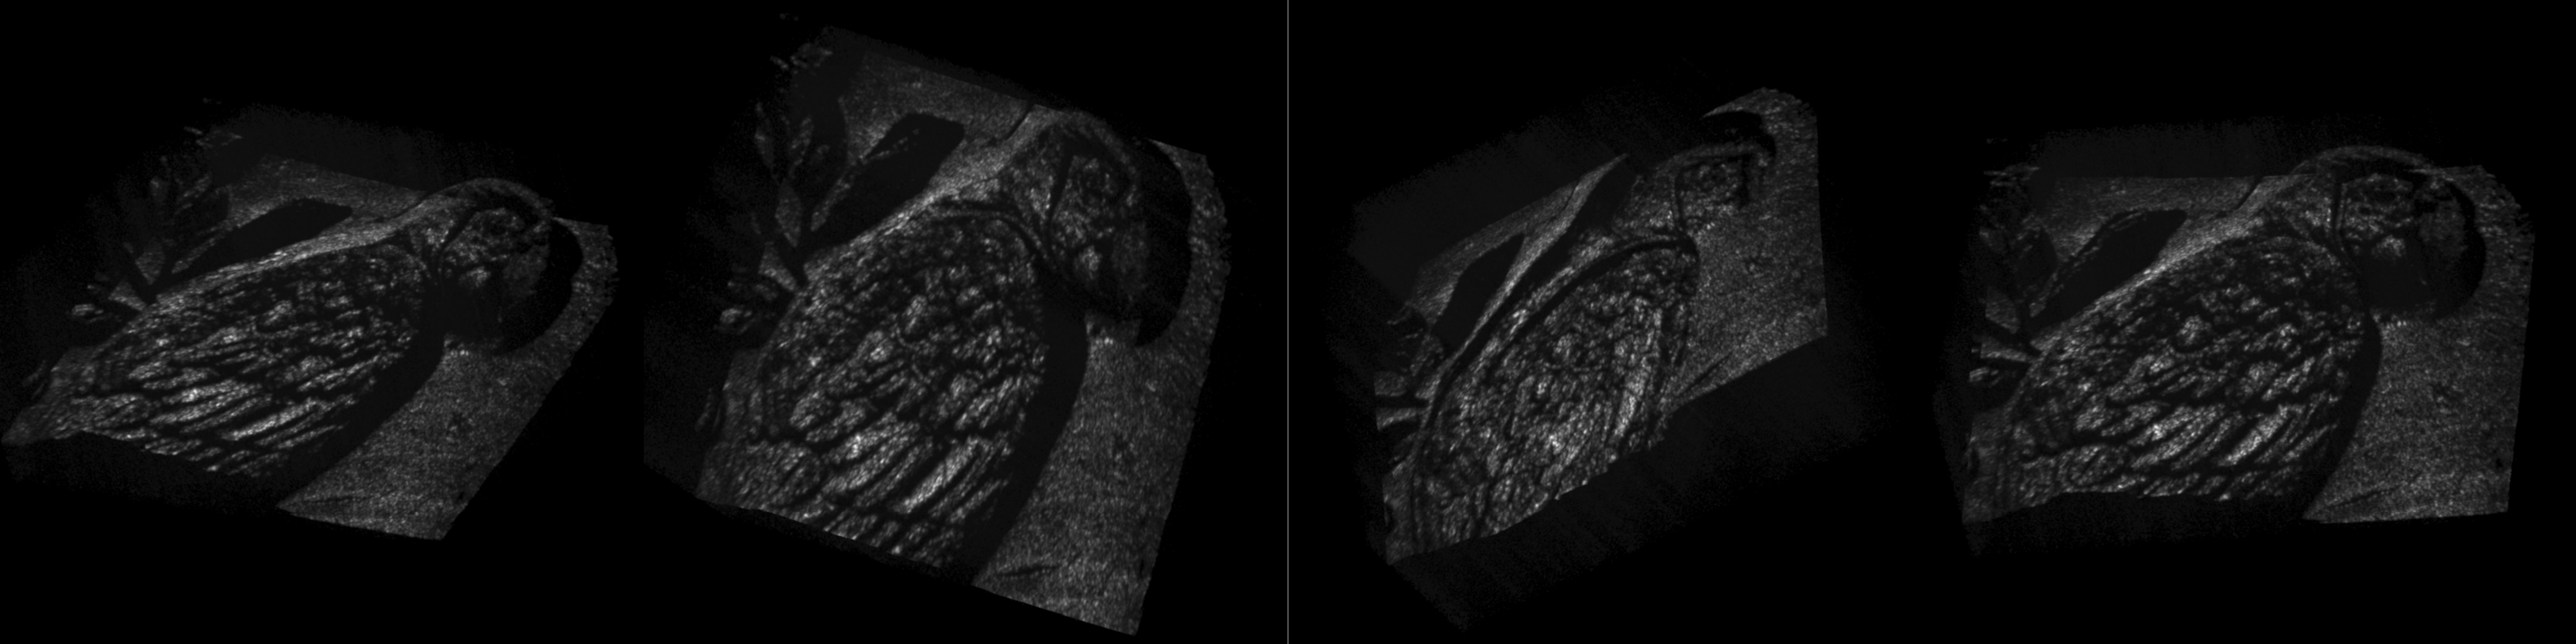
\includegraphics[width=1\linewidth]{img/chap2/PerspectivasTopologia}
\caption[Perspecivas de la topografía de la moneda.]{Secuencia de perspectivas de la topografía de la moneda reconstruidas con OCT.}
\label{fig:PerspectivasTopologia}
\end{figure}

\newpage

\subsubsection{Estructura ala de \textit{Blattodea}}


La segunda muestra que se analizó es un ala \exvivo de un insecto de la familia \emph{blattodea}, correspondiente al ala frontal conocida como \emph{tegmen}. El \emph{tegmen} en general se encuentra altamente esclerosado, es decir, endurecido por las estructuras que la conforman y la función que cumple, siendo esta última, ayudar durante el vuelo del insecto y servir como protección cuando todas las alas se encuentran plegadas. El ala empleada en las mediciones se presenta en la Fig.~\ref{fig:blattoawingzoomed}, el área que se encuentra señalada con línea punteada roja corresponde a la región de la cual se obtuvieron las imágenes. La vena más grande que se muestra en el área central de la imagen punteada y de la cual se ramifican venas más pequeñas, se conoce como \emph{radio}. El \emph{radio} cumple la función de dar el principal soporte al ala, pues contiene musculatura que ayudan a la oscilación durante el vuelo. La muestra se colocó en un portamuestras traslucido mediante un protector adhesivo.

\begin{figure}[h!]
	\centering
	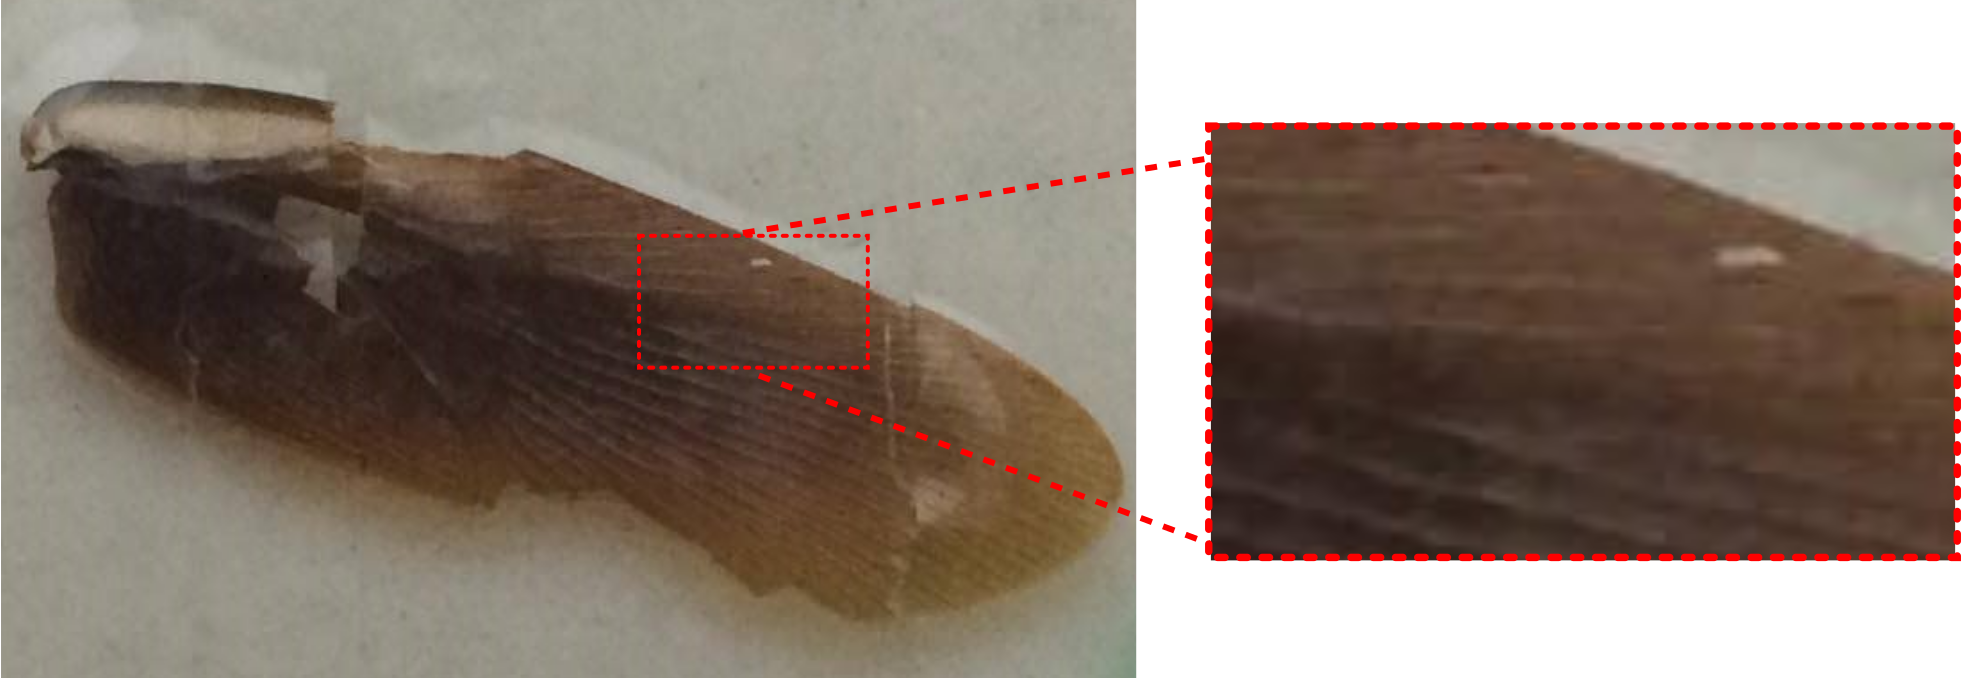
\includegraphics[width=0.7\linewidth]{img/chap2/BlattoaWingZoomed}
	\caption[Ala frontal o \emph{tegmen} de \emph{blattodea}.]{Ala frontal o \emph{tegmen}de \emph{blattodea} empleada en las mediciones. A la izquierda, fotografía de la ala, a la derecha, región a analizar.}
	\label{fig:blattoawingzoomed}
\end{figure}

De manera similar al proceso realizado para la moneda, se capturaron ocho patrones de interferencia con saltos de fase aleatorios, de forma que la modulación se recuperó a través del IPS con desplazamientos de $1\mu m$, a lo largo de una profundidad de $500\mu m$. La proyección \enface de todas las profundidades se presenta en la Fig.~\ref{fig:OCT_projection_points}, esta imagen permite distinguir algunas estructuras del ala, señaladas con flechas desde la $A$ hasta la $I$. El punto $A$ corresponde a una región en donde se observa el portamuestras, $B$ e $I$ corresponden a lugares en los cuales hay proyector adhesivo, $C$ es una vena ubicada en $X\approx 500\mu m$ aparece como una región más oscura, ya que la cantidad de luz absorbida por este tipo de estructuras se espera que sea alta; $D$ es una región de la membrana del ala y es por ello que aparece como una zona brillante, en donde la luz es altamente reflejada. $E$ aparece como una región oscura pues en esa zona la mayor parte de la luz fue absorbida por el ala, $F$ muestra un punto ubicado en el \emph{radio} del ala, y $H$ corresponde a la transición entre el ala y aire. Si se realizan dos cortes transversales a lo largo de las líneas punteadas en $X=0.6mm$ y $Y=1.72mm$, como se muestra en la Fig.\ref{fig:OCT_projection_points}, las secciones transversales con los puntos descritos anteriormente pueden analizarse desde la profundidad de la imagen, como se indican en la Fig.\ref{fig:blattodeaplanos}.
% VENA CENTRAL CORRESPONDE AL RADIO, EL BORDE DEL ALA SE CONOCE COMO COSTA, EL ALA QUE TENEMOS ES EL TEGMEN O ALA FRONTAL, EN GENERAL ESCLEROSADA (ENDURECIDA), SIRVE PARA VOLAR ASÍ COMO PROTECCIÓN PARA LAS ALAS CUANDO LAS TIENE REPLEGADAS
% IMAGEN DE COMPARACIÓN
%\begin{figure}
%	\centering
%	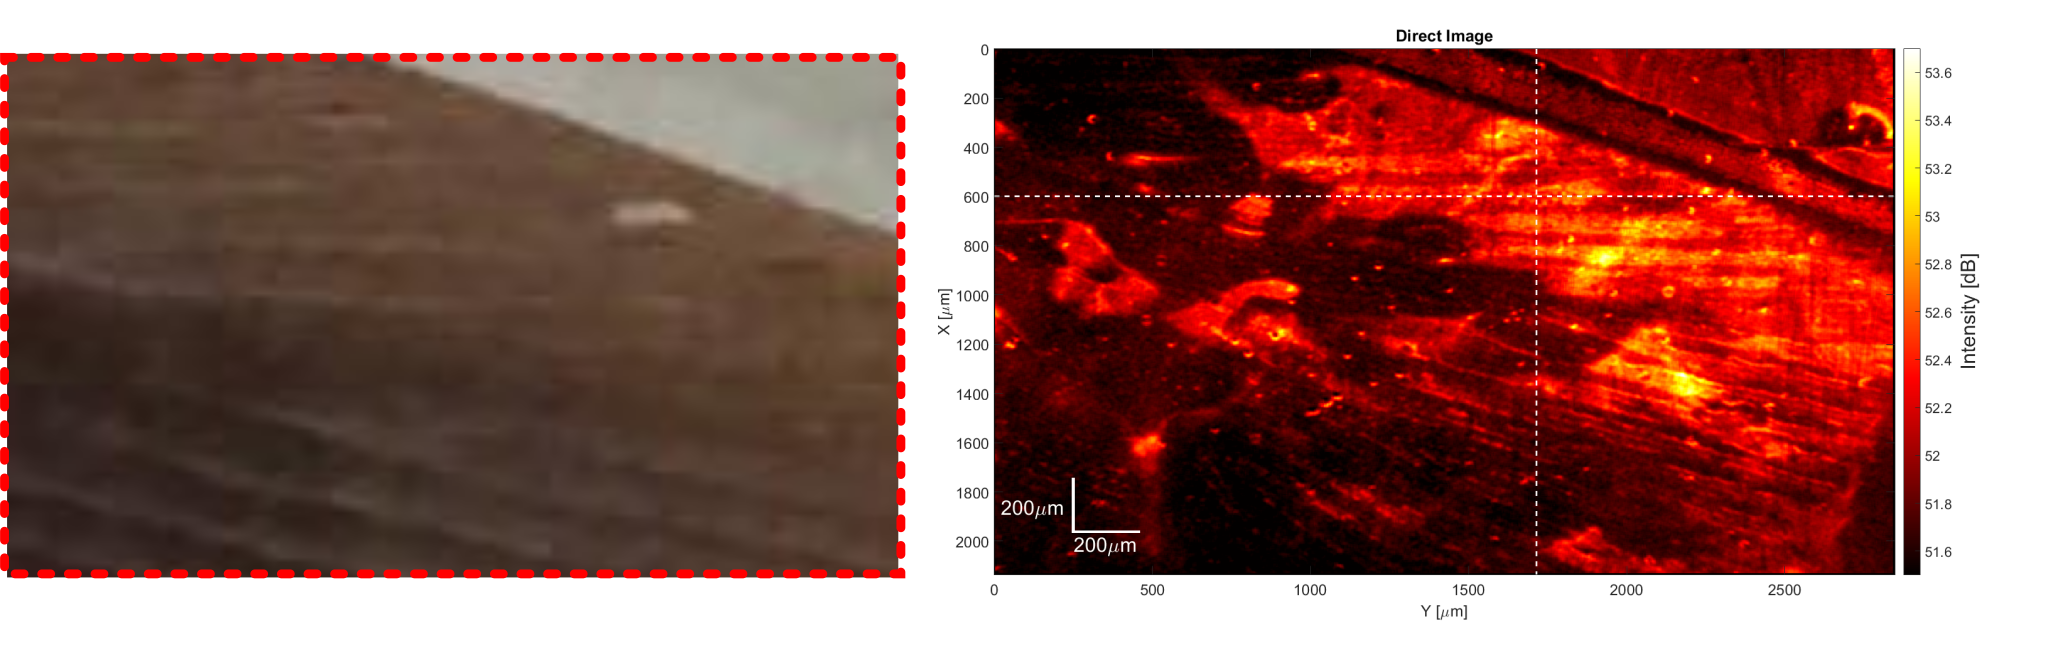
\includegraphics[width=1\linewidth]{img/chap2/WingComparisonDirect_2}
%	\caption[Imagen directa recuperada con OCT.]{Imagen directa recuperada con OCT comparada contra la región del ala analizada. Esta imagen corresponde a la superposición de todas las imágenes en profundidad obtenidas.}
%	\label{fig:wingcomparisondirect}
%\end{figure}
% UNICAMENTE INMAGEN DIRECTA
\begin{figure}[h!]
	\centering
	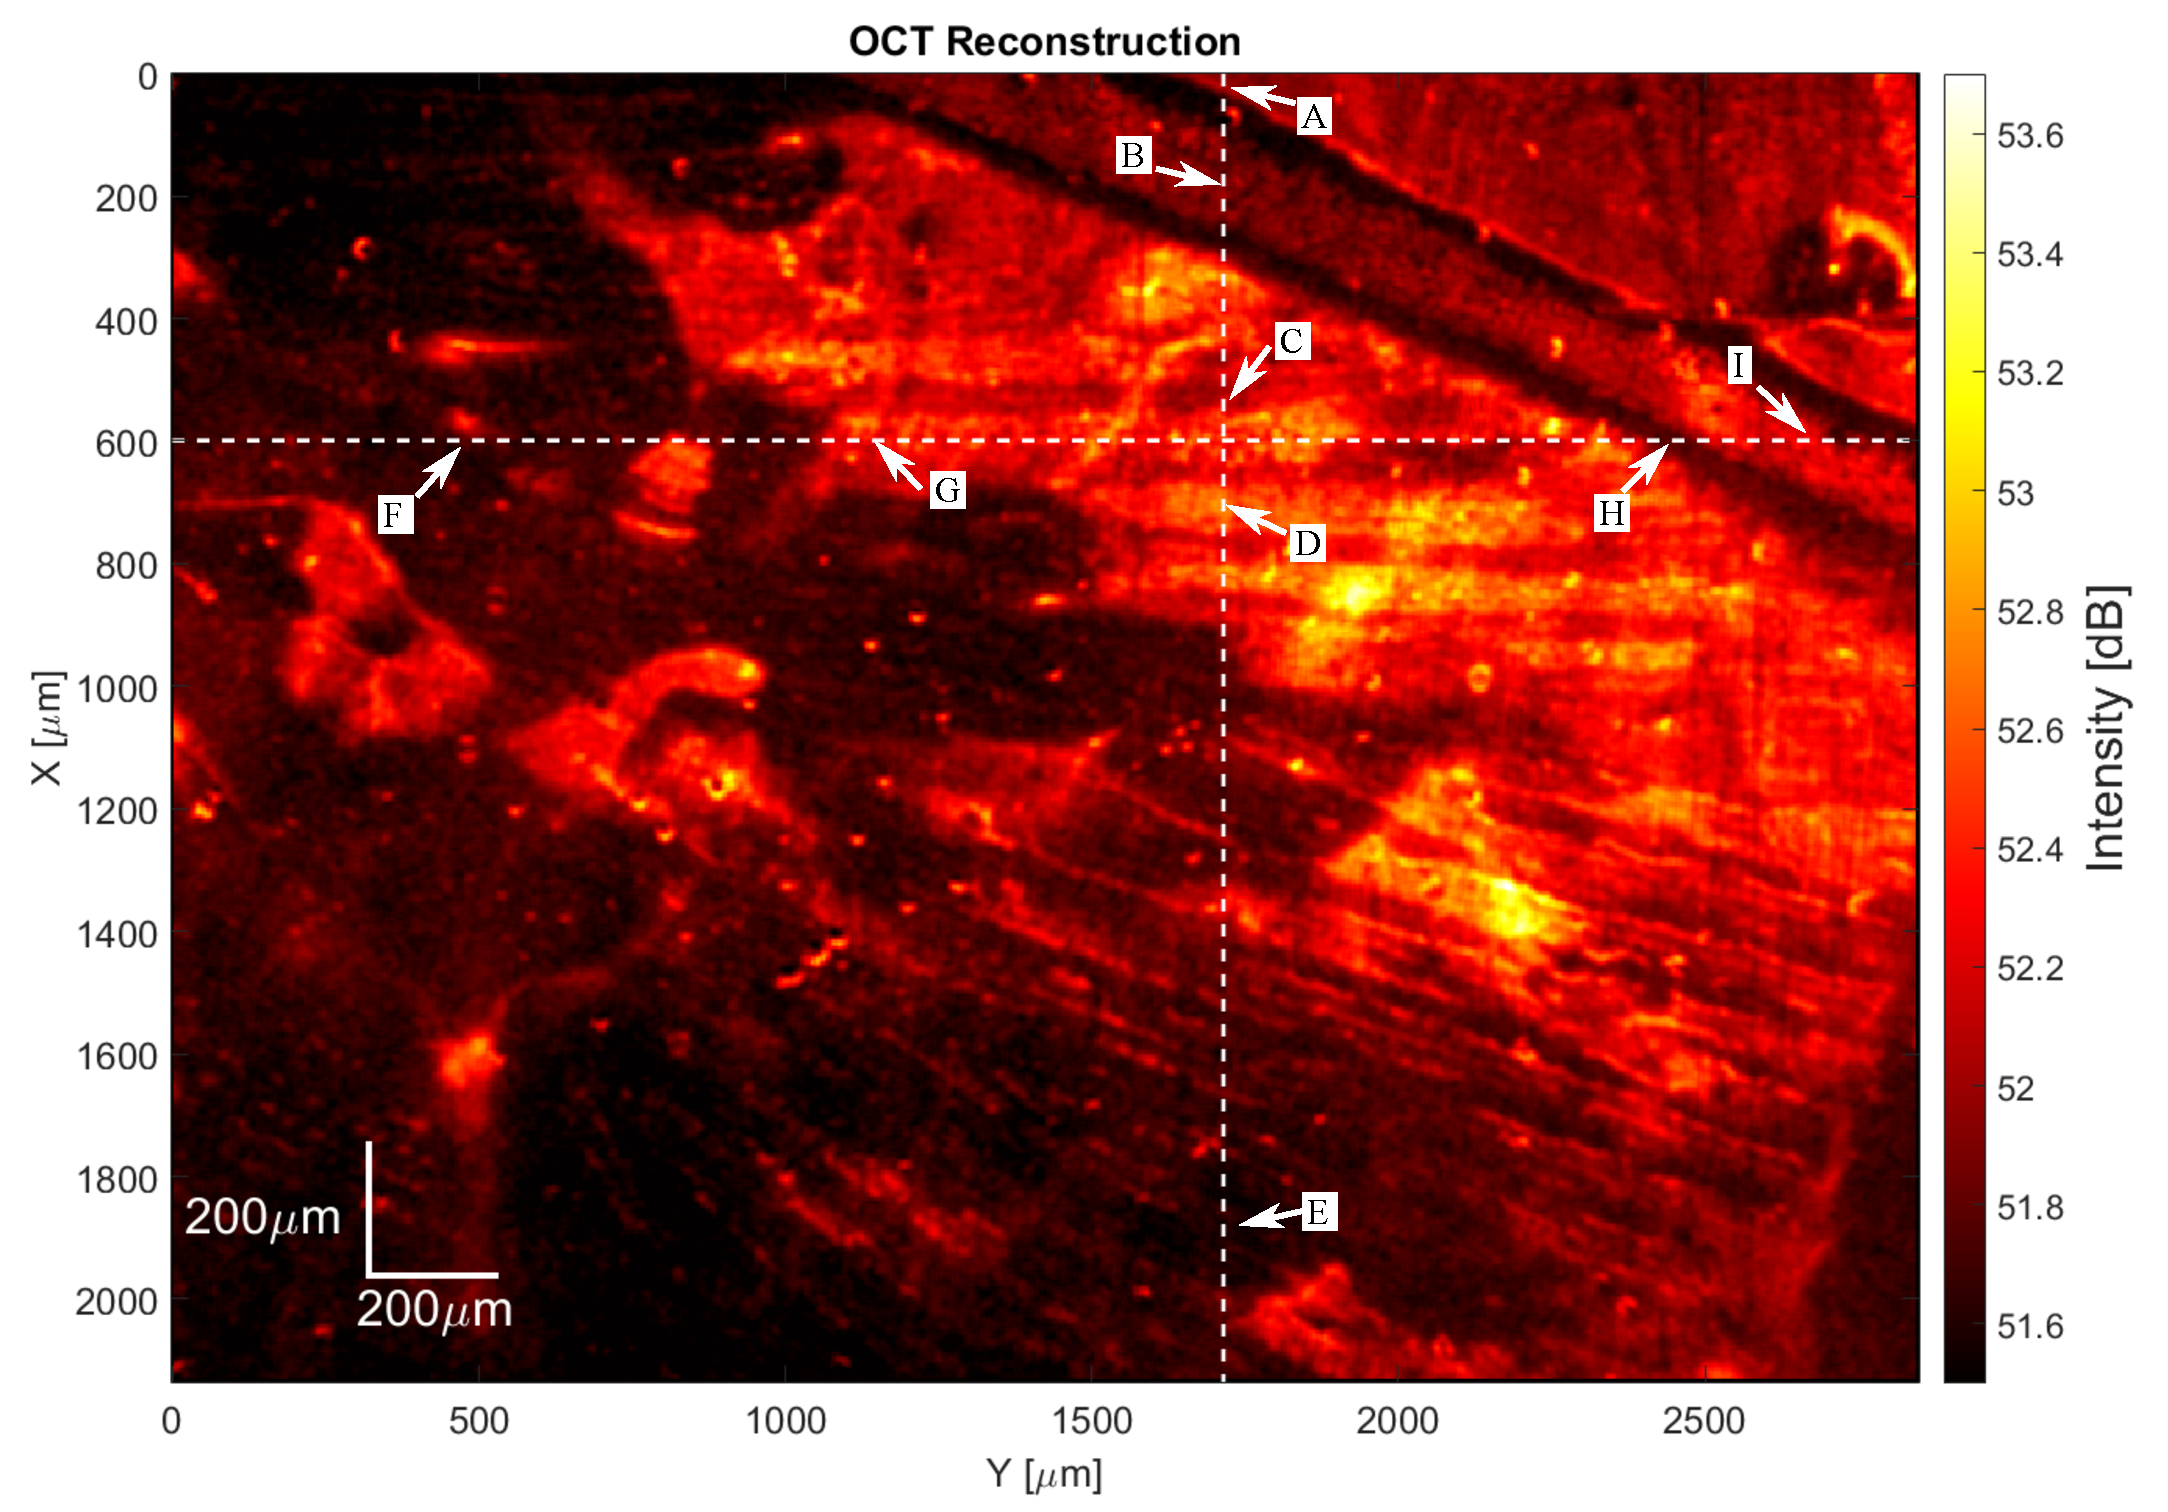
\includegraphics[width=0.7\linewidth]{img/chap2/OCT_projection_points}
	\caption[Imagen recuperada con OCT del ala de \textit{blattodea}.]{Imagen directa recuperada con OCT. Esta corresponde a la suma de todas las imágenes en profundidad obtenidas. Los puntos marcados son zonas de interés que se discuten en el texto. La imagen tiene un color falso de $51.5$ a $53dB$.}
	\label{fig:OCT_projection_points}
\end{figure}

%, estos dos puntos aparecen en la imagen ya que como se expicó en la Sección~\ref{sec:OCT_Esquema}, OCT registra los cambios en el índice de refracción del medio
La imagen correspondiente a la Fig.~\ref{subfig:Bscan_Wing} es el plano $ZX$ en $Y=1.72mm$, correspondiente a un escaneo tipo B para el ala, los puntos $A-E$ descritos anteriormente se han ubicado en la figura. Los puntos $PA1$ y $PA2$ refieren a la primer y segunda superficie del protector adhesivo, en general son altamente brillantes, ya que este material refleja una gran porción de la luz, y adicionalmente es la primer superficie que encuentra la luz. La región $RA$ corresponde a la ubicación del \emph{radio} del ala, y se espera que sea una región oscura porque como lo mostraba la imagen directa, ésta absorbe fuertemente la luz. Los puntos oscuros ubicados a lo largo del eje $X$ y denotados como $VA$ son venas del ala, estos puntos reflejan menos luz que la membrana dadas sus características, y por ende parecen lugares oscuros. La membrana del ala por su parte, es una estructura delgada que refleja de manera especular una alta porción de la luz, y es por ello que aparece como puntos altamente brillantes, están indicados como $ME1$ y $ME2$ para indicar la primera y la última superficie de la membrana. La línea continua indicada como $PM$ es el portamuestras sobre el que se encuentra posicionado el ala, el motivo de que no se encuentre completamente continuo se debe a que las venas atenúan fuertemente la luz, y debajo de éstas áreas es baja la reflexión. Sin embargo, nótese que por debajo del \emph{radio} ($X\approx 0.9mm$) se observa el portamuestras, es decir, aunque hayan puntos que producen sombras por la luz que atenúan, si hay una fracción de luz que penetre es posible obtener imagen de estructuras por debajo de las capas superficiales.

\begin{figure}[ht!]
	\centering
	\subfigure[Plano $ZX$ o escaneo B obtenido para el \emph{tegmen}.]{\label{subfig:Bscan_Wing}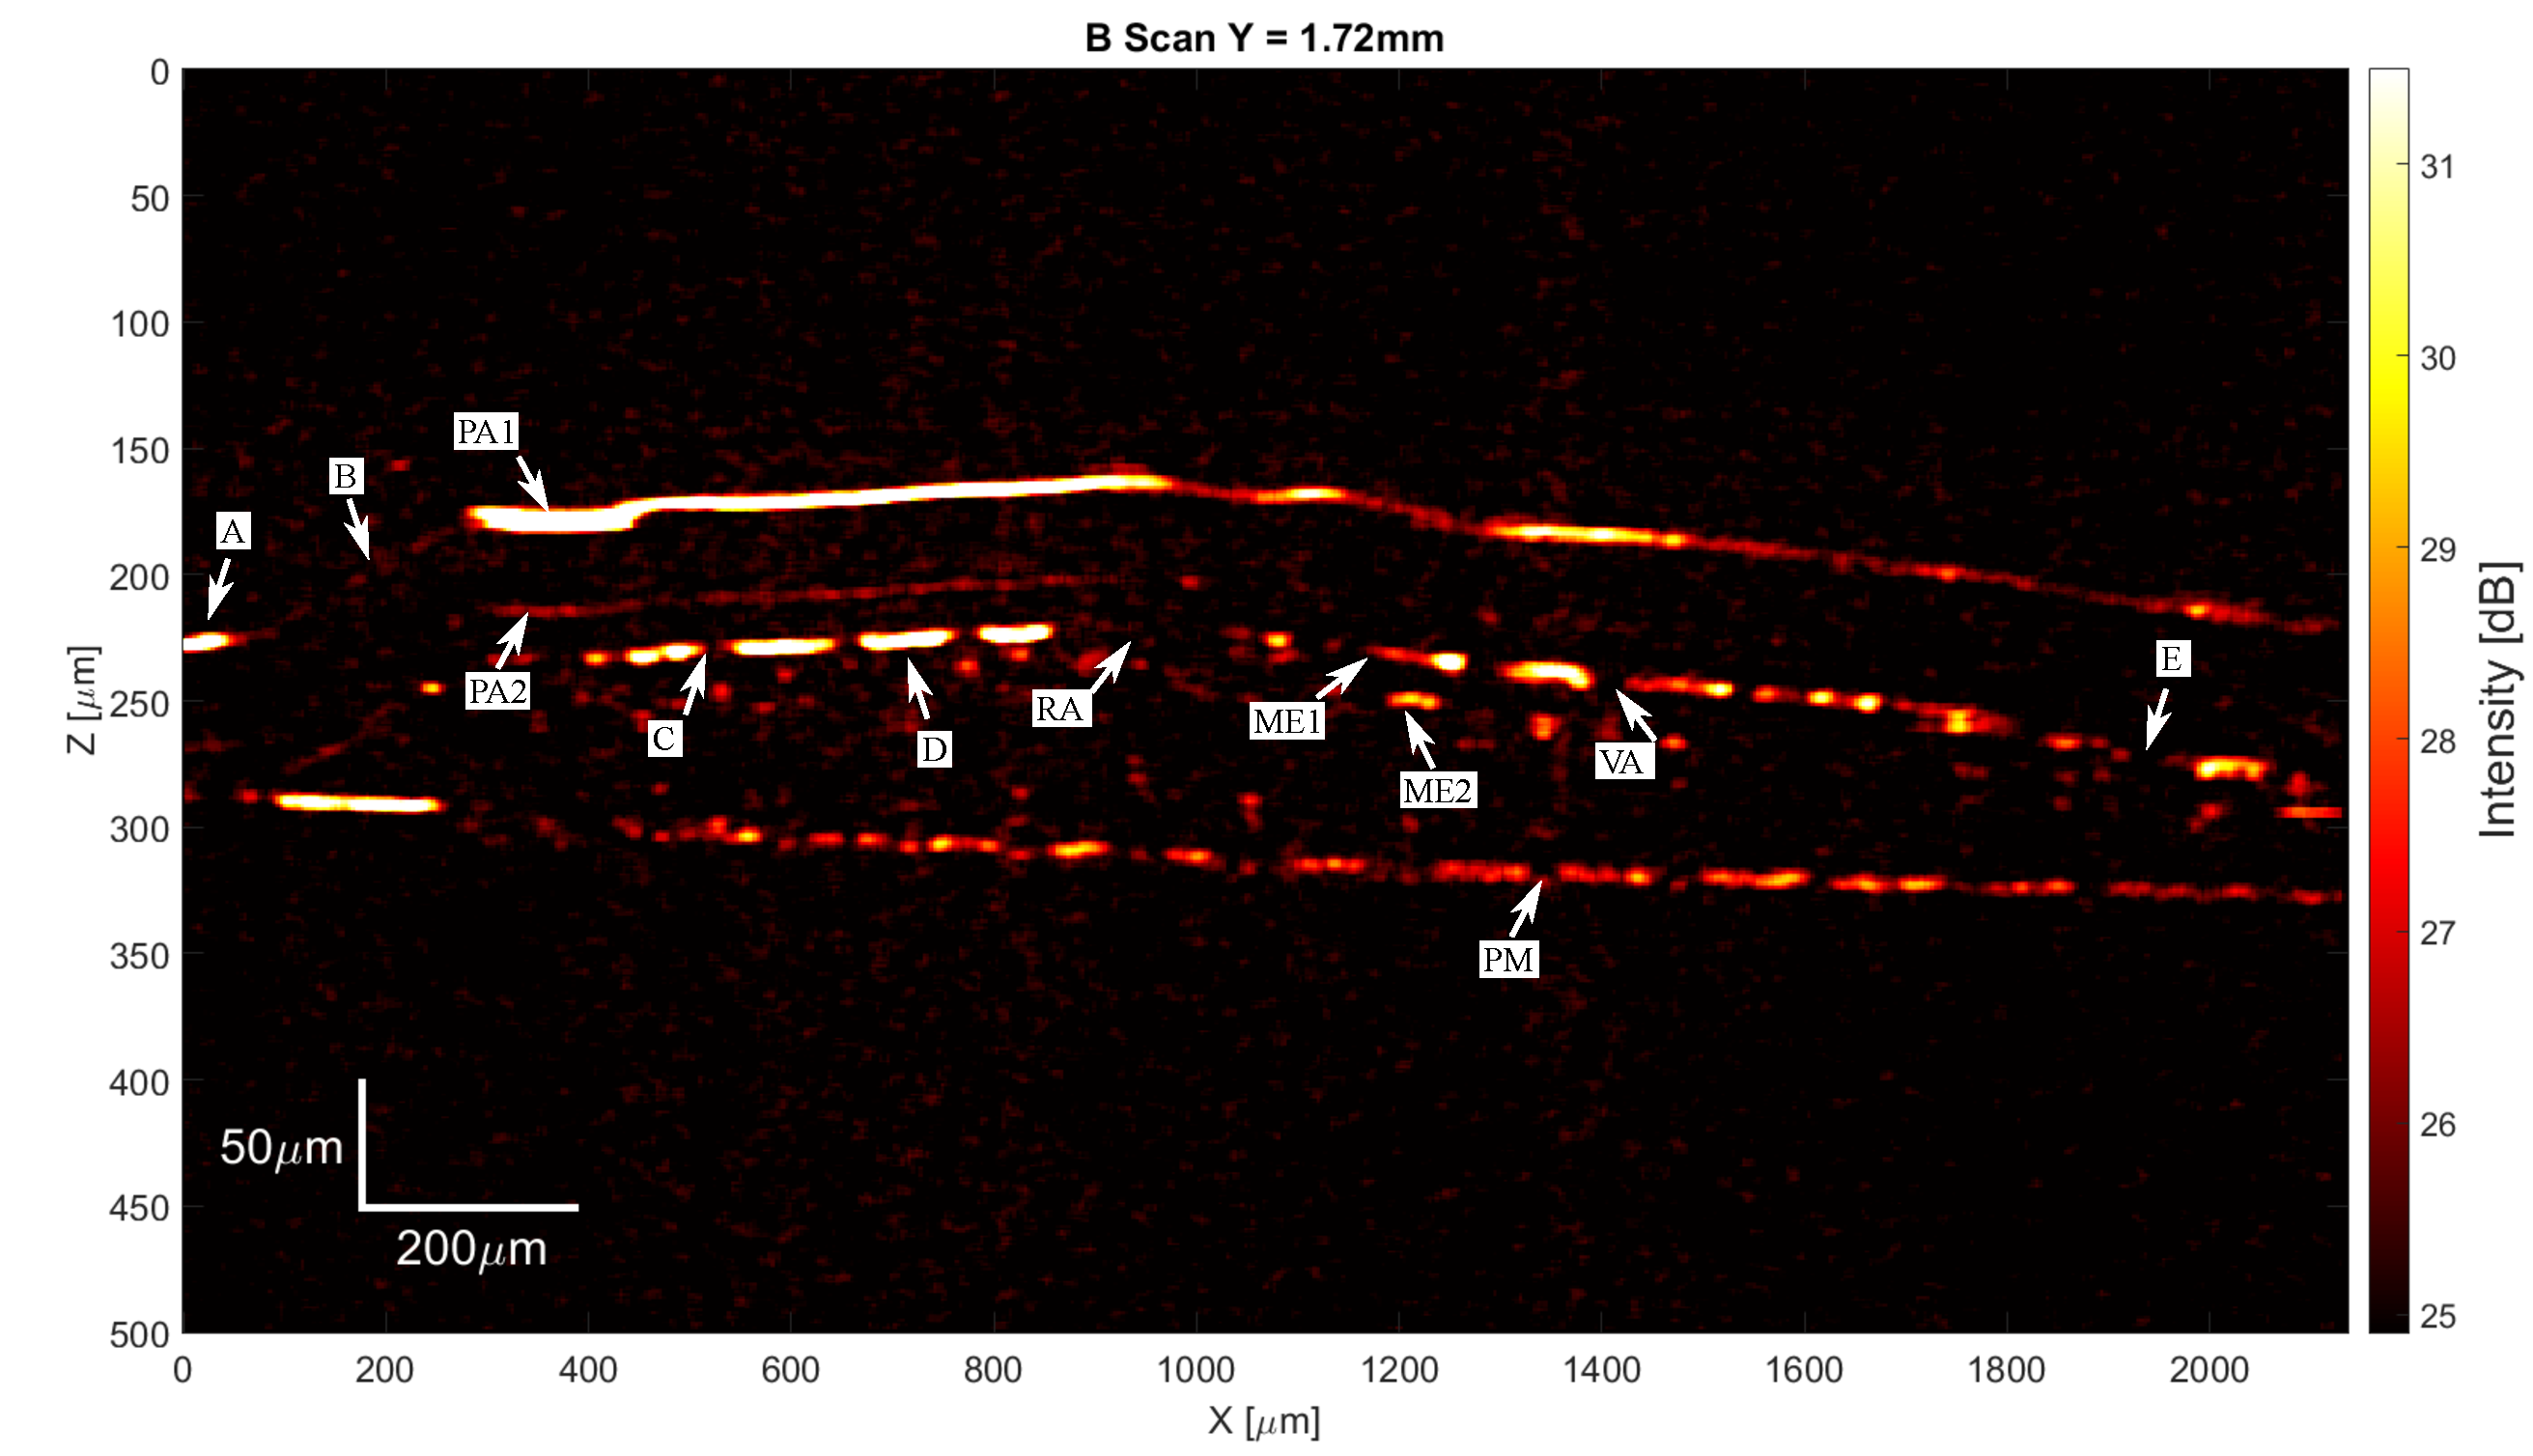
\includegraphics[width=0.8\linewidth]{img/chap2/Bscan_Wing}}
	\subfigure[Plano $ZY$ reconstruido para el \emph{tegmen}.]{\label{subfig:ZY_Wing}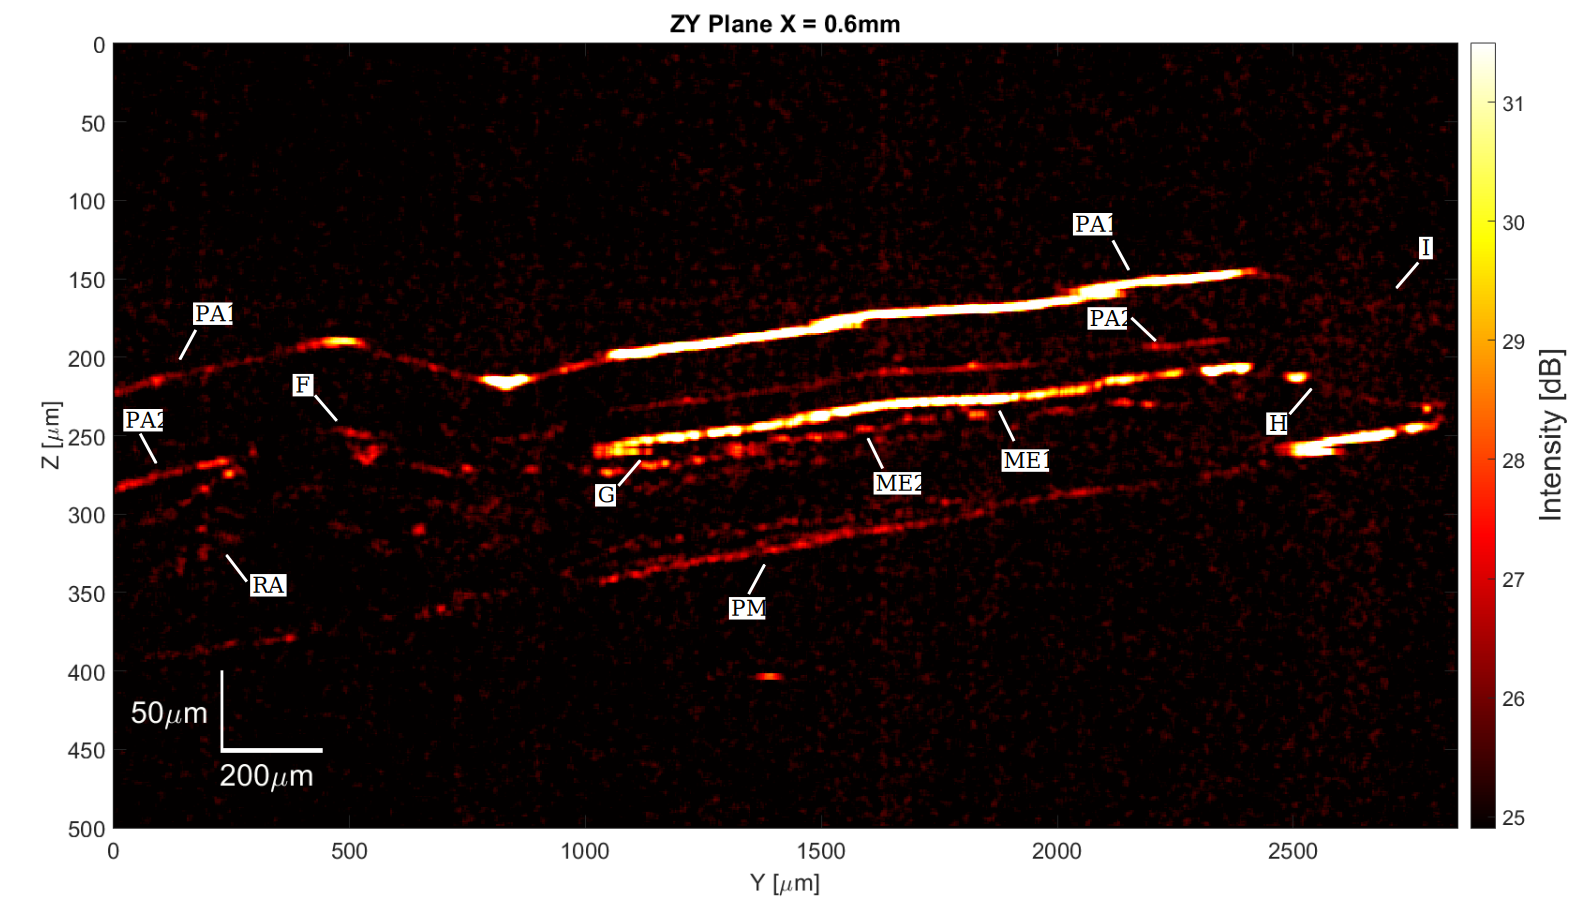
\includegraphics[width=0.8\linewidth]{img/chap2/ZY_Wing}}
	\caption[Planos de las secciones transversales del ala de \textit{blattodea}]{Planos de las secciones transversales en $ZX$ y $ZY$ reconstruidos con OCT para el \emph{tegmen}. Las imágenes tiene un color falso con un rango de $25$ a $32dB$. Los puntos indicados corresponden a: $PA1$ y $PA2$ primera y segunda superficie del protector adhesivo respectivamente, $RA$ vena correspondiente al radio de la ala, $PM$ placa portamuestras, $VA$ vena ramificada a partir del radio, $ME1$ y $ME2$ corresponden al inicio y fin de la membrana de la ala respectivamente.}
	\label{fig:blattodeaplanos}
\end{figure}

El punto $A$, indicado anteriormente, muestra una región plana de la imagen directa, si se observa este punto en la sección transversal, se aprecia que en realidad está conformado por tres capas, dos de ellas correspondiente al protector adhesivo y la última por el portamuestras. El punto $B$, conformado por las mismas capas anteriores, tiene una menor intensidad sobre el adhesivo, ya que este se encuentra inclinado con respecto al plano del detector, no obstante, el portamuestras que se encuentra alineado con el detector presenta una intensidad mucho mayor. $C$ muestra una de las diferentes venas derivadas del \emph{radio} que aparecen como puntos oscuros. $D$ está ubicado sobre una sección del ala con membrana, la que aparece como un punto brillante por la cantidad de luz que refleja. $E$ es una región oscura ya que por esa zona empieza a aparecer la región del \emph{radio}.

La Fig.~\ref{subfig:ZY_Wing} es la sección transversal del plano $ZY$ ubicado en $X=0.6mm$. El escaneo en este caso se encuentra alineado con una región de la membrana del ala, es por ello que aparece una línea que muestra claramente las dos superficies del ala $ME1$ y $ME2$. Adicionalmente, se observa como el \emph{radio} $RA$ se encuentra entre el portamuestras y el protector adhesivo, y la forma que siguen los músculos del ala. Por ejemplo en $Y\approx 1-1000\mu m$ se aprecia que el ala no se encuentra completamente alineada con el portamuestras. En este caso, no se aprecia ninguna vena por que nos encontramos en un plano paralelo que se encuentra sobre la membrana, una imagen similar a ésta se obtiene en el volumen de datos, pero mostrando la sección transversal de las venas.

Los puntos $F-I$ ubicados a lo largo del eje $X$, aparecen en este caso mostrando algunas regiones de interés. $F$ indica una región brillante sobre el \emph{radio}, bajo la cual se aprecia un pliegue del ala, y como se ve en la proyección \enface, capas más internas como el portamuestras son mucho menos visibles dada la absorción que tiene esta región. El punto $G$ está indicando la transición entre el \emph{radio} y la membrana del ala, y es por ello que aparece el cambio en el contraste. $H$ corresponde a la transición entre el ala y el portamuestras, esto se evidencia por la desaparición de la alta intensidad sobre la membrana para estar ubicada sobre el portamuestras. En el punto $I$ se observa la región donde solo el protector adhesivo y el portamuestras reflejan luz.
%El escaneo tipo B muesta varias características que con el experimento de la moneda no eran evidentes, primero que todo, en el caso del ala, se nota la presencia de múltiples reflectores a distintas profundidades para un punto específico, por ejemplo, en $X\approx 0.6mm$ se aprecia la reflexión de diferentes capas. Un ejemplo de esto, son la primer y segunda superficie del protector adhesivo $PA1$ y $PA2$ respcectivamente. 
De los resultados obtenidos, también se realizó una reconstrucción tridimensional de la estructura del ala, una secuencia de perspectivas de los resultados para el ala se presenta en la Fig.~\ref{fig:perspectivaswing}

\begin{figure}[!h]
	\centering
	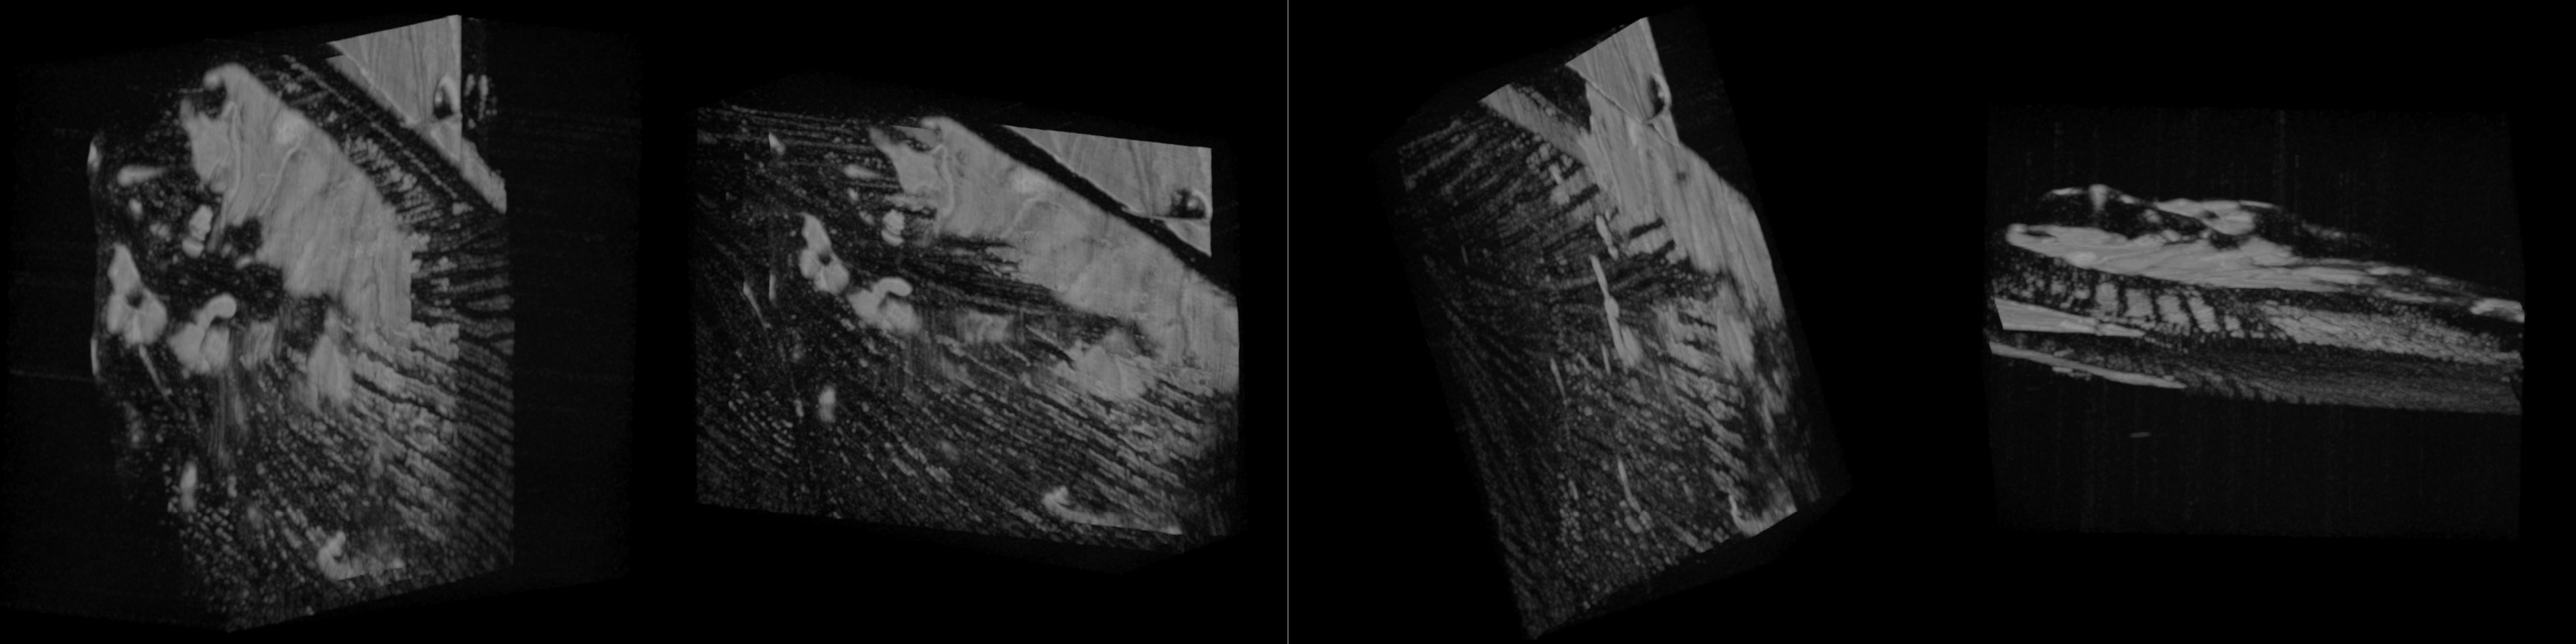
\includegraphics[width=1\linewidth]{img/chap2/Perspectivas_wing}
	\caption[Perspectivas del ala de \textit{blattodea}.]{Secuencia de perspectivas de la reconstrucción del ala.}
	\label{fig:perspectivaswing}
\end{figure}


\bibliographystyle{unsrt}
\bibliography{ref/Ref_chap_2}
\chapter{Supresión del ruido por \textit{speckle} en imágenes de OCT}
\label{chapter:supresion_ruido_en_oct}

Uno de los principales problemas que tienen las imágenes provenientes de OCT, es que en la mayor parte de los casos se encuentran afectadas por la presencia de ruido de \textit{speckle}. El objetivo de este capítulo es proponer un método de filtrado que preserve las estructuras que se miden con OCT, pero que permita mitigar los efectos del ruido y faciliten la comprensión de la información que poseen las imágenes. Para tal fin, se propone una modificación y extensión de un algoritmo conocido como \textit{non-local means}, considerando las características de la información disponible en OCT. 

El propósito de este capítulo es dar las bases fundamentales para comprender la naturaleza del filtrado propuesto y relacionarlo con los resultados obtenidos. En ese orden de ideas, este capítulo se encuentra dividido en cinco secciones, en donde se analizarán los siguientes aspectos: la Sección~\ref{sec:principios_estadistica_speckle} corresponde a las bases de la estadística de \textit{speckle} de primer orden; la Sección~\ref{sec:estado_arte_filt_speckle} presenta el estado del arte del filtrado de ruido por \speckle en imágenes de OCT; la Sección~\ref{sec:caracteristicas_speckle} discute las causas de la aparición de \speckle en el caso de OCT, fundamento con el que será posible entender la técnica de filtrado que se quiere implementar, y que se discute en la Sección~\ref{sec:from_SAR_to_OCT}. En la última Sección~\ref{sec:resultado_filtrado} se mostrará un análisis de los resultados obtenidos con el filtrado propuesto, y se analizarán algunas aplicaciones en donde se ha probado .

\section{Principios básicos de la estadísticas de \textit{speckle}}
\label{sec:principios_estadistica_speckle}

El \textit{speckle} fue descubierto durante las primeras pruebas realizadas con láseres, en donde se apreciaba la formación de un patrón granulado cuando el haz de luz se reflejaba en superficies tales como las paredes del laboratorio. A partir de estas observaciones, se explicaría que el \speckle surge cuando luz coherente se refleja en una superficie cuya rugosidad se encuentra en la escala de la longitud de onda, o bien, cuando la luz se propaga por un medio con variaciones aleatorias en el índice de refracción \cite{Goodman2010,Dainty1975}. El patrón obtenido bajo estas condiciones posee un alto contraste, con estructuras granulares finas y distribuido en el espacio de una manera relativamente uniforme. La formación de patrones de \speckle es un fenómeno aleatorio, en el que no es posible describir con exactitud en qué lugares aparecerá una estructura brillante u oscura, esto se debe a que la mayor parte de los materiales poseen una rugosidad aleatoria en la escala micro, y su comportamiento no puede ser descrito de manera determinista, sino que debe tratarse mediante funciones de probabilidad que describen las características del campo de \textit{speckle}. Las variaciones aleatorias que son inducidas en el haz para formar patrones de \textit{speckle} en general son complejas, por ende, poseen una amplitud y una fase que representan una magnitud y una dirección aleatoria respectivamente \cite{Goodman1976}. La superposición de las amplitudes y fases aleatorias de todos los puntos luego de la reflexión en la superficie, dan lugar a la formación del patrón de \textit{speckle}. Esta suma produce que la amplitud y la fase sean aleatorias, y de acuerdo a la diferencia de fase que haya entre los puntos en la superficie o las contribuciones elementales se producirá interferencia constructiva o destructiva, por lo tanto el \speckle tendrá una apariencia de puntos brillantes u oscuros respectivamente.


%El \textit{speckle} fue descubierto durante las primeras pruebas realizadas con láseres, en donde se apreciaba la formación de un patrón granulado cuando el haz de luz se reflejaba en superficies tales como las paredes del laboratorio. A partir de estas observaciones, se explicaría que el \speckle surge cuando luz coherente se refleja en una superficie cuya rugosidad se encuentra en la escala de la longitud de onda, o bien, cuando la luz se propaga por un medio con variaciones aleatorias en el índice de refracción \cite{Goodman2010,Dainty1975}. El patrón obtenido bajo estas condiciones posee un alto contraste, con estructuras granulares finas y distribuido en el espacio de una manera relativamente uniforme. Dado que la rugosidad que poseen la mayor parte de los materiales es aleatoria, el patrón de \speckle obtenido sigue también una forma aleatoria, por lo que sus características deben describirse como funciones de probabilidad que relacionan las propiedades del campo de \speckle. Las variaciones aleatorias que son inducidas en el haz para los patrones de \speckle son, en general, complejas, por lo tanto, poseen una amplitud y una fase, representando una magnitud y una dirección aleatoria respectivamente \cite{Goodman1976}. El patrón de \speckle formado posee entonces la superposición de todas las contribuciones elementales al campo luego de la reflexión en la superficie, esta superposición produce que la amplitud y la fase sean aleatorias, y de acuerdo a la diferencia de fase que haya entre las contribuciones elementales, se formará dará interferencia constructiva o destructiva y como consecuencia de esto, el patrón de \speckle tiene una apariencia de puntos brillantes y oscuros distribuidos en el espacio.

%La superposición o suma de todas las contribuciones del campo complejo luego de reflejarse en la superficie producen un patrón de interferencia constructiva o destructiva, apareciendo como puntos brillantes u oscuros. 


%El \textit{speckle} surge cuando luz coherente es reflejada por una superficie cuya rugosidad se encuentra en la escala de la longitud de onda, o bien cuando la luz se propaga por un medio con variaciones aleatorias del índice de refracción\cite{Goodman2010,Dainty1975}. El patrón que se obtiene bajo estas condiciones posee un alto contraste con estructuras finas granulares y distribuido de una forma relativamente uniforme. Las primeras observaciones de patrones de \speckle se dieron con la aparición de los primeros láseres, ya que luego de esto interactuar con superficies que en la escala macro parecen lisas, pero que desde una perspectiva microscópica son rugosas. Debido a que la rugosidad que poseen la mayor parte de los materiales es aleatoria, el patrón de \speckle obtenido sigue también una forma aleatoria. Las variaciones que son introducidas en la luz, pueden ser complejas, con una amplitud y una fase que representan una longitud y una dirección aleatoria respectivamente. La superposición o suma de todas las contribuciones del campo complejo luego de reflejarse en la superficie producen un patrón de interferencia constructiva o destructiva, apareciendo como puntos brillantes u oscuros. 

Debido a que no se conocen detalles sobre la estructura microscópica de la superficie, es más fácil analizar las características de los patrones de \speckle de manera estadística \cite{Dainty1975}, asumiendo que sus propiedades en la escala microscópica difieren. Si $\boldsymbol{A}(x,y,t)$ es una señal compleja en el patrón de \textit{speckle} en un punto $(x,y)$ en un instante $t$, ésta puede representarse como

%Debido a que no se conocen detalles sobre la estructura microscópica de la superficie, es más fácil analizar las características de los patrones de \speckle de manera estadística \cite{Dainty1975}, con esto, se asume que las propiedades en la escala macro de un objeto son iguales, pero difieren en la escala micro. Una señal compleja $\boldsymbol{A}(x,y,t)$ en un punto $(x,y)$ en un instante $t$, puede representarse como,

\begin{equation}
\boldsymbol{A}(x,y,t) = A(x,y,t)e^{i\theta(x,y,t)},
\end{equation}

\noindent donde $A(x,y,t)$ es la amplitud, $\theta(x,y,t)$ la fase y $(x,y,t)$ la dependencia espacial y temporal de dicha señal. El patrón de \speckle aparece cuando cada punto se encuentra descrito a través de la superposición de una gran cantidad de contribuciones elementales complejas $\boldsymbol{a_n}(x,y,t)$ con fases aleatorias provenientes de $N$ puntos diferentes y producidas por centros dispersores, de manera que el campo de \speckle obtenido corresponde a 

\begin{align}
\boldsymbol{A}(x,y,t) &= A(x,y,t)e^{i\theta(x,y,t)} \notag\\ 
&= \frac{1}{\sqrt{N}}\sum_{n=1}^{N} \boldsymbol{a_n}(x,y,t) \notag\\
&= \frac{1}{\sqrt{N}}\sum_{n=1}^{N} a_n(x,y,t) e^{i\phi_n(x,y,t)},
\end{align}

%\noindent donde $\boldsymbol{a_n}(x,y,t)$ es el n-enésimo punto contribuyente al campo, con amplitud $a_n(x,y,t)$ y fase $\phi_n(x,y,t)$. La estadística de \speckle busca describir el campo complejo $\boldsymbol{A(x,y,t)}$ a partir de cálculos estadísticos de la superposición de las contribuciones elementales, para describir así la probabilidad de que un punto en el espacio y tiempo posea una amplitud $A(x,y,t)$ y una fase $\theta(x,y,t)$. En los últimos dos parámetros se centrará el análisis, en base a las contribuciones elementales $a_n(x,y,t)$ y $\phi(x,y,t)$, por lo tanto se asumirá que \cite{Goodman2010}: (1) la amplitud $a_n$ y la fase $\phi_n$ de las contribuciones elementales, son estadísticamente independientes de $a_m$ y $\phi_m$ cuando $n\neq m$, es decir, la amplitud y la fase de las contribuciones elementales no aportan información sobre la amplitud y fase de otra contribución elemental diferente a sí misma; (2) para cualquier $n$ la amplitud $a_n$ y la fase $\phi_n$ son estadísticamente independientes, por lo tanto, conocer la amplitud $a_n$ no aporta información sobre la fase $\phi_n$ y viceversa; (3) las fases de las contribuciones elementales $\phi_n$ se encuentran distribuidas en el intervalo $(-\pi, \pi)$, esto es que la fase tiene la misma probabilidad de adquirir cualquier valor de fase en un rango de $2\pi$. 

\noindent donde $\boldsymbol{a_n}(x,y,t)$ es el n-enésimo punto contribuyente al campo, con amplitud $a_n(x,y,t)$ y fase $\phi_n(x,y,t)$. El campo complejo $\boldsymbol{A}(x,y,t)$ se describe a partir de la \textit{estadística de speckle}, en donde cálculos estadísticos de la superposición de las contribuciones elementales describen la probabilidad de que un punto en el espacio y tiempo, posea una amplitud $A(x,y,t)$ y una fase $\theta(x,y,t)$. En estos parámetros se centrará el análisis, basándose en las contribuciones elementales $a_n(x,y,t)$ y $\phi(x,y,t)$, para ello se asumirá que \cite{Goodman2010}: (1) la amplitud $a_n$ y la fase $\phi_n$ de las contribuciones elementales son estadísticamente independientes de $a_m$ y $\phi_m$ cuando $n\neq m$, es decir, la amplitud y la fase de las contribuciones elementales no aportan información sobre la amplitud y la fase de otra contribución elemental diferente a sí misma; (2) para cualquier $n$ la amplitud $a_n$ y la fase $\phi_n$ son estadísticamente independientes, por lo tanto, conocer la amplitud $a_n$ no aporta información sobre la fase $\phi_n$ y viceversa; (3) las fases de las contribuciones elementales $\phi_n$ se encuentran distribuidas en el intervalo $(-\pi, \pi)$, por lo tanto, fase tiene la misma probabilidad de adquirir cualquier valor en un rango de $2\pi$.

La función de densidad de probabilidad conjunta $p_{A,\theta}(A,\theta)$ para la amplitud y la fase del campo resultante de la superposición de contribuciones elementales, obedece a la ecuación \cite{Goodman2010}

\begin{equation}
\label{eq:p_a_theta}
p_{A,\theta}(A,\theta) = \frac{A}{2\pi\sigma^2}\exp\left(-\frac{A^2}{2\sigma^2}\right),
\end{equation}

\noindent donde $\sigma$ es la varianza de la amplitud, esto se cumple para el rango $(A\geq0)$ y $(-\pi\leq\theta<\pi)$. A partir de la función de densidad de probabilidad conjunta se puede encontrar la estadística de $A$ y $\theta$ de manera individual, en el primer caso integrando la Eq.~\ref{eq:p_a_theta} con respecto a $\theta$, mientras que en el segundo caso integrando con respecto a la amplitud $A$. La función de densidad de probabilidad para la amplitud $p_A(A)$ se calcula con la Eq.~\ref{eq:p_a_theta} e integrando respecto a $\theta$ en el intervalo acotado sigue que

\begin{equation}
\label{eq:prop_a}
p_A(A) = \int_{-\pi}^{\pi}p_{A,\theta}(A,\theta) d\theta = \frac{A}{\sigma^2}\exp\left(-\frac{A}{2\sigma^2}\right),
\end{equation}

\noindent la cual corresponde a una función de Rayleigh, esto concluye que la amplitud de una campo de \speckle sigue una función de densidad de probabilidad del tipo Rayleigh. Si bien la Eq.~\ref{eq:prop_a} describe la probabilidad de obtener algún valor de amplitud específico, los sensores digitales solamente pueden registrar la intensidad $I$ del patrón, que se define como el módulo cuadrado de la amplitud $I = \lvert \boldsymbol{A}\rvert^2$. 

Conocer la probabilidad de obtener algún valor de intensidad es de alta importancia, ya que describe los valores que se registrarán en el detector. La función de densidad de probabilidad en el caso de la intensidad se obtiene entonces como

%La intensidad $I$, que corresponde al módulo cuadrado de la amplitud es de alta importancia ya que es la medición que puede hacerse del campo, y se define como

%\begin{equation}
%\label{eq:I}
%I = \lvert \boldsymbol{A}\rvert^2.
%\end{equation}

%La función de densidad de probabilidad para la intensidad en el patrón de \speckle se encuentra empleando la Eq.~\ref{eq:I} y la Eq.~\ref{eq:prop_a}, esto es

\begin{align}
\label{eq:p_I}
p_I(I) &= p_A(A) \times p_A^{\ast}(A) = \lvert p_A(A)\rvert ^2, \notag\\
&= \frac{1}{2\pi\sigma^2}\exp\left(-\frac{I}{2\sigma^2}\right)\notag\\
&= \frac{1}{\bar{I}}\exp\left(-\frac{I}{\bar{I}}\right),
\end{align}

%\noindent donde $\bar{I}$ es el valor esperado de la intensidad, esto se cumple para $(I\geq0)$. La distribución correspondiente a la Eq.~\ref{eq:p_I} es una función de densidad de probabilidad exponencial negativa, a los patrones de \speckle que siguen esta distribución de intensidad, se les conoce como \textit{speckle completamente desarrollado}, y cumplen que la varianza de la intensidad, es igual a su valor esperado,

\noindent donde $\bar{I}$ es el valor esperado de la intensidad, esto se cumple para $(I\geq0)$. La distribución correspondiente a la Eq.~\ref{eq:p_I} es una función de densidad de probabilidad exponencial negativa, e indica que es más probable obtener regiones oscuras que brillantes en el patrón de \textit{speckle} debido a que la probabilidad de obtener una intensidad alta decrece exponencialmente. A los patrones de \speckle que siguen este tipo de distribución de intensidad, se les conoce como \textit{speckle completamente desarrollado}, y cumplen que la varianza de la intensidad, es igual a su valor esperado,
\begin{align}
\sigma_I^2 &= \bar{I}^2 \notag\\
\sigma_I & = \bar{I}.
\end{align}
A partir de esto, en el caso del \speckle completamente desarrollado \cite{Goodman1976}, la relación señal ruido definida en la Sección~\ref{subsec:SNR}, corresponde a $SNR = \bar{I}/\sigma_I = 1$, como consecuencia de esto, el ruido causado por \speckle tiene fluctuaciones del orden de la señal y degrada fuertemente la calidad de las imágenes que se capturan cuando éste se presenta. Finalmente, la función de densidad de probabilidad para el caso de la fase $p_{\theta}(\theta)$, se puede hallar integrando la Eq.~\ref{eq:p_a_theta} con respecto a $A$, esto es

\begin{equation}
p_\theta (\theta) = \int_{0}^{\infty} \frac{A}{2\pi\sigma^2}\exp\left(-\frac{A^2}{2\sigma^2}\right)dA = \frac{1}{2\pi},
\end{equation}

\noindent es decir que todos los puntos tienen la misma probabilidad de tener un valor de fase distribuido en un intervalo de $2\pi$.

%FALTA UN PÁRRAFO PARA UNIR ESTO CON LA PARTE DEL ESTADO DEL ARTE, PROBABLEMENTE SEA SUFUCIENTE MENCIONAR DÓNDE APARECE SPECKLE

El \speckle aparece en técnicas de imagen coherente y por lo general, se manifiesta como ruido en las imágenes. Algunas técnicas de imagen en donde aparece el ruido por \speckle son: imágenes de radares de apertura sintética (SAR: \textit{synthetic-aperture radar}) \cite{Deledalle2015}, imágenes de ultrasonido \cite{Kalaivani2009}, tomografías computacionales (CT: \textit{computed tomography}) \cite{Sidky2008}, imágenes por resonancia mágnetica (MRI: \textit{magnetic resonance imaging}) \cite{Pizurica2006}  e imágenes de OCT \cite{Schmitt1999}. El ruido por \speckle reduce el contraste de estructuras finas y dificulta la interpretación de información relevante en las técnicas mencionadas anteriormente, sin embargo, su aparición es inherente a las propiedades de los sistemas con los cuales se capturan las imágenes. En cada una de las categorías de imagen mencionadas anteriormente, existen diversas técnicas que permiten reducir el impacto del ruido por \speckle mediante modificaciones en el método de captura de datos \cite{Lee1994} o a  través técnicas que son realizadas por posprocesamiento \cite{Lu2011}. A continuación, se detallará el desarrollo que han tenido algunas técnicas de posprocesamiento en el caso de OCT.

\section{Estado del arte del filtrado de \speckle en OCT}
\label{sec:estado_arte_filt_speckle}

Como en los casos de imagen coherente, el \speckle aparece en OCT de dos maneras: como señal portadora de información y a la vez como degradador de la señal en forma de ruido \cite{Schmitt1999}, sin embargo, la discusión de este aspecto se dejará para la Sección~\ref{sec:caracteristicas_speckle}. Los algoritmos desarrollados para eliminar el ruido por \speckle en OCT pueden dividirse en tres grandes categorías: descomposición en transformaciones \cite{Adler2004, Mayer2012}, representaciones dispersas (\textit{sparse}) \cite{Fang2012} y filtros en el dominio espacial \cite{Yu2016}. En el caso de las transformadas se encuentran algoritmos conocidos como \textit{wavelet} \cite{Adler2004, Mayer2012} y \textit{curvelet} \cite{Jian2009,Xu2013} en donde el filtrado se realiza a través del cálculo de coeficientes asociados con la imagen, aquellos coeficientes que provienen de los bordes de la imagen se agrupan espacialmente, mientras que aquellos provenientes de los patrones de \speckle no. Los coeficientes correspondientes al ruido y a la imagen pueden diferenciarse por medio de un umbral, lo que permite reducir la discontinuidades causadas por el \textit{speckle} en la imagen. Éstas técnicas tienen la desventaja de ser poco sensibles ante estructuras finas y pueden producir artefactos en las imágenes filtradas cerca a los bordes.

Las representaciones \textit{sparse} se encuentran relacionadas con el concepto de \textit{compress sensing}, y en general, emplean una porción del total de datos para remover el ruido de manera efectiva en toda la imagen \cite{Xu2012,Fang2012,Fang2013,Fang2015}. El filtrado mediante representaciones \textit{sparse}, conocido como \textit{multiscale sparsity-based tomographic denoising} (MSBTD) \cite{Fang2012} requiere la captura de un patrón de datos especial, en donde la velocidad de captura es muy baja, y por tanto, hay una alta relación señal-ruido. Con base en ese patrón especial, se crean diccionarios contra los cuales se comparan y filtran las imágenes capturadas a una mayor velocidad y una relación señal ruido menor, asumiendo que los vecinos cercanos a un punto poseen una textura y un patrón de ruido similar. Extensiones al MSBTD han sido propuestas \cite{Fang2013, Fang2015}, en donde los diccionarios se crean a partir de datos previamente adquiridos y mejoran el desempeño del filtrado, no obstante, esta mejora trae consigo un incremento significativo en el tiempo de procesamiento de los datos.

Los filtros en el dominio espacial pueden categorizarse en dos grupos principales, locales y no locales. Los algoritmos locales, tales como la divergencia de regularización generalizada (GDR: \textit{generalized divergence regularization}) \cite{Cheng2012}, tienen bajos tiempo de computo, pero la desventaja de no funcionar muy bien cuando la correlación entre píxeles cercanos se ha perdido por culpa del ruido o cuando la relación señal ruido es baja. En los métodos no locales, como el promedio no local (\textit{NL-Means}: \textit{non-local means}) \cite{Baudes2005, Deledalle2009} emplean una pequeña región alrededor de cada pixel para realizar el filtrado, en lugar de considerar cada pixel de manera independiente. \nlmeans ha sido altamente atractivo para el filtrado de ruido gaussiano y se ha extendido hasta el caso de ruido multiplicativo o de \textit{speckle}. Recientemente, \nlmeans se implementó en OCT por Yu \etal \cite{Yu2016}, y su desempeño ha sido comparable con otros algoritmos de filtrado empleados en OCT hasta la fecha.

%\section{Estado del arte del filtrado de \speckle en algunas técnicas de imagen coherente}
%El ruido por \speckle aparece en técnicas de imagen coherente, como lo son imágenes de radares de apertura sintética (SAR: \textit{synthetic-aperture radar}), imágenes de ultrasonido, tomografías computacionales (CT: \textit{computed tomography}), imágenes por resonancia mágnetica (MRI: \textit{magnetic resonance imaging}) e imágenes de OCT, se encuentran entre las técnicas de imagen que más sufren de este tipo de ruido. En general, en cada una de estas categorías, diferentes alternativas que permiten reducir el impacto del \speckle, el cual reduce el contraste de estructuras finas y dificulta la interpretación de la información, han sido desarolladas. 

%El ruido por \speckle aparece en técnicas de imagen coherente, como lo son imágenes de radares de apertura sintética (SAR: \textit{synthetic-aperture radar}) \cite{Deledalle2015}, imágenes de ultrasonido \cite{Kalaivani2009}, tomografías computacionales (CT: \textit{computed tomography}) \cite{Sidky2008}, imágenes por resonancia mágnetica (MRI: \textit{magnetic resonance imaging}) \cite{Pizurica2006}  e imágenes de OCT \cite{Schmitt1999}. El ruido por \speckle, en general, reduce el contraste de estructuras finas y dificulta la interpretación de información relevante en las técnicas mencionadas anteriormente, sin embargo, su aparición es inherente a las propiedades de los sistemas con los cuales se capturan las imágenes. En cada una de las categorías de imagen mencionadas anteriormente existen diversas técnicas que permiten reducir el impacto del ruido por \speckle, mediante modificaciones en el método de captura de datos a través del promedio de múltiples imágenes, proceso conocido como \textit{multilooking} \cite{Lee1994}; hasta técncias que son realizadas por posprocesamiento \cite{Lu2011}.

%El filtrado de ruido es un área ampliamente investigada, ya que la creación de dispositivos de bajo costo y fácil acceso en diferentes disciplinas, acarrea dificultades que deben solucionarme mediante procedimientocada vez más precisos. Aunque cada área de la ciencia implementa métodos de filtrado acorde a las características de las imágenes adquiridas, se pueden agrupar las técnicas de las cuales estos provienen en algunas categorías, para el caso del ruido

%En el caso de OCT, 
%Entre las técnicas más comunes para la reducción de ruido por \speckle se ecuentra el \multilooking, el cual consiste en promediar una cantidad $N$ de imágenes de la misma escena, cuyas realizaciones de \speckle sean diferentes. Este tipo de filtrado, reduce el ruido en un factor de $\sqrt{N}$, pero tiene la desventaja de incrementar altamente el tiempo de captura de las imágenes. Una forma en la que se puede realizar el proceso de \multilooking sin que se requeira capturar múltiples imágenes, es mediante una reducción del espectro en el cual se capturan las imágenes, aunque este procedimiento tiene la desventaja de reducir altamente la resolución de la imagen. Sin embargo, han aparecido otros métodos que realizan procesos similares, pero no reducen la reslución espacial de las imágenes, como lo son: 

%En el caso de OCT, algunas técnicas que se han empleado corresponden a 

%Recientemente, una técnica proveniente de SAR, y conocida como promedio no local (NL-Means: \textit{non-local means}) se ha empleado en OCT. Nuestro objetivo es emplear y mejorar NLMeans para seer implementado en el casod de OCT.

\section{Características del \textit{speckle} en OCT}
\label{sec:caracteristicas_speckle}

Como se mencionó anteriormente, las características del patrón de \speckle que se produce cuando la luz se refleja en una superficie rugosa o al pasar por un medio con variaciones en el índice de refracción depende de las características de dichos medios, muestra de ello es que desplazamientos pequeños de la superficie rugosa varían completamente la forma que posee el patrón de \textit{speckle}. En el caso de OCT, el \speckle es influenciado no sólo por las propiedades de los medios, sino que depende también de la coherencia temporal de la fuente, las refracciones y aberraciones que experimenta el haz, así como de la apertura numérica del sistema \cite{Schmitt1999}. En OCT, la señal que se captura proviene de la interferencia producida por un haz de referencia y la señal retroreflejada por la muestra, mientras que el escaneo axial es posible ya que la interferencia se da unicamente en profundidades dentro de la longitud de coherencia. 

La fotocorriente producida en el detector $i_D$, es proporcional al promedio temporal de la suma del haz referencia $E_R$ y el haz objeto $E_s$, reescrito desde la Eq.~\ref{eq:I_1},

\begin{equation}
i_D = \rho \langle\lvert E_R+E_S \rvert^2\rangle
\end{equation}

\noindent donde $\langle \cdot \rangle$ representa el promedio temporal que realiza el detector y $\rho$ es el factor de respuesta del sensor. La señal interferométrica que se mide corresponde entonces a

\begin{equation}
i_D = \rho \langle\lvert E_R\rvert^2 + \lvert E_S \rvert^2 + 2E_R E_S \cos(\phi)\rangle,
\end{equation}

\noindent donde $\phi$ representa la diferencia de camino óptico entre ambos haces ($\phi = 2 k_0 \Delta z$), nótese que la fotocorriente $i_D$ depende de la diferencia de camino óptico entre los brazos, esto es lo que hace que OCT sea sensible a la fase y por tanto al ruido por \textit{speckle}. 

En el caso ideal de un solo reflector ubicado en el brazo objeto y que refleja la totalidad de la luz que recibe, la fotocorriente depende unicamente de la diferencia de camino óptico entre los haces. En el caso de las muestras de OCT, se tiene una alta densidad de centros dispersores en la muestra, lo que produce una modulación en el patrón de interferencia que dependerá de la forma en la que se superpongan las distintas contribuciones de la totalidad de los centros dispersores. La luz que se propaga en la muestra tiene dos principales componentes de aleatoriedad, una de ellas introducida por las múltiples dispersiones que sufre el haz al entrar y salir del tejido; la segunda, es causada por el esparcimiento que sufre al propagarse de ida y regreso. 

La Fig.~\ref{fig:sample_backscattering} ejemplifica el recorrido que sigue la luz al interior de la muestra, inicialmente, un frente de onda incidente llega hasta la muestra, luego se darán múltiples dispersiones y esparcimientos en el camino de entrada hasta llegar a la región focal en donde se obtiene imagen. En el camino de regreso, la luz debe experimentar nuevamente dispersiones y esparcimientos hasta regresar al sistema óptico, en este proceso, el frente de onda ha sufrido una deformación por los retrasos aleatorios que sufre al retornar. Adicionalmente, hay centros dispersores por fuera de la zona focal que pueden reflejar luz en la dirección del detector, al igual que centros dispersores que luego de múltiples esparcimientos regresan luz al sistema óptico. La contribución de estos puntos, es lo que genera que el frente de onda experimente interferencias aleatorias, dando lugar a la aparición de \speckle en las imágenes registradas.

\begin{figure}
\centering
\includegraphics[width=0.4\linewidth]{img/chap3/sample_backscattering}
\caption[Formación del \speckle en OCT.]{El \speckle en OCT se forma a causa de las múltiples propagaciones que debe realizar el haz en la muestra hasta llegar a la región focal, el esparcimiento y la dispersión al ingreso y salida del tejido produce una aleatorización del frente de onda, y por tanto, se da la formación de patrones de \textit{speckle}.}
\label{fig:sample_backscattering}
\end{figure}

Los resultados de la estadística de \speckle obtenidos en imágenes de OCT por Schmitt \etal \cite{Schmitt1999} y por Bashkansky \etal \cite{Bashkansky2000} muestran que los patrones de \speckle que se forman en OCT en el caso de luz polarizada quasimonocromática, son patrones completamente desarrollados, donde la probabilidad de medir un valor de intensidad $p(I)$ en algún punto, obedece una a función de densidad de probabilidad exponencial decreciente,

\begin{equation}
p(I) = \frac{1}{\bar{I}}\exp\left(-\frac{I}{\bar{I}}\right), \notag
\end{equation}

\noindent como se explicó en la Sección~\ref{sec:principios_estadistica_speckle}. Pero en el caso de luz despolarizada, hay una variación en la función de densidad de probabilidad de los patrones obtenidos, esta corresponde a \cite{Bashkansky2000},

\begin{equation}
\label{eq:p_i_oct}
p(I) = \frac{4I}{\bar{I}}^2\exp\left(-2\frac{I}{\bar{I}}\right).
\end{equation}

\noindent En el caso de luz no polarizada, la relación señal ruido tiene también una variación, incrementándose a $SNR=1.4$, esto es un aumento de $0.4$ con respecto al caso de luz polarizada, este hecho es parcialmente soportado por la falta de influencia del estado de polarización en la interferencia aleatoria para formar patrones de \textit{speckle}.

%El problema fundamental que tiene el \speckle en OCT es que cumple una doble función que imposibilita el hecho de eliminarlo completamente. En este sentido, el \speckle se divide en dos categorías: \speckle portador de señal y \speckle degradador de señal \cite{Schmitt1999}. En el mejor de los casos de un sistema de OCT, el \speckle portador de señal proveniente desde la muestra corresponde a una única retroreflexión del campo esparcido por la muestra, esto implica que la luz debe propagarse a través del tejido sin esparcirse ni dispersarse, luego reflejarse solamente en una partícula de la muestra y regresar en la dirección del detector una vez más sin sufrir esparcimiento o dispersión. En la mayor parte de los tejidos, estas condiciones son prácticamente inexistente, y el  \speckle portador de señal se encuentra influenciado por la correlación con el \speckle degradador de señal. Los puntos que generan \speckle degradador se encuentran compuestos por aquellas regiones fuera de la zona focal y sufren esparcimiento múltiples veces, de forma que regresan con una fase aleatoria impuesta por la diferencia de camino óptico.

El problema fundamental que tiene el \speckle en OCT es que cumple una doble función, lo que imposibilita su eliminación completamente. En este sentido, el \speckle se divide en dos categorías: \speckle portador de señal y \speckle degradador de señal \cite{Schmitt1999}. El \speckle portador de señal se origina desde la muestra en la zona focal, y proyecta en promedio, un tamaño proporcional a la muestra medida. El \speckle degradador consiste de pequeños puntos de \speckle creados por la luz que llega a regiones fuera de la zona focal, y luego, es dispersada múltiples veces hasta que retorna al sistema con una diferencia de camino óptico con respecto a los brazos del interferómetro, manifestándose como ruido. 

El tamaño del \speckle puede controlarse a través de variaciones en la apertura numérica del sistema óptico, una apertura numérica menor produce patrones de \speckle relativamente grandes, mientras que una apertura numérica grande genera patrones más finos. Una imagen de la retina afectada por ruido de \speckle obtenida mediante OCT se presenta en la Fig.~\ref{fig:Retina_Noisy_Bscan}.

\begin{figure}[ht!]
\centering
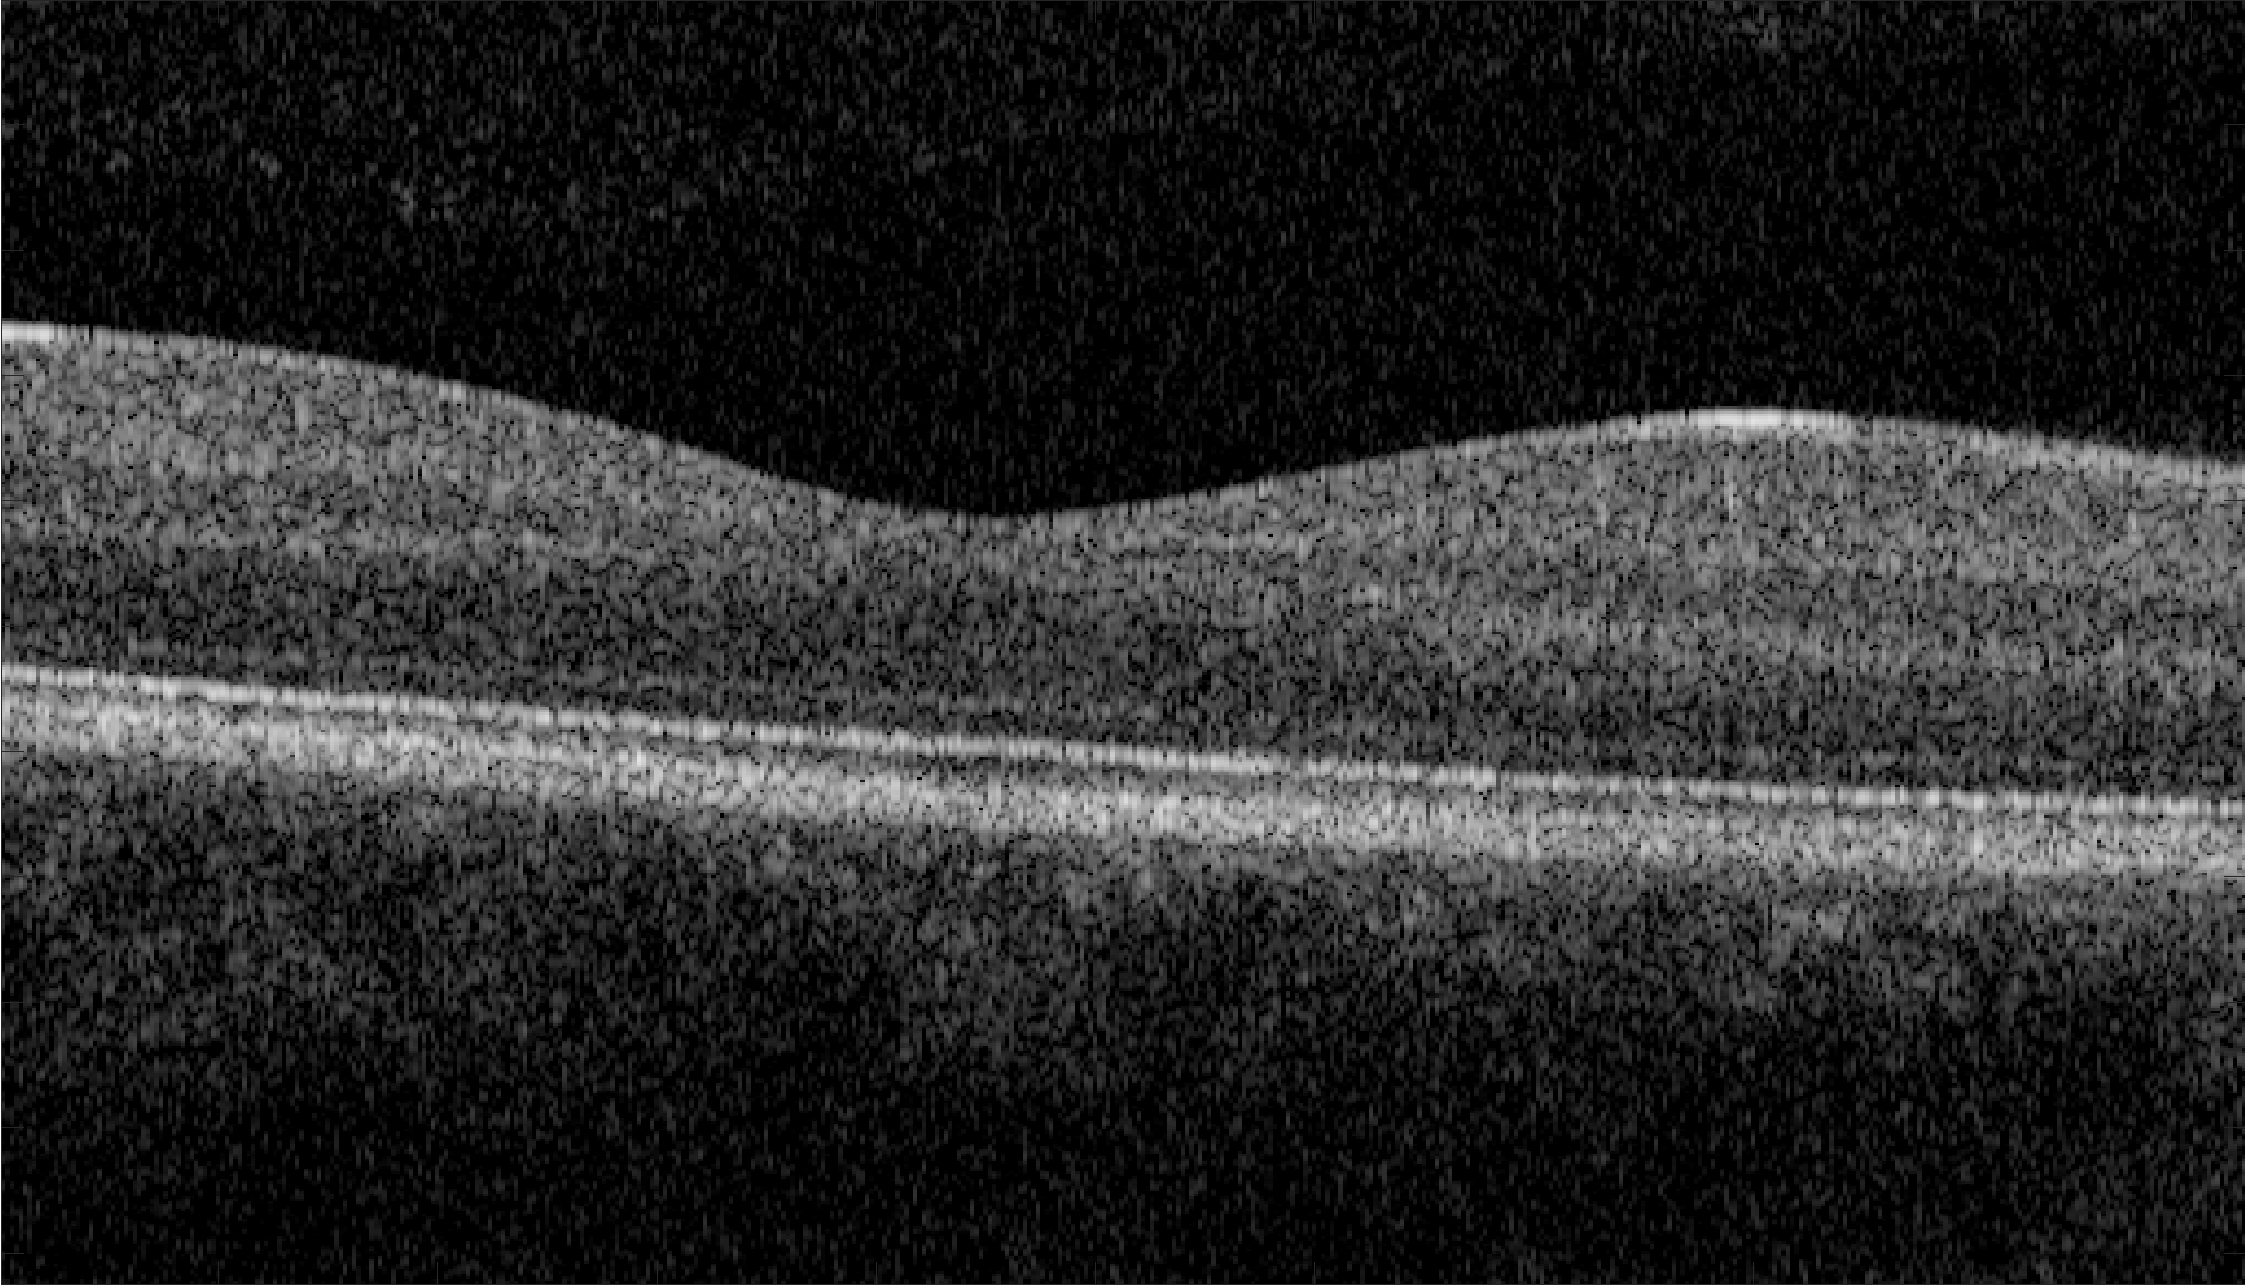
\includegraphics[width=0.7\linewidth]{img/chap3/Retina_Noisy_Bscan}
\caption[Imagen de la retina afectada por ruido de \textit{speckle}]{Imagen de la retina afectada por ruido de \textit{speckle}.}
\label{fig:Retina_Noisy_Bscan}
\end{figure}


%. El tamaño del \speckle en general puede contralarse a través de variaciones en la apertura numérica del sistema óptico, una apertura numérica menor produce patrones de \speckle relativamente grandes, mientras que una apertura numérica grande genera patrones más finos. 

La presencia de \speckle degradador reduce la calidad de las imágenes obtenidas por OCT, y en general, es deseable poder suprimir sus efectos, mientras se conserva la calidad de la imagen. El ruido causado por \speckle sobre una imagen se conoce como \emph{ruido multiplicativo}, y es un problema que se encuentra en múltiples técnicas de imagen coherente, por ejemplo, los radares de apertura sintética. A continuación, se relacionarán una técnica de filtrado proveniente de esta técnica de imagen, y que muestra un alto potencial para eliminar ruido en el caso de OCT.


\section{Del filtrado de \textit{speckle} en SAR a OCT}
\label{sec:from_SAR_to_OCT}

Los radares de apertura sintética (SAR) son una tecnología que ha visto un amplio desarrollo en los últimos años, gracias a las ventajas que posee para producir imágenes de terrenos de varios cientos de kilómetros. Los SAR han sido ampliamente utilizados para el estudio de procesos dinámicos en la superficie de la Tierra, ya que tiene la característica de proveer imágenes con alta resolución (en el orden de $1mm$) que son independientes de la luz solar, la presencia de nubes en la atmósfera e incluso de las condiciones climáticas \cite{Oliver2004,Moreira2013}. Las imágenes SAR son capturadas a través de la medición del eco que se produce en ondas electromagnéticas al ser retroreflejadas por la superficie del terreno analizado. En este caso, las ondas electromagnéticas tienen una longitud de onda que se encuentra del orden de las ondas de radio, con tamaños que abarcan unos cuantos milímetros, lo que permite observar estructuras tales como casas, carreteras, árboles entre otras. Su funcionamiento es análogo al de OCT, por lo tanto, las imágenes son altamente susceptibles al ruido de \textit{speckle} generado principalmente por centros dispersores para la escala de trabajo, siendo estos rocas, hidrantes o estructuras de tamaños similares \cite{Moreira2013}. 

El ruido producido por \speckle degrada altamente las imágenes reconstruidas mediante SAR, y por consiguiente, ha sido un área de gran interés para técnicas de filtrado que preserven estructuras finas mientras se elimina la mayor cantidad de ruido posible, conservando la fidelidad en la imagen filtrada \cite{Novak1990,Lopes2010}. En este sentido, algunas técnicas de filtrado de \speckle han surgido en el contexto de SAR y se han extendido a otras técnicas de imagen coherente, tales como ultrasonido, resonancia magnética y OCT. Sin embargo, pese al desarrollo de esta área, hay múltiples técnicas de filtrado que muestran un alto potencial para su implementación en otras técnicas de imagen coherente y aun están pendientes por explorar.

Inspirados por los resultados obtenidos por Lucas \etal \cite{Lucas2014} en la supresión de ruido por \speckle para los datos provenientes de la luna de Saturno Titan y capturados con la sonda Cassini-Huygens\footnote{Más información en \url{https://saturn.jpl.nasa.gov/mission/spacecraft/huygens-probe/}}, se decidió adaptar ese algoritmo de filtrado a OCT. Titan\footnote{Una imagen con la superficie de Titan filtrada puede encontrarse en \url{http://dralucas.geophysx.org/res.html}} es de alto interés científico por sus características hidrológicas, en donde destacan grandes lagos de metano, montañas de hielo y lluvias de metano en la superficie. Cabe resaltar que a la fecha, todavía se analiza la información enviada por la sonda, y que actualmente la NASA busca investigadores que trabajen con este tipo de datos para ayudar a develar la información hidrográfica que se encuentra en los datos adquiridos. Nuestro objetivo es adaptar el método de filtrado que emplean Lucas \etal para filtrar las imágenes provenientes del Cassini, para usarlo en el filtrado de datos adquiridos mediante OCT, y que de manera similar se encuentran altamente alterados por la presencia de ruido de \textit{speckle}, este algoritmo corresponde a una extensión del \textit{non-local means} (\textit{NL-Means}) mencionado anteriormente. Aunque al inicio de esta investigación, apareció la primera publicación en la cual se emplea \nlmeans en OCT por Yu \etal \cite{Yu2016}, nuestra motivación es poder extender esta técnica para emplear los datos tridimensionales que se adquieren con OCT, y con ello aprovechar mejor los datos disponibles al realizar el posprocesamiento.

%Inspirados por los resultados obtenidos por Lucas \etal \cite{Lucas2014} para la supresión de ruido por \speckle en datos provenientes de la sonda Cassini-Huygens\footnote{Una imagen de Titan filtrada puede encontrarse en \url{http://dralucas.geophysx.org/res.html}} en exploraciones topográficas de Titan, iniciadas en 2005, y cuyo objetivo es develar un mapa de esta luna de Saturno, se decidió emplear el algoritmo de filtrado empleado para las imágenes obtenidas de la sonda Cassini-Huygens. Cabe resaltar que a la fecha, todavía se analiza la información enviada por la sonda, y que actualmente la NASA busca investigadores que trabajen con este tipo de datos para ayudar a develar la información hidrográfica que se encuentra en lo datos enviados desde la sonda. Nuestro objeto es adaptar el método de filtrado que emplean Lucas \etal para filtrar las imágenes provenientes del Cassini, para ser empleado en el filtrado de datos provenientes de OCT, y que de manera similar se encuentran altamente alterados por la presencia de ruido de \speckle. Aunque al inicio de esta investigación, apareció la primera publicación en la cual se emplea \nlmeans para OCT, nuestra motivación es poder extender esta técnica de filtrado para el caso de datos en tres dimensiones, y poder de esta forma aprovechar mejor los datos disponibles en OCT.

\subsection{Principios del \textit{Non-Local Means}}

La técnica de filtrado espacial \nlmeans fue inicialmente propuesta por Baudes \etal \cite{Baudes2005} en el año 2005, \nlmeans aprovecha la redundancia existente en una imagen natural para realizar el filtrado de los datos, esto quiere decir que es posible encontrar una aproximación del ruido y sus características, así como una estimación de la imagen sin ruido empleando unicamente las propiedades intrínsecas de la imagen. En \nlmeans la redundancia de la imagen se aprovecha mediante la comparación de una pequeña zona con sus vecinos, en donde se espera que éstos sigan una forma y estructura definida, así que en lugar emplear unicamente píxeles, se utilizan pequeñas regiones de la imagen. En este contexto, si se tomaran pequeñas ventanas en la imagen, es posible encontrar múltiples zonas similares a lo largo de una región de búsqueda. La Fig.~\ref{fig:lennaPatches} muestra una imagen en donde las zonas indicadas como $\Delta_s$ claramente siguen una distribución espacial similar a las zonas indicadas como $\Delta_{t_1}$ y $\Delta_{t_2}$, con la diferencia de encontrarse a una distancia $\alpha_1$ y $\alpha_2$ de la zona central respectivamente. La región $\Delta_{t_3}$ a una distancia $\alpha_3$ por el contrario, no sigue la distribución de la imagen en $\Delta_s$, pero puede aportar con otro tipo de estadísticas tales como la varianza del ruido.% Empleando esta información y un criterio de similaridad, es posible encontrar la imagen real subyacente en los datos ruidosos.

Para encontrar la información no ruidosa $\nu_s$ en un punto $s$ de un espacio $\Omega$, tal que $s\in \Omega$ y $\Omega$ es del tamaño de la imagen, mediante una estimación $\hat{R}_s$ en base al conjunto de datos ruidosos $R_s$\footnote{Nótese que $\nu_s$ es el conjunto de datos libres de ruido, sin embargo, este conjunto no es posible de obtener, por lo que el filtrado realiza una estimación $\hat{R}_s$ que está directamente relacionada con $\nu_s$.}, \nlmeans emplea una vecindad $\Psi_s$ con $k$ miembros alrededor de un pixel central $s$, tal que una ventana $\Delta_{s}$ centrada en $s$ es comparada con una ventana $\Delta_t$ en todos los puntos $t\in k$ de la vecindad, como se ejemplifica en la Fig.~\ref{fig:patches}. Las ventanas $\Delta_s$ y $\Delta_t$ se denominan ventanas de similaridad, y corresponden a aquellas zonas comparadas, mientras que la vecindad $\Psi_s$ se le denomina ventana de búsqueda y determina la cantidad de vecinos que se compararán. Todas las posibles ventanas en los puntos $t$ se emplean para estimar el valor del pixel $\hat{R}_s$ de la imagen sin ruido. La comparación de un pixel central con sus vecinos, se regula a través de un criterio de \emph{similaridad}, que determina el grado de relación existente entre las zonas comparadas en la ventana de búsqueda.

\begin{figure}[!ht]
	\centering
	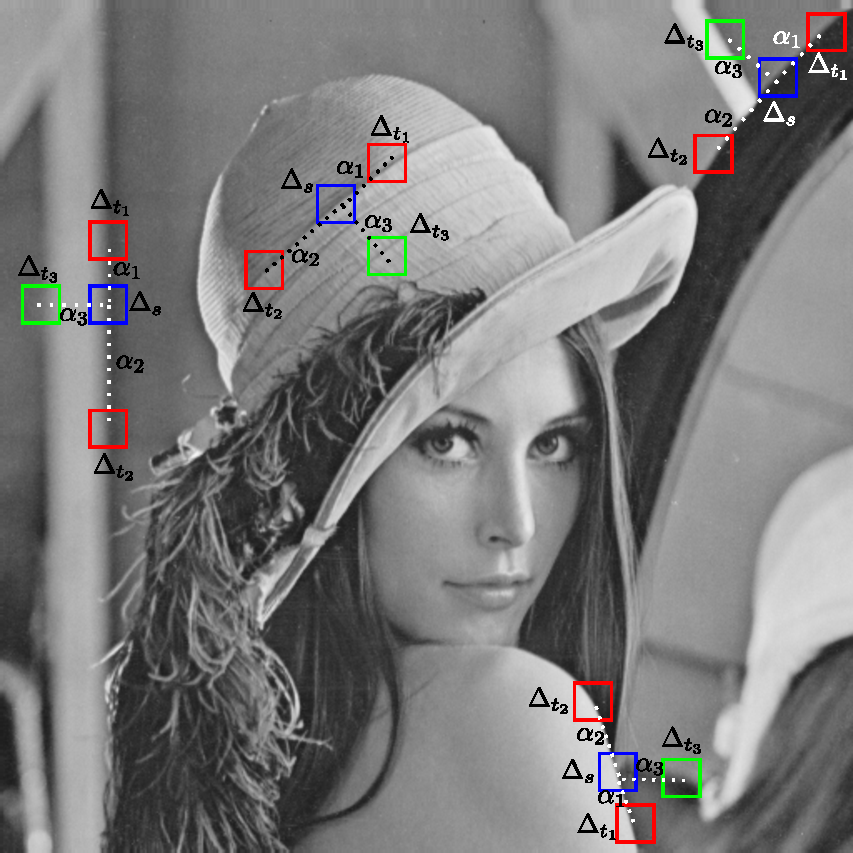
\includegraphics[width=0.5\linewidth]{img/chap3/lennaPatches}
	\caption[Comparación de ventanas en imagen natural.]{Comparación de ventanas en una imagen natural, las ventanas azules centradas siguen la misma distribución de aquellas regiones en rojo, por lo tanto, esta información permite realizar el filtrado de la imagen; este es el concepto en el cual se basa \textit{NL-Means}.}
	\label{fig:lennaPatches}
\end{figure}

\begin{figure}[!ht]
	\centering
	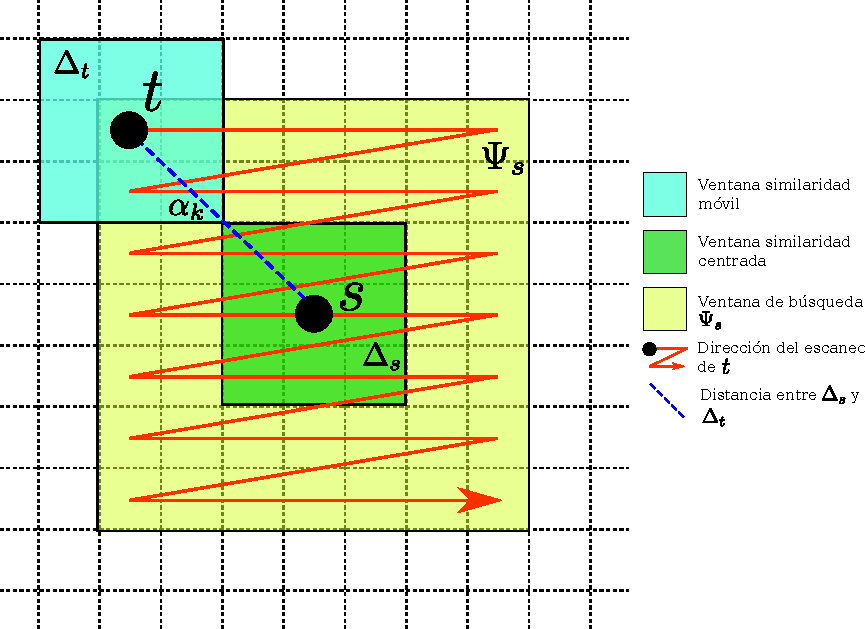
\includegraphics[width=0.5\linewidth]{img/chap3/patches}
	\caption[Dirección de escaneo de \textit{NL-Means}.]{Dirección de escaneo de \textit{NL-Means}, una ventana centradas en $s$ se evalúa con todos los vecinos centrados en $t$, y mediante un criterio de similaridad se realiza el filtrado de la imagen.}
	\label{fig:patches}
\end{figure}

En el contexto del estimador de pesos de máxima probabilidad (WMLE: \textit{weighted-maximum likelihood estimator}) \cite{Baudes2005}, el valor estimado del pixel sin ruido $\hat{R}_s$ se define a partir del conjunto de datos ruidosos $R_t$ como una suma promediada de pesos, esto es

\begin{equation}
\label{eq:R_WMLE}
\hat{R}_s = \frac{\sum_t w(s,t) R_t}{\sum_t w(s,t)},
\end{equation}

\noindent donde $w(s,t)$ corresponde al peso estimado para la ventana de similaridad $\Delta_s$ con respecto a la ventana $\Delta_t$ evaluada en todos los puntos $t\in k$. En la Eq.~\ref{eq:R_WMLE}, el numerador corresponde a la estimación de la similaridad entre las ventanas en la zona de búsqueda, mientras que el denominador es un factor de normalización para que la intensidad total de la imagen no se vea afectada por la suma de pesos. El problema de \nlmeans se encuentra justamente en la definición de los pesos $w(s,t)$, ya que son quienes definen el valor estimado de cada pixel de la imagen. En la propuesta inicial de \textit{NL-Means}, los pesos dependen de un criterio de similaridad entre las zonas a comparar $\Delta_s$ y $\Delta_t$, y se calcula mediante las intensidades en cada una de las regiones; mientras que a su vez dependerá de la distancia $\alpha_k$ que hay entre las zonas $\Delta_s$ y $\Delta_t$, por lo tanto regiones más cercanas tienen un mayor peso que aquellas zonas alejadas de la ventana central. En la Fig.~\ref{fig:lennaPatches} los pesos de las zonas $\Delta_{t_1}$ en general serán mayores que aquellos de las zonas $\Delta_{t_2}$ al encontrarse más cerca de $\Delta_s$, adicionalmente, $\Delta_{t_3}$ debe tener un peso cercano a cero, ya que no sigue la distribución de la imagen en la ventana de similaridad $\Delta_s$.  El hecho de que en este algoritmo, las comparaciones se realicen en una ventana de búsqueda es lo que le otorga la característica no local.

Los pesos $w(s,t)$ se definen \cite{Baudes2005} entonces como
\begin{equation}
\label{eq:nlmeans_normal_w}
w(s,t) = \exp\left(-\frac{1}{h} \sum_k \alpha_k \lvert R_{s,k}-R_{t,k} \rvert^2 \right),
\end{equation}

\noindent donde $\alpha_k$ define un kernel simétrico gaussiano centrado que regula los pesos de acuerdo a la distancia Euclideana que haya entre las zonas $\Delta_s$ y $\Delta_t$ e indica un disminución en la función con respecto a la distancia, $h$ determina el decaimiento de la función exponencial, actuando como un parámetro que regula el nivel de reducción al promediarse las ventanas $\Delta_s$ y $\Delta_t$. $R_{s,k}$ y $R_{s,t}$ son los $k$-ésimos vecinos miembros de las ventanas $\Delta_s$ y $\Delta_t$ respectivamente, éstos corresponden a las mediciones de intensidad experimental que se realizan. 

En general \nlmeans ha mostrado ser un algoritmo robusto para el filtrado de imágenes influenciadas por ruido blanco o ruido gaussiano, y es por ello que ha empleado y mejorado en diversas aplicaciones \cite{Mairal2009,Mahmoudi2005,Kervrann2007,Liu2008,Coupe2008}. Sin embargo, en el caso de ruido por \textit{speckle}, la implementación de \nlmeans no es directa, ya que el criterio de similaridad derivado por Baudes \etal \cite{Baudes2005} fue planteado para el caso de ruido blanco gaussiano. Una extensión de este algoritmo para el filtrado de imágenes provenientes de SAR fue propuesto por Deledalle \etal en 2009 \cite{Deledalle2009} y se conoce como \textit{probabilistic patch-based weights} (PPB), el cual es una extensión de \nlmeans adaptado para filtrar imágenes con ruido de \speckle provenientes de SAR, cuyas características generales difieren en gran medida del ruido blanco gaussiano, y adicionalmente requieren la consideración de diferentes propiedades asociadas con las causas del \textit{speckle}. 

%En el caso de \textit{speckle}, la función de densidad de probabilidad de que un pixel $s$ adquiera una amplitud determinada $A_s$ corresponde a una función del tipo Rayleigh (Sección~\ref{sec:principios_estadistica_speckle}), esta distribución se modifica cuando se promedian múltiples imágenes de una escena, este proceso corresponde al \multilooking, si se promedian $L$ imágenes, la función de densidad de probabilidad de Rayleigh se modifica a una conocida como distribución de Nakagami-Rayleigh, y sigue que

En el caso de \textit{speckle}, la función de densidad de probabilidad de que un pixel $s$ adquiera una amplitud determinada $A_s$ corresponde a una función del tipo Rayleigh (Sección~\ref{sec:principios_estadistica_speckle}). Uno de los procesos más comunes para la reducción de ruido por \textit{speckle}, consiste en el promediado incoherente de múltiples imágenes de la misma escena, esto es promediar varias imágenes de intensidad en un mismo punto, a este proceso se le denomina \textit{multilooking}. El promedio de $L$ imágenes modifica la función de densidad de probabilidad de adquirir una amplitud específica de una distribución de Rayleigh a una conocida como distribución de Nakagami o Nakagami-Rayleigh, que se describe como \cite{Deledalle2009}

%\cite{Coupe2009,Liu2010}
\begin{equation}
\label{eq:p_A_nakagami}
p_A(A) = \frac{2L^L}{\Gamma(L)R_s^L} A^{2L-1}_s \exp\left(-\frac{LA_s^2}{R_s}\right),
\end{equation}

\noindent donde $\Gamma()$ es la función gamma, $L$ se conoce como el número equivalente de vistas (ENL: \textit{equivalent number of looks}), $A_s$ es la amplitud en el campo imagen, y $R_s$ es la intensidad observada de la imagen $R_s = \lvert A_s \rvert^2$. Nótese que en el caso de $L=1$, la Eq.~\ref{eq:p_A_nakagami} es igual a la distribución de Rayleigh mencionada anteriormente, por lo tanto, la Eq.~\ref{eq:p_A_nakagami} es una generalización de la distribución de Rayleigh cuando se realiza \textit{multilooking}. En este contexto, la aproximación de la imagen libre de ruido se realiza también mediante un estimador de pesos de máxima probabilidad similar a la Eq.~\ref{eq:R_WMLE}, de la siguiente manera

\begin{equation}
\hat{R}(s) = \frac{\sum_t w(s,t) A^2(t)}{\sum_t w(s,t)}.
\end{equation}

Deledalle \etal \cite{Deledalle2009} describieron los pesos $w(s,t)$ a través de la combinación de un criterio de similaridad análogo al obtenido por Baudes \etal pero en el caso de ruido causado por \textit{speckle}, añadiendo también, una extensión iterativa al algoritmo. En ésta, se considera la probabilidad de que una zona filtrada $\hat{R}_{s,k}$ corresponda efectivamente a la imagen sin ruido al avanzar las iteraciones del algoritmo. Considerando la extensión del \nlmeans con PPB, y asumiendo que las imágenes se capturan unicamente una vez ($L=1$), los pesos en una iteración $i$ se definen como \cite{Deledalle2009}


\begin{equation}
\label{eq:nlmeans_w}
w(s,t) = \exp \left[-\sum_{k} \left( \frac{1}{h} \log \left(\frac{A_{s,k}}{A_{t,k}} + \frac{A_{t,k}}{A_{s,k}}\right) + \frac{1}{T} \frac{\big\lvert\hat{R}^{i-1}_{s,k} - \hat{R}^{i-1}_{t,k}\big\rvert^2}{\hat{R}^{i-1}_{s,k}\hat{R}^{i-1}_{t,k}} \right)\right].
\end{equation}

Los dos términos que aparecen en la sumatoria de la Eq.~\ref{eq:nlmeans_w} tienen el siguiente significado: $log\left(\frac{A_{s,k}}{A_{t,k}} + \frac{A_{t,k}}{A_{s,k}}\right)$ es el criterio de similaridad obtenido para el caso de ruido por \speckle análogo al mostrado en la Eq.~\ref{eq:nlmeans_normal_w} para el caso de ruido blanco gaussiano; el segundo término $\frac{\big\lvert\hat{R}^{i-1}_{s,k} - \hat{R}^{i-1}_{t,k}\big\rvert^2}{\hat{R}^{i-1}_{s,k}\hat{R}^{i-1}_{t,k}}$ expresa la probabilidad de que las dos zonas filtradas $\hat{R}^{i-1}_{s,k}$ y $\hat{R}^{i-1}_{t,k}$ efectivamente posean las características de la imagen sin ruido luego del filtrado en la iteración $i$, y contribuyen a partir de la segunda iteración para regular el grado de filtrado en las siguientes iteraciones del algoritmo. Estos dos términos se encuentra regidos por los parámetros $h$ y $T$: el parámetro $h$ cumple la función de regular la cantidad de filtrado sobre la imagen, mientras que el parámetro $T$ indica la fidelidad de datos entre iteraciones, esto es qué tan homogénea debe ser la imagen para considerarse como filtrada en la siguiente iteración. Una discusión extendida de los parámetros $h$ y $T$, y su importancia puede consultarse en \cite{Polzehl2006}. En una versión no iterativa del algoritmo, $T\rightarrow\infty$, y la Eq.~\ref{eq:nlmeans_w} corresponde a los pesos solamente dependientes del criterio de similaridad adaptados para el caso de ruido por \textit{speckle}. Finalmente, la Eq.~\ref{eq:nlmeans_w} se considera completamente \textit{no local} ya que no se penaliza de ninguna manera la distancia $\alpha_k$ entre las ventanas de similaridad.

\subsection{Implementación y resultados obtenidos con \textit{Non-Local Means} con PPB}
\label{sec:imple_result_nlmeansPPB}

El algoritmo de la implementación de \nlmeans con PPB se presenta en el Algoritmo~\ref{alg:nlmeansppb}, en donde a partir de la imagen ruidosa, el tamaño de la ventana de búsqueda y de similaridad, la cantidad de iteraciones y los parámetros $h$ y $T$ se calculan los pesos en cada pixel para obtener la imagen filtrada. Una particularidad que tiene \nlmeans se encuentra en la evaluación de los pesos en el pixel central $s=t$, en donde el criterio de similaridad tiende a producir \textit{sobrepeso} comparado con sus vecinos, esto se debe a que las zonas $\Delta_s$ y $\Delta_t$ son iguales cuando $t=s$, y como consecuencia de esto, el criterio de similaridad es máximo. Una opción para corregir este problema, consiste en omitir el pixel central y considerar el peso de éste como el máximo de la ventana de búsqueda, duplicando el mayor de los pesos encontrados, como lo sugiere \cite{Zhang2014}. La última consideración que debe tenerse en la implementación del algoritmo, es que los tamaños de las ventanas siempre deben ser impares para garantizar una región central donde se comparen de manera simétrica las ventanas de similaridad.


\begin{algorithm}
	\begin{tabularx}{0.8\textwidth}{l}
		
		%	\hline
		\textbf{Entrada:} datos ruidosos $R_s$, ventana de búsqueda $W$, ventana\\
		de similaridad $\Delta$, iteraciones $i$, parámetros $h$ y $T$.\\
		\hline
		\hspace*{0.6cm}\textbf{Inicio:} Calcular los pesos correspondientes de cada pixel $s$ en \\
		\hspace*{0.6cm}cada iteración $i$\\
		\hspace*{0.6cm}\textbf{Para} $n = 1 \hspace*{0.2cm} hasta \hspace*{0.2cm} i$\\
		\hspace*{0.9cm} \textbf{Para} $todo \hspace*{0.2cm} punto \hspace*{0.2cm} s$ \textbf{hacer}\\
		\hspace*{1.1cm} Tomar ventana de similaridad $\Delta_s$ de referencia en $s$ con $R_s$\\
		\hspace*{1.1cm} \textbf{luego} calcular vecinos $\Psi_s$ con $W$.\\
		\hspace*{1.1cm} \textbf{Fijar} $w_{max} =w_{tot} = 0$.\\
		\hspace*{1.1cm} \textbf{Para} $t\in \Psi_s$ \textbf{hacer}\\
		\hspace*{1.3cm} Tomar ventana de similaridad $\Delta_t$ \textbf{luego}\\
		\hspace*{1.3cm} calcular peso $w$, con la Eq. \ref{eq:nlmeans_w}.\\
		\hspace*{1.3cm} \textbf{Si} $t = s$\\
		\hspace*{1.5cm} \textbf{Continuar}\\
		\hspace*{1.3cm} \textbf{FinSi}\\
		\hspace*{1.3cm} \textbf{Si} $w > w_{max}$ \textbf{entonces}\\
		\hspace*{1.5cm} \textbf{Fijar} $w_{max} = w$\\
		\hspace*{1.3cm} \textbf{FinSi}\\
		\hspace*{1.3cm} $w_{tot} = w_{tot} + w$\\
		\hspace*{1.1cm} \textbf{FinPara}\\
		\hspace*{1.1cm} Calcular $\hat{R}_s$ con la Eq. \ref{eq:R_WMLE}, $w_{max}$ se duplica.\\
		\hspace*{0.9cm}\textbf{FinPara}\\
		\hspace*{0.9cm} $\hat{R}^{i-1}_s = \hat{R}_s$\\
		\hspace*{0.9cm} $n = n + 1$\\
		\hspace*{0.6cm}\textbf{FinPara}\\
		\hspace*{0.6cm}\textbf{Salida:} Retornar $\hat{R}_s$.\\
		%	\hline	
		
	\end{tabularx}
	\caption{Implementación del \nlmeans con PPB.}
	\label{alg:nlmeansppb}
\end{algorithm}


En la literatura \cite{Deledalle2009,Baudes2005} se recomiendan los siguientes parámetros para el filtrado: las ventanas de similaridad $\Delta_s$ y $\Delta_t$ deben tener un tamaño $\Delta = 7 \times 7$, la ventana de búsqueda $\Psi_s$ un tamaño $W = 21\times 21$, y cuatro iteraciones en el algoritmo $i = 4$. Adicionalmente, una ventaja que tiene la versión iterativa del \textit{NL-Means}, es que permite regular el filtrado de las estructuras finas en las imágenes variando el tamaño de la ventana de búsqueda en la primera iteración \cite{Deledalle2009}, de forma que ventanas más pequeñas tienden a preservar mejor estructuras finas, aunque filtran el ruido en un menor proporción; ventanas más grandes tienden a emborronar regiones de la imagen a cambio de reducir la varianza del ruido y homogeneizar estructuras. %Para los resultados, en la primer iteración, la ventana de búsqueda tuvo un tamaño $W^{(1)} = 7\times7$.
%En una versión no iterativa del algoritmo, $T\rightarrow\infty$ y la Eq.~\ref{eq:nlmeans_w} son los pesos obtenidos para el caso inicial del \textit{NLMeans}, pero adaptados para el caso de ruido de \speckle, adicionalmente, esta extensión se considera completamente no local, ya que no penaliza la distancia que haya entre las ventanas $\Delta_s$ y $\Delta_t$ evaluadas.

Las pruebas experimentales fueron realizadas con un volumen de $512\times512\times256$ [las dimensiones se consideran como $(Z,X,Y)$] con datos tomados en la retina de un paciente, adquiridos con un sistema de OCT comercial, el \textit{Spectralis} de la compañía \textit{Heidelberg Engineering}\footnote{Más información: \url{https://business-lounge.heidelbergengineering.com/int/products/spectralis/}}, los cuales fueron suministrados por el \textit{Wellman Center for Photomedicine}. Sin embargo, para estas pruebas se tomó una sección del volumen de $512\times512$ en $Y=128$ para realizar el filtrado. Es importante mencionar que en OCT la dirección del eje de escaneo rápido corresponde a $X$, mientras que el eje de escaneo lento es $Y$, y al mencionar imágenes se refieren a los datos del plano $ZX$, denominados anteriormente como escaneos tipo B. La imagen que representa los resultados, proviene de la sección transversal de la retina centrada en la fóvea, y muestra una imagen de las capas que la retina posee alrededor de la fóvea, tales como los fotoreceptores en la capa más brillante o los coroides en la capa inferior [Fig.~\ref{subfig:ima_nsy_nlmeansPPB}]. En la Fig.~\ref{fig:ima_filt_nlmeansPPB} se muestra el resultado obtenido para la imagen proveniente del sistema comercial de OCT. La Fig.~\ref{subfig:ima_nsy_nlmeansPPB} corresponde a la imagen ruidosa, la cual se ve fuertemente alterada por la presencia del ruido por \textit{speckle}, de hecho, algunas de las capas menos reflectivas que posee la retina no son diferenciables ya que el ruido degrada la calidad de la imagen, un ejemplo de esto es la región de los coroides, en donde es difícil diferenciar su estructura. La Fig.~\ref{subfig:ima_nsy_nlmeansPPB_multilook} es el promedio de cuatro imágenes con diferentes realizaciones de \speckle de la misma escena, en este caso se aprecia una mejora en la calidad de la imagen debido a que la presencia del ruido se reduce notoriamente, sin embargo, aun se alcanza a percibir ruido ya que este proceso no elimina completamente el \textit{speckle}. La desventaja fundamental de realizar \multilooking es que se debe extender el tiempo de captura de datos en el paciente, lo que deriva en posibles movimiento entre escaneos B, o en algunas aplicaciones de OCT, riesgos para la salud del paciente. La Fig.~\ref{subfig:ima_filt_nlmeansPPB_gaussian} es un filtrado gaussiano de la imagen ruidosa [Fig.~\ref{subfig:ima_nsy_nlmeansPPB}], como en este caso se tiene ruido por \speckle es necesario convertir primero la imagen a escala logarítmica, en donde el ruido por \speckle es aditivo y luego realizar el filtrado, aun así, no hay una mejora sustancial en la calidad de la imagen. Por último, la Fig.~\ref{subfig:ima_filt_nlmeansPPB} es el resultado del proceso de filtrado con los parámetros recomendados por la literatura, y tomando $h = 16$ y $T = 19$, esta imagen presenta alta atenuación del ruido, y permite diferenciar fácilmente las diferentes capas de la retina. No obstante, una inspección detenida de la imagen muestra también algunos problemas respecto al filtrado, por ejemplo el efecto \textit{acuarela} que se percibe, y la presencia de estructuras periódicas finas que aparecen como artefactos.

\begin{figure}[ht!]
	\centering
	\subfigure[Imagen ruidosa.]{\label{subfig:ima_nsy_nlmeansPPB}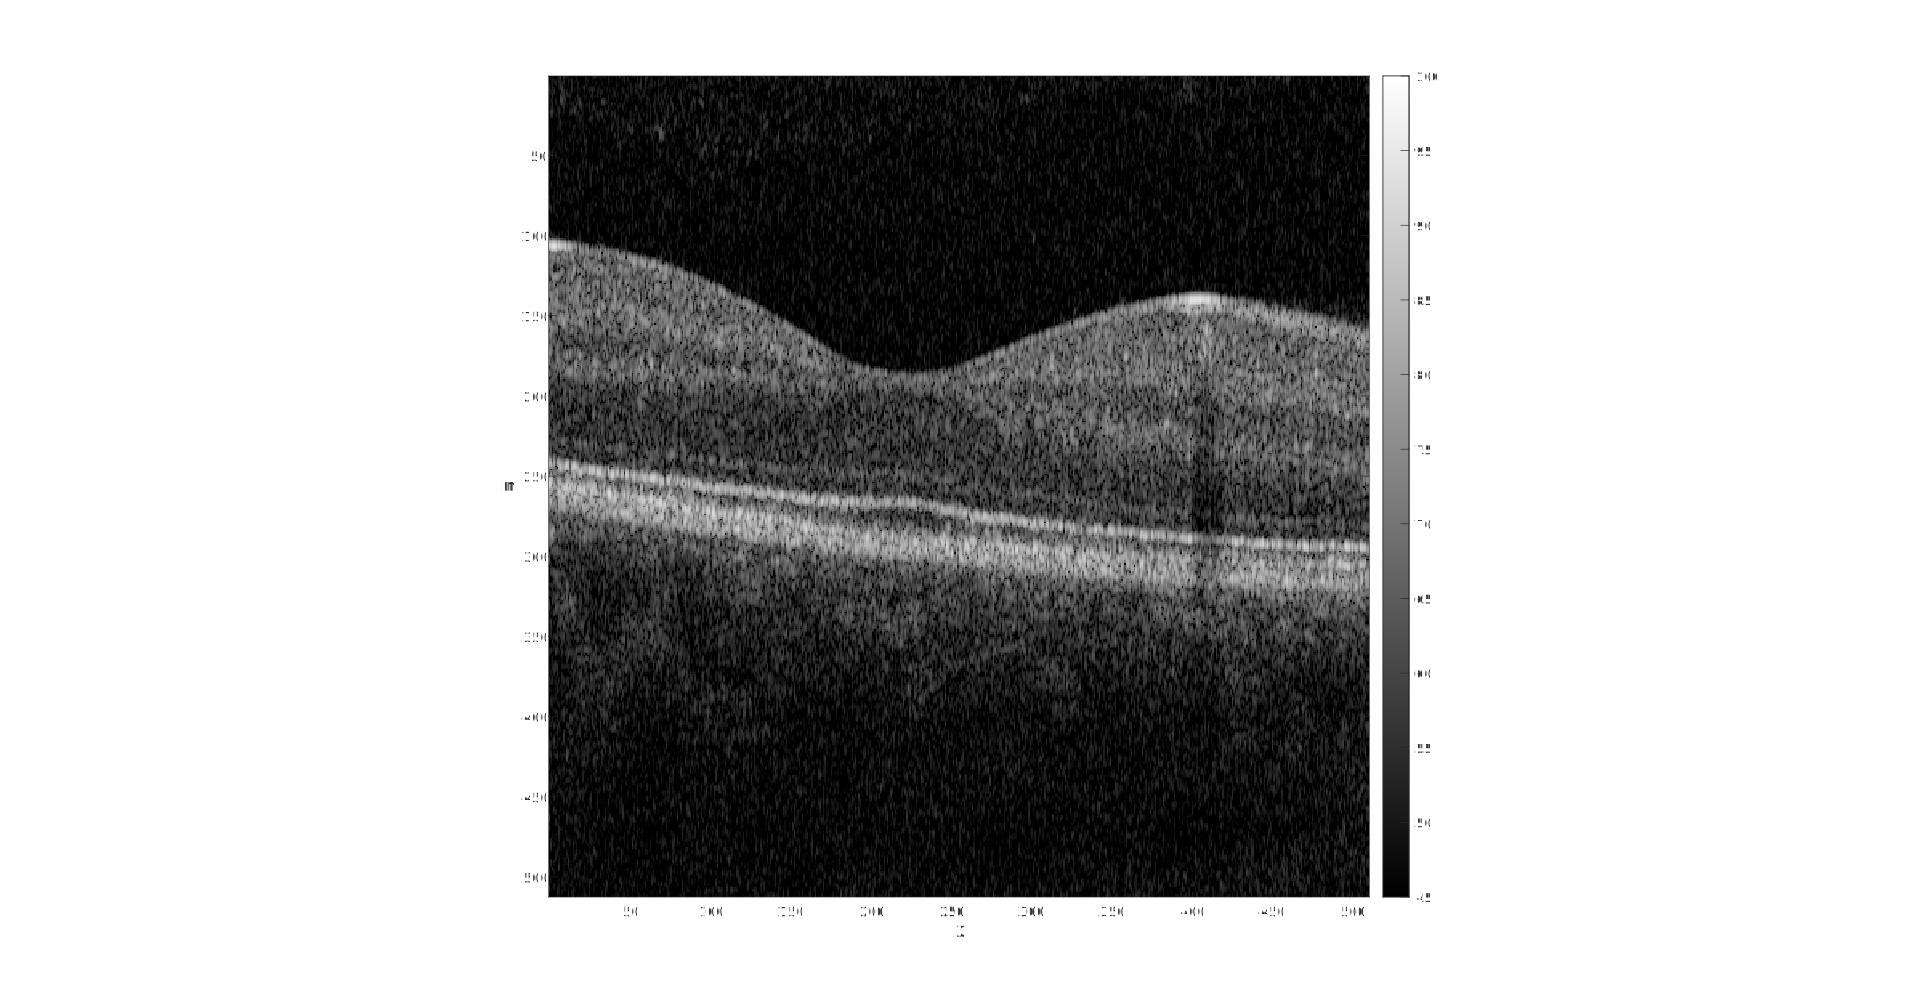
\includegraphics[width=0.4\linewidth]{img/chap3/Retinal_NoisyImage_Bscan128}}
	\subfigure[Imagen resultante del promedio de cuatro imágenes de la misma escena.]{\label{subfig:ima_nsy_nlmeansPPB_multilook}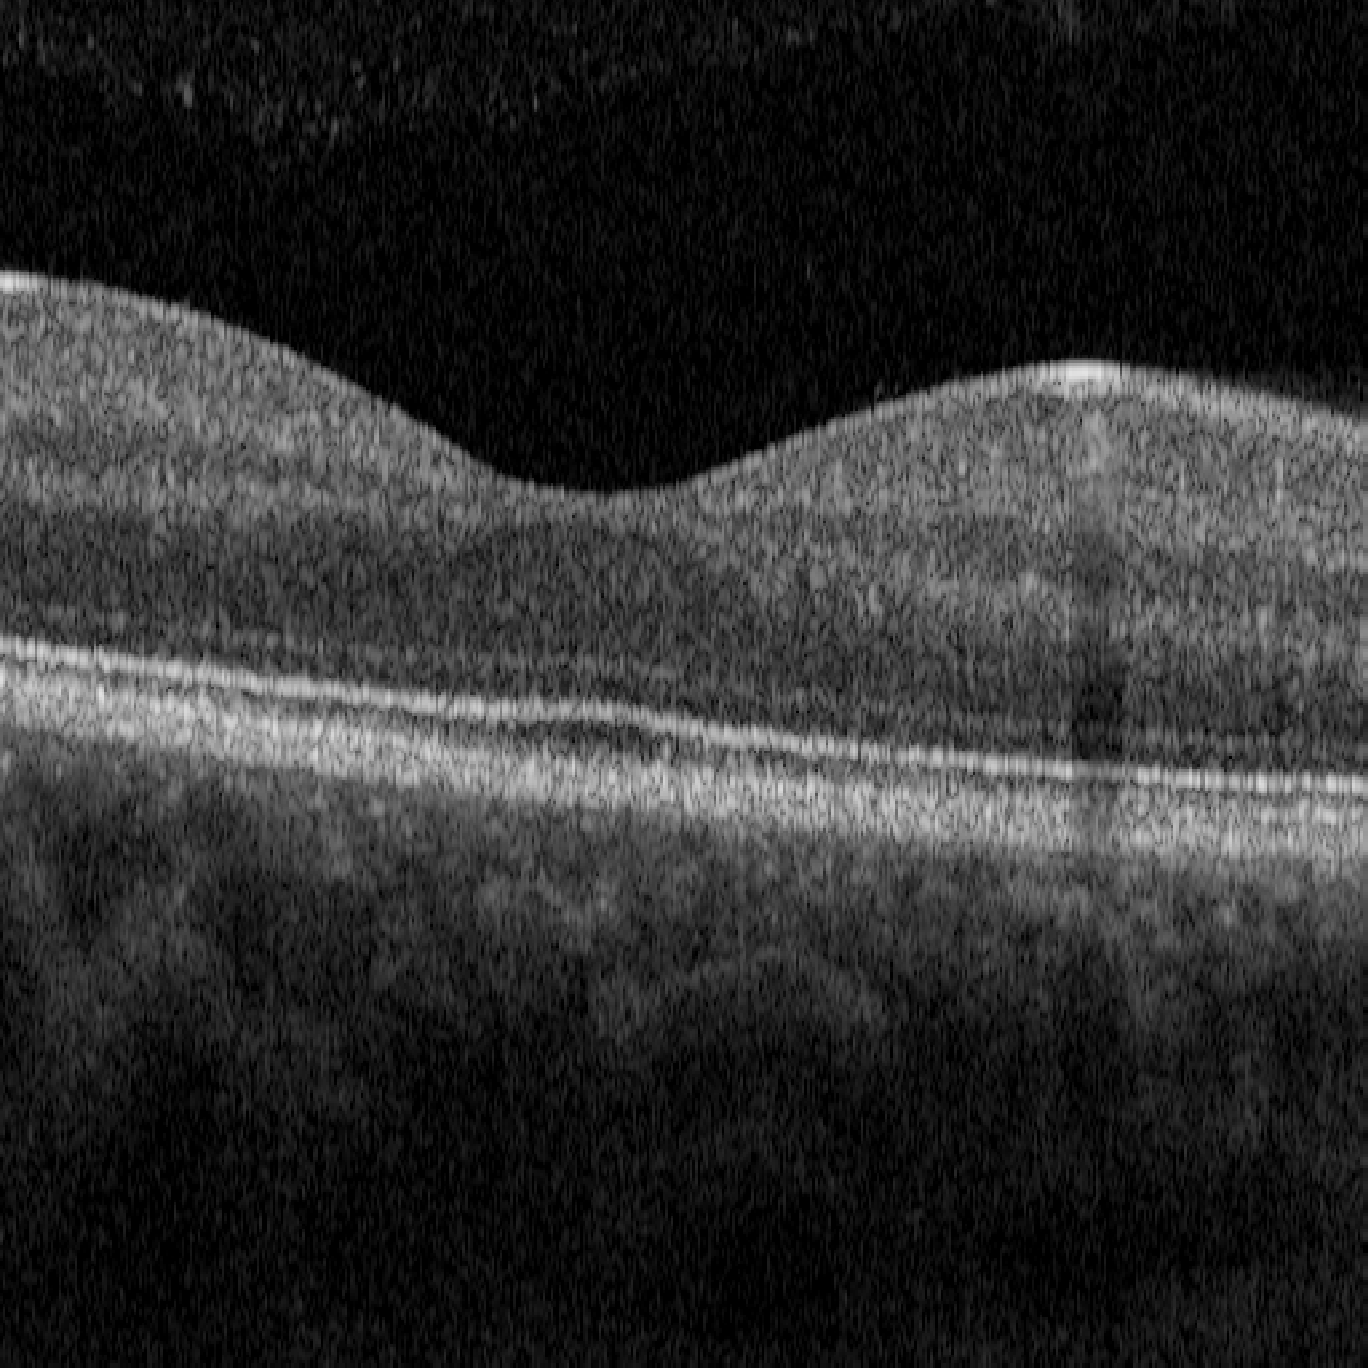
\includegraphics[width=0.4\linewidth]{img/chap3/Retinal_NoisyImage4Mlooks_Bscan128}}
	\subfigure[Imagen filtrada con un filtro gaussiano de tamaño $(7x7)$.]{\label{subfig:ima_filt_nlmeansPPB_gaussian}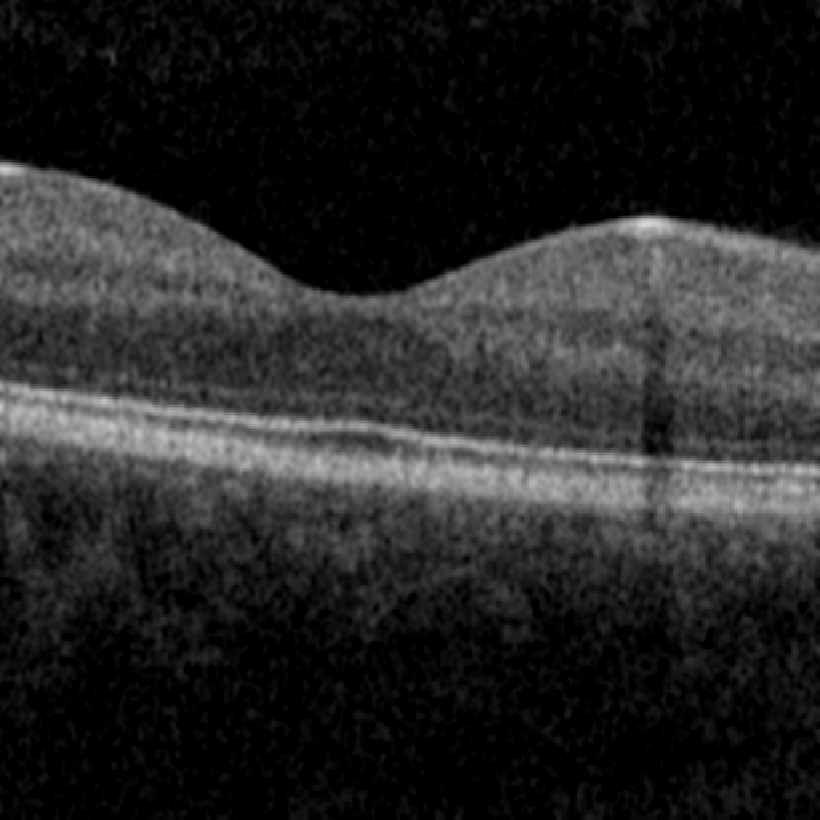
\includegraphics[width=0.4\linewidth]{img/chap3/Retinal_GaussFilter_sigma1d5_Image_Bscan128}}	
	\subfigure[Imagen filtrada mediante \nlmeans con PPB.]{\label{subfig:ima_filt_nlmeansPPB}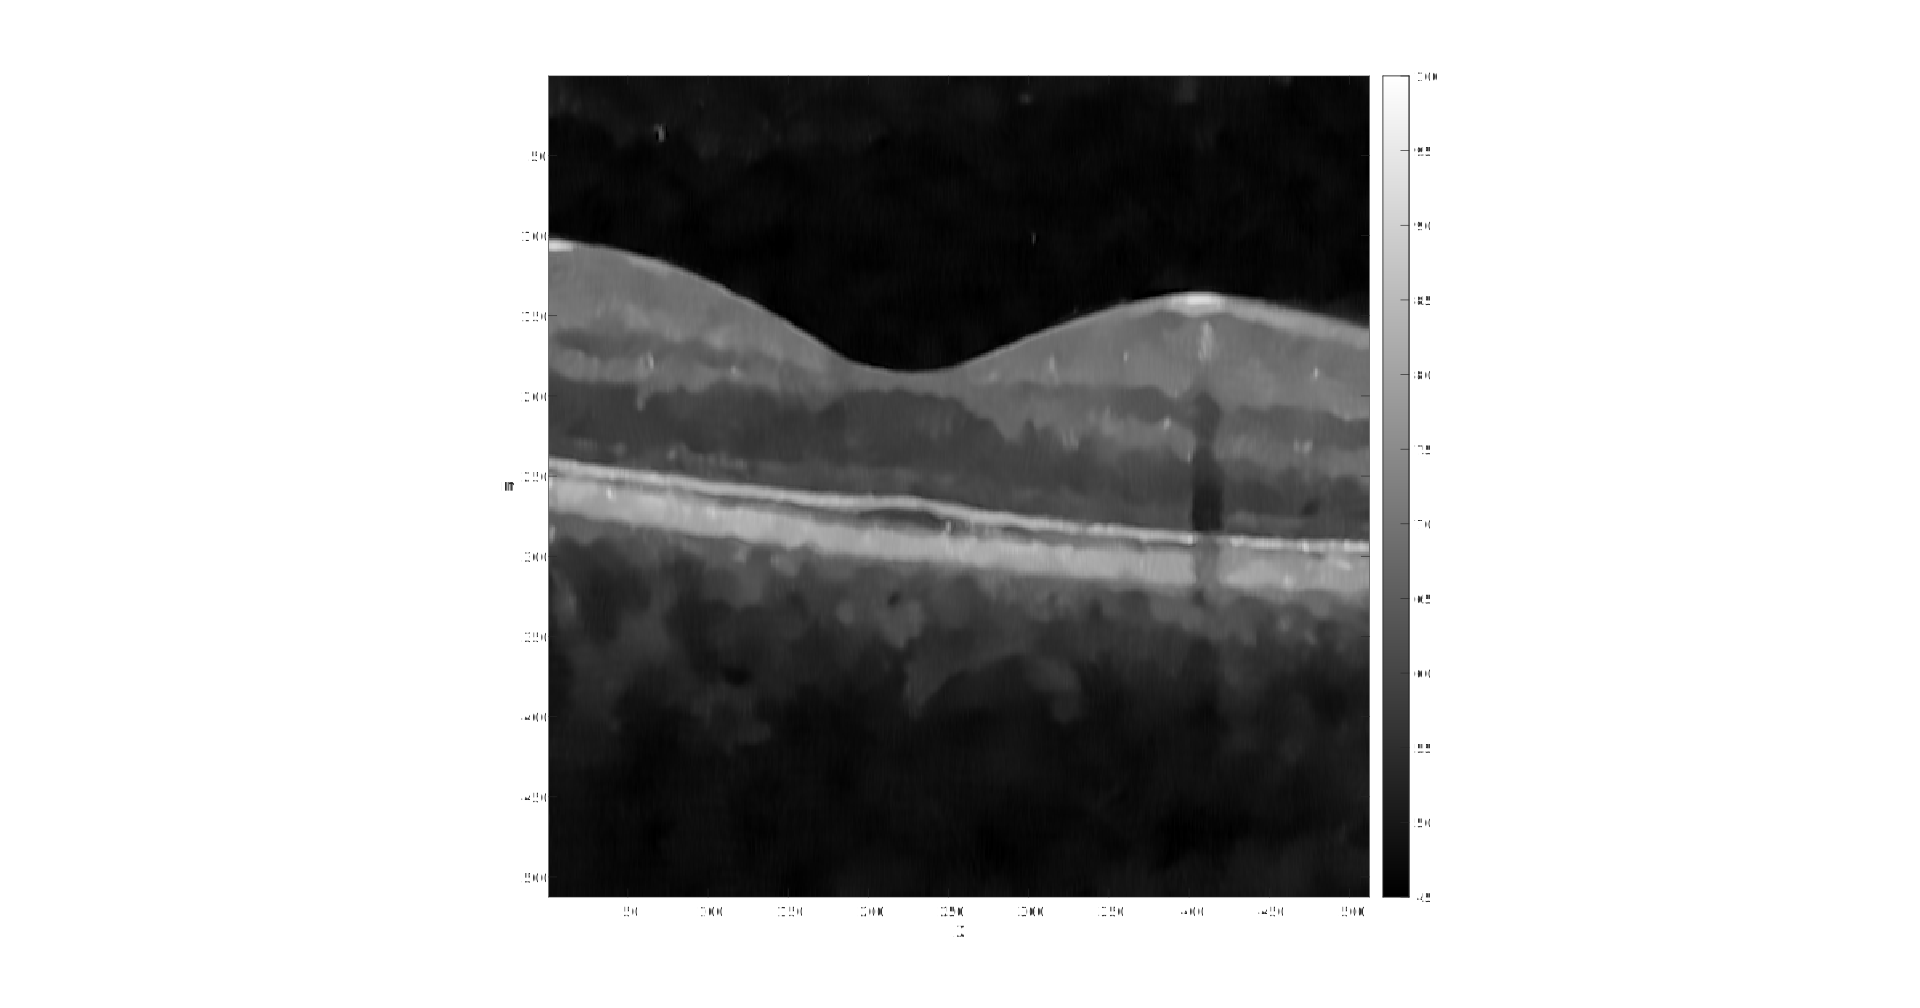
\includegraphics[width=0.4\linewidth]{img/chap3/Retinal_NLMeansIterativo_Bscan128}}
	\caption[Resultado del filtrado de una imagen proveniente de un sistema comercial de OCT para la retina]{Resultado del filtrado de una imagen proveniente de un sistema comercial de OCT para la retina. (a) es la imagen ruidosa capturada donde la presencia del \speckle degrada fuertemente la calidad de la imagen, (b) es el promedio incoherente de cuatro imágenes de la misma región, aunque en este caso hay una mejora en la calidad de la imagen, el ruido por \speckle sigue siendo notorio, (c) resultado del filtro gaussiano de la imagen (a) aunque hay una mejora, la imagen sigue teniendo una alta presencia de ruido, y (d) resultado obtenido con el filtrado mediante \nlmeans con PPB, el ruido por \speckle es altamente atenuado.}
	\label{fig:ima_filt_nlmeansPPB}
\end{figure}

Aunque los resultados de la Fig.~\ref{subfig:ima_filt_nlmeansPPB} muestran que hay una mejora en la calidad de la imagen y que \nlmeans con PPB elimina el ruido indeseado, no es una imagen óptima para ser presentada ante un especialista, quien es el usuario final de los datos luego del filtrado, esto debido a que la imagen pareciera ser sintética y no proveniente de un paciente. Nuestro siguiente objetivo fue mejorar el resultado obtenido con la implementación del \nlmeans con PPB a través de añadir pasos adicionales antes del filtrado. En ese orden de ideas, la primera propuesta que se hizo para mejorar el desempeño del algoritmo, fue la transformación de la imagen proveniente de OCT a una representación diferente, que se conoce como la \textit{representación en coeficiente de atenuación}. La segunda propuesta consistió en obtener y promediar dos imágenes a partir del conjunto de datos, esto es posible a través de la división del espectro medido en dos, y luego tomar sus respectivas transformadas de Fourier. Sin embargo, estas propuestas no mostraron una mejora en el desempeño del filtrado, por lo que se decidió modificar el funcionamiento de las ventanas de similaridad y búsqueda, haciendo uso de la información volumétrica disponible en OCT. En base a esto, se obtuvo que una modificación sobre las ventanas de similaridad y de búsqueda extendidas al caso tridimensional producen un mejor resultado del algoritmo. A continuación se profundizará en las pruebas realizadas y en la propuesta final.

\subsubsection{Representación de imágenes de OCT como coeficientes de atenuación}

La representación en coeficiente de atenuación es una manera alternativa de describir los datos proveniente de un sistema de OCT. El coeficiente de atenuación se puede entender como la reducción de la potencia en un haz que se propaga por un medio turbio, debido al esparcimiento y la absorción que éste experimenta \cite{Vermeer2013}. El coeficiente de atenuación depende de las características del medio, aportando información sobre su composición, es decir, un medio cuyo coeficiente de atenuación sea $5mm^{-1}$ produce un rápido decaimiento de la señal con respecto a la profundidad. La perdida de intensidad de la señal $I(z)$ detectada por el sistema de OCT en función de la profundidad $z$, puede describirse como

%Un medio cuyo coeficiente de atenuación sea grande, produce un rápido decaimiento de la señal con respecto a la profundidad. Como el coeficiente de atenuación depende de las características del medio, aporta información de su composición. 

\begin{equation}
 I(z) \propto e^{-2\mu z},
\end{equation}

\noindent donde $\mu$ es el coeficiente de atenuación y el factor $2$ surge por el viaje de ida y regreso del haz. Siguiendo el tratamiento de Vermeer \etal \cite{Vermeer2013}, una forma alterna de describir la imagen de intensidad de OCT, es a través de la imagen en coeficiente de atenuación, relacionadas de la siguiente manera

\begin{equation}
\label{eq:mu}
\mu (z) = \frac{I(z)}{2\int_{z}^{\infty} I(u)du},
\end{equation}

\noindent es decir, que el coeficiente de atenuación es proporcional a la intensidad registrada en una profundidad con respecto a la intensidad restante en toda la profundidad. Mediante una linearización de primer orden de la función $\log(1+x)$ y considerando la discretización de la imagen de OCT \cite{Vermeer2013}, la Eq.~\ref{eq:mu} puede reescribirse como 

\begin{equation}
\label{eq:mu_i}
\mu [i] \approx \frac{I[i]}{2\Xi \sum_{i+1}^{\infty}I[i]},
\end{equation}

\noindent donde $\Xi$ es el tamaño del pixel e $[i]$ representa los puntos discretos de la imagen. 

La representación en coeficiente de atenuación de la imagen ruidosa en la Fig.~\ref{subfig:ima_nsy_nlmeansPPB} se muestra en la Fig.~\ref{subfig:att_coef_nsy}. Las pruebas realizadas mediante la combinación de filtrado en la representación de coeficiente de atenuación, no mostraron una mejora en el resultado obtenido por medio de \nlmeans con PPB, de hecho, se observó que filtrar la imagen ruidosa en intensidad y luego convertirla a coeficiente de atenuación produce resultados muy similares a filtrar la imagen en términos del coeficiente de atenuación. La explicación de esto se encuentra sustentada en que la transformación integral que se realiza en la Eq.~\ref{eq:mu_i} no modifica la composición del ruido. El resultado del filtrado y posterior conversión a coeficiente de atenuación se presenta en la Fig.~\ref{subfig:att_coef_filt}. Como conclusión, la representación en coeficiente de atenuación no aportó modificaciones relevantes sobre el filtrado del ruido en la imagen, pero permitió ver como el filtrado es invariante ante en la conversión coeficiente de atenuación contra intensidad.

\begin{figure}[ht!]
	\centering
	\subfigure[Imagen ruidosa representada en coeficiente de atenuación.]{\label{subfig:att_coef_nsy}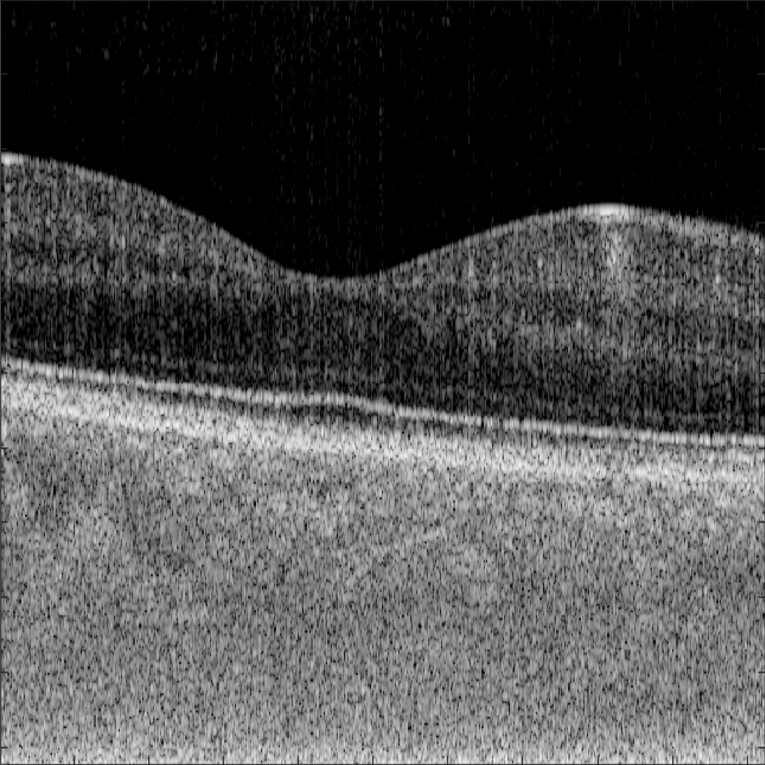
\includegraphics[width=0.4\linewidth]{img/chap3/CoeficientesAtenuacionCorregidos/singlelookAttCoeffNsy}}
	\subfigure[Imagen filtrada representada en coeficiente de atenuación.]{\label{subfig:att_coef_filt}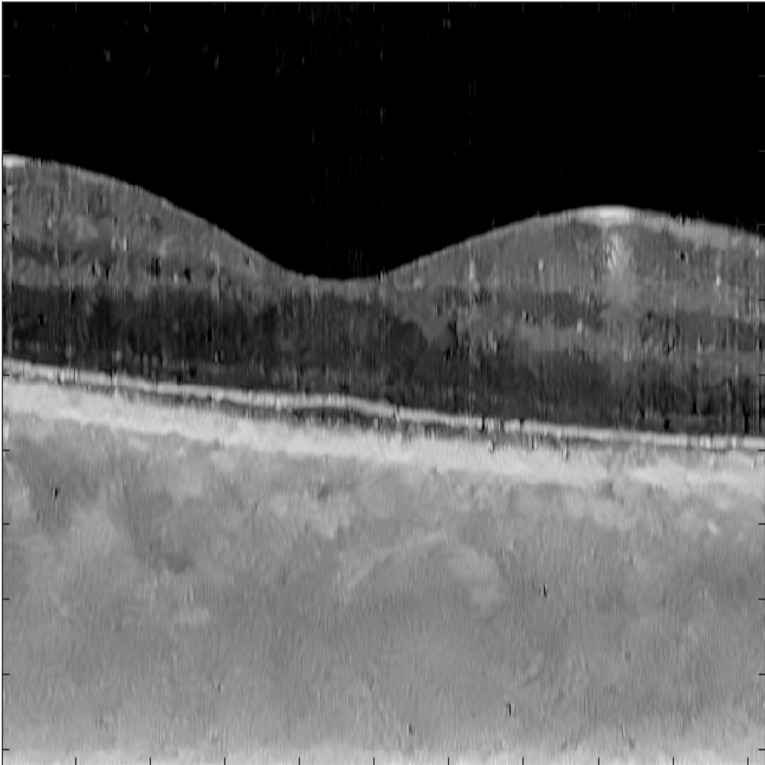
\includegraphics[width=0.4\linewidth]{img/chap3/CoeficientesAtenuacionCorregidos/singlelookAttCoeffFilt}}
	\caption[Representación de imágenes en coeficientes de atenuación]{Representación de las imágenes ruidosa y filtrada en coeficiente de atenuación. (a) imagen ruidosa y (b) imagen filtrada.}
	\label{fig:att_coeff}
\end{figure}

\subsubsection{Obtención de dos imágenes a partir de un solo espectro}

La captura de los datos en sistemas de OCT en el dominio de Fourier como se mencionó en la Sección \ref{sec:int_baja_coh_fourier} se realiza a través del registro del patrón de interferencia en el dominio de las frecuencias, en este sentido, los datos capturados se convierten en imágenes mediante una transformada de Fourier. Debido a que el espectro de la señal contiene la información proveniente de todas las contribuciones, es posible dividir el espectro para obtener múltiples imágenes que contengan una cantidad reducida de información de la escena. Esto quiere decir, que desde un solo espectro pueden derivarse múltiples imágenes cuyas realizaciones de \speckle difieran, a través de la asignación de un ancho de banda diferente para cada una de las nuevas imágenes, sin embargo, este procedimiento tiene la desventaja de producir una pérdida de resolución asociada con la limitación del espectro para cada una de las imágenes. 

Como se muestra en la Fig.~\ref{subfig:dos_espectros_de_uno} a partir del espectro azul, dos nuevos espectros pueden ser derivados (rojo y amarillo), éstos comparten la información del espectro inicial en un ancho de banda diferente, por lo tanto, se tendrán diferentes características en la composición del \speckle de las imágenes derivadas al realizar las transformaciones. Si se toma un promedio de las imágenes derivadas del espectro inicial se reduce la presencia de ruido de \speckle de manera similar al promedio de múltiples imágenes de la misma escena. Este procedimiento puede ser útil, ya que como se mostró anteriormente, realizar un promediado incoherente de la misma imagen reduce significativamente el contraste del \speckle y facilita el filtrado de los datos. 

La Fig.~\ref{subfig:2spectra_mean_image} presenta el promedio de las dos imágenes obtenidas a partir de los espectros rojo y amarillo [Fig.~\ref{subfig:dos_espectros_de_uno}], la línea horizontal que aparece se debe a la presencia de artefactos causados por la pérdida de información en los espectros derivados, asimismo, se aprecia una perdida de los detalles tales como los bordes de la imagen. En la Fig.~\ref{subfig:2spectra_mean_image_filt} se encuentra el resultado de filtrar los nuevos datos, esta imagen no muestra una diferencia significativa con respecto a los filtrados realizados anteriormente, además tiene la desventaja de poseer una menor resolución. Esto permite concluir que intentar generar dos imágenes desde un espectro mediante un intercambio entre resolución y nivel de ruido no es una buena alternativa, ya que no se mejora el desempeño del filtrado y se tiene una reducción en la resolución de la imagen final.


\begin{figure}[h!]
	\centering
	\subfigure[Espectro medido para una línea A.]{\label{subfig:dos_espectros_de_uno}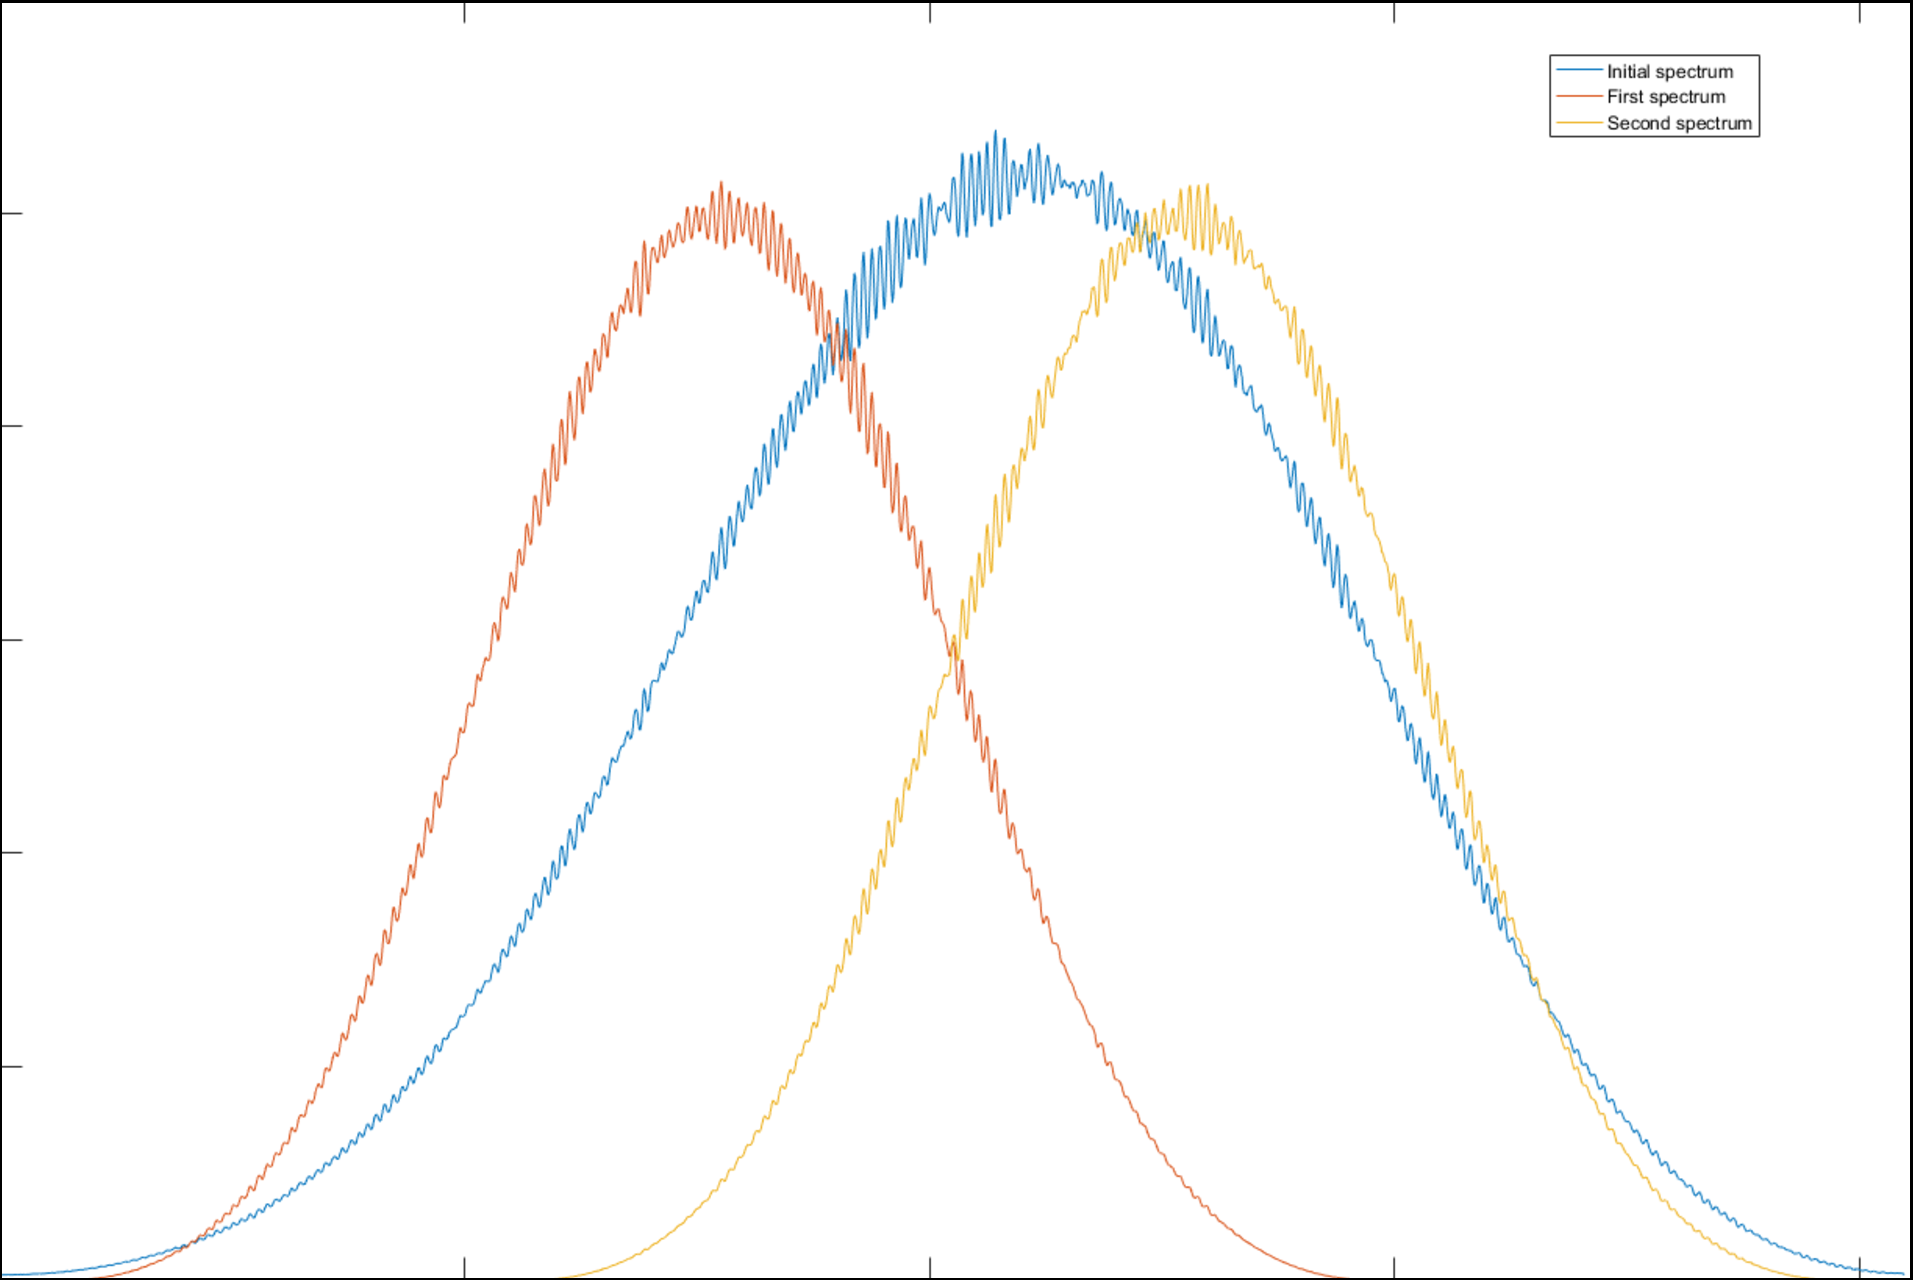
\includegraphics[width=0.4\linewidth]{img/chap3/espectros/EspectrosParticion}}\\
	\subfigure[Imagen obtenida del promedio de las dos subimágenes.]{\label{subfig:2spectra_mean_image}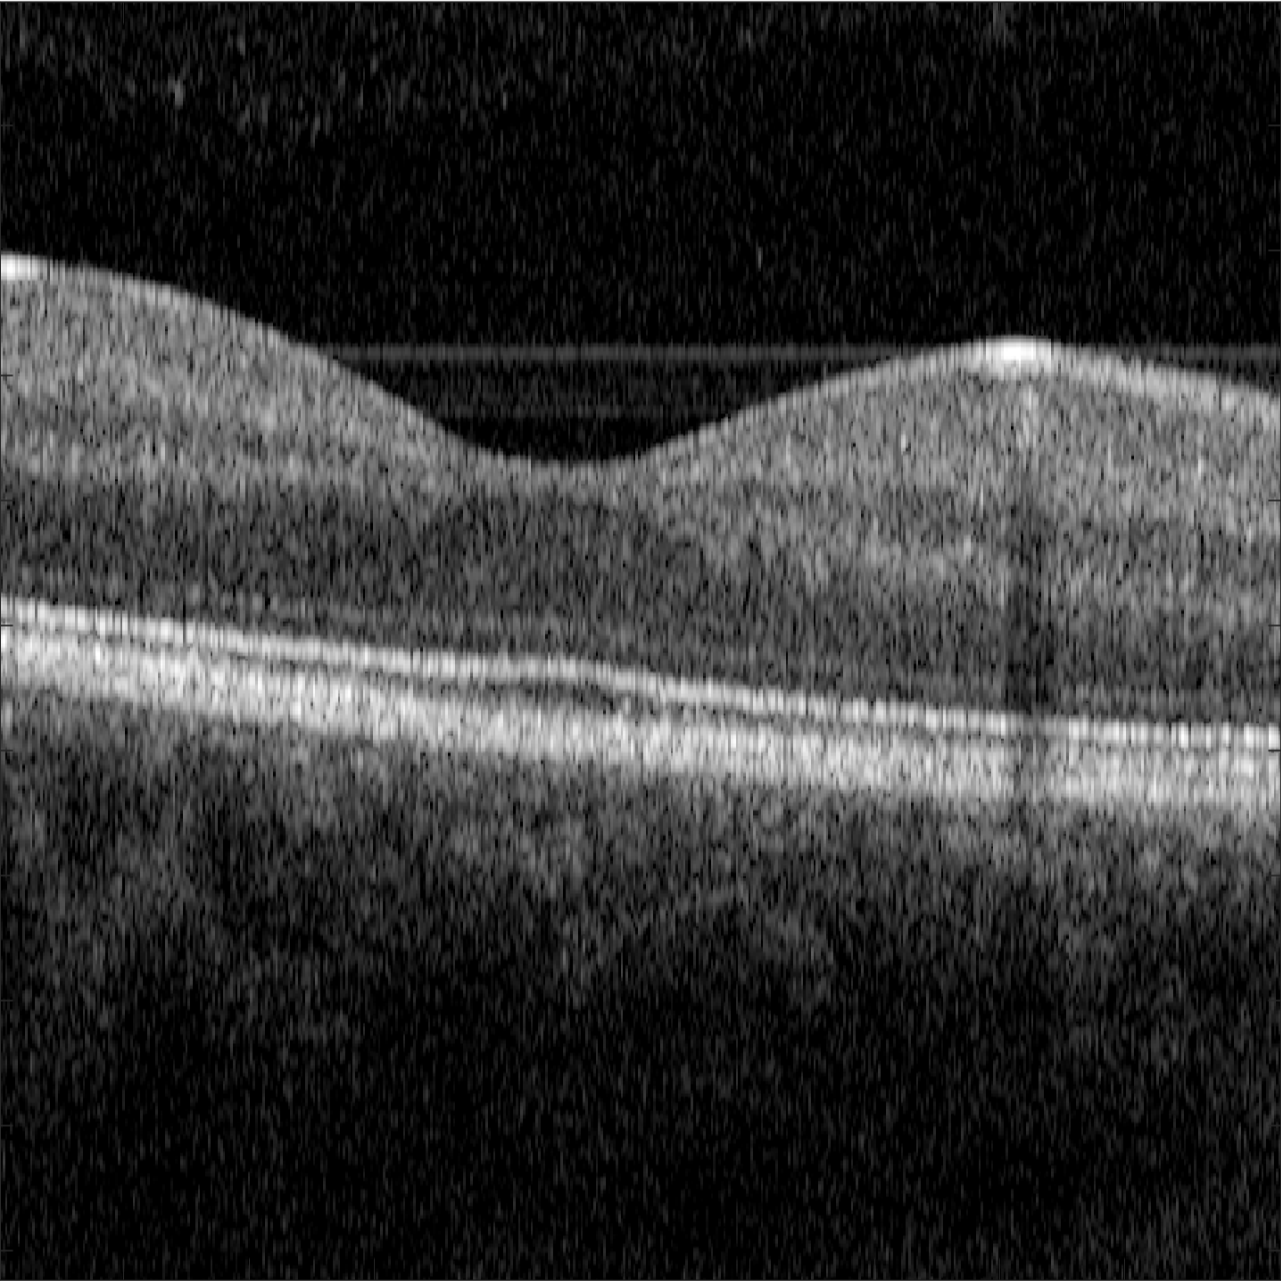
\includegraphics[width=0.4\linewidth]{img/chap3/espectros/imgFrom2SpectraNsy}}
	\subfigure[Imagen proveniente de los dos espectros filtrada.]{\label{subfig:2spectra_mean_image_filt}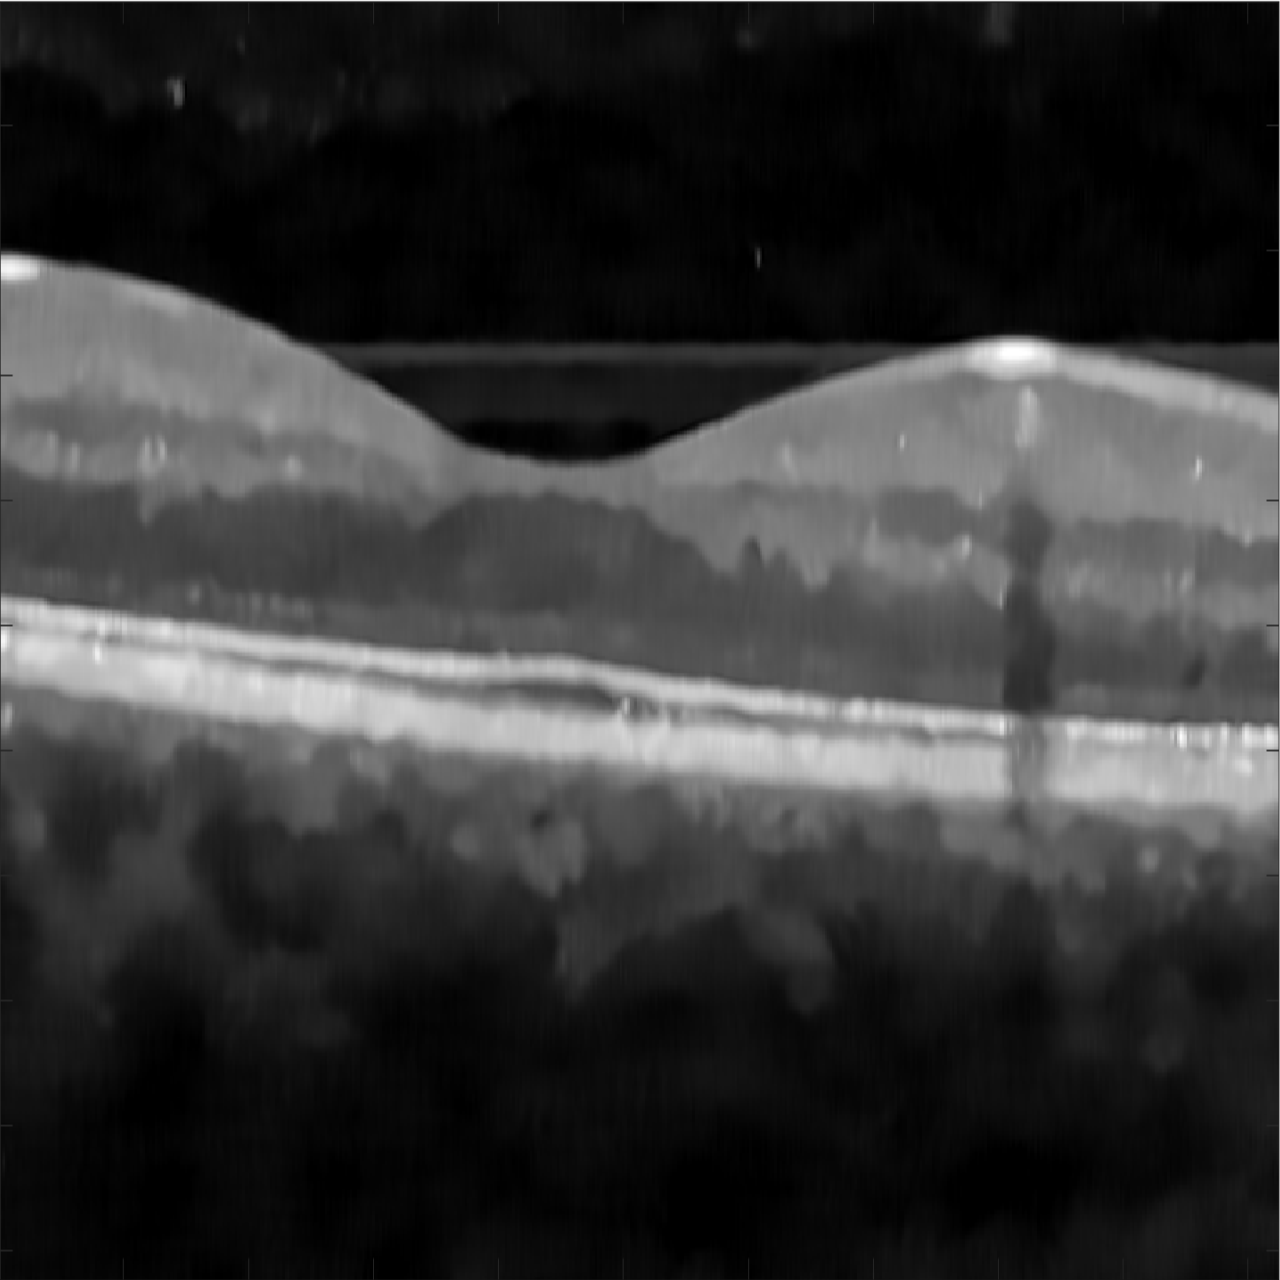
\includegraphics[width=0.4\linewidth]{img/chap3/espectros/imgFrom2SpectraFilt}}
	\caption[Generación de dos imágenes a partir de un espectro]{Obtención de dos imágenes a partir de un único espectro. (a) Los espectros rojo y amarillo se obtiene a partir de espectro azul, en ese caso, se producen dos imágenes con diferentes realizaciones de \textit{speckle} a cambio de una perdida en la resolución axial. (b) imagen ruidosa obtenida del promedio de los espectros amarillo y rojo. (c) imagen filtrada a partir del promedio de dos espectros partiendo de uno.}
	\label{fig:2images_from_one_spectra}
\end{figure}



\subsection{Modificación sobre \nlmeans propuesta (\textit{NL-Means-OCT})}

Las pruebas realizadas añadiendo transformaciones y pasos adicionales al \nlmeans con PPB no mostraron una mejora significativa en los resultados, por lo que luego de realizar múltiples pruebas con variaciones y distintas formas de filtrar, se llegó hasta un resultado que aprovecha y requiere la información volumétrica disponible en OCT. La modificación que se plantea consiste entonces en variar la forma en la que \nlmeans con PPB realiza el cálculo de los pesos entre las ventanas de similaridad al interior de la ventana de búsqueda. Para tal fin, se propone emplear una modificación del \nlmeans en tres dimensiones planteado por Lu \etal \cite{Lu2011} en donde la ventana de búsqueda es cúbica al igual que las ventanas de similaridad, en conjunto con la implementación bidimensional del \textit{NL-Means} con PPB presentada por Deledalle \etal \cite{Deledalle2009}, de la siguiente manera. Partiendo del escaneo propuesto en la Fig.~\ref{fig:patches}, en la cual las ventanas de similaridad $\Delta_s$ y $\Delta_t$, y la ventana de búsqueda $\Psi_s$ son cuadradas, se sugiere modificar las ventanas de similaridad para ser cúbicas, por lo tanto las zonas $\Delta_s$ y $\Delta_t$ adquirirán información sobre los vecinos en las tres dimensiones $(Z,X,Y)$, pero conservando la ventana de búsqueda bidimensional, esto permite filtrar los datos a lo largo de tres posibles planos $ZX$, $ZY$ y $XY$. Los cubos de similaridad $\Delta_s$ y $\Delta_t$ propuestos, así como la ventana de búsqueda $\Psi_s$ se ejemplifican en la Fig.~\ref{fig:Patches_propuesta}.

\begin{figure}
	\centering
	\includegraphics[width=0.4\linewidth]{img/chap3/Patches_propuesta}
	\caption[Modificación de las ventanas de similaridad y búsqueda propuesta.]{Modificación de las ventanas de similaridad y búsqueda propuesta. Las ventanas de similaridad son cubos que toman en cuenta información de sus vecinos, mientras se mantiene la ventana de búsqueda en el plano del eje rápido de escaneo $ZX$.}
	\label{fig:Patches_propuesta}
\end{figure}

%La idea es incrementar la cantidad de datos presente en las ventanas de similaridad, por lo que una mayor cantidad de información se emplea para comparar y por tanto, debe haber una mejora cuando se realiza el filtrado porque se emplean los patrones de \speckle como patrones volumétricos. 

La idea es incrementar la cantidad de datos presente en las ventanas de similaridad ya que son ellas quienes determinan los pesos para el filtro, así se espera una mejora cuando se realiza el filtrado porque se emplean las regiones de la imagen y los patrones de \speckle como volúmenes. La ventana de búsqueda se mantiene bidimensional, ya que si esta tuviese tres dimensiones el tiempo de computo para el algoritmo se vería incrementado en un factor de $\approx 5\times$, además se espera que en esta ventana se encuentre una cantidad suficiente de vecinos para realizar adecuadamente el filtrado, como lo hace \nlmeans con PPB. 

Las posibilidades del plano de orientación de la ventana de búsqueda también tienen una implicación sobre el filtrado, particularmente en el caso de OCT, en donde al tomar los datos experimentales por lo general hay movimientos indeseados que se dan por fuentes externas y producen desplazamientos entre las diferentes imágenes que conforman el volumen; cabe resaltar que éstos desplazamientos se aplican para una imagen entera. En ese orden de ideas, escoger como plano de filtrado aquel correspondiente al eje de escaneo rápido del sistema de OCT ($ZX$), reduce los problemas asociados con movimientos aleatorios causados por el paciente.

En cuanto al cálculo de los pesos también se propone una modificación a la Eq.~\ref{eq:nlmeans_w} utilizada en el \nlmeans con PPB, en este caso, se sugiere emplear una versión no iterativa del algoritmo, es decir, hacer que $T \rightarrow \infty$, y por tanto calcular los pesos $w(s,t)$ de la siguiente manera

\begin{equation}
\label{eq:w_propuesta}
w(s,t) = \exp \left[-\sum_{k} \frac{1}{h} \log \left(\frac{A_{s,k}}{A_{t,k}} + \frac{A_{t,k}}{A_{s,k}}\right) \right].
\end{equation}

\noindent La Eq.~\ref{eq:w_propuesta} es unicamente la adaptación de los pesos para el caso del ruido por \textit{speckle} aplicado a una ventana tridimensional. A esta propuesta se le denominará \textit{NL-Means-OCT}.

\section{Resultados obtenidos y aplicaciones}
\label{sec:resultado_filtrado}

% Con el algoritmo propuesto se realizó nuevamente el filtrado de los datos provenientes del sistema comercial de OCT para la retina, sin embargo, los resultados obtenidos muestran la ventaja del 

\subsection{OCT en la retina}
\label{subsec:oct_retinal}

En el caso de los datos obtenidos para la retina, se empleó el mismo conjunto de datos y un procedimiento similar al planteado en la Sección~\ref{sec:imple_result_nlmeansPPB}, pero tomando en cuenta los cambios propuestos sobre el algoritmo de filtrado, con los siguientes parámetros: tamaño de las ventanas (cubos) de similaridad $\Delta = 7\times7\times7$, tamaño de la ventana de búsqueda $W = 21\times21$ y parámetro de filtrado $h = 18$. A partir de estos criterios se filtró el volumen de $512\times512\times216$ con datos de la retina del paciente, en un computador Intel Core i-7 de $2.93GHz$ (4CPUs) y $6GB$ de memoria, el tiempo de procesamiento total de $69.3$ horas. El resultado obtenido con \nlmeansOCT comparado contra \nlmeans con PPB se presenta en la Fig.~\ref{fig:retinal_ima_nlemans_OCT}. La Fig.~\ref{subfig:retinal_ima_nsy} es igual a la presentada en la Fig.~\ref{subfig:ima_nsy_nlmeansPPB} y corresponde a la imagen afectada por ruido de \textit{speckle}, la Fig.~\ref{subfig:retinal_filtrado_nlmeansPPB} es el resultado obtenido empleando \nlmeans con PPB, la Fig.~\ref{subfig:retinal_filtrado_nlmeansOCT_ZX} representa el resultado obtenido usando \nlmeansOCT con la ventana de búsqueda orientada sobre el plano $ZX$, por último, la Fig.~\ref{subfig:retinal_filtrado_nlmeansOCT_ZY} es la imagen recuperada con \nlmeansOCT ubicando la ventana de búsqueda en el plano $ZY$. 

\begin{figure}[ht!]
	\centering
	\subfigure[Imagen ruidosa.]{\label{subfig:retinal_ima_nsy}\includegraphics[width=0.49\linewidth]{img/chap3/Retinal_NoisyImage_Bscan128}}
	\subfigure[Filtrado con \nlmeans con PPB.]{\label{subfig:retinal_filtrado_nlmeansPPB}\includegraphics[width=0.49\linewidth]{img/chap3/Retinal_NLMeansIterativo_Bscan128}}
	\subfigure[Filtrado propuesto en ZX.]{\label{subfig:retinal_filtrado_nlmeansOCT_ZX}\includegraphics[width=0.49\linewidth]{img/chap3/Retinal/FinalResult_ZX}}
	\subfigure[Filtado propuesto en ZY.]{\label{subfig:retinal_filtrado_nlmeansOCT_ZY}\includegraphics[width=0.49\linewidth]{img/chap3/Retinal/FinalResult_ZY}}
	\caption[Comparaciones del filtrado propuesto]{Comparación de los resultados obtenidos con \textit{NL-Means}, (a) imagen ruidosa, (b) filtrado con \nlmeans con PPB, (c) filtrado propuesto en dirección $ZX$, y (d) filtrado propuesto en dirección $ZY$.}
	\label{fig:retinal_ima_nlemans_OCT}
\end{figure}

La imagen filtrada con \nlmeansOCT mostrada en la Fig.~\ref{subfig:retinal_filtrado_nlmeansOCT_ZX}, ilustra una mejora en algunos de los problemas mencionados anteriormente en el caso del \nlmeans con PPB, en primer lugar, el efecto \textit{acuarela} ocasionado al filtrar la imagen se ha eliminado completamente. Ésto se le atribuye a dos factores principales, al cubo empleado como ventana de similaridad y al uso de la versión no iterativa del algoritmo. Emplear un cubo como ventana de similaridad tiene la ventaja de que las zonas comparadas aportan información volumétrica de las estructuras en la imagen, por ende, es de esperar que las regiones donde hay transiciones entre capas mantengan su suavidad, ya que a diferencia del \nlmeans con PPB, los cambios de capas no son confundidos con bordes en la imagen al momento de filtrar. Asimismo, emplear el cubo de similaridad aporta información sobre los vecinos cercanos, si éstos siguen la misma distribución de la imagen también ayudarán a realizar el filtrado, previniendo el suavizado excesivo de estructuras finas. De la misma manera, el \speckle que se encuentra en las ventanas de similaridad es volumétrico, por lo tanto el algoritmo identifica más fácilmente la presencia de éste en las ventanas comparadas. Otra ventaja que muestra el resultado filtrado es la conservación de puntos brillantes en la imagen, en general, éstos están asociados con características finas en la imagen, tales como la vasculatura. 

La Fig.~\ref{subfig:retinal_filtrado_nlmeansOCT_ZX} se obtuvo al filtrar el volumen de datos sin corregir el movimiento entre las imágenes que conforman el volumen, por ende, hay desplazamientos aleatorios en el conjunto de datos. Los resultados indican entonces que el filtrado propuesto no depende del desplazamiento axial que puedan tener los datos. Este hecho se explica mediante el cálculo de los pesos, en donde al considerar la similaridad entre las ventanas $\Delta_s$ y $\Delta_t$ no hay una dependencia de la distancia entre ellas, sino que se basa unicamente en la evaluación de la similaridad entre las ventanas. Se espera que independiente del movimiento en los datos el algoritmo escoja aquellos vecinos más parecidos, que aportan la mayor cantidad de información al cálculo de pesos independientemente de su posición respecto a la ventana central, y por lo tanto, al ser completamente \emph{no local}, este algoritmo no se ve muy influenciado por desplazamientos aleatorios en el volumen de datos, siempre que la ventana de búsqueda esté ubicada en la dirección del eje rápido de escaneo, generalmente representada como $ZX$. La corrección del movimiento en los datos, debe producir una mejora en los resultados, pero no es un paso necesario para realizar el filtrado, lo cual es ventajoso en aquellas aplicaciones de OCT en donde la corrección del movimiento es complejo, como en OCT gastrointestinal donde las distorsiones causadas por las contracciones musculares tales como la respiración, y los errores instrumentales como la distorsión rotacional no uniforme (NURD) son complejos de corregir \cite{Liang2016, Uribe2015}. 

Para filtrar los datos con la ventana de búsqueda ubicado en el plano $ZY$, fue necesario la corrección del movimiento axial en lo datos, ya que a diferencia de la dirección $ZX$, la continuidad en la ventana de similaridad $\Delta_s$ se pierde y los vecinos en la ventana de búsqueda pierden la relación, reduciendo la similaridad en la ventana de búsqueda. Además, es importante resaltar que si no se corrige los desplazamientos entre imágenes, los datos son difíciles de interpretar en el plano $ZY$. Luego de corregir el movimiento como lo sugiere Kraus \etal \cite{Kraus2012}, se filtró el volumen con la ventana de búsqueda ubicada sobre $ZY$, y a continuación se realizó la proyección de la imagen de interés, el resultado se presenta en la Fig.~\ref{subfig:retinal_filtrado_nlmeansOCT_ZY}. Con respecto a la corrección de movimiento, se observó la presencia de líneas verticales en la imagen, y una mayor diferenciación de las capas, esto está asociado con que el cubo de similaridad ahora posee una estructura definida en las tres direcciones, lo que incrementa el peso de aquellas zonas similares. No se obtuvo una diferencia significativa al realizar la corrección del movimiento y filtrar sobre el plano $ZX$. %En el caso del plano $ZY$ fue posible filtrar,ya que las ventanas de similaridad contenían estructuras comparables, el resultado obtenido de la proyección en $ZX$ del volumen filtrado en el plano $ZY$ se presenta en Fig.~\ref{subfig:retinal_filtrado_nlmeansOCT_ZY}. La diferencia en las transiciones entre capas está directamente asociada a la corrección del movimiento, aun así, este resultado es comparable a filtrar en dirección $ZX$ y no corregir el desplazamiento, lo que se traduce como una reducción de tiempo de procesamiento, y una ventaja en aquellas aplicaciones donde la corrección de desplazamientos aleatorios no es trivial.

Ahora bien, aunque el filtrado en el plano $ZX$ y $ZY$ parece arrojar resultados similares cuando se realiza la corrección del movimiento, hay implicaciones si se quiere realizan proyecciones sobre planos distintos al de filtrado, como lo muestran la Fig.~\ref{subfig:retinal_filtrado_nlmeansOCT_ZX} y la Fig.~\ref{subfig:retinal_filtrado_nlmeansOCT_ZY}. En el caso de las imágenes \enface del volumen, se obtuvo una diferencia para los diferentes filtrados. La Fig.~\ref{fig:retinal_en_face} muestra la proyección \enface del volumen de datos ruidoso y filtrado en diferentes direcciones. En el caso de los datos ruidosos que se presentan en la Fig.~\ref{subfig:en_face_ima_nsy}, la imagen \enface muestra de manera clara la fóvea en la retina acompañada por algunas venas, sin embargo se percibe la presencia del ruido en la imagen. La Fig.~\ref{subfig:en_face_ima_filt_ZX} es la proyección de los datos luego de realizar el filtrado sobre el plano $ZX$, en este caso se da la aparición de unas \emph{líneas} en la dirección $X$ (verticales), que se encuentran relacionadas con la dirección del filtrado. De la misma manera, al filtrar sobre el plano $ZY$, mostrado en la Fig.~\ref{subfig:en_face_ima_filt_ZY} aparecen una \emph{líneas} ubicadas en la dirección $Y$ (horizontales), estas \emph{líneas} se encuentran relacionadas con el plano de orientación de la ventana de búsqueda. La presencia de las \emph{líneas} sobre la proyección en la dirección del filtrado, sugiere que aunque las imágenes no muestren un efecto evidente de filtrar en distintas direcciones, la proyección \enface va a presentar algunos artefactos en esa dirección. La desventaja del algoritmo se encuentra entonces en que no está bien ajustado para permitir proyecciones diferentes al plano en el cual se lleve a cabo el filtrado. Para comprobar esta hipótesis, se realizó un filtrado tridimensional completo, esto es una ventana de búsqueda tridimensional, así como las ventanas de similaridad en tres dimensiones, con tamaños $W=21\times21\times21$ y $\Delta=7\times7\times7$ respectivamente. El resultado del caso 3D se presenta en la Fig.~\ref{subfig:en_face_ima_filt_3D}, nótese como las \emph{líneas} que se presentaban en la dirección de filtrado se eliminan completamente cuando se realiza el filtro completo en 3D, aun así, la desventaja de este, es un incremento en el tiempo de procesamiento de aproximadamente cinco veces con respecto a \textit{NL-Means-OCT}.


\begin{figure}[ht!]
	\centering
	\subfigure[Datos ruidosos.]{\label{subfig:en_face_ima_nsy}\includegraphics[width=0.2\linewidth]{img/chap3/Retinal/EnfaceNoisy}}
	\subfigure[Filtrado en ZX.]{\label{subfig:en_face_ima_filt_ZX}\includegraphics[width=0.2\linewidth]{img/chap3/Retinal/EnfaceZX}}
	\subfigure[Filtrado en ZY.]{\label{subfig:en_face_ima_filt_ZY}\includegraphics[width=0.2\linewidth]{img/chap3/Retinal/EnfaceZY}}
	\subfigure[Filtrado en 3D.]{\label{subfig:en_face_ima_filt_3D}\includegraphics[width=0.2\linewidth]{img/chap3/Retinal/Enface3D}}
	\caption[Comparación proyecciones \enface filtradas]{Comparación de las proyecciones \enface obtenidas con el volumen de datos. (a) proyección \enface con ruido, (b) proyección luego del filtrado en la dirección $ZX$, (c) imagen \enface obtenida al filtrar en dirección $ZY$ en este caso fue necesaria la corrección del movimiento axial entre las imágenes del volumen de datos, y (d) proyección \enface obtenida con el \nlmeans en 3D.}
	\label{fig:retinal_en_face}
\end{figure}

\subsection{OCT en tractografía}
\label{sec:oct_tractography}

En tractografía, uno de los limitantes que tiene la implementación de técnicas ópticas para la reconstrucción de estructuras y tejidos neuronales, se encuentra en la alta atenuación y esparcimiento que experimenta la luz al interaccionar con este tipo de tejidos. Las técnicas de imagen tradicionales empleadas para tractografía, como la resonancia magnética MRI \cite{Basser2000}, tienen la desventaja de poseer una baja resolución en la reconstrucción, es por esto que han surgido técnicas que permiten el análisis del cerebro a partir de otras formas de generación de imágenes. En ese sentido, Chung \etal \cite{Chung2013} propusieron en el año 2013 una técnica de \emph{blanqueado} para tejidos tales como el cerebro, a esta técnica se le denomina {CLARITY}. En \CLARITY se realiza un proceso de infusión del tejido en monómeros formando una mezcla hidrogel-tejido, luego se da una extracción de lípidos mediante un proceso ionizante, las biomoléculas sin grupo funcional se sacan de la mezcla hidrogel-tejido reduciendo las variaciones en el índice de refracción, y por tanto, disminuyendo el esparcimiento y la absorción por parte del tejido. Esto permite que las estructuras se \textit{aclaren}, siendo posible la penetración de luz hasta un rango de $5-6mm$, lo que permite el uso de la microscopía electrónica para el estudio de las características del cerebro, tales como las sinapsis y las densidades postsinápticas. El problema aquí se encuentra en el tiempo de escaneo, ya que este procedimiento puede tardar varios días, y con la degradación de la muestra y los movimientos que esta pueda sufrir el escaneo puede verse alterado. 

Recientemente, Ku \etal \cite{Ku2016} plantearon un procedimiento adicional a \CLARITY que realiza un escalamiento lineal de las estructuras del cerebro, además de producir el efecto de \emph{blanqueado} necesario para su análisis con técnicas ópticas. El procedimiento de reescalado se realiza mediante la adición de acrilamida a la mezcla de hidrogel-tejido junto con un incremento en la temperatura, así se da una expansión lineal en el tejido, siendo este procedimiento reversible mediante la adición de soluciones salinas. Esta expansión lineal permite el uso de otras técnicas de imagen que pueden lograr escaneos más rápidos y mejores resoluciones, logrando analizar con más detalle estructuras finas al interior de tales tejidos. Ku \etal emplearon microscopía en el límite de difracción para obtener imágenes, sin embargo, otras técnicas como OCT pueden lograr escaneos mucho más rápidos, con tiempos de procesamiento del orden de horas, a cambio de una resolución disminuida. La idea es entonces realizar un escaneo mediante OCT del cerebro de un ratón adulto, considerando las limitantes que tiene OCT, como lo son la disminución en la resolución y la presencia de ruido de \textit{speckle}.

Ahora bien, ligado a este procedimiento de reconstrucción del cerebro por medio de OCT, se encuentra también el proceso de tractografía para obtener un mapa de conexiones (\emph{connectome}) del cerebro \cite{Chang2017} a través del análisis de las sinapsis que éste posee. Para realizar el \emph{connectome} es necesario el cálculo de los gradientes en las tres dimensiones con el volumen de datos, luego se escoge la dirección en la que el gradiente sea menor y esto corresponde a la dirección de las conexiones neuronales que realizan las sinapsis. No obstante, el problema que tiene OCT en este tipo de estudio es la presencia de ruido, particularmente el ruido por \speckle que dificulta altamente la obtención del gradiente, y por ende la reconstrucción de las conexiones, hasta ahora, un estudio de este tipo no ha sido realizado. Es, en este punto, donde \nlmeansOCT es altamente relevante, ya que su capacidad para conservar estructuras finas voluméticras, en este caso las sinapsis, y corregir el ruido de \speckle puede aportar en la reconstrucción del \emph{connectome}. 

A partir de esta información, se realizó el filtrado de un volumen de $160\times3600\times128$ con datos provenientes del escaneo del cerebro de un ratón adulto, el tiempo de procesamiento total fue de $35.4$ horas, y se utilizaron los siguientes parámetros de filtrado: ventana de búsqueda $W=17\times17$, ventana de similaridad $\Delta = 7\times7\times7$ y $h=13$. En la Fig.~\ref{fig:brain} se presenta la sección transversal de las sinapsis (puntos brillantes) para el cerebro del ratón. Para realizar el filtrado, es necesario que esas estructuras brillantes se conserven en sus totalidad, ya que son justamente quienes determinan el mapa de conexiones. La imagen de una región de interés de la sección transversal de las sinapsis obtenida con OCT se presenta en la Fig.~\ref{subfig:brain_ima_nsy_zoom}, mientras que el resultado del filtrado con \nlmeansOCT se muestra en la Fig.~\ref{subfig:brain_ima_filt_zoom}. Las sinapsis aparecen entonces como regiones circulares brillantes, con una alta densidad en la región central de la imagen, y se observan algunas más finas, en tanto que otras son más grandes. Nótese cómo la imagen filtrada elimina la presencia del ruido causado por \speckle y conserva en su totalidad las regiones en donde se hallan las sinapsis. En este caso, se optó por un filtrado más suave comparado con el caso de la retina, ya que aquí las estructuras finas tienen una mayor relevancia, es por ellos que se percibe la presencia de patrones periódicos en la imagen, esto está relacionado con el tamaño del \speckle portador de señal, que es el utilizado para formar imagen. La Fig.~\ref{subfig:brain_ima_nsy} muestra la imagen entera de la sección transversal, y la Fig.~\ref{subfig:brain_ima_filt} la correspondiente filtrada, aquí se evidencia mejor cómo el ruido de la imagen se elimina, mientras se conservan las estructuras finas de la imagen.

La proyección \enface de las sinapsis se presenta en la Fig.~\ref{fig:brain_enface}. La Fig.~\ref{subfig:brain_enface_nsy_zoom} es la proyección a una profundidad que permite observar las sinapsis del cerebro en la región de interés, mientras que la Fig.~\ref{subfig:brain_enface_filt_zoom} es la proyección luego de realizar el filtrado. Éstas imágenes permiten observar cómo el filtrado conserva las sinapsis aun cuando éstas se encuentran superpuestas, y se evidencia cómo conservan forma, estructura y dirección. La Fig.~\ref{subfig:brain_enface_nsy} es la proyección \enface completa de los datos del cerebro y la Fig.~\ref{subfig:brain_enface_filt} es la proyección filtrada.

% \cite{Chung2013,Ku2016,Chang2017}.

\begin{figure}[ht!]
	\centering
	\subfigure[Región de interés en la imagen ruidosa.]{\label{subfig:brain_ima_nsy_zoom}\includegraphics[width=0.49\linewidth]{img/chap3/Brain/ima_nsy_short_brain_lines}}
	\subfigure[Región de interés en la imagen filtrada.]{\label{subfig:brain_ima_filt_zoom}\includegraphics[width=0.49\linewidth]{img/chap3/Brain/ima_filt_short_brain_lines}}
	\subfigure[Imagen ruidosa.]{\label{subfig:brain_ima_nsy}\includegraphics[width=1\linewidth]{img/chap3/Brain/ima_Nsy_brain_lines}}
	\subfigure[Imagen filtrada.]{\label{subfig:brain_ima_filt}\includegraphics[width=1\linewidth]{img/chap3/Brain/ima_filt_brain_lines}}
	\caption[Sección transversal del cerebro de ratón]{Imágenes de la sección transversal del escaneo con OCT de un cerebro de ratón.}
	\label{fig:brain}
\end{figure}

Dadas las características de las ventanas de similaridad tridimensionales, \nlmeansOCT permite realizar el filtrado de estructuras finas en los datos que serán empleados para realizar el \emph{connectome} a partir de las sinapsis en el cerebro. Se espera que este resultado facilite el cálculo del gradiente, y por tanto, mejore la precisión del mapa de conexiones generado, asimismo, facilite la implementación de OCT no solo en tractografía, sino que adicionalmente, en la reconstrucción de tejidos a partir de técnicas de expansión y aclarado, mediante la conservación de las estructuras finas en el volumen de datos.

% images inicial
%\begin{figure}[ht!]
%	\centering
%	\subfigure[Espectro de la fuente.]{\label{subfig:2}\includegraphics[width=0.49\linewidth]{img/chap3/Brain/ima_nsy_short_brain_lines}}
%	\subfigure[Espectro de la fuente con filtro.]{\label{subfig:1}\includegraphics[width=0.49\linewidth]{img/chap3/Brain/ima_filt_short_brain_lines}}
%	\caption{Espectros de la fuente halógena de tungsteno, en (a) la resolución axial es de $0.72\mu m$, mientras que en (b) corresponde a $2.14\mu m$.}
%	\label{fig:2}
%\end{figure}
%
%\begin{figure}[ht!]
%	\centering
%	\subfigure[Espectro de la fuente.]{\label{subfig:2}\includegraphics[width=1\linewidth]{img/chap3/Brain/ima_Nsy_brain_lines}}
%	\subfigure[Espectro de la fuente con filtro.]{\label{subfig:1}\includegraphics[width=1\linewidth]{img/chap3/Brain/ima_filt_brain_lines}}
%	\caption{Espectros de la fuente halógena de tungsteno, en (a) la resolución axial es de $0.72\mu m$, mientras que en (b) corresponde a $2.14\mu m$.}
%	\label{fig:2}
%\end{figure}

\begin{figure}[ht!]
	\centering
	\subfigure[Región de la proyección \enface ruidosa.]{\label{subfig:brain_enface_nsy_zoom}\includegraphics[width=0.49\linewidth]{img/chap3/Brain/Enface_zoomed_nsy_lines}}
	\subfigure[Región de la proyección \enface filtrada.]{\label{subfig:brain_enface_filt_zoom}\includegraphics[width=0.49\linewidth]{img/chap3/Brain/Enface_zoomed_filt_lines}}
	\subfigure[Proyección \enface ruidosa.]{\label{subfig:brain_enface_nsy}\includegraphics[width=1\linewidth]{img/chap3/Brain/Enface_nsy_brain_lines}}
	\subfigure[Proyección \enface filtrada.]{\label{subfig:brain_enface_filt}\includegraphics[width=1\linewidth]{img/chap3/Brain/Enface_filt_brain_lines}}
	\caption[Proyecciones \enface del cerebro del ratón]{Proyecciones \enface con los datos del cerebro del ratón.}
	\label{fig:brain_enface}
\end{figure}

\subsection{OCT gastrointestinal}

En el caso de OCT en tractografía se aprovechó el hecho de que \nlmeansOCT preserva estructuras finas por sus ventanas de similaridad cúbicas. En OCT en gastroenterología, el problema que sufren los datos está relacionado con movimientos aleatorios producidos por fuentes externas al sistema óptico, tales como las contracciones musculares durante la respiración, o el palpito del corazón. Esta vez se pretende aprovechar las características \emph{no locales} del algoritmo, particularmente, porque cómo se observó en la retina, no hay una dependencia entre el filtrado y el movimiento aleatorio en los datos. Particularmente en gastroenterología, los desplazamientos que posean los datos son difíciles de corregir, ya que su naturaleza es básicamente aleatoria y no es fácil de modelar matemáticamente. Sin embargo, hay pequeñas causas de movimiento en los datos como la distorsión rotacional no uniforme (NURD: \textit{non-uniform rotational distortion}) \cite{Uribe2015} que se debe a la rotación de la fibra óptica en el catéter, aun así, no todos los problemas pueden ser corregidos.

Ahora bien, otra característica diferenciadora que tiene OCT gastrointestinal, es que la resolución en las tres direcciones puede ser bastante diferente, es decir, que mientras en la dirección $Z$ es típicamente de $\approx 7\mu m$, en $X$ de $\approx15\mu m$ y en $y$ de $\approx50\mu m$. Para poder obtener un filtrado satisfactorio en este tipo de datos, fue necesario modificar \nlmeansOCT para trabajar con ventanas de similaridad y de búsqueda anisotrópicas, de forma que permitiese la selección preferencia de aquellas direcciones en donde la resolución es mayor. Con esto, se filtró un volumen de $732\times4096\times150$ con datos provenientes del esófago de un paciente, en este caso, el tiempo de procesamiento total fue de $124.7$ horas, y se emplearon los siguientes parámetros: tamaño de la ventana de búsqueda $W = 13\times17$, tamaño de los cubos de similaridad $\Delta=7\times9\times5$ y parámetro $h=13$. El tamaño de la ventana de búsqueda se escogió de manera tal que se privilegia la dirección $X$, ya que en esta es la mayor dimensión; el tamaño de la ventana de similaridad, por su parte, fue escogido para dar más peso a las direcciones en donde la resolución es mayor. La selección de estos parámetros podría realizarse mejor si se realizara un algoritmo que determine el tamaño de las ventanas de similaridad en función del tamaño del \speckle volumétrico, esto se propone como trabajo futuro.

El resultado del filtrado de los datos provenientes de OCT gastrointestinal se presenta en la Fig.~\ref{fig:gastrointestinal}. La Fig.~\ref{subfig:GI_ima_nsy_zoom} es una región de interés que permite comparar fácilmente el resultado contra la imagen filtrada en la Fig.~\ref{subfig:GI_ima_filt_zoom}. La Fig.~\ref{subfig:GI_ima_nsy} es un escaneo tipo B del esófago entero, mientras que la Fig.~\ref{subfig:GI_ima_filt} es la correspondiente filtrada. Las imágenes filtradas muestran nuevamente cómo el algoritmo preserva aquellas estructuras de interés, aunque se percibe una particularidad en este tipo de datos en la parte inferior de las imágenes. En estos lugares, la imagen pareciera ser borrosa, esto se debe a que esa región se encuentra por fuera de la zona focal del sistema, y por ende, aparecen como una región desenfocada. Además de esto, la presencia de estructuras periódicas que aparece en la imagen filtrada, se debe al tamaño del \speckle con el cual se forma imagen (\speckle portador de señal). Se concluye entonces, que aun con el movimiento que este tipo de aplicaciones puede experimentar, \nlmeansOCT puede realizar un filtrado que es independiente de los desplazamientos aleatorios que haya entre los datos, ya que finalmente, lo que se busca son aquellas ventanas de similaridad cuya distribución sea similar para realizar el filtrado.


\begin{figure}[ht!]
	\centering
	\subfigure[Imagen ruidosa en una región de interés.]{\label{subfig:GI_ima_nsy_zoom}\includegraphics[width=0.49\linewidth]{img/chap3/GI/ima_nsy_short_GI_lines}}
	\subfigure[Imagen filtrada en un región de interés.]{\label{subfig:GI_ima_filt_zoom}\includegraphics[width=0.49\linewidth]{img/chap3/GI/ima_filt_short_GI_liens}}
	\subfigure[Imagen ruidosa.]{\label{subfig:GI_ima_nsy}\includegraphics[width=1\linewidth]{img/chap3/GI/ima_nsy_GI_lines}}
	\subfigure[Imagen filtrada.]{\label{subfig:GI_ima_filt}\includegraphics[width=1\linewidth]{img/chap3/GI/ima_filt_GI_lines}}
	\caption[Imágenes del esófago filtradas]{Imágenes filtradas en el caso de datos provenientes de un sistema de OCT gastrointestinal.}
	\label{fig:gastrointestinal}
\end{figure}

Las pruebas realizadas con ventanas de búsqueda cuyo tamaño en una dirección era mucho más grande que en la otra, mostraron la presencia de \textit{línea} en la dirección preferencial, esto es \textit{líneas} verticales en el caso de que $Z>>X$, o \textit{líneas} horizontales cuando $X>>Z$, similares a las comparadas en la proyección \enface para los datos de la retina (Sección~\ref{subsec:oct_retinal}).

\bibliographystyle{unsrt}
\bibliography{ref/Ref_chap_3}
\chapter{Estabilización de la fase en OCT}
\label{chapter:estabilizacion_fase}

Uno de los problemas que se puede dar en la adquisición de datos con OCT está relacionado con la falta de sincronía en los sensores y actuadores. Este tipo de problema afecta principalmente la fase, que es importante en aplicaciones que cuantifican flujo mediante OCT. Este capítulo aborda uno de los problemas más comunes en los sistemas de OCT que emplean fuentes de barrido, y propone un método de solución que se basa en la interpretación del problema como una optimización. 

Para esto, el capítulo se divide en cinco secciones en las que se abordarán los siguientes temas: En la Sección~\ref{sec:ofdi} se retomarán los conceptos básicos detrás de OCT con fuente de barrido, en donde uno de los problemas más comunes tiene que ver con la falta de sincronía entre sus componentes, esta dificultad será tratada a fondo en la Sección~\ref{sec:estabilidad_ofdi}. Entendiendo el problema, se planteará una posible solución en la Sección~\ref{sec:propuesta_estabilidad_ofdi}, y describirá el algoritmo, sus principios y las simulaciones en la Sección~\ref{sec:algoritmo_propuesto_ofdi}. Finalmente, se discutirán los primeros resultados experimentales obtenidos con el método propuesto en la Sección~\ref{sec:resultados_experimentales_ofdi}.

\section{OCT con fuente de barrido (OFDI)}
\label{sec:ofdi}

OCT con fuente de barrido (SSOCT: \textit{swept-source optical coherence tomography}), conocido también como imagen óptica en el dominio frecuencial (OFDI: \textit{optical frequency domain imaging}), emplea una fuente de luz sintonizable para producir la interferencia entre el haz de referencia y la luz retroreflejada por la muestra, capturando el patrón de interferencia a través de las componentes espectrales de la fuente, razón por la cual no es necesario desplazar el espejo de referencia. La fuente sintonizable tiene la característica de realizar barridos espectrales con un ancho de banda instantáneo angosto a lo largo de todo el espectro, por lo que se le conoce también como fuente de barrido. El ancho de banda instantáneo corresponde al tamaño de la línea espectral que tiene la fuente mientras se realiza el barrido por las distintas componentes espectrales, de tal modo que la interferencia producida en cada instante del barrido se considera localmente coherente, pues la línea espectral instantánea en general es mucho más pequeña que el espectro total de la fuente \cite{Golubovic1997,Chinn1997,Drexler2015}.

%OCT con fuente de barrido (SSOCT: \textit{swept-source optical coherence tomography}), conocido también como imagen óptica en el dominio frecuencial (OFDI: \textit{optical frequency domain imaging}), emplea una fuente de luz sintonizable para producir la interferencia entre el haz de referencia y la luz retroreflejada por la muestra. La fuente sintonizable, tiene la característica de realizar barridos espectrales con un ancho de banda angosto o instantáneo por todo el espectro, por lo que se le conoce también como fuente de barrido. El ancho de banda instantáneo corresponde al tamaño de la línea espectral que tendrá el ancho de banda mientras se realiza el barrido por las distintas componentes espectrales. La interferencia que se produce en cada instante del barrido se considera coherente, ya que la línea el ancho espectral de la fuente en general es mucho más pequeña que el espectro, y por ende puede considerarse como coherente instantáneamente \cite{Golubovic1997,Chinn1997,Drexler2015}.

%, a este ancho de banda angosto se le denota como ancho de banda , ya que es el tamaño de la línea espectral que la fuente tendrá en algún momento determinado. 

En OFDI no es necesaria la detección con un espectrómetro a diferencia de OCT en el dominio espectral, puesto que las componentes espectrales del patrón de interferencia se encuentran codificadas sobre el barrido, en consecuencia, la señal se captura en un fotodetector como una función dependiente del tiempo sobre el periodo que tarda la fuente en realizar el recorrido por todo el espectro \cite{Drexler2015}. Es necesario entonces relacionar el instante de captura del detector con el número de onda instantáneo emitido por la fuente, la cual se espera que siga una relación lineal con respecto al tiempo \cite{Vakoc2005}. Como el número de onda $k(t)$ del patrón de interferencia registrado por el fotodetector sigue un relación lineal con el tiempo $t$, se puede describir como

\begin{equation}
k(t) = k_0 + \frac{\Delta k}{\Delta t} t,
\end{equation}

\noindent donde $k_0$ es el número de onda inicial del espectro de la fuente, $\Delta k$ es el ancho de banda del número de onda y $\Delta t$ es el periodo de barrido, inversamente proporcional a la frecuencia de la fuente. Al ser el ancho de banda espectral de la fuente finito, la profundidad de penetración máxima $z_{max}$ se encuentra limitada por las características del espectro, siendo esta

%En OFDI, la profundidad máxima de penetración $z_{max}$ se encuentra limitada por el ancho de banda espectral finito de la fuente, siendo en este caso

\begin{equation}
z_{max} = \frac{\lambda_0^2}{4\delta \lambda},
\end{equation}

\noindent donde $\lambda_0$ es la longitud de onda central ($\lambda_0 = 2\pi/k_0$), $\delta \lambda = \Delta\lambda/N_s$ es el intervalo de muestreo de la longitud de onda, $\Delta \lambda$ es la anchura a la mitad del máximo del espectro (FWHM), y $N_s$ es el número de muestras del espectro en $\Delta \lambda$. El intervalo de muestreo  $\delta \lambda$ debe ser más pequeño que el ancho de banda instantáneo de la fuente, ya que de lo contrario, la función de coherencia decaería con la profundidad, limitando el rango de penetración \cite{Drexler2015}.

OFDI es una de las técnicas de captura de datos más comunes para OCT \cite{Leitgeb2003,Choma2003} dado que posee una alta tasa de adquisición, mayor a $50kHz$ por lo que es capaz de producir más de $100$ imágenes por segundo, adicionalmente, tiene una alta sensibilidad del orden de $-120dB$, y una relación señal-ruido baja al capturar todas las profundidades de manera simultánea, viéndose menos afectado por movimientos durante la adquisición. Sin embargo, algunos de los problemas más comunes que se encuentran en OFDI están relacionados con la sincronización requerida entre el sistema de captura de datos y la fuente de barrido \cite{Vakoc2005}, éstos afectan principalmente aquellas aplicaciones en donde la fase juega un papel fundamental, y como se mencionó en la Sección~\ref{sec:plant_problemo}, hay aplicaciones de OCT que dependen altamente de variaciones en la fase, que es donde aparecen los efectos de la baja sincronía y estabilidad de la fase.

\section{Sincronización y estabilidad de fase en OFDI}
\label{sec:estabilidad_ofdi}

Debido a que la adquisición de datos en los sistemas de OCT en el dominio de Fourier se realiza de manera espectral, es necesario realizar transformadas de Fourier para relacionarlos con el dominio espacial. Como las transformadas de Fourier evalúan funciones complejas, los datos en el dominio espacial registrados con OFDI poseen valores complejos, con una amplitud y una fase asociadas. Esta característica permite que algunas aplicaciones de OCT como OCT Doppler cuantifiquen flujo a través del sensado de las variaciones de fase con respecto al tiempo entre líneas A sucesivas, lo cual es posible a través del efecto Doppler que induce el flujo sobre el haz \cite{Zhao2000}. La estabilidad de la fase se convierte entonces en una de las prioridades para aquellas aplicaciones en las que se desea obtener información confiable de cambios que solo pueden medirse a través de la fase. 

El problema de la estabilidad surge a causa de la sintonización que debe hacer la fuente de barrido en el espacio de los números de onda (espacio $k$), en donde no hay un muestreo lineal sobre el espectro, y por ende, se puede dar  una reducción en la resolución espacial del sistema \cite{Brinkmeyer1990}. Una solución para evadir este inconveniente, es que el fotodetector tenga un muestreo con intervalos de tiempo no uniformes, de manera que los datos en el detector se adquieran uniformemente con el muestreo del espacio $k$ durante todo el proceso de toma de datos. Pese a ello, si hay una falta de sincronía entre el detector y la fuente se podrían tener variaciones en la medida de la fase que degradan la sensibilidad de la técnica \cite{Drexler2015}.

La inestabilidad de fase en OFDI puede ser causada también por una variación rápida (\textit{jitter}) en la sincronización entre la fuente y el sistema de adquisición de datos. Este \jitter es un retraso de tiempo aleatorio entre la señal de disparo (\textit{trigger}) y el momento inicial de captura de datos, la incertidumbre en el tiempo de muestreo produce diferencias en el número de onda inicial para cada ciclo de la fuente \cite{Choi2013,Hong2012}. Aunque los retrasos en la señal sean pequeños, hay un impacto importante en la fase del espectro capturado y en la tasa de muestreo, manifestándose en la medida como una diferencia de fase dependiente de la profundidad (una pendiente) en conjunto con un corrimiento aleatorio de fase entre cada una de las líneas A (\textit{offset}) \cite{Liu2015}. Ahora bien, si la fuente de barrido posee componentes mecánicos tiende a tener una estabilidad de fase incluso menor, ya que comparada con una fuente sin parte mecánicas hay más causas de error \cite{Bonesi2014}. En aquellas fuentes donde elementos mecánicos realizan el barrido, el \jitter puede darse por la acumulación de momento que deriva en histéresis y desvíos indeseados, o por inestabilidades en el entorno tales como vibraciones.

Cuando un volumen de datos provenientes de OFDI se encuentre alterado a causa de la falta de sincronía entre el fotodetector y la fuente de barrido, se le denomina tomograma corrupto, ya que hay una corrupción inducida en el mapa de fase medido. Pese a que este problema se encuentra presenta en casi todas las aplicaciones de OFDI, son pocos los algoritmos existentes que permiten mejorar la estabilidad en la fase por medio de métodos numéricos o de posprocesamiento \cite{Adler2007,Vakoc2005,Hong2012,Liu2015}. Nuestro objetivo es proponer una metodología que permita ayudar con la estabilización de la fase en datos obtenidos por medio de OFDI y que presentan una corrupción en la fase por las causas descritas.


%La sincronización del muestreo entre el espacio de los números de onda (\textit{k-space}) donde se asume que la fuente trabaja en un régimen lineal, y el espacio temporal en el cual fotodetector realiza la adquisión de datos 

%\subsection{Phase-resolved optical frequency domain imaging}


\subsection{Características de los tomogramas con corrupción de fase}
\label{sec:caracteristicas_tomogramas_corruptos}

La corrupción en la fase de un tomograma se relaciona con la falta de sincronía entre la señal de disparo de la fuente y el inicio de captura de datos desde el detector. Como consecuencia de esto, hay un corrimiento aleatorio en la fase que no es evidente cuando se trabaja únicamente con la amplitud o la intensidad del tomograma. Si bien los especímenes biológicos analizados con OFDI se caracterizan por tener una fase aleatoria, las mediciones sensibles a la fase requieren de una alta estabilidad durante la captura de los datos. Para ejemplificar el efecto que tiene sobre el tomograma la presencia de corrupción en la fase se realizó una simulación de un volumen de datos con $160\times256\times256$ elementos, siendo las dimensiones respectivas $(Z,X,Y)$. La simulación se basa en el muestreo que realiza un sistema de OFDI y funciona a partir del siguiente esquema:

\begin{itemize}
\item[\textbf{Paso 1:}] Se define un volumen a escanear, tomando en consideración los tamaños físicos y las características de la fuente de barrido.
\item[\textbf{Paso 2:}] Se establece el porcentaje del volumen que estará ocupado por centros dispersores que formarán el \speckle portador de señal y el \speckle degradador de señal, por ejemplo $1\%$ del volumen ocupado por centros dispersores indica una variación en el índice de refracción bajo y por ende, una muestra relativamente homogénea; mientras que un $20\%$ quiere decir que la muestra es altamente inhomogénea.
\item[\textbf{Paso 3:}] Se asignan posiciones aleatorias a cada uno de los centros dispersores del volumen, y a continuación se añaden regiones homogéneas alrededor de algunos de los centros dispersores, formando los objetos a medir.
\item[\textbf{Paso 4:}] Se asigna de una reflectividad superior a aquellos puntos del volumen donde se encuentran los objetos, al haber múltiples centros dispersores se dará la formación de \speckle en todo el volumen, pero en aquellas regiones donde se encuentran los objetos la reflectividad será mayor, haciéndose éstos visibles.
\item[\textbf{Paso 5:}] Se realiza el muestreo del espectro en el espacio $k$, asumiendo que éste es lineal en la señal de OFDI, esto es, generar la función dependiente del tiempo que registra el detector del espacio $k$.
\item[\textbf{Paso 6:}] Para cada una de las líneas A que conforman el volumen, calcular la señal de OFDI producida por los centros dispersores y por el espectro de la fuente, a partir de la señal planteada en la Eq.~\ref{eq:i_D_1}.
\item[\textbf{Paso 7:}] Obtener la transformada de Fourier de cada línea A en el volumen para retornar la señal en el dominio espacial.
\item[\textbf{Paso 8:}] Si se desea añadir elementos de corrupción, adicionar una pendiente y un \offset en la fase de la señal en el dominio espacial, o convolucionar el espectro con una función delta que representa el corrimiento en el número de onda muestreado.
\end{itemize}


En la Fig.~\ref{fig:corruptmap} se presenta una simulación de los datos capturados por un sistema de OFDI. La intensidad del campo simulado se muestra en la Fig.~\ref{subfig:intensidad_clean}, en donde se han ubicado $12$ cilindros, como tener una corrupción en la fase no modifica la amplitud, se espera que independiente de la fase que se imponga no haya una variación en la intensidad medida. En el caso de un sistema de OCT con fuente de barrido, la fase obtenida por medio de transformadas de Fourier representa la fase aleatoria típica de los tejidos, pero con un comportamiento relativamente \textit{suave}, como se presenta en la Fig.~\ref{subfig:fase_limpia}. Sin embargo, cuando hay corrupción a causa de la falta de sincronía, como se ilustra en la Fig.~\ref{subfig:fase_corrupt}, la estructura de la fase [Fig.~\ref{subfig:fase_limpia}] se pierde, y aparecen variaciones aleatorias en la dirección $z$ (verticales) causadas por la dependencia de la fase con la profundidad (pendiente) y su inicio aleatorio (\textit{offset}) entre líneas A.

\begin{figure}[h]
	\centering
	\subfigure[Intensidad.]{\label{subfig:intensidad_clean}\includegraphics[width=0.3\linewidth]{img/chap4/amplitud}}
	\subfigure[Fase normal.]{\label{subfig:fase_limpia}\includegraphics[width=0.33\linewidth]{img/chap4/phase_clean}}
	\subfigure[Fase corrupta.]{\label{subfig:fase_corrupt}\includegraphics[width=0.33\linewidth]{img/chap4/phase_corrupt}}
	\caption[Simulación de volumen de OCT]{Comparación de una imagen simulada de OCT con fase normal y fase corrupta. (a) Intensidad del campo, (b) fase normal y (c) fase corrupta por problemas de sincronización.}
	\label{fig:corruptmap}
\end{figure}

Ahora bien, la corrupción de fase no se hace evidente en las imágenes que se muestran en el dominio espacial, ya que la intensidad no depende de la fase. No obstante, deben presentarse diferencias entre el tomograma normal y el corrupto si se toman transformadas de Fourier, puesto que éstas son sensibles ante la fase del campo complejo. En el caso del tomograma normal, su transformada de Fourier debe seguir teniendo las características del espectro capturado por OFDI antes de realizar imagen, es decir, si no hay corrupción cada línea A que conforma el volumen debe seguir teniendo las propiedades espectrales del haz con el cual se realizó la captura, esto se ilustra en la Fig.~\ref{fig:PSFComparison}. La distribución espectral del tomograma debe entonces continuar siendo una función gaussiana, similar a la que empleó para capturar los espectros que conforman el tomograma, por lo tanto, tomar la transformada de Fourier \enface del tomograma debe producir una función gaussiana reescalada similar a la empleada como iluminación. En todos estos casos se empleó una ventana \text{Hann} o \textit{Hanning} antes de tomar la transformada de Fourier para evitar la aparición de líneas verticales y horizontales por el tamaño finito de la imagen.

%Ahora bien, la corrupción de fase no se hace evidente en las imágenes que se muestran en el dominio espacial, ya que la intensidad no depende de la fase. No obstante, si se toma el campo complejo del volumen de datos y se realizan transformadas de Fourier debido a que la transformada de Fourier es sensible ante la fase, deben presentarse diferencias entre el tomograma limpio y el corrupto. En el caso del tomograma limpio, se espera que su transformada de Fourier siga teniendo las características del espectro capturado por OFDI antes de realizar imagen, es decir, si no hay corrupción, cada línea que conforma el volumen debe seguir teniendo las propiedades espectrales del haz con el cual se realizó la captura, esto se ilustra en la Fig.~\ref{fig:PSFComparison}. La aparición de la distribución espectral de la fuente se debe a que en el dominio de Fourier lo que se capturó fue la convolución entre el objeto y la función de dispersión de punto PSF para el caso de OCT (Sección~\ref{sec:int_baja_coh_fourier}), que se obtiene nuevamente si no hay elementos de corrupción. 

Si el volumen fue capturado bajo las mismas condiciones de iluminación, se espera que cada plano \enface ($XY$) tenga las características de la distribución gaussiana que sigue el haz, como lo muestra la Fig.~\ref{subfig:psf_clean} proveniente de la transformada Fourier de uno de los planos $XY$ del volumen, en donde se observa que el espectro de potencia (PS: \textit{power spectrum}, módulo cuadrado de la transformada de Fourier) del tomograma no corrupto sigue una distribución gaussiana, si se realizaran transformaciones para todos los planos $XY$ en las profundidades todos ellos seguirán esta misma distribución. Por otro lado, cuando hay elementos de corrupción de fase, la distribución que posee el haz en la transformada se pierde dado que hay una alteración aleatoria de la fase, como se puede apreciar en la Fig.~\ref{subfig:psf_corrupt}, en donde la corrupción de fase ha hecho que el PS en $XY$ aparezca como alta frecuencias distribuidas aleatoriamente. 

%Si el volumen fue capturado bajo las mismas condiciones de iluminación, se espera que cada plano \enface ($XY$) tenga las características de la distribución gaussiana que sigue el haz, como lo muestra la Fig.~\ref{subfig:psf_clean} proveniente de la transformada Fourier de uno de los planos $XY$ del volumen, si se realizaran transformaciones para todos los planos $XY$ en las profundidades todos ellos seguirán esta misma distribución. Por otro lado, cuando hay elementos de corrupción de fase la distribución que posee el haz se pierde debido a la dependencia que hay en la transformada con respecto a la fase, como se muestra en la Fig.~\ref{subfig:psf_corrupt}, en donde la corrupción ha hecho que la PSF en $XY$ aparezca como frecuencias aleatorias. 

\begin{figure}[h!]
	\centering
	\subfigure[PS para un plano $XY$.]{\label{subfig:psf_clean}\includegraphics[width=0.19\linewidth]{img/chap4/psf_clean}}
	\subfigure[PS para un plano $XY$ corrupto.]{\label{subfig:psf_corrupt}\includegraphics[width=0.19\linewidth]{img/chap4/psf_clean_pdf}}
	\subfigure[PS para un plano $XY$ con corrupción parcial.]{\label{subfig:psf_patial_corrupt}\includegraphics[width=0.19\linewidth]{img/chap4/psf_partial_corrupt}}
	\subfigure[Promedio de los PS limpias en $XY$.]{\label{subfig:psf_clean_mean}\includegraphics[width=0.19\linewidth]{img/chap4/psf_mean}}
	\subfigure[Promedio de los PS corruptas en $XY$.]{\label{subfig:psf_corrupt_mean}\includegraphics[width=0.19\linewidth]{img/chap4/psf_mean_corrupt}}
	\caption[Espectros de potencia con y sin corrupción]{Comparación de los PS cuando el tomograma está corrupto. (a) PS producido por un solo plano $XY$ limpio, (b) PS obtenido en un solo plano $XY$ corrupto, (c) PS generado por una corrupción parcial en la fase,(d) PS promedio del tomograma limpio, y (e) PS promedio del tomograma corrupto.}
	\label{fig:PSFComparison}
\end{figure}

%\noindent Si el error en la fase causado por el mapa de corrupción es pequeño, hay una pérdida de información al observar la PSF en $XY$, apareciendo como frecuencias altas que no corresponde con la información proveniente de la muestra y que degradan la calidad de la PSF [Fig.~\ref{subfig:psf_patial_corrupt}]. Por último, si no hay corrupción, puesto que todos los planos $XY$ del volumen poseen información sobre la PSF del sistema, si esta se promedia en todos los planos $k$ del espectro se obtiene una distribución similar a la que se empleó para capturar los patrones de interferencia, como se ejemplifica en la Fig.~\ref{subfig:psf_clean_mean}, pero cuando hay corrupción en la fase, esta relación se pierde completamente, y lo que se obtiene esencialmente es una distribución de frecuencias aleatorias al realizar el promedio, como lo muestra la Fig.~\ref{subfig:psf_corrupt_mean}.

\noindent Si el error en la fase causado por el mapa de corrupción está en el orden de los miliradianes, hay una pérdida de información al observar el PS en $XY$, apareciendo como frecuencias altas que no corresponde con la información proveniente de la muestra [Fig.~\ref{subfig:psf_patial_corrupt}]. Por último, si no hay corrupción, puesto que todos los planos $XY$ del volumen poseen información sobre el sistema, el PS promedio de todos ellos obtenido es una distribución similar que muestra un haz gaussiano definido, como se ejemplifica en la Fig.~\ref{subfig:psf_clean_mean}, pero cuando hay corrupción en la fase, esta relación se pierde completamente y lo que se obtiene es una distribución de frecuencias aleatorias al realizar el promedio, como lo presenta la Fig.~\ref{subfig:psf_corrupt_mean}.

La dependencia que hay entre el PS del sistema con respecto a la corrupción de fase debe ser posible de utilizar para caracterizar el mapa de corrupción que ha sido inducido en el volumen de datos. La idea es emplear esta información junto con la modelación que describe el mapa de corrupción en fase para recuperar el tomograma sin corrupción, o equivalentemente el mapa de corrupción, a partir de un algoritmo similar al utilizado en el enfoque de haces coherentes en medios turbios, planteando para ello un problema de optimización.

%Como lo muestra la Fig.~\ref{fig:PSFComparison} hay una alta dependencia entre la PSF en el plano $XY$ respecto al nivel de corrupción. La idea es emplear esta información junto con la modelación que describe un mapa de corrupción en fase, para recuperar el tomograma sin corrupción, o equivalentemente el mapa de corrupción a partir de un algoritmo similar al utilizado en el enfoque de haces coherentes en medios turbios, como un problema de optimización. Esta idea se describirá con más detalle en la próxima sección.

\section{Propuesta para la estabilización de la fase por posprocesamiento}
\label{sec:propuesta_estabilidad_ofdi}

Como se mencionó anteriormente, la propuesta para la estabilización de la fase consiste de dos componentes, por un lado, elementos que se han utilizado en el enfoque de haces coherentes que se propagan a través de medios turbios, y por otra parte, en el planteamiento del problema de la fase como una optimización, conociendo las características del volumen de datos normal y corrupto en OFDI. A continuación, se analizarán y describirán estos dos conceptos.

\subsection{Enfocado de haces coherentes en medios turbios}

En los medios turbios o medios altamente esparsivos y dispersivos, un haz de luz incidente es esparcido a través del medio formando un patrón de \speckle volumétrico que no posee correlación alguna en una distancia mayor a una longitud de onda. El problema se encuentra en que el patrón de \speckle producido por el medio turbio no posee un punto focal medible a la salida del sistema \cite{Vallekoop2007,Cui2011}, no obstante, si se modula el frente de onda del haz antes de ingresar al medio turbio, es posible obtener el patrón de modulación o el cambio de fase necesario para producir un enfoque del haz. Vellekoop \etal \cite{Vallekoop2007} plantearon un método para enfocar un haz que se propaga por un medio turbio, empleando un modulador espacial de luz para inducir un desfase en el haz a la entrada del sistema, y por ende, un enfoque a la salida de éste. El principio de su propuesta es que un haz enfocado produce una intensidad focal 1000 veces más grande que cuando el frente de onda no ha sido modulado. Mediante una optimización simultánea entre el haz enfocado, capturado por una cámara CCD y los niveles de gris en el modulador, los autores fueron capaces de encontrar una fase para cada uno de los 3228 puntos en los cuales se encontraba dividido el modulador, ya que cada uno de ellos producía un punto focal aproximadamente 200 veces más fuerte que el haz no enfocado. La idea de este algoritmo es obtener la fase que produce el mejor enfoque del haz y que corresponde a las variaciones globales que induce el medio turbio a través de medidas de la intensidad luego del enfoque. 

%Considerando que en los medios turbios, cada punto de la fase aporta de manera individual al enfoque del haz, ya que no hay dependencia con respecto a una vecindad del enfoque, cada uno de los elementos del modulador espacial de luz, contribuye de manera individual hasta una intensidad máxima de mejora. El proceso de optimización se basa en que el campo transmitido en la muestra $E_m$, es una combinación lineal de los campos incidentes desde los $N$ segmentos del modulador, de la siguiente manera

Considerando que en los medios turbios cada punto de la fase aporta de manera individual al enfoque del haz ya que no hay dependencia con respecto a un vecino, cada uno de los elementos del modulador espacial de luz contribuye de manera individual hasta una intensidad máxima de mejora. El proceso de optimización se basa entonces en que el campo transmitido en la muestra $E_m$, es una combinación lineal de los campos incidentes desde los $N$ segmentos del modulador, de la siguiente manera

\begin{equation}
\label{eq:e_m}
E_m = \sum_{n=1}^{N} t_{mn}A_ne^{i\phi_n},
\end{equation}

\noindent donde $A_n$ y $\phi_n$ son la amplitud y la fase de luz del segmento $n$. El esparcimiento que experimenta la luz al pasar por la muestra y propagarse por el sistema óptico se describe a través de los elementos $t_{mn}$. Si los términos de $E_m$ en la Eq.~\ref{eq:e_m} se encuentran en fase, entonces, la magnitud del campo transmitido será máxima. La fase de cada segmento, se determina mediante una variación cíclica entre $0$ y $2\pi$ en un proceso iterativo hasta que se obtiene un valor máximo para $E_m$. %En el caso de un medio turbio, las propiedades estadísticas de todos los elementos $t_{mn}$ son independientes. 

La idea de la implementación de este algoritmo al caso de corrupción en fase por inestabilidad en OCT, surge entonces como un análogo al enfoque en medios turbios planteado por Vallekoop \etal \cite{Vallekoop2007}. La propuesta es aplicar los conceptos del enfoque, pero comprendiendo que en el caso de OCT deben haber algunas variaciones en el planteamiento del algoritmo, ya que en lugar de modelar la fase que produce el mejor enfoque, buscaremos aquella pendiente y aquel \offset que aproximan el PS del tomograma corrupto a aquel producido por un sistema sin corrupción, entendiendo este problema como el \textit{enfoque} del tomograma corrupto.%, esta idea se expondrá a fondo en la siguiente sección.

\section{Algoritmo propuesto}
\label{sec:algoritmo_propuesto_ofdi}

%Como se mostró en la Sección~\ref{sec:caracteristicas_tomogramas_corruptos}, si la corrupción en la fase del tomograma es parcial [Fig.~\ref{subfig:psf_patial_corrupt}] la PSF producida por cada plano $XY$, y por consiguiente, la PSF promedio tienden a ser como aquella PSF no corrupta [Fig.~\ref{subfig:psf_clean_mean}]. Sabemos también que el \offset y la pendiente en la fase de cada una de las líneas A del volumen son diferentes, pero es la misma para todos los puntos $z$ de la línea A. En el caso de enfoque en medios turbios, si se encuentra la fase global que introduce el medio en cada uno de los puntos del modulador, se mejora altamente la intensidad de enfoque; en el caso de OCT, cuando el tomograma está corrupto, la PSF promedio que produce pierde completamente la forma gaussiana, sin embargo, si es posible encontrar una combinación pendiente-\offset y aplicar su inversa al tomograma corrupto, debe ser posible recuperar la PSF del sistema que no tiene corrupción. Por lo tanto, partiendo de conocer que cada línea A posee un \offset y una pendiente, y que su tranformada de Fourier no produce la PSF del sistema, tendría que ser factible encontrar esa misma combinación para cada línea A que corrige la corrupción en el tomograma. Bajo este principio e inspirados en la propuesta de Vallekoop \etal \cite{Vallekoop2007}, se propone un algoritmo que evalúa el \offset y la pendiente en cada una de las líneas A que conforman el tomograma, a fin de que por la PSF promedio se recupere el mapa de corrupción que producen una PSF no corrupta.% Para este fin, a continuación se discute el planteamiento del problema.

Como se presentó en la Sección~\ref{sec:caracteristicas_tomogramas_corruptos}, si la corrupción en la fase del tomograma es parcial [Fig.~\ref{subfig:psf_patial_corrupt}] el PS producido por cada plano $XY$, y por consiguiente, el PS promedio tienden a ser como aquel PS cuando el tomograma no está corrupto [Fig.~\ref{subfig:psf_clean_mean}]. Sabemos también que el \offset y la pendiente en la fase de cada una de las líneas A del volumen corrupto son diferentes, pero son las misma para todos los puntos $z$ de la línea A. En el caso de enfoque en medios turbios, si se encuentra la fase global que introduce el medio en cada uno de los puntos del modulador, se mejora altamente la intensidad de enfoque; en el caso de OCT, cuando el tomograma está corrupto, el PS promedio que produce pierde completamente la forma gaussiana, sin embargo, si es posible encontrar una combinación pendiente-\offset y aplicar su inversa al tomograma corrupto, debe ser viable recuperar el PS del tomograma que no tiene corrupción. Por lo tanto, partiendo de conocer que las líneas A con un \offset y una pendiente producen un PS con altas frecuencias aleatorias, tendría que ser factible encontrar la combinación correspondiente para cada línea A que produce el PS correcto. Bajo este principio e inspirados en la propuesta de Vallekoop \etal \cite{Vallekoop2007}, se propone un algoritmo que evalúa el \offset y la pendiente en cada una de las líneas A que conforman el tomograma corrupto, a fin de que a través del PS promedio se recupere el mapa de corrupción.% Para este fin, a continuación se discute el planteamiento del problema.

Durante la adquisición de datos de un tomograma a través de OFDI, se realiza la medición de un conjunto de $N$ espectros $S_n(k)$ que se encuentran corruptos por la falta de sincronización entre el \textit{trigger} de la fuente y el sistema de adquisición de datos. El índice $n$ denota la línea A correspondiente capturada, por lo tanto, $S_1(k)$ será el primer espectro que es la referencia global para los espectros siguientes $S_2(k), S_3(k), \ldots, S_N(k)$, además, cada línea A tiene un muestreo de $M$ puntos. En este orden de ideas, se puede relacionar a $M$ y $N$ con la cantidad de puntos o muestras en la dirección $z$ y en las direcciones laterales $xy$ respectivamente. Para obtener el tomograma en el dominio espacial, es necesario tomar la transformada de Fourier $F_n(z)$ de cada uno de los espectros que conforman el volumen, de manera que $F_n(z)$ se relaciona con $S_n(k)$ por una transformada de Fourier $\mathscr{F}_{z} \big\{S_n(k)\big\} = F_n(z)$, el índice $z$ de la transformada indica que esta se realiza sobre la dirección $z$. Debido a la influencia de la sincronía en la captura de los espectros, el tomograma sin corrupción $F^{\ast}_n(z)$ y su espectro $S^{\ast}_n(k)$ son completamente desconocidos, pero el tomograma sin corrupción se relaciona con el corrupto por la presencia de un \offset $\varphi_n$ y una pendiente $\xi_n$ (que depende de la profundidad) aleatoria para cada línea A, entonces, se puede describir el tomograma corrupto a partir del no corrupto como


%Sea $S_n(k)$ el conjunto de $N$ espectros capturado por un sistema de OFDI que se encuentra influenciado por falta de sincronía entre la fuente de barrido y el detector, de forma que $S_1(k)$ es el primer espectro capturado que es la referencia global para los siguientes espectros $S_2(k), S_3(k),\ldots,S_N(k)$. Sea $F_n(z)$ la transformada de Fourier del espectro $S_n(k)$, y por ende el tomograma en el dominio espacial formado por $N$ líneas A. Debido a la influencia de la sincronía en la captura de los espectros, el tomograma sin corrupción $F^{\ast}_n(z)$ y su espectro $S^{\ast}_n(k)$ son completamente desconocidos, pero el tomograma sin corrupción se relaciona con el corrupto por la presencia de un \offset $\varphi_n$ y una pendiente $\xi_n$ aleatoria para cada línea A, de forma que el modelo que sigue el tomograma corrupto es

\begin{equation}
\label{eq:f_n}
F_n(z) = F_n^{\ast}(z)e^{i2\pi z\frac{\xi_n}{M}}e^{i2\pi \varphi_n},
%F_n(z) = F_n^{\ast}(z)e^{i2\pi \left[\varphi_n + \frac{\xi_n}{M}z\right]},
\end{equation}

\noindent donde $i$ es la unidad imaginaria. Como la pendiente que se introduce puede tener un valor cualquiera su rango será $0\leq\xi_n<\infty$, mientras que el \offset es una característica cíclica que indica el momento de inicio de adquisición, por ende se define en el intervalo $0\leq\varphi_n<1$. En la Eq.~\ref{eq:f_n} el aporte de la pendiente $\xi_n$ está relacionado con la dependencia de la fase con la profundidad, mientras que el \offset $\phi_n$ es un valor constante que produce un desfase de la línea A. Nótese que la amplitud de los tomogramas relacionados en la Eq.~\ref{eq:f_n} no se ve influenciada por la presencia del \offset o la pendiente, ya que estos valores son complejos, la amplitud es entonces la misma para el caso con y sin corrupción. Ahora bien, el problema se encuentra en determinar $\xi_n$ y $\phi_n$ para cada una de las líneas A del tomograma, exceptuando la primera $n=1$ que es la referencia global.

En vista de que no conocemos los datos sin corrupción, realizamos una estimación $\hat{F}_n(z)$ que representa a $F^{\ast}_n(z)$ $\left[F^{\ast}_n(z) \triangleq \hat{F}_n(z)\right]$ a partir del tomograma corrupto $F_n(z)$ por medio de la siguiente relación,

%\begin{equation}
%F^{\ast}(z) \triangleq \hat{F}_n(z)
%\end{equation}


\begin{equation}
\label{eq:f_est}
\hat{F}_n(z) = t_n(z) F_n(z),
\end{equation}

\noindent donde el parámetro $t_n$ corresponde al inverso de la corrupción que posee la línea A, así

\begin{equation}
t_n(z) = e^{-i2\pi z \frac{\hat{\xi}_n}{M}}e^{-i2\pi \hat{\varphi}_n}.
\end{equation}

\noindent Nuestro objetivo es calcular la pendiente $\hat{\xi}_n$ y el \offset $\hat{\varphi}_n$ a partir de los datos del tomograma corrupto, para esto se utilizará la información disponible al tomar las transformadas de Fourier ($\mathscr{F}_{xy}$) sobre los planos $XY$ que como se analizó en la Sección~ \ref{sec:caracteristicas_tomogramas_corruptos}, producen que el PS sea una función gaussiana o una distribución aleatoria. El tomograma no corrupto $F^{\ast}_n(z)$ produce un PS con perfil gaussiano $\zeta^{\ast}_m(k)$ al tomar su transformada de Fourier sobre el plano $XY$ en todas las profundidades, esto es

\begin{equation}
\zeta^{\ast}_m(k) = \bigg\lvert \mathscr{F}_{xy} \big\{F^{\ast}_n(z)\big\}\bigg\rvert^2,
\end{equation}

\noindent y por tanto el promedio $\zeta^{\ast}(k)$ de todas los PS en $XY$ en las $M$ muestras, se define como

\begin{equation}
\zeta^{\ast}(k) = \frac{1}{M}\sum_{m=1}^{M} \zeta^{\ast}_m(k).
\end{equation}

\noindent Se espera que en un tomograma no corrupto, el PS promedio sea como el que se planteó en la Fig.~\ref{subfig:psf_clean_mean} y que por tanto, si los parámetros $\hat{\xi}_n$ y $\hat{\varphi}_n$ son la corrupción de fase, este sea el PS que se obtenga. Sin embargo, en datos experimentales no se conoce $F^{\ast}_n(z)$ ni $\zeta^{\ast}(k)$, pero se sabe que el PS para el tomograma no corrupto puede calcularse a partir de las características físicas del haz como una distribución gaussiana, por lo tanto, el cálculo de $\zeta^{\ast}(k)$ en base a las propiedades del haz se define como $\zeta^{\dagger}(k) \triangleq \zeta^{\ast}(k)$.

%\begin{equation}
%\zeta^{\dagger}(k) \triangleq \zeta^{\ast}(k).
%\end{equation}

Ahora bien, si se toma la transformada de Fourier para cada plano $XY$ en donde se ha estimado $\hat{\xi}_n$ y $\hat{\varphi}_n$ es posible obtener el PS promedio estimado $\hat{\zeta}(k)$ desde cada una de las muestras del PS en el caso corrupto $\hat{\zeta}_m(k)$ como

\begin{align}
\label{eq:zeta_m_y_prom}
\hat{\zeta}_m(k) = &\bigg\lvert \mathscr{F}_{xy} \left\{\hat{F}(z)\right\}\bigg\rvert^2 \notag\\
\hat{\zeta}(k) = &\frac{1}{M}\sum_{m=1}^{M} \hat{\zeta}_m(k).
\end{align}

\noindent Si los parámetros $\hat{\xi}_n$ y $\hat{\varphi}_n$ son la pendiente y el \offset que corrompen el volumen, entonces el PS promedio estimado $\hat{\zeta}(k)$ debe ser igual a aquel generado con los parámetros del haz $\zeta^{\dagger}(k)$, por ende, este problema puede plantearse como una optimización a través de un funcional o función de mérito $L(\hat{\xi}_n,\hat{\varphi}_n)$ que relaciona los PS partir del \offset y la pendiente estimados, de la siguiente manera

\begin{equation}
\label{eq:L}
\min \left[L(\hat{\xi}_n,\hat{\varphi}_n)\right] = {\bigg\lvert \zeta^{\dagger}(k) - \hat{\zeta}(k)\bigg\rvert^2}.
\end{equation}

La función de mérito de la Eq.~\ref{eq:L} podría resolverse por métodos de optimización, tales como el \textit{nelder-mead}, sin embargo, debido a que hay dos variables independientes por cada línea A, el tiempo de procesamiento, el consumo de memoria y la cantidad de iteraciones del algoritmo harían el cálculo tedioso. En lugar de esto, la propuesta es resolver este problema con un esquema similar al planteado por Vellekoop \cite{Vallekoop2007}, en donde la optimización se realiza secuencialmente en cada una de las líneas A, calculando los cambios en la función de mérito cuando se realiza un cambio del \offset estimado $\hat{\varphi}_n$ y de la pendiente estimada $\hat{\xi}_n$. Para esto se evalúa un intervalo de búsqueda de $j$ valores diferentes en cada iteración, por ejemplo, en la primera iteración, pueden evaluarse cuatro posibles valores para la pendiente y el \offset en un rango de $2\pi$, es decir que en este caso $j$ tomaría valores $\{-\pi, \pi/2, 0, \pi/2\}$. Dependiendo de la precisión que se quiera en el algoritmo, se evaluarán pasos más finos del intervalo y se incrementarán la cantidad de iteraciones que éste realiza, entendiendo que la iteración se da al calcular todas las líneas A del volumen e incrementar las $j$ divisiones del intervalo de búsqueda.

La hipótesis es que así como la intensidad de enfoque se incrementa altamente cuando se calcula correctamente la fase para enforcar el medio turbio, si el \offset y la pendiente están cerca de los valores reales al tomar alguno de los factores de $j$, debe haber un incremento significativo en la aproximación que se hace del PS al tomar la transformada de Fourier sobre el plano $XY$ y realizar el promedio, lo que produce variaciones significativas en la función de mérito objetivo. Cuando $L(\hat{\xi}_n,\hat{\varphi}_n)$ tiene un valor de cero, es que los PS calculados son iguales y por ende, se ha calculado la pendiente $\xi_n$ y el \offset $\varphi_n$ que cada línea A posee ya que solo éstas determinan su diferencia. Como se está calculando un rango discreto de valores, el algoritmo tendrá un error mínimo asociado a la imposibilidad de evaluar los infinitos números que hay en un intervalo. Puesto que el algoritmo debe evaluar un conjunto de valores para cada línea A, se sugiere que se realice el proceso iterativo comenzando con la evaluación de pocos puntos $j$ y se escoja como \offset estimado $\hat{\varphi}_n$ y pendiente estimada $\hat{\xi}_n$ el que produzca la mayor reducción en la función de mérito, así se garantiza que no se tomarán valores que se alejen de la solución. La evaluación de la pendiente y el \offset debe realizarse de manera separada calculando secuencialmente éstas en el volumen de datos y su PS, o a través de la generación de una maya que describa las variaciones en la función de mérito de acuerdo al intervalo evaluado para un caso bidimensional.


\subsection{Metodología del algoritmo de optimización de fase}

Para evaluar el algoritmo propuesto se requiere como entrada el tomograma corrupto $F_n(z)$, la estimación del PS no corrupto $\zeta^\dagger(k)$, el número $N$ de líneas A, el número de muestras $M$ de $z$ y los valores del intervalo que se le asignarán a $\hat{\xi}_n$ y $\hat{\varphi}_n$ en cada iteración. A continuación, hay que realizar el cálculo de la función de mérito inicial, tomando la transformada de Fourier $\mathscr{F}_{xy}$ de $F_n(z)$ y obteniendo el valor promedio del PS $\hat{\zeta}(k)$, esta primera aproximación $\min[L(\hat{\xi}_n,\hat{\varphi}_n)]$ indica el valor que la estimación de la pendiente y el \offset deben mejorar. Luego, se debe evaluar la pendiente y el \offset para cada uno de los valores del intervalo elegido, si alguno de éstos disminuye la función objetivo es porque está más cerca de los parámetros de corrupción, entonces se debe fijar la pendiente estimada $\hat{\xi}_n$ y el \offset estimado $\hat{\varphi}_n$ al nuevo valor en evaluación $\hat{\xi}^j_n$ y $\hat{\varphi}^j_n$. Por el contrario, si el valor evaluado no produce una disminución en la función de mérito, entonces se debe dejar el valor actual que tiene la pendiente y el \offset estimados, y seguir con los demás valores del intervalo. La función de mérito disminuirá gradualmente cuando en cada uno de los puntos del intervalo $j$ se evalúen, y de éstos se escoja el que produce la menor función de mérito. Una semilla para este algoritmo puede ser impuesta en los valores iniciales de $\hat{\xi}_n$ y $\hat{\varphi}_n$.

El proceso de cálculo debe repetirse para cada una de las $N$ líneas A, de forma que al terminar la iteración en curso se habrán calculado nuevos valores estimados para $\hat{\varphi}_n$ y $\hat{\xi}_n$. Al obtener entonces la función de mérito inicial para la siguiente iteración con nuevos valores en el intervalo $j$, la disminución que ha tenido la función, hará que el algoritmo únicamente varíe $\hat{\varphi}_n$ y $\hat{\xi}_n$ si los valores en la iteración actual son mejores que la anterior. La aproximación gradual entre los PS estimados hace que se almacenen los valores que mejor representan la pendiente y el \offset del tomograma, hasta que se alcanza una convergencia por la cantidad de iteraciones que realiza el algoritmo. Los últimos valores almacenados para $\hat{\varphi}_n$ y $\hat{\xi}_n$ corresponderán con aquellos que mejor representan el mapa de corrupción del tomograma y se espera que así se pueda corregir la fase. Los pasos que sigue el algoritmo de optimización de fase se describen en el Algoritmo~\ref{alg:optalgo}.

\begin{algorithm}
	\begin{tabularx}{0.8\textwidth}{l}
		
		%	\hline
		\textbf{Entrada:} tomograma corrupto $F_n(z)$, estimación del PS $\zeta^\dagger(k)$,\\
		número de iteraciones y valores a evaluar $j$, semilla $\hat{\xi}_n$ y $\hat{\varphi}_n$.\\
		\hline
		\hspace*{0.6cm}\textbf{Inicio:} Evaluar cada valor de $j$ en todas las iteraciones.\\
		\hspace*{0.6cm}\textbf{Para} $valores \hspace*{0.2cm} j \hspace*{0.2cm} hasta \hspace*{0.2cm} completar \hspace*{0.2cm} iteraciones$\\
		\hspace*{0.9cm} \textbf{Fijar} $valores \hspace*{0.2cm} de \hspace*{0.2cm} j$ \textbf{hacer}\\
		\hspace*{0.9cm} Calcular $\min[L(\hat{\xi}_n,\hat{\varphi}_n)]$ con semilla.\\
		\hspace*{0.9cm} \textbf{Para} cada línea A $n\in N$\\
		\hspace*{1.2cm} Evaluar valores de $\hat{\xi}^j_n$ y $\hat{\varphi}^j_n$ en $j$.\\
		\hspace*{1.2cm} \textbf{Para} todo valor en $j$ \textbf{hacer}\\
		\hspace*{1.5cm} Calcular $\hat{F}_n(z)$ con Eq.~\ref{eq:f_est} \textbf{luego}\\ 
		\hspace*{1.5cm} Calcular $\hat{\zeta}(k)$ con Eq.~\ref{eq:zeta_m_y_prom} \textbf{luego}\\
		\hspace*{1.5cm} Evaluar $L(\hat{\xi}^j_n,\hat{\varphi}^j_n)$\\
		\hspace*{1.5cm} \textbf{Si} $L(\hat{\xi}^j_n,\hat{\varphi}^j_n) < \min[L(\hat{\xi}_n,\hat{\varphi}_n)]$ \textbf{entonces}\\
		\hspace*{1.8cm} \textbf{Fijar} Nuevos valores estimados\\
		\hspace*{1.8cm} $\min(L(\hat{\xi}_n,\hspace*{0.2cm} \hat{\varphi}_n))=L(\hat{\xi}^j_n,\hspace*{0.2cm}\hat{\varphi}^j_n),\hspace*{0.2cm} \hat{\varphi}_n=\hat{\varphi}^j_n,\hspace*{0.2cm} \hat{\xi}_n=\hat{\xi}^j_n$\\
		\hspace*{1.5cm} \textbf{FinSi}\\
		\hspace*{1.2cm} \textbf{FinPara}\\
		\hspace*{0.9cm} \textbf{FinPara}\\
		\hspace*{0.9cm} Pasar a siguientes valores de $j$.\\
		\hspace*{0.6cm}\textbf{FinPara}\\
		\hspace*{0.6cm}\textbf{Salida:} Retornar $\hat{\xi}_n, \hat{\varphi}_n$.\\
		%	\hline	
		
	\end{tabularx}
	\caption{Implementación del algoritmo optimización de fase.}
	\label{alg:optalgo}
\end{algorithm}

\subsection{Simulaciones}

Para probar el algoritmo propuesto, se emplearon los datos de la simulación presentada en la Sección~\ref{sec:caracteristicas_tomogramas_corruptos} y se le agregó al tomograma mapas de corrupción con diferentes rangos aleatorios del \offset y la pendiente para evaluar los valores máximos que el algoritmo puede recuperar. Para la evaluación se emplearon $N = 32\times32$ líneas A con $M = 160$ muestras en profundidad y se tomó como PS promedio objetivo $\zeta^{\dagger}(k)$ el calculado con los datos antes de aplicar la corrupción, adicionalmente, el rango de \textit{offsets} y pendientes estimados se varío gradualmente entre iteraciones en $4, 8, 16, 32, 64, 128$ y $256$ muestras de un intervalo de $2\pi$.

La evaluación de escalas bajas para los valores aleatorios del mapa de corrupción, entre $0$ y $\pi$, mostraron resultados satisfactorios en el tomograma con fase corregida. Para discutir esto, en la Fig.~\ref{fig:ps_pi} se presenta la evolución del PS con respecto a las iteraciones del algoritmo y en la Fig.~\ref{fig:phase_pi} se comparan las fases obtenidas para un mapa de corrupción con valores de \offset y pendiente distribuidos en un rango de $\pi$. En el caso de los espectros de potencia, se observa en la Fig.~\ref{subfig:PI_ps_clean} que cuando no hay corrupción de fase sigue una distribución gaussiana con pocas componentes de altas frecuencias, mientras que cuando se aplica la corrupción, se ven más componentes de frecuencias altas pero se observan características gaussianas [Fig.~\ref{subfig:PI_ps_init}], en este caso, la función de mérito inicial correspondía a $745$, siendo esta la máxima diferencia. 

Con las evaluaciones de la pendiente y el \textit{offset} la distribución aleatoria de la corrupción lentamente se acerca a la del tomograma no corrupto, como lo ilustran las Figs.~\ref{subfig:PI_ps_5iter} y \ref{subfig:PI_ps_15iter}, tomadas después de dos y cuatro iteraciones respectivamente. Luego de finalizar la optimización, se alcanzó el PS que se muestra en la Fig.~\ref{subfig:PI_ps_15iter}, en donde la función de mérito tuvo un valor de $55$ y se aprecia la mejora que hay en el espectro corregido. La comparación de las fases permitió concluir que en este caso la reconstrucción corrige de manera acertada la corrupción añadida previamente, ya que como se presenta en la Fig.~\ref{subfig:PI_corrected_phase}, la fase corregida por el algoritmo mejora los problemas que presenta la fase corrupta [Fig.~\ref{subfig:PI_corrupt_pase}] respecto a la fase sin corrupción [Fig.~\ref{subfig:PI_corrected_phase}].

\begin{figure}[ht!]
	\centering
	\subfigure[PS no corrupto $\zeta^{\dagger}(k)$.]{\label{subfig:PI_ps_clean}\includegraphics[width=0.19\linewidth]{img/chap4/CorrupPI_PS_clean}}
	\subfigure[PS inicial.]{\label{subfig:PI_ps_init}\includegraphics[width=0.19\linewidth]{img/chap4/CorrupPI_PS_init}}
	\subfigure[PS en la 2° iteración.]{\label{subfig:PI_ps_5iter}\includegraphics[width=0.19\linewidth]{img/chap4/CorrupPI_PS_5iter}}
	\subfigure[PS en la 4° iteración.]{\label{subfig:PI_ps_15iter}\includegraphics[width=0.19\linewidth]{img/chap4/CorrupPI_PS_15iter}}
	\subfigure[PS final $\hat{\zeta}(k)$.]{\label{subfig:PI_ps_30iter}\includegraphics[width=0.19\linewidth]{img/chap4/CorrupPI_PS_30iter}}
	\caption[Espectros de potencia para una escala de corrupción aleatoria de $\pi$]{PS obtenidos en diferentes iteraciones del algoritmo para una corrupción aleatorio en un rango de $\pi$. (a) PS no corrupto, (b) PS inicial para el algoritmo, como la corrupción no es de $2\pi$, se observan características gaussianas en el haz; (c) PS recuperado en la 2° iteración del algoritmo, (d) PS en la 4° iteración del algoritmo, y (e) PS final calculado.}
	\label{fig:ps_pi}
\end{figure}

\begin{figure}[ht!]
	\centering
	\subfigure[Fase no corrupta.]{\label{subfig:PI_clean_phase}\includegraphics[width=2.5cm,height=8cm]{img/chap4/CorrupPI_phase_clean}}\hspace{1cm}
	\subfigure[Fase corrupta.]{\label{subfig:PI_corrupt_pase}\includegraphics[width=2.5cm,height=8cm]{img/chap4/CorrupPI_phase_corru}}\hspace{1cm}
	\subfigure[Fase corregida.]{\label{subfig:PI_corrected_phase}\includegraphics[width=2.5cm,height=8cm]{img/chap4/CorrupPI_phase_corrected}}
	\subfigure{\includegraphics[width=0.6cm,height=8cm]{img/chap4/ColorbarCmapC3}}
	\caption[Fase recuperada para una escala de corrupción aleatoria de $\pi$]{Comparación de las fases sin corrupción (a) y con corrupción (b), respecto a la corregida (c) para una escala de corrupción de $\pi$. Nótese que pueden haber saltos de fase globales que no son perceptibles por el algoritmo.}
	\label{fig:phase_pi}
\end{figure}
%FUERON 40 ITERACIONES VOL SIZE 160X32X32
%PROBLEMA NO NECESARIAMENTE CONVEXO Y PODEMOS ESTAR ATASCADOS EN MINIMO LOCAL

Sin embargo, al incrementar la escala de los valores aleatorios para el \offset y la pendiente hasta un rango de $2\pi$, se notó que el algoritmo no lograba encontrar de manera óptima la solución. En las Figs.~\ref{fig:2pi_ps} y \ref{fig:2pi_phase} se presenta la comparación de los PS y las fases respectivamente cuando los valores aleatorios adquieren cualquier número entre $0$ y $2\pi$. En este caso, los PS muestran algunas diferencias significativas luego de la corrección, esto se aprecia al comparar el PS promedio final recuperado [Fig.~\ref{subfig:2pi_ps_30iter}] con respecto al PS promedio sin corrupción [Fig.~\ref{subfig:2pi_ps_clean}], de la misma manera, los PS en la segunda y cuarta iteración en las Figs.~\ref{subfig:2pi_ps_5iter} y \ref{subfig:2pi_ps_15iter} respectivamente exhiben que el algoritmo parece converger a un mínimo local. Al evaluar la función de mérito, su valor inicial era de $1140$, mientras que en la última iteración se logró un valor mínimo de $420$. El análisis de las fases antes [Fig.~\ref{subfig:2pi_phase_corrupt}] y después de la corrección [Fig.~\ref{subfig:2pi_phase_corrected}] manifestaron una fase corregida parcialmente, en donde todavía se evidencia elementos aleatorios asociados con la corrupción al compararlos con el tomograma limpio [Fig.~\ref{subfig:2pi_phase_clean}].

\begin{figure}[ht!]
	\centering
	\subfigure[PS no corrupto.]{\label{subfig:2pi_ps_clean}\includegraphics[width=0.19\linewidth]{img/chap4/Corrup2PI_ps_clean}}
	\subfigure[PS corrupto.]{\label{subfig:2pi_ps_init}\includegraphics[width=0.19\linewidth]{img/chap4/Corrup2PI_ps_init}}
	\subfigure[PS en 2° iteración.]{\label{subfig:2pi_ps_5iter}\includegraphics[width=0.19\linewidth]{img/chap4/Corrup2PI_ps_5iter}}
	\subfigure[PS en 4° iteración.]{\label{subfig:2pi_ps_15iter}\includegraphics[width=0.19\linewidth]{img/chap4/Corrup2PI_ps_15iter}}
	\subfigure[PS final.]{\label{subfig:2pi_ps_30iter}\includegraphics[width=0.19\linewidth]{img/chap4/Corrup2PI_ps_30iter}}
	\caption[Espectros de potencia para una escala de corrupción aleatoria de $2\pi$]{PS obtenidos en diferentes iteraciones del algoritmo para una corrupción aleatorio en un rango de $2\pi$. En este caso, no hay una buena estimación por parte del algoritmo.}
	\label{fig:2pi_ps}
\end{figure}

\begin{figure}[ht!]
	\centering
	\subfigure[Fase no corrupta.]{\label{subfig:2pi_phase_clean}\includegraphics[width=2.5cm,height=8cm]{img/chap4/Corrup2PI_phase_clean}}\hspace*{1cm}
	\subfigure[Fase corrupta.]{\label{subfig:2pi_phase_corrupt}\includegraphics[width=2.5cm,height=8cm]{img/chap4/Corrup2PI_phase_corru}}\hspace*{1cm}
	\subfigure[Fase corregida.]{\label{subfig:2pi_phase_corrected}\includegraphics[width=2.5cm,height=8cm]{img/chap4/Corrup2PI_phase_corrected}}
	\subfigure{\includegraphics[width=0.6cm,height=8cm]{img/chap4/ColorbarCmapC3}}
	\caption[Fase recuperada para una escala de corrupción aleatoria de $2\pi$]{Comparación de las fases sin corrupción (a) y con corrupción (b), respecto a la corregida (c) para una escala de corrupción de $2\pi$. Se aprecia que la fase corregido aún posee elementos de corrupción.}
	\label{fig:2pi_phase}
\end{figure}



La evaluación de los distintos rangos de corrupción mostraron que el algoritmo funciona para valores del \offset y la pendiente inferiores a $1.3\pi$, en donde los resultados sugieren que el algoritmo converge a un mínimo local, la comparación de la función de mérito (FOM) obtenida contra la escala de los valores aleatorios de la pendiente y el \offset se presenta en la Fig.~\ref{fig:FOM_over_corrupt_scale}. Allí se observa que la solución final del algoritmo tiene una función de mérito superior a $100$ en donde su funcionamiento no es el esperado. Esta evaluación, permitió definir que un rango de valores de la función de mérito final entre $[0-60]$ producen una buena aproximación para el algoritmo, por el contrario, si la función de mérito final supera $\approx100$ sugiere que la solución está en un mínimo local, y por ende, no hay una buena reconstrucción del mapa de corrupción. Aun así, creemos que este resultado puede mejorarse si hay una semilla que le indique al algoritmo algunos de los valores de la pendiente y el \offset en la solución, puesto que como lo muestran las escalas bajas el algoritmo funciona ante corrupciones inferiores a $1.3\pi$. Para mejorar este problema, se sugiere entonces realizar un cálculo previo de una semilla y se plantea un nuevo método para evaluar cada línea A, buscando con esto extender el funcionamiento del algoritmo hasta aquellos rangos aleatorios cercanos a $2\pi$, valores que se esperan en los problemas experimentales.

\begin{figure}
	\centering
	\includegraphics[width=0.4\linewidth]{img/chap4/FOM_over_corrupt_scale}
	\caption[Función de mérito final a partir de escala de corrupción.]{Función de mérito (FOM) final a partir de escala de corrupción, hasta un valor máximo de $0.65$ ($1.3\pi$) la FOM es menor a $100$, indicando la convergencia del algoritmo, sin embargo, no mejora la reconstrucción luego de este valor.}
	\label{fig:FOM_over_corrupt_scale}
\end{figure}

\subsection{Una semilla para el algoritmo}
\label{subsec:semilla}

%En vista de que el algoritmo de optimización para encontrar la pendiente y el \offset se ha propuesto un modelo de optimización que se soluciona mediante el cálculo iterativo de los valores reales. 

En vista de que el algoritmo propuesto se basa en una optimización para encontrar las pendientes y los \offset del tomograma corrupto, es susceptible a encontrar mínimos locales como solución, sin embargo, es posible indicar una semilla que sea el punto de partida para prevenir estos problemas. Se propone obtener un cálculo previo de las pendientes $\hat{\xi}_n$ y los \offset $\hat{\varphi}_n$ para dar una semilla, y que finalmente el algoritmo encuentre los parámetros optimizados. La propuesta está inspirada en el trabajo de Hong \etal \cite{Hong2012}, en donde calculan los parámetros de corrupción en un proceso de estabilización de dos pasos, primero una corrección mediante la correlación entre líneas A adyacentes, y posteriormente un ajuste de los saltos de fase residuales. La idea es emplear el primer paso del algoritmo de Hong \etal para realizar una estimación inicial de el \offset y la pendiente, y finalmente, se realizará el proceso de optimización mencionado anteriormente para recuperar el tomograma sin corrupción. 

Para calcular la semilla del algoritmo, asumiremos que dadas las características de las muestras analizadas por OFDI la fase entre dos líneas A adyacentes $F_n(z)$ y $F_{n+1}(z)$ no presenta variaciones significativas causadas por la muestra, sino que sus diferencias son ocasionadas principalmente por la falta de sincronía entre la fuente de barrido y el fotodetector. El proceso de estimación se realiza entonces en dos etapas, primero un cálculo del \offset y posteriormente la pendiente. Inicialmente, es necesario realizar la resta entre las fases de las dos líneas A $F_n(z)$ y $F_{n+1}(z)$ por medio del complejo conjugado $[\angle \{F_{n+1}(z)-F_n(z)\} = F_{n+1}(z)F_n^{\star}(z)]$, con $^\star$ la operación complejo conjugado y $\angle$ indica la parte compleja o fase, de modo que si la fase de la muestra entre las líneas A es aproximada, solamente se tendrá la influencia del \offset y la pendiente en $\angle \{F_{n+1}(z)-F_n(z)\}$.

El \offset corresponde entonces al valor medio de la diferencia de fase entre las líneas A para todas las profundidades, 

\begin{equation}
\hat{\varphi}_n = \frac{1}{N}\sum_{n=2}^{N}\angle\{ F_{n+1}(z)-F_n(z)\}.
\end{equation}

\noindent Para calcularlo, se realiza una normalización de la amplitud, reemplazando la proveniente de la muestra con una ventana gaussiana para evitar que los puntos con baja intensidad aporten fases aleatorias. Además, a cada \offset se le agregan los \textit{offsets} de las líneas A anteriores ya que éstos son acumulativos. Por último, se realiza un filtro paso alto para evitar errores por la acumulación de bajas frecuencias o pequeñas diferencias en la fase del objeto. 

En la estimación de la pendiente, se emplea el espectro de potencia de la resta compleja de las líneas A, tomando el módulo cuadrado de su transformada de Fourier $\lvert \mathscr{F}\{F_{n+1}(z)F_n^{\star}(z) \}\rvert^2$, luego se calcula la posición del pico en el espectro de potencia y se interpola su posición subpixel, para que aquellos valores inferiores a $2\pi$ sean considerados. Con esto, se ha calculado la diferencia de pendientes entre las líneas A, para tener el valor de la pendiente de cada línea es necesario sumarle a cada una la pendiente calculada para todas las anteriores, y realizar un filtro paso alto para evitar la acumulación de errores de baja frecuencia.

Para evaluar cada una de las líneas A que conforman el tomograma se propone comenzar con los puntos extremos $xy$ durante las primeras iteraciones e incrementar la cantidad de puntos evaluados gradualmente hasta que la totalidad de las líneas A sean calculadas. La razón para hacerlo en este orden, es que al aplicar las máscaras gaussianas antes de tomar las transformadas de Fourier en $XY$ aquellos puntos tienen bajos valores de amplitud, y es justamente en estos puntos, donde el algoritmo tiende a estar alejado de sus valores reales. Al evaluarlos múltiples veces en cada iteración, se estima primero sus parámetros de corrupción y como la información se añade gradualmente, estos puntos tenderán a aproximarse mejor a los parámetros reales.

Con este nuevo esquema de estimación de la semilla y evaluación de las líneas A se consiguió mejorar el algoritmo para emplearse en el caso de valores aleatorios de pendiente y \offset en un rango de $2\pi$, ya que como se esperaba, comenzar en una aproximación al resultado mejora notoriamente el desempeño del algoritmo. La comparación del PS recuperado y la fase corregida para variaciones del \offset y la pendiente en un rango de $0$ a $2\pi$ con la semilla del algoritmo se presentan en la Fig.~\ref{fig:ps_final} y la Fig.~\ref{fig:phase_final} respectivamente, para un volumen conformado por $N=64\times12$ líneas A y $M=160$ muestras de $z$.

En la Fig.~\ref{subfig:fin_ps_clean} se presenta el PS promedio inicial producido por el tomograma sin corrupción, su apariencia achatada se debe a que hay muchos más datos sobre uno de los ejes, la Fig.~\ref{subfig:fin_ps_init} es el PS promedio obtenido con el tomograma corrupto, la Fig.~\ref{subfig:fin_ps_seed} es el PS promedio luego de aplicar la semilla, nótese que ésta es muy similar a la corrupta, sin embargo, los valores de fase varían lo suficiente para dar un punto de partida para el algoritmo. La PS final luego de las 125 iteraciones con el nuevo procedimiento planteado se muestra en la Fig.~\ref{subfig:fin_ps_fin}, en donde se omitieron de manera gradual $\{8\times4, 6\times3, 4\times2, 2\times1, 0\times0\}$ líneas A, y en cada uno de esos saltos se valuaron intervalos de $\{6, 7, 9, 11, 13\}$ divisiones de $2\pi$. La función de mérito en este caso, tuvo un valor inicial de $1411$ y un valor final de $51$, el menor obtenido hasta ahora con el algoritmo. La comparación de los resultados, muestra que la reconstrucción presenta unas diferencias que se deben a que todavía no se ha terminado de obtener los mapas de corrupción exactos, a causa de que las evaluaciones discretas que realiza el algoritmo no permite tener valores que requieren alta precisión. Este problema se podría solucionar si se hace la evaluación de más puntos en el intervalo $j$.

Por último, en la Fig.~\ref{subfig:fin_phase_clean} se presenta la fase del tomograma sin corrupción, mientras que la Fig.~\ref{subfig:fin_phase_corrupt} corresponde a la fase corrupta, la Fig.~\ref{subfig:fin_phase_seed} es la fase con la semilla al iniciar el algoritmo y la Fig.~\ref{subfig:fin_phase_corrected} es la fase corregida con la pendiente y el \offset obtenidos, a esta fase se le aplicó un corrimiento de $0.7\pi$ global ya que un corrimiento en toda la fase no es detectable por el algoritmo. Los resultados de la fase muestran que mediante el procesamiento del volumen, la aplicación de la corrupción inversa encontrada mejora notoriamente la fase inicial del tomograma, fuertemente alterada. La fase ilustra la eliminación de la corrupción casi en su totalidad, excepto en algunas pequeñas regiones en donde la estimación no arrojó valores completamente acertados, ya que finalmente, estamos realizando una aproximación al mapa de corrupción. Estos resultados muestran que el algoritmo es capaz de recuperar cualquier corrupción con pendientes aleatorias y \textit{offsets} aleatorios en un rango de $0$ a $2\pi$, se espera que este rango sea suficiente para corregir la falta de sincronía entre la fuente y el detector, en donde un desfase superior a un ciclo indicaría que la pendiente es mayor a $2\pi$. 

\begin{figure}[ht!]
	\centering
	\subfigure[PS no corrupto.]{\label{subfig:fin_ps_clean}\includegraphics[width=0.24\linewidth]{img/chap4/Final_PS_clean}}
	\subfigure[PS corrupto.]{\label{subfig:fin_ps_init}\includegraphics[width=0.24\linewidth]{img/chap4/Final_PS_init}}
	\subfigure[PS semilla.]{\label{subfig:fin_ps_seed}\includegraphics[width=0.24\linewidth]{img/chap4/Final_PS_seed}}
	\subfigure[PS final.]{\label{subfig:fin_ps_fin}\includegraphics[width=0.24\linewidth]{img/chap4/Final_PS_calc}}
	\caption[Espectro de potencia obtenido en diferentes iteraciones del algoritmo de optimización]{PS obtenidos en diferentes iteraciones del algoritmo para una corrupción aleatorio en un rango de $2\pi$ con las mejoras propuestas. Se observa que hay una mejora notable en la reconstrucción que realiza el algoritmo, esto se refleja en la disminución del mínimo en la función de mérito.}
	\label{fig:ps_final}
\end{figure}


\begin{figure}[ht!]
	\centering
	\subfigure[Fase no corrupta.]{\label{subfig:fin_phase_clean}\includegraphics[width=0.23\linewidth]{img/chap4/Final_phase_clean}}
	\subfigure[Fase corrupta.]{\label{subfig:fin_phase_corrupt}\includegraphics[width=0.23\linewidth]{img/chap4/Final_phase_corrupt}}
	\subfigure[Fase semilla.]{\label{subfig:fin_phase_seed}\includegraphics[width=0.23\linewidth]{img/chap4/Final_phase_at_seed}}
	\subfigure[Fase corregida.]{\label{subfig:fin_phase_corrected}\includegraphics[width=0.23\linewidth]{img/chap4/Final_phase_corrected}}
	\subfigure{\includegraphics[width=0.0275\linewidth]{img/chap4/ColorbarCmapC3}}
	\caption[Comparación de la fase recuperada con la optimización]{Comparación de las fases sin corrupción (a) y con corrupción (b), en la semilla del algoritmo y (d) corregida, para valores aleatorios de $2\pi$. A la fase corregida se le aplicó un corrimiento de fase global que no es detectable. La fase corregida en este caso, sigue un comportamiento muy similar a la fase sin corrupción.}
	\label{fig:phase_final}
\end{figure}

%Una de las modalidades de imagen en OCT, se basa en la captura del patrón de interferencia que se produce entre la porción de luz retroreflejada por la muestra con el haz de referencia mediante una fuente de barrido. A esta aplicación se le denomina OCT con fuente de barrido (SSOCT: \textit{swept-source optical coherence tomography}), en este caso, se produce la interferencia con secciones angostas del espectro de la fuente, mientras se realiza un barrido por todo el espectro. El patrón de interferencia se captura finalmente con un fotodetector, que almacena la reflectividad de la muestra como una función del número de onda $k$ %\cite{Drexler2015}. 

\section{Resultados experimentales preliminares}
\label{sec:resultados_experimentales_ofdi}

Con respecto al algoritmo para recuperar el mapa de corrupción a partir de la optimización de la fase, se tienen resultados experimentales preliminares, que reflejan el funcionamiento del algoritmo con datos provenientes de un sistema de OFDI. No obstante, los resultados presentados en esta sección se encuentran todavía en procesamiento, y son la ilustración de los problemas que esperamos poder mejorar antes de aplicar el procedimiento propuesto en un tomograma entero. Para las pruebas experimentales, se utilizaron los datos provenientes del cerebro de ratón obtenidos con OCT luego del procedimiento de \textit{blanqueado} y escaneo mediante OFDI descrito en detalle en la Sección~\ref{sec:oct_tractography}. Otro problema que tienen los datos del escaneo del cerebro con OFDI, además del ruido por \speckle ya mencionado, es que la información de fase se pierde por la falta de sincronía, que genera corrupciones en la fase. En este caso, la fase es particularmente interesante, ya que como lo ha demostrado Chen \etal \cite{Chen2009}, OCT tiene el potencial de develar actividad cerebral. Este procedimiento podría realizarse mediante mediciones de flujo, que como se ha mencionado dependen de la fase que presenta problemas ligados a la instrumentación. En este caso, se utilizó un recorte de las sinapsis del cerebro de $300\times64\times20$, en donde se ha tomado parte de la profundidad del cerebro de ratón que se encuentra por fuera de la región focal, y se han considerado algunos escaneos B que contienen información relevante de las sinapsis.

Para el cálculo se empleó el procedimiento descrito en la Sección~\ref{subsec:semilla}, con los parámetros allí especificados. Pese a que no conocemos el tomograma sin corrupción, más que interesados en el valor inicial y final de función de mérito, nos centramos en los cambios que se producen en ésta, en donde se partió de un valor de $1913$ y se obtuvo un mínimo con un valor de $750$. Los resultados obtenidos para el PS promedio tomando las respectivas transformadas de Fourier se presentan en la Fig.~\ref{fig:exp_ps}. La Fig.~\ref{subfig:exp_ps_clean} presenta la PS no corrupta propuesta, como se sugirió anteriormente, se ha tomado una función gaussiana. La Fig.~\ref{subfig:exp_ps_init} corresponde al espectro de potencia inicial del tomograma, en donde se observa la presencia de frecuencias distribuidas casi aleatoriamente. En la Fig.~\ref{subfig:exp_ps_seed} se expone la PS luego de realizar el proceso de obtención de semilla sugerido, nótese que en este caso la información del haz gaussiano empieza a aparecer, y en este punto comienza el algoritmo de optimización de fase. Posteriormente al procedimiento planteado, con un tiempo de procesamiento total de $6.3$ horas, se obtuvo el PS \textit{enfocado} que se presenta en la Fig.~\ref{subfig:exp_ps_fin}, en donde se aprecia la mejora sustancial que ha tenido el espectro de potencia sobre el plano $XY$. La presencia de algunas frecuencias altas se debe a que tanto la muestra como el ruido producen frecuencias que no se consideran en el espectro propuesto $\zeta^\dagger(k)$, y por ende, éstas no son calculadas por el algoritmo. Ésta figura sugiere que la reconstrucción del algoritmo fue satisfactoria en la mayor parte de las líneas A, sin embargo, dada la presencia de algunas altas frecuencias, habrán líneas A que todavía poseen algún grado de corrupción. Una posible explicación a esto, es que el algoritmo finalmente aproxima la solución para una pendiente inferior a $2\pi$, y probablemente el sistema de medida pudo sufrir desfases mayores a esta magnitud. Este problema podría solucionarse incrementando el rango de valores evaluados en la pendiente.

\begin{figure}[ht!]
	\centering
	\subfigure[PS no corrupto.]{\label{subfig:exp_ps_clean}\includegraphics[width=0.24\linewidth]{img/chap4/exp_psf_clean}}
	\subfigure[PS corrupto.]{\label{subfig:exp_ps_init}\includegraphics[width=0.24\linewidth]{img/chap4/exp_psf_init}}
	\subfigure[PS semilla.]{\label{subfig:exp_ps_seed}\includegraphics[width=0.24\linewidth]{img/chap4/exp_psf_at_seed}}
	\subfigure[PS final.]{\label{subfig:exp_ps_fin}\includegraphics[width=0.24\linewidth]{img/chap4/exp_psf_final}}
	\caption[Espectros de potencia con datos experimentales]{Comparación de espectros de potencia obtenidos empleando el algoritmo de optimización de fase con datos experimentales, se tomaron los datos provenientes del cerebro de ratón. Se observa la mejora significativa en el PS producido por los datos corregidos con respecto a los iniciales.}
	\label{fig:exp_ps}
\end{figure}

Finalmente, la comparación de las fases para un escaneo B del subvolumen se presenta en la Fig.~\ref{fig:exp_phase}, en donde la Fig.~\ref{subfig:exp_phase_clean} presenta la intensidad del escaneo B comparado, la Fig.~\ref{subfig:exp_phase_corrupt} es la fase inicial del escaneo B, en donde claramente se aprecia la corrupción de fase; la Fig.~\ref{subfig:exp_phase_seed} corresponde a la fase corregida en la semilla del algoritmo, y finalmente, la Fig.~\ref{subfig:exp_phase_corrected} presenta la fase de emplear el algoritmo con los parámetros descritos. La comparación de la fase permite ver cómo en la semilla del algoritmo, ya hay una mejora significativa con respecto al tomograma corrupto, no obstante, se observa la presencia de algunos elementos de corrupción remanentes que posteriormente son corregidos en su gran mayoría por la optimización planteada. 

Nótese que en la región focal de la imagen, hacia la parte central, la fase presenta un comportamiento \textit{suave}, como el observado en las simulaciones, mientras que las regiones por fuera de la zona focal continúan teniendo problemas de corrupción. Estos errores que se presentan en la fase corregida, pueden ser ocasionados porque no se ha considerado que los haces gaussianos por fuera de la región focal tienen un desenfoque intrínseco, relacionado con las propiedades de este tipo de haz. Su consideración probablemente mejore notoriamente el resultado obtenido. Con respecto a la región focal de la imagen, en la banda central, es la misma región con la cual se realizó el filtrado del ruido por \speckle y es donde mejor se tiene una fase bien comportada que muestra un buen resultado inicial por parte de la optimización. Se espera poder mejorar este resultado empleando más líneas A del volumen, así como la consideración de más características relacionadas con el sistema experimental y que no se han realizado en estas pruebas preliminares, sin embargo, esto se plantea como trabajo futuro relacionado con la estabilización de la fase.


\begin{figure}[ht!]
	\centering
	\subfigure[Intensidad.]{\label{subfig:exp_phase_clean}\includegraphics[width=0.23\linewidth]{img/chap4/exp_intensity}}
	\subfigure[Fase corrupta.]{\label{subfig:exp_phase_corrupt}\includegraphics[width=0.23\linewidth]{img/chap4/exp_phase_corrupt}}
	\subfigure[Fase en la semilla.]{\label{subfig:exp_phase_seed}\includegraphics[width=0.23\linewidth]{img/chap4/exp_phase_at_seed}}
	\subfigure[Fase corregida.]{\label{subfig:exp_phase_corrected}\includegraphics[width=0.23\linewidth]{img/chap4/exp_phase_corrected}}
	%\subfigure{\includegraphics[width=0.0838\linewidth]{img/chap4/ColorbarCmapC3}}
	\caption[Comparación de la fase recuperada con la optimización en datos experimentales]{Comparación de las fases obtenidas con los datos experimentales provenientes del cerebro de ratón. La corrupción de la fase inicial se corrige en gran parte al evaluar la semilla, sin embargo, con el algoritmo de optimización se termina de mejorar este resultado. Las imágenes muestran que la región focal es donde la reconstrucción tiene un mejor comportamiento, esto puede estar relacionado con la región focal del haz.}
	\label{fig:exp_phase}
\end{figure}

\bibliographystyle{unsrt}
\bibliography{ref/Ref_chap_4}
\chapter{Conclusiones y trabajo futuro}
\label{chapter:conclusiones}

\section{Respecto a los objetivos específicos}

En relación con los cinco objetivos planteados al comienzo del trabajo de grado, se desarrollaron cada uno de ellos de manera satisfactoria. Comenzando por los conceptos básicos adquiridos durante la elaboración del estado del arte y el entendimiento de una gran parte de los conceptos que se trabajan para obtener un tomograma en OCT. El estado del arte presentado es un compendio de información que se ha orientado al público genérico, sin conocimiento previo del tema. Para la profundización de los conceptos se dejan referencias bibliográficas de las diferentes áreas que abarca OCT.

El entendimiento de estos conceptos se aplica en un sistema óptico diseñado y puesto en funcionamiento con los elementos disponibles en el laboratorio, siendo éstos de uso genérico y no especializados para OCT. Pese a las dificultades que hubo en el montaje, se logró recrear un sistema de OCT de campo completo en donde se analizaron los procedimientos básicos que se llevan a cabo en OCT. Este sistema de prueba cumple la función de vislumbrar los primeros pasos para la generación de un sistema a nivel clínico, con esto se da por culminado el segundo objetivo específico.

Con la comprensión del funcionamiento de las diferentes modalidades de OCT y sus limitaciones se plantearon dos técnicas de posprocesamiento fundamentadas en los aspectos físicos que reúne OCT y que gracias a ello, les da versatilidad entre distintas aplicaciones. Estos dos aportes al posprocesamiento de datos en OCT, alcanzan lo esperado en el cuarto objetivo específico, referente a la aplicación de conceptos para encontrar problemas asociados a la fase medida en OCT.

Para llevar a cabo las pruebas del algoritmo de optimización para encontrar la corrupción en la fase de un tomograma, fue necesaria la simulación de un volumen capturado mediante OCT. En adición a esto, fue necesario añadir elementos de corrupción de fase, que finalmente era lo que se esperaba reconstruir. Esta implementación en conjunto con las pruebas realizadas con el algoritmo de filtrado, obedecen a la meta planteada en el tercer objetivo, siendo éste básicamente la simulación de los datos de OCT.

Por último, la validación de los algoritmo en datos provenientes de OCT aplicado a pacientes y en nuevas tecnologías de OCT muestran la utilidad de los métodos planteados, sopesados por resultados satisfactorios en las pruebas experimentales. Con esto, se cumple el último de los objetivos del trabajo de grado.

\section{Sobre los resultados obtenidos y las propuestas}

Con respecto a los resultados obtenidos, se plantean dos nuevos métodos de posprocesamiento para OCT, que buscan solventar problemas actuales mejorando los resultados obtenidos por otros autores hasta la fecha. Las técnicas en conjunto forman una estrategia robusta para el análisis de datos, de hecho, estos procedimientos ya tienen una aplicación conjunta y nueva para OCT, en donde se ha visto su alto potencial para resolver parte de los problemas que presentan las técnicas de imagen óptica y que actualmente se extienden gracias al desarrollo de nuevos procedimientos que permiten solucionar dichos problemas.

\nlmeansOCT recoge los conceptos del \nlmeans tradicional, los modifica para hacerlos empleables en ruido por \speckle y adicionalmente, extiende las características del filtrado para considerar los datos de OCT de manera integral, siendo una combinación de los casos 2D y 3D planteados para el algoritmo. Entre las características más sobresalientes de \nlmeansOCT tenemos la influencia casi nula del movimiento al momento de captura de datos, así como su conservación de estructuras finas volumétricas. 

El método de recuperación de la corrupción de fase por optimización, recoge los conceptos planteados hasta el momento por diversos autores para la corrección de este problema, y modela desde un punto de vista de la optimización el problema real que se tiene en la captura de datos para OCT. Con este modelo se extienden las propuestas actuales a una forma más robusta basada en el conocimiento de las características que tienen los datos de OCT.

Finalmente, el sistema óptico implementado a nivel del laboratorio posibilita el inicio de actividades académicas en pro del envolvimiento de la comunidad científica colombiana en OCT. De hecho, en este mismo montaje ya se ha visto involucrado un estudiante a nivel de pregrado, que se espera continúe con parte del desarrollo de esta área.

\section{Trabajo futuro}

Como trabajo futuro se proponen modificaciones sobre el sistema experimental implementado en el laboratorio, buscando reemplazar la cámara empleada por un espectrómetro, que permita realizar medidas de OCT en el dominio frecuencial, en donde se ha visto que la técnica funciona mejor. Asimismo, el diseño de un sistema de desplazamiento que permita moverse más de $20\mu m$, rango máximo que permite el piezoeléctrico usado actualmente.

Con relación a \nlmeansOCT se propone mejorar el código con la implementación computacional, ya que actualmente está realizado en MATLAB sin considerar posibles lenguajes optimizados para calcular información en paralelo, lo que reduciría notablemente el tiempo de computo.

Con respecto a la optimización de la fase, se propone realizar más pruebas experimentales, con diferentes conjuntos de datos, ya que probablemente hayan ventajas o inconvenientes en su implementación que aun no se hayan distinguido.

\clearpage
%\appendix
%\addcontentsline{toc}{part}{Appendix}

%\input{Body/appa}
%\import{./Body/appb/}{appb.tex}
%\input{Body/appc}
%\input{Body/biblio.tex}
%
%\index{structure!protein|see{protein, structure}}

\clearpage
\printindex

\end{document}

